 % **************************************************************************************************************
% A PhD thesis suitable for submission at the University of Sussex
%
% Copyright (c) 2018 Martin Jung
% 
% Permission is hereby granted, free of charge, to any person obtaining a copy
% of this software and associated documentation files (the "Software"), to deal
% in the Software without restriction, including without limitation the rights
% to use, copy, modify, merge, publish, distribute, sublicense, and/or sell
% copies of the Software, and to permit persons to whom the Software is
% furnished to do so, subject to the following conditions:
%
% The above copyright notice and this permission notice shall be included in all
% copies or substantial portions of the Software.
%
% THE SOFTWARE IS PROVIDED "AS IS", WITHOUT WARRANTY OF ANY KIND, EXPRESS OR
% IMPLIED, INCLUDING BUT NOT LIMITED TO THE WARRANTIES OF MERCHANTABILITY,
% FITNESS FOR A PARTICULAR PURPOSE AND NONINFRINGEMENT. IN NO EVENT SHALL THE
% AUTHORS OR COPYRIGHT HOLDERS BE LIABLE FOR ANY CLAIM, DAMAGES OR OTHER
% LIABILITY, WHETHER IN AN ACTION OF CONTRACT, TORT OR OTHERWISE, ARISING FROM,
% OUT OF OR IN CONNECTION WITH THE SOFTWARE OR THE USE OR OTHER DEALINGS IN THE
% SOFTWARE. 
%
% **************************************************************************************************************

% Document class via KOMA script
%\documentclass[oneside,openright,titlepage,numbers=noenddot,headinclude,a4paper,%1headlines,% letterpaper 
%                footinclude=true,cleardoublepage=empty,abstractoff, % <--- obsolete, remove (todo)
%                BCOR=5mm,paper=a4,fontsize=11pt,
%                english,%
%                ]{scrreprt}
\documentclass[a4paper,12pt,oneside]{memoir}

\newcommand{\myTitle}{Quantifying the impacts of land change on biodiversity \xspace}
%\newcommand{\mySubtitle}{Not set \xspace}
\newcommand{\myKeywords}{Biodiversity, Remote sensing, Land change, Land use, PREDICTS, biotic lag, history \xspace}
\newcommand{\myDegree}{ PhD Environmental Science \xspace}
\newcommand{\myName}{Martin Jung\xspace}
\newcommand{\myNameLink}{http://www.sussex.ac.uk/profiles/357982}
\newcommand{\myProf}{J{\"o}rn P. W. Scharlemann \xspace}
\newcommand{\myOtherProf}{Pedram Rowhani\xspace}
\newcommand{\mySupervisor}{J{\"o}rn P. W. Scharlemann \xspace}
\newcommand{\myFaculty}{School of Life Sciences\xspace}
\newcommand{\myDepartment}{Division of Evolution, Behaviour and Environment\xspace}
\newcommand{\myUni}{University of Sussex\xspace}
\newcommand{\myLocation}{Brighton\xspace}
\newcommand{\myTime}{\today \xspace}
\newcommand{\myVersion}{version 1.0\xspace}

% Load all settings and packages
% ****************************************************************************************************
% Settings script with new commands and certain packages

\usepackage{ifthen}
\newboolean{enable-backrefs} % enable backrefs in the bibliography
\setboolean{enable-backrefs}{false} % true false

% ****************************************************************************************************
% ****************************************************************************************************
% Setup, finetuning, and useful commands
% ****************************************************************************************************
\newcounter{dummy} % necessary for correct hyperlinks (to index, bib, etc.)
\newlength{\abcd} % for ab..z string length calculation
\providecommand{\mLyX}{L\kern-.1667em\lower.25em\hbox{Y}\kern-.125emX\@}
\newcommand{\ie}{i.\,e.}
\newcommand{\Ie}{I.\,e.}
\newcommand{\eg}{e.\,g.}
\newcommand{\Eg}{E.\,g.} 

% ****************************************************************************************************
% Loading some handy packages
% ****************************************************************************************************
\PassOptionsToPackage{utf8}{inputenc}	% latin9 (ISO-8859-9) = latin1+"Euro sign"
\usepackage{inputenc}				
\usepackage[british]{babel}

\PassOptionsToPackage{fleqn}{amsmath}		% math environments and more by the AMS 
 \usepackage{amsmath}
 \usepackage[mathletters]{ucs}

% Print UTF8 key
%http://tex.stackexchange.com/questions/83440/inputenc-error-unicode-char-u8-not-set-up-for-use-with-latex
\usepackage{stringenc}
\usepackage{pdfescape}

\PassOptionsToPackage{T1}{fontenc} % T2A for cyrillics
\usepackage{fontenc}     
\usepackage{textcomp} % fix warning with missing font shapes
\usepackage{scrhack} % fix warnings when using KOMA with listings package
\usepackage{xspace} % to get the spacing after macros right  
\usepackage{mparhack} % get marginpar right
\PassOptionsToPackage{printonlyused,smaller,withpage}{acronym}
\usepackage[printonlyused, withpage]{acronym} % nice macros for handling all acronyms in the thesis

\usepackage{titlesec, color, calc, blindtext}
\usepackage[pdftex]{graphicx} % Graphics options
%\usepackage{multicol} % multicolumn text
\usepackage{wrapfig} % figures wrapped in text
\usepackage{lineno} % Line Numbers 
\usepackage{epigraph} % For epigraphs in front of chapters

% Provides a linked \doi{#1} that links doi:#1 to http://dx.doi.org/#1
% To change the text before the DOI, adjust this command   %\renewcommand\doitext{doi:}
\usepackage{doi}  

% Provides a linked \url{#1} that doesn't require escape characters
\usepackage{url}
\renewcommand{\UrlFont}{\normalsize}
% For \email{ADDRESS}, links ADDRESS to the url mailto:ADDRESS
% (uncomment to typeset the e\-/mail address in typewriter font;
%  otherwise, will be typeset in the \urlstyle above)
%\DeclareUrlCommand\emaillink{\urlstyle{tt}}
\providecommand*\emaillink[1]{\nolinkurl{#1}}
\providecommand*\email[1]{\href{mailto:#1}{\emaillink{#1}}}

% Counter for toc and caption 
\setcounter{tocdepth}{3} % Depth of sections to include in the table of contents - currently up to subsections 
\setsecnumdepth{subsection}% % Depth of sections to number in the text itself - currently up to subsections
\captionnamefont{\footnotesize} % Size of caption text
\captiontitlefont{\footnotesize} % Size of caption title

% ********************************************************************                
% Colors
% ********************************************************************
\PassOptionsToPackage{dvipsnames}{xcolor}
	\RequirePackage{xcolor} % [dvipsnames] 
\usepackage{xcolor}
\definecolor{halfgray}{gray}{0.55} % chapter numbers will be semi transparent .5 .55 .6 .0
\definecolor{webgreen}{rgb}{0,.5,0}
\definecolor{webbrown}{rgb}{.6,0,0}
\definecolor{Maroon}{cmyk}{0, 0.87, 0.68, 0.32}
\definecolor{RoyalBlue}{cmyk}{1, 0.50, 0, 0}
\definecolor{Black}{cmyk}{0, 0, 0, 0}


% ****************************************************************************************************
% Setup floats: tables, (sub)figures, and captions
% ****************************************************************************************************
\usepackage{tabularx} % better tables
\setlength{\extrarowheight}{3pt} % increase table row height
\newcommand{\tableheadline}[1]{\multicolumn{1}{c}{\spacedlowsmallcaps{#1}}}
\newcommand{\myfloatalign}{\centering} % to be used with each float for alignment
\usepackage{caption}
\captionsetup{format=hang,font=small}
\usepackage{subfig} 
\newsubfloat{figure} % Allow subfloats in figure environment
 
% Also allow sidewaystables
\usepackage{rotating}

\usepackage{placeins} % For subfloating barriers

\usepackage{lscape} % for tables in landscape mode

\usepackage[hang]{footmisc} % additional footnote options
\usepackage{tablefootnote} % footnote for tables 
\usepackage{booktabs} % lines for tables

% ****************************************************************************************************
% Setup code listings
% ****************************************************************************************************
\usepackage{listings} 
%\lstset{emph={trueIndex,root},emphstyle=\color{BlueViolet}}%\underbar} % for special keywords
\lstset{language=[LaTeX]Tex,%python,
    keywordstyle=\color{RoyalBlue},%\bfseries,
    basicstyle=\small\ttfamily,
    %identifierstyle=\color{NavyBlue},
    commentstyle=\color{Green}\ttfamily,
    stringstyle=\rmfamily,
    numbers=none,%left,%
    numberstyle=\scriptsize,%\tiny
    stepnumber=5,
    numbersep=8pt,
    showstringspaces=false,
    breaklines=true,
    frameround=ftff,
    frame=single,
    belowcaptionskip=.75\baselineskip
    %frame=L
} 
% ****************************************************************************************************
% PDFLaTeX, hyperreferences and citation backreferences
% ****************************************************************************************************
\PassOptionsToPackage{pdftex,hyperfootnotes=false,pdfpagelabels}{hyperref}
\usepackage{hyperref}  % backref linktocpage pagebackref

\pdfcompresslevel=9
\pdfadjustspacing=1 
\PassOptionsToPackage{pdftex}{graphicx}
\usepackage{graphicx} % for inserting figures
% ESO-PIC for figure placement on titlepage
\usepackage{eso-pic}
\newcommand\AtPageUpperRight[1]{\AtPageUpperLeft{%
   \makebox[\paperwidth][r]{#1}}}
% Support transparent figures
\usepackage{transparent}

% Setup the bibliography
%\PassOptionsToPackage{square,numbers}{natbib} % for natbib
\usepackage{natbib}				

\bibliographystyle{latex/ecology}

% ****************************************************************************************************
% Setup the style of the backrefs from the bibliography
% (translate the options to any language you use)
% ****************************************************************************************************
\newcommand{\backrefnotcitedstring}{\relax}%(Not cited.)
\newcommand{\backrefcitedsinglestring}[1]{(Cited on page~#1.)}
\newcommand{\backrefcitedmultistring}[1]{(Cited on pages~#1.)}
\ifthenelse{\boolean{enable-backrefs}}%
{%
		\PassOptionsToPackage{hyperpageref}{backref}
		\usepackage{backref} % to be loaded after hyperref package 
		   \renewcommand{\backreftwosep}{ and~} % separate 2 pages
		   \renewcommand{\backreflastsep}{, and~} % separate last of longer list
		   \renewcommand*{\backref}[1]{}  % disable standard
		   \renewcommand*{\backrefalt}[4]{% detailed backref
		      \ifcase #1 %
		         \backrefnotcitedstring%
		      \or%
		         \backrefcitedsinglestring{#2}%
		      \else%
		         \backrefcitedmultistring{#2}%
		      \fi}%
}{\relax}    

% Hyperreferences
\hypersetup{%
    %draft,	% = no hyperlinking at all (useful in b/w printouts)
    colorlinks=true, linktocpage=true, pdfstartpage=3, pdfstartview=FitV,%
    % uncomment the following line if you want to have black links (e.g., for printing)
    % colorlinks=false, linktocpage=false, pdfborder={0 0 0}, pdfstartpage=3, pdfstartview=FitV,% 
    breaklinks=true, pdfpagemode=UseNone, pageanchor=true, pdfpagemode=UseOutlines,%
    plainpages=false, bookmarksnumbered, bookmarksopen=true, bookmarksopenlevel=1,%
    hypertexnames=true, pdfhighlight=/O,%nesting=true,%frenchlinks,%
    urlcolor=webbrown, linkcolor=RoyalBlue, citecolor=webgreen, %pagecolor=RoyalBlue,%
    %urlcolor=Black, linkcolor=Black, citecolor=Black, %pagecolor=Black,%
    pdftitle={\myTitle},%
    pdfauthor={\textcopyright\ \myName, \myUni, \myFaculty},%
    pdfsubject={},%
    pdfkeywords={\myKeywords},%
    pdfcreator={pdfLaTeX},%
    pdfproducer={LaTeX}%
}   

% ****************************************************************************************************
% MEMOIR CLASS SETTINGS AND CHAPTER HEADER/STYLE
% ****************************************************************************************************
\definecolor{chaptercolor}{gray}{0.35}
% helper macros
\newcommand\numlifter[1]{\raisebox{-3cm}[0pt][0pt]{\smash{#1}}}
\newcommand\numindent{\kern5pt}
\newlength\chaptertitleboxheight
\makechapterstyle{hansen}{
  \renewcommand\printchaptername{\raggedleft}
  \renewcommand\printchapternum{%
    \begingroup%
      \leavevmode%
      \chapnumfont%
      \strut%
      \numlifter{\thechapter\hrulefill}%
      \numindent%
    \endgroup%
  }
  \renewcommand*{\printchapternonum}{%
    \vphantom{
    \begingroup%
      \leavevmode%
      \chapnumfont%
      \numlifter{\vphantom{9}}%
      \numindent%
    \endgroup}
    \afterchapternum
  }
  \setlength\midchapskip{0pt}
  \setlength\beforechapskip{\baselineskip}
  \setlength{\afterchapskip}{4\baselineskip}
  \renewcommand\chapnumfont{%
    \fontsize{5cm}{0cm}%
    \bfseries% or 
    \itshape
    %\sffamily%
    \color{chaptercolor}%
  }
  \renewcommand\chaptitlefont{%
    \normalfont%
    \Huge%
    \bfseries%
    \scshape
    \raggedright%
  }%
  \settototalheight\chaptertitleboxheight{%
    \parbox{\textwidth}{\chaptitlefont \strut bg\\bg\strut}
  }
  \renewcommand\printchaptertitle[1]{
    \raggedright\parbox[t][\chaptertitleboxheight][t]{.7\textwidth}{%
      \chaptitlefont\strut ##1  \strut
    }%
  }
}

% ****************************************************************************************************
% Setup autoreferences
% ****************************************************************************************************
% There are some issues regarding autorefnames
% http://www.ureader.de/msg/136221647.aspx
% http://www.tex.ac.uk/cgi-bin/texfaq2html?label=latexwords
% you have to redefine the makros for the 
% language you use, e.g., american, ngerman
% (as chosen when loading babel/AtBeginDocument)
% ****************************************************************************************************
\makeatletter
\@ifpackageloaded{babel}%
    {%
       \addto\extrasbritish{%
					\renewcommand*{\figureautorefname}{Figure}%
					\renewcommand*{\tableautorefname}{Table}%
					\renewcommand*{\partautorefname}{Part}%
					\renewcommand*{\chapterautorefname}{Chapter}%
					\renewcommand*{\sectionautorefname}{Section}%
					\renewcommand*{\subsectionautorefname}{Section}%
					\renewcommand*{\subsubsectionautorefname}{Section}% 	
				}%
       \addto\extrasngerman{% 
					\renewcommand*{\paragraphautorefname}{Absatz}%
					\renewcommand*{\subparagraphautorefname}{Unterabsatz}%
					\renewcommand*{\footnoteautorefname}{Fu\"snote}%
					\renewcommand*{\FancyVerbLineautorefname}{Zeile}%
					\renewcommand*{\theoremautorefname}{Theorem}%
					\renewcommand*{\appendixautorefname}{Anhang}%
					\renewcommand*{\equationautorefname}{Gleichung}%        
					\renewcommand*{\itemautorefname}{Punkt}%
				}%	
			% Fix to getting autorefs for subfigures right (thanks to Belinda Vogt for changing the definition)
			\providecommand{\subfigureautorefname}{\figureautorefname}%  			
    }{\relax}
\makeatother

% ****************************************************************************************************
% Final adjustments
% ****************************************************************************************************
\listfiles
%\PassOptionsToPackage{l2tabu,orthodox,abort}{nag}
%	\usepackage{nag}
%\PassOptionsToPackage{warning, all}{onlyamsmath}
%	\usepackage{onlyamsmath}

% classic thesis package for final layout
%\PassOptionsToPackage{eulerchapternumbers,%
%				 pdfspacing,floatperchapter,linedheaders,%
%				 subfig,eulermath,parts,
%				 dottedtoc}{classicthesis}						 

% Available options for classicthesis.sty 
% drafting
% parts nochapters linedheaders
% eulerchapternumbers beramono eulermath pdfspacing minionprospacing
% tocaligned dottedtoc manychapters
% listings floatperchapter subfig
%\usepackage{latex/classicthesis} 

% ****************************************************************************************************
% Changing the text area
% ****************************************************************************************************
%\linespread{1.05} % a bit more for Palatino
%\areaset[current]{312pt}{761pt} % 686 (factor 2.2) + 33 head + 42 head \the\footskip
%\setlength{\marginparwidth}{7em}%
%\setlength{\marginparsep}{2em}%

% Change the margins to the University of Sussex default format
\usepackage[a4paper,top=2.5cm,bottom=2.5cm,left=4cm,right=2cm,headsep=10pt]{geometry}

% For correct spacing throughout the document
\newcommand{\linespacing}{1.5}
\renewcommand{\baselinestretch}{\linespacing}
\setlength{\footnotemargin}{3mm}

% Set page style and headers
\renewcommand{\sectionmark}[1]{\markboth{}{\scriptsize{\thesection\ #1} } } % with number of section a

\makepagestyle{custom}% Create custom page style
\makeoddhead{custom}% Adjust odd header for custom page style
{\leftmark}% Left odd header
{\thepage}% Center odd header
{\rightmark}% Right odd header
\makeheadrule{custom}{\textwidth}{.5pt}% Header rule width/thickness for custom page style
\aliaspagestyle{chapter}{custom} % just to save some space
\copypagestyle{chapter}{plain}
\makeoddhead{chapter}{}{\thepage}{}
\makeoddfoot{chapter}{}{}{}

% ****************************************************************************************************
% Using different fonts
% ****************************************************************************************************
%\usepackage[oldstylenums]{kpfonts} % oldstyle notextcomp
\usepackage[osf]{libertine}
%\usepackage{fourier} % font
%\usepackage{hfoldsty} % Computer Modern with osf
%\usepackage[light,condensed,math]{iwona}
%\renewcommand{\sfdefault}{iwona}
%\usepackage{lmodern} % <-- no osf support :-(
%\usepackage[urw-garamond]{mathdesign} <-- no osf support :-(


% ****************************************************************************************************
% Mute some warnings
% ****************************************************************************************************
\setlength{\headheight}{14pt} % to avoid multiple "\headheight is too small" warnings 
\setlength{\parskip}{5pt} % to have some space between paragraphs
\pdfminorversion=5  % to avoid warnings like "PDF inclusion: found PDF version <1.6>, but at most version <1.5> allowed"  

\graphicspath{{./figures/}} % directory with all the pictures
\flushbottom


% **************************************************************************************************************
%---------------------------------------------------
% BEGIN DOCUMENT
%---------------------------------------------------

\begin{document}
%\frenchspacing
\raggedbottom
%\pagestyle{plain}

\makeatletter
\renewcommand{\counterwithin}{\@ifstar{\@csinstar}{\@csin}}
\makeatother
\pagestyle{custom}% Set page style to custom
\chapterstyle{madsen} % Set chapter style

%---------------------------------------------------
% PREAMBLE: roman page numbering i, ii, iii, ...
%---------------------------------------------------
\begingroup
  \frontmatter
  \pagenumbering{roman}
  \clearpage%%%%%%%%%%%%%%%%%%%%%%%%%%%%
%% TITLE PAGE: The title page should give the following information:
%%	(i) the full title of the thesis and the sub-title if any;
%%	(ii) the full name of the author;
%%	(iii) the qualification aimed for;
%%	(iv) the name of the University of Sussex;
%%	(v) the month and year of submission.
\pagestyle{empty}
%\begin{titlepage}
	\begin{center}

		
\includegraphics[width=5cm]{uslogo.eps}\\[2cm]% \bigskip
		%\vspace*{.05\textheight}
		%\hrulefill
		\textsc{\Large Doctoral Thesis}
		%\hrulefill\\%[0.5cm] % Thesis type

		\Huge \textbf{\myTitle}\\[3cm] % Thesis title

		\large \textit{A thesis submitted in fulfilment of the requirements\\ for the degree of Doctor of Philosophy}\\[0.5cm] % University 
		\textit{in the}\\[0.5cm]
		\myDepartment\\ \myFaculty\\[1cm]
	
		\begin{minipage}{.45\linewidth}
			\begin{flushleft} %\large
			\emph{Author:}\\
			\href{ http://www.sussex.ac.uk/profiles/357982 }{\myName} % Author name - remove the \href bracket to remove the link
			\end{flushleft}
		\end{minipage}
		\hfill
		\begin{minipage}{.45\linewidth}
			\begin{flushright} %\large
			\emph{Supervisor:} \\
			%\href{http://www.sussex.ac.uk/profiles/168614}{\mySupervisor}%\\ % Supervisor name - remove the \href bracket to remove the link  
			\mySupervisor % Supervisor name
			\end{flushright}
		\end{minipage}

		\vfill
		\large \today
		 
	\end{center}
%\end{titlepage} 
 % Title page
  \clearpage\newpage \vspace*{8cm}
\pdfbookmark[0]{Dedication}{Dedication} % Bookmark name visible in a PDF viewer
\thispagestyle{empty}

\begin{flushright}
   \emph{TLorem ipsum dolor sit amet, consectetur adipiscing elit. Integer nec venenatis augue}
\end{flushright}

\begin{flushright}
   \emph{Lorem ipsum dolor sit amet, consectetur adipiscing elit. Integer nec venenatis augue}
\end{flushright}

\begin{flushright}
   \emph{TLorem ipsum dolor sit amet, consectetur adipiscing elit. Integer nec venenatis augue}
\end{flushright}
 
 % Dedication page
  \clearpage\pagestyle{empty}% Set page style to empty
%\pdfbookmark[0]{Acknowledgements}{Acknowledgements} % Bookmark name visible in a PDF viewer
\addcontentsline{toc}{chapter}{\numberline{}Acknowledgements}%

\bigskip

\begin{center}
	\Huge \textsc{\textbf{Acknowledgements}}
\end{center}

This thesis would not have been completed without the guidance and company of a number of wonderful humans. First of all I would like to thank my main PhD advisor J\"{o}rn for taking me up as a student and for his guidance along the way. Looking back at where I was three and a half years ago I can certainly say that my way of thinking and working has changed, hopefully for the better. I hold in dear memory the dinner evenings at your place and our pub hikes through the South Downs National Park and to this day I still wonder how and when you got past me at the Beachyhead Marathon. Certainly there will be a time and place for a rerun (maybe not over 26.2 miles). I will always be proud to be Scharlemann lab PhD graduate \texttt{\#2}. Thanks J\"{o}rn.

I would also like to thank my second PhD supervisor Pedram for being there for me and having 
Pedram
I always
I remember the words y
I hold the words you gave me the start of my PhD dear, that the success of a PhD is not measured by accomplishments, but by learning how to think.
I hope I have succeed learnt to think a bit more.
Looking forward to meet the newest 
And hope greeting to your kids and Lord Rusby

Doing a PhD \textendash\ and especially one that is fully computer-based \textendash\ is often a exhausting experience. I want to thank a number of individuals of the Evolution, behaviour and environment (EBE) section at Sussex for providing the often needed (non)-academic distraction. 

Next, Lab 

Thanks Dan for being always there when I need to talk to someone. 
Dan
not jealous of fieldwork sites in your postdoc. 

Owen. 
You can do it. Believe in yourself
drinking tours and pub and conference buddy.
Thanks for being a friend.

The same goes for Claudia.
Claudia

I would also like to thank Richard Hazell and Edwin Pynegar for introducing me

A very special thank you also goes to the guppy lab, specifically Mijke, Jim And Josie. I am certain that I am going miss the regular Friday afternoon office song and all the fun we had at house parties, \textit{runches} and for becoming second at the University of Sussex volleyball tournament. Mine and Owen's office in JMS has certainly been different since you guys left.
Jim super smash brothers

Other member of the department
Gigi Toby
Veronica,
Beth N

Mammal crew

Adam, Alan, Chris

Thanks also go to other many other temporary and permanent members of the School of Life Science and EBE in particular, such as Jenny, Craig, Beth G., Will, Paul D., Tanya, Tom and Rasmus and many many more that I cannot possibly list here.
This thesis also would not have been possible without the availability and accessibility of the observational data of millions of species and individuals from (non-)academics across the world through the PREDICTS and BBS databases, for which I am grateful. The same is true for the Earth observation data provided by the National Aeronautics and Space Administration (NASA). I continue to be excited about being part of the thriving and innovative global remote sensing community. Zuletzt w\"{u}rde ich gerne meiner Familie danken für all die Jahre an Unterstützung und Rat ohne welchen ich nicht da w\"{a}re wo ich heute bin. Danke Mutsch f\"{u}r dein offenes Ohr und deinen Rat die Welt und bestehendes Wissen zu hinterfragen. Danke Vatsch und JoJo f\"{u}r die netten Stunden daheim. Freue mich schon auf die n\"{a}chsten Besuche in Aachen und kommenden Familientreffen. 
Finally, I would like to end this section by specifically expressing my thanks to the kitchen personnel of the Swan Inn, Falmer for providing me with that steady influx of delicious British cousine throughout my PhD.  % Acknowledgements page
%  \addcontentsline{toc}{chapter}{Acknowledgements}
  \clearpage %\thispagestyle{empty}
%\pagestyle{custom}% Set page style to custom
%\pdfbookmark[0]{Declaration}{declaration} % Bookmark name visible in a PDF viewer
\addcontentsline{toc}{chapter}{\numberline{}Declaration}%

\vspace*{5cm}

\begin{flushleft}
	\large{\noindent I, \myName, hereby declare that this thesis has not been and will not be, submitted in whole or in part to another university for the award of any other degree.}
\end{flushleft}

\vspace*{2cm}

\begin{minipage}{.45\linewidth}
	\begin{flushleft} %\large
		\textit{\myLocation,} \\
		\textit{\today}% adds space between the two sets of signatures
	\end{flushleft}
\end{minipage}
\hfill
\begin{minipage}{.45\linewidth}
	\begin{flushright} %\large
		\makebox[2.5in]{\hrulefill} \\
		\myName 
	\end{flushright}
\end{minipage}\\ [0.5cm]

% Candidates submitting a ‘papers-style’ thesis are required to include a declaration confirming their contribution to each paper, especially in cases where the co-author is a supervisor.


\vspace*{5cm}

\begin{flushleft}
	\noindent This thesis is the product of my own work, unless specifically mentioned. 
	Chapter \ref{C02} has been published as \cite{Jung2018} in the Journal \textit{Ecography} and has benefited from comments by Dr. Andy Purvis and Dr. Tim Newbold as well as from data supplied by Laura Bentley. Chapter \ref{C03} is currently in revision at the Journal \textit{Nature Communications}, while chapter \ref{C04} and \ref{C05} are in preparation for submission. All chapters have been commented on by my supervisors Dr. \myProf and Dr. \myOtherProf.
	%\\
	%Furthermore I have contributed to the following works while being associated to \myUni
\end{flushleft}

 % Declaration
  \clearpage% % Abstract

\thispagestyle{empty}
\pdfbookmark[0]{Abstract}{Abstract} % Bookmark name visible in a PDF viewer

\begin{center}
%	\bigskip

    {\normalsize \myUni \\} % University name in capitals
    {\normalsize \myFaculty \\} % Faculty name
    {\normalsize \myDepartment \\} % Department name
    \bigskip\vspace*{.02\textheight}
    {\Large \textsc{Doctoral Thesis}}\par
    \bigskip
    
    {\rule{\linewidth}{1pt}\\%[0.4cm]
    \Large \myTitle \par} % Thesis title
    \rule{\linewidth}{1pt}\\[0.4cm]
    
    \bigskip
	{\Large by \myName \par} % Author name
    \bigskip\vspace*{.06\textheight}
\end{center}

    {\centering\Huge\textsc{\textbf{Abstract}} \par}
    \bigskip


    \noindent  \small Land is constantly changing because of natural and anthropogenic factors. One of the grand challenges facing humanity is the loss of biodiversity, caused by land change, which may affect ecosystem functioning. Attributes of land change, e.g. magnitude, time span, sequence or frequency, can be quantified reliably from remotely-sensed satellite data. Up to now, it was not clear how attributes of past land changes, e.g. those preceding biodiversity sampling, continue to influence local biodiversity across geographic regions and taxonomic groups. This thesis investigates the varying impacts of multiple attributes of land change on biodiversity globally by analysing links between broad-scale data on local biodiversity measures – calculated from the global PREDICTS database - and time series of different remotely-sensed satellite data from the period of 1984 to 2015. Overall past land changes were found to impact local  biodiversity more than present differences on land, however with considerable variability among taxonomic groups. Abrupt land changes of greater magnitude, that occurred more recently, reduced local biodiversity measures more, although biodiversity recovered as time passed. Furthermore, impacts of past land change varied depending on trajectories of land-cover types, affecting national and global biodiversity projections. While biodiversity change, quantified from time series of North American breeding bird surveys was correlated with, but not explained by, landscape-wide land changes, the frequency and magnitude of past, instead of concomitant, land changes was more important in explaining biodiversity change. These results indicate that global indicators of the impacts of land change on local biodiversity need to consider lasting influences of the past as ignoring them would result in incomplete assessments of biodiversity change. Remote sensing can assist in quantifying biologically-relevant attributes of land change in space and time, and such attributes should be incorporated into global assessments and projections of biodiversity change.
 % Abstract page
%  \addcontentsline{toc}{chapter}{Summary}
\endgroup
%---------------------------------------------------
% TABLE OF CONTENTS, LISTS OF TABLES & FIGURES
%---------------------------------------------------

\begingroup
  \newpage  
  \setlength{\parskip}{0pt} % To restore distance between Chapters, sections and subsections in the table of contents
  \pdfbookmark[0]{Contents}{contents_bookmark}
  \pagestyle{custom}% Set page style to custom
  \chapterstyle{madsen}
%  \chapterstyle{hansen} % Set chapter style
  \tableofcontents* % as per in memoir class 
  %\listoffigures % list of figures
\endgroup


%---------------------------------------------------
% MAIN THESIS TEXT: arabic page numbering 1, 2, 3, ...
% THESIS CONTENT - CHAPTERS
%---------------------------------------------------

\mainmatter

%\setcounter{page}{90} % Manual adjustment if necessary

% Modify the header style
%\pagestyle{scrheadings}

\pagenumbering{arabic} %Start official numbering here
\begingroup
  \chapter{General introduction}
%\addcontentsline{toc}{chapter}{Introduction}
\markboth{}{General introduction}
\epigraph{\emph{History, as well as life itself, is complicated; neither life nor history is an enterprise for those who seek simplicity and consistency}}{\cite{Diamond2005}}
\label{C01}

\section{Introduction}
\label{C01_01}

The loss of biodiversity is of increasing concern worldwide because of its value to humankind. Biodiversity, the variability of organisms and the ecological complexes they are part of \citep{SecretariatoftheConventiononBiologicalDiversity2014}, is constantly changing, with the number of extant species in many taxonomic groups \textendash\ such as birds \citep{Jetz2012} or mammals \citep{Upham2019} \textendash\ varying in space and time. However current global extinction rates have been estimated to be 100 to 1000 times higher than natural background rates \citep{Pimm2014}, resulting in the Earth loosing most of its megafauna and many other species \citep{Sandom2014,Ceballos2017,Hallmann2017}, including those endemic to islands \citep{Blackburn2004} or with certain ecological traits \citep{Fritz2009}. Increasingly humankind realizes that further losses of biodiversity would be detrimental, either because of its intrinsic value or because of the realization that ecosystem functions and services are essential for human and economic wellbeing \citep{Cardinale2012,Mace2014}. For instance it has been shown that the loss of biodiversity \textendash\ particularly at local scales \textendash\ may be correlated with a loss of ecosystem functions and services \citep{Albrecht2014,Oliver2015,Hautier2015,Isbell2015}. There are multiple pressures on biodiversity globally \citep{Butchart2010,Steffen2015}, but establishing links between biodiversity loss and thoe pressures is often challenging \citep{Cardinale2018,DePalma2018}.

% Cool info box
%\begin{wrapfigure}{r}{1\textwidth}
  \vspace{-20pt}
  \begin{center}
        \begin{definitions}[Definitions]
        This thesis follows the definitions by \cite{Lambin2006}, who define \textbf{land cover} as the \textbf{conditions} of the Earth’s \textbf{land surface} including abiotic and biotic structures. In contrast \textbf{land use} has been defined as the purposes to which humans exploit and manipulate land cover \citep{Lambin2006}. Satellite-based remote sensing is capable (see \ref{C01_0101}) of monitoring land-surface conditions, \ie land cover, but is usually unable to identify land use \textit{per se}. Land use and land cover often form a coupled human-environmental \textbf{land system} \citep{Lambin2006,Turner2007} and as a unifying framework the term \textbf{land change} recognizes that changes in land-use and/or land-cover can often not be separated \citep{Turner2007,Lambin2006}.
        \end{definitions}  
  \end{center}
  \vspace{-20pt}
%\end{wrapfigure}

Land change \textendash\ defined as change in land use and/or land cover caused by natural or anthropogenic factors \citep[Box 1.1, ][]{Lambin2003,Turner2007,Song2018} \textendash\ is among the main drivers of biodiversity loss across scales. Among 8,688 species listed in the International Union for Conservation of Nature (IUCN) Red List, 62.2\% of species globally are threatened with extinction because of agricultural activities and 34.7\% by urban development \citep{Maxwell2016}. Across biomes, vertebrate richness \citep{Brum2013,Kehoe2017} and distribution \citep{DiMarco2015} can best be explained by the occurrence of anthropogenically altered land. Broad-scale syntheses found differences in land use and/or land cover to impact local biodiversity globally \citep{Gibson2011,Murphy2014,Newbold2014b,Newbold2015,Alroy2017} with local species richness estimated to be reduced by 13\% globally relative to undisturbed primary vegetation \citep{Newbold2015}, increasingly exceeding planetary boundaries \citep{Newbold2016a}. Impacts of land change are furthermore dependent on functional traits of species \citep{Newbold2013,Jung2016} with species of large body size \citep{Newbold2013,Newbold2015} or narrow range \citep{Newbold2018} being particularly affected. However, these broad-scale syntheses primarily investigated the impacts of spatial differences in land-use/land-cover at the time of biodiversity sampling \citep{Gibson2011,Murphy2014,Newbold2015,Alroy2017}. Land changes that occurred before biodiversity sampling are often ignored, despite published evidence of their impacts on local biodiversity.

Past land changes continue to influence local biodiversity \citep{Foster2003}. These influences are detectable in altered soil biodiversity \citep{Jakovac2016,Wood2017}, vegetation growth \citep{Fraterrigo2006} or species composition \citep{Bellemare2002,Ewers2013,Jakovac2016}. After a land change, biodiversity can recover \citep{Chazdon2003} depending on key attributes of land change (see \ref{C01_0103} for further detail) such as magnitude or time passed \citep{Martin2013,Fu2017,Jones2018}. However previous evidence on lasting impacts of past land change is not consistent, reporting either losses \citep{Moreno-Mateos2017,Jones2018}, mixed changes \citep{Svensson2012,Thom2016} or increases \citep{Fu2017} in local biodiversity measures [predominantly species richness]. Furthermore, these studies investigated only a single attribute of land change, \eg time passed, while those that assessed multiple attributes \citep{Shackelford2017} surprisingly found most attributes to be not important in explaining differences in biodiversity.

Overall there remain several gaps in our knowledge of how land change affects local biodiversity: Importantly (\textit{i}) most previous broad-scale syntheses only coarsely - if at all - considered land changes in the past \citep{Alkemade2009,Murphy2014,Newbold2015} and corresponding lasting effects (see \ref{C01_0103}) on local biodiversity \citep{Dullinger2013,Hylander2013}; (\textit{ii}) past land change has often been inferred from anecdotal, non-replicable information \textendash\ \ie encoded as “secondary vegetation” \citep{Hudson2014} or “abandoned agriculture” \citep{Gibson2011} \textendash\ or land use/land-cover data from extrapolated estimates \citep{Hurtt2011}, impeding external validation and quantification of land change attributes; and (\textit{iii}) many previous studies investigating impacts of past land change on biodiversity focussed on specific geographic regions \citep{Bellemare2002,Ewers2013,Cousins2015}, taxonomic groups \citep{Hermy2007,Perring2018} or single biodiversity measure such as species richness \citep{Martin2013,Fu2017}, which has been shown to be problematic \citep{Su2004,Hillebrand2017}, rather than providing a comparative and comprehensive assessment globally. Here I will address these gaps by investigating if and how local biodiversity differs because of past land changes \textendash\ quantified by satellite-based remote sensing (Figure \ref{F01_01}) \textendash\ and what attributes might drive these differences in biodiversity measures.


\subsection{Land change in the Anthropocene}
\label{C01_0101}

Land is always changing. Change can happen because of a variety of factors that vary across spatial and temporal scales \citep{Lambin2003,Kennedy2014}. Some natural events such as flooding, storms or plant diseases alter land cover infrequently \citep{Turner1998}, while others \textendash\ such as repeated droughts or frequent wildfires \textendash\ can define and shape entire ecoregions. Such is the case for the North American Midwest or South African Fynbos ecoregions which are characterized by frequent wildfires \citep{Westerling2006,Kelly2017}. In rare instances natural factors can change entire biomes. The Sahara desert, covered by forests and savanna grasslands until 18,000 years B.P., has lost most of its natural vegetation because of changes in precipitation cycles \citep{Hamilton1981}. Yet, those extensive natural land changes are dwarfed by the pervasive impacts humans have on the Earth’s surface and there is an increasing realization that any characterization of terrestrial biomes is incomplete without acknowledging the influence of humans \citep{Ellis2008,Kehoe2017}.

Humankind continues to shape the land \citep{Ellis2011,Ellis2013} with human-driven land changes occurring since 10,000 years B.P \citep{Ellis2013}. Evidence of agricultural activities from ancient civilizations are noticeable even in the most remote places such as the Amazon basin \citep{McMichael2017}. Europe, once predominantly covered by forests, has lost most natural vegetation in the Middle Ages and early Renaissance \citep{Kaplan2009}, resulting in the human-dominated landscapes of the present. Land changes in those landscapes occur frequently \citep{Kleyer2007}, with the dominant land cover alternating between grass-, crop- and shrub-covered land \citep{Kleyer2007,Manning2009}. The temporal acceleration of anthropogenic factors altering the Earth surface \citep{Steffen2015} have led researchers to declare a new geological epoch, the “Anthropocene”, varyingly dated to have started as early as 3000 years B.P. or as late as the 20\textsuperscript{th} century \citep{Ellis2013a}. 

Most of the knowledge of pre-20\textsuperscript{th} century land change is derived from soil cores, historic texts, archaeological evidence or photographs and drawings \citep{KleinGoldewijk2011,KleinGoldewijk2016}. While these sources remain the best and often only data available, reconstructions of past land change rely on multiple assumptions \citep{KleinGoldewijk2013} and, when projected in space and time, can often be very different from independent soil-core based land cover reconstructions \citep{Kaplan2017}. For more recent time periods and as an alternative to reconstructed land change, satellite-based remote sensing directly measures the conditions of the Earth's land surface (Box 1).

% ---------------- Figure 1 --------------------- %
\begin{figure}[htb]
\centering
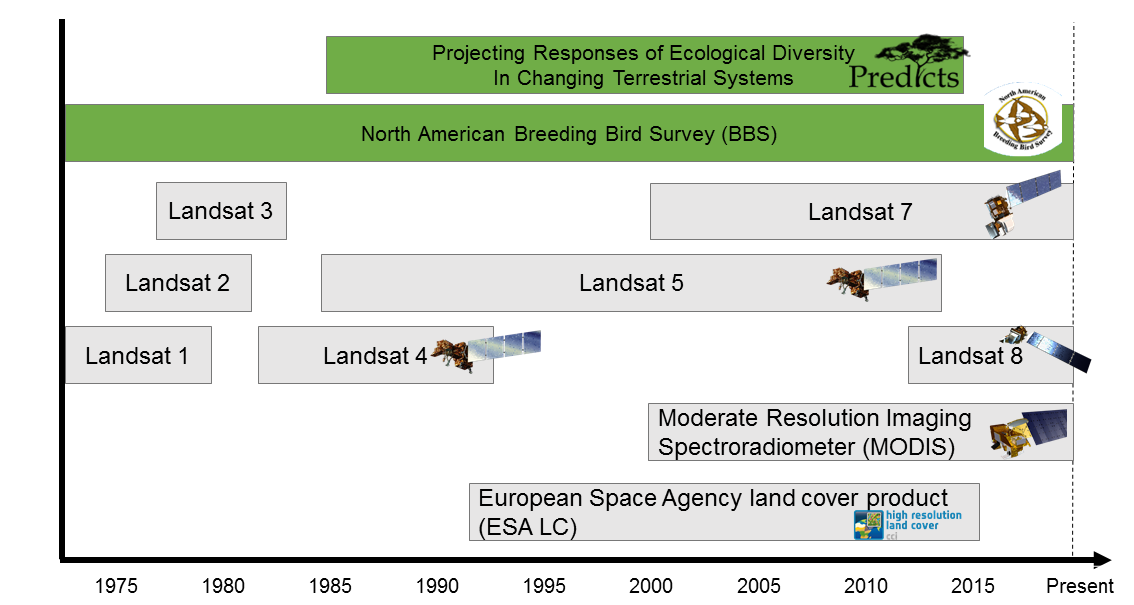
\includegraphics[width=1\textwidth]{chapter1/F01}
\caption{ Temporal coverage of biodiversity (green) and remote sensing (grey) datasets used in this thesis. Legacy Landsat missions (1-3) are shown for completeness only. }
\label{F01_01}
\end{figure}
% -------------------------------------------- %

Through technological advances humans have created a global spaceborne Earth observation system. The first satellite missions were used exclusively for military intelligence or weather observations. Since the mid-1970s satellite missions (Figure \ref{F01_01}), such as Landsat or later the Terra \& Aqua satellites with the Moderate Resolution Imaging Spectroradiometer (MODIS) sensor, were specifically designed to repeatedly photograph the Earth on a global scale \citep{Schaaf2002,Zhang2006,Kennedy2014}. These satellites carry highly sensitive sensors that measure the spectral reflectance from solar insolation. The near-infrared spectrum (Figure \ref{F01_02}\textbf{a}) has been recognized to be particularly useful for monitoring the photosynthetic activity of vegetation and can be quantified through “vegetation indices” \citep{Tucker1979,Tucker1981,Pettorelli2005,Jiang2008}. Differences in the dynamics of vegetation indices (Figure \ref{F01_02}\textbf{b}-\textbf{c}) can be used to identify land change globally. 

% ---------------- Figure 2 --------------------- %
\begin{figure}[htb]
\centering
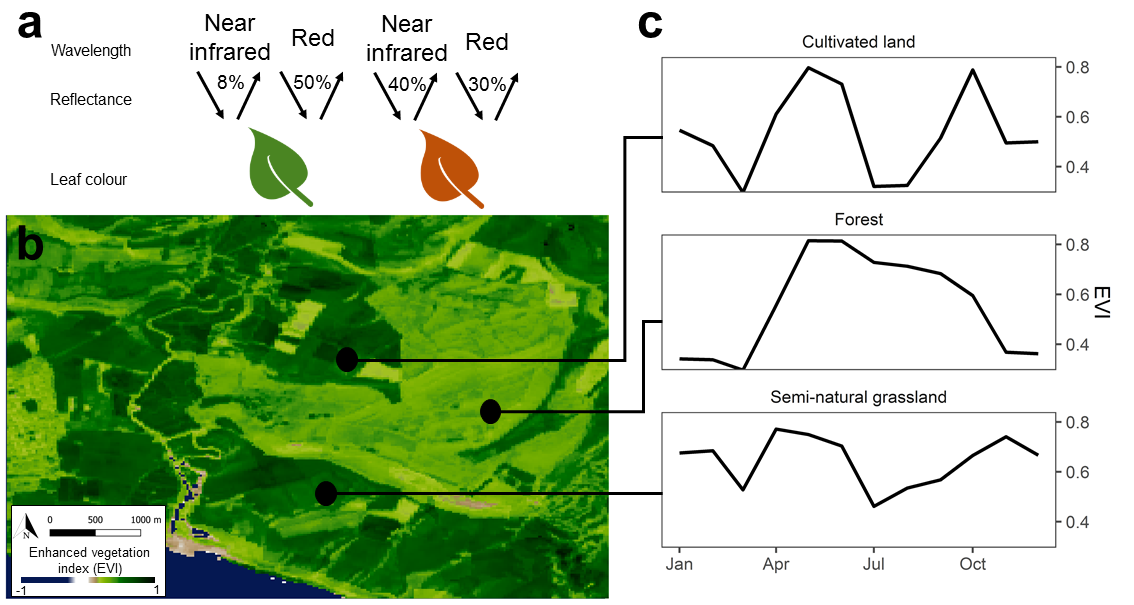
\includegraphics[width=1\textwidth]{chapter1/F02}
\caption{ (\textbf{a}) Schematic of how differences in spectral reflectances assist distinguishing leaf colour. (\textbf{b}) Map (Centre longitude: $0.165$\textdegree, latitude: $50.778$\textdegree) shows an annual maximum value composite (MVC) for 2018 of the Enhanced Vegetation Index (EVI) as calculated from the Landsat 8 mission. (\textbf{c}) Monthly MVC time series of three example sites (black points highlighted in \textbf{c}) of known land cover (cultivated land, forest, semi-natural grassland). }
\label{F01_02}
\end{figure}
% -------------------------------------------- %

Land change can be monitored using satellite-based remote sensing. A change on land can occur as either ‘conversion’ or ‘modification’, where the former is usually understood as “complete replacement of one land-cover type by another” \textendash\ \ie deforestation \textendash\ while the latter are “subtle changes” \textendash\ \ie agricultural intensification \textendash\ that affect the character of a land cover \citep{Lambin2003,Lambin2006}. Spatial estimates of the Earth’s land cover are commonly derived through a classification of remotely-sensed spectral reflectances \citep{DeFries1994,Hansen2000,DiGregorio2000}. However, these spatial estimates could often not be temporally compared because of classification biases and thematic inconsistencies \citep{VERBURG2011,Estes2018} and \textendash\ until recently \textendash\ little progress has been made to quantify land change globally. Novel algorithms and processing frameworks have been developed to quantify land change from temporal dynamics of spectral reflectances measuring photosynthetic activity \citep[Figure \ref{F01_02}\textbf{c}, ][]{Lhermitte2011,Gomez2016,Zhu2017}. With increasing availability and accessibility of satellite data \citep{Wulder2015} and computational power \citep{Gorelick2017} land changes have been quantified globally \citep{Hansen2013,Pekel2016,Li2018,Song2018}, creating new opportunities to  assess impacts of land change on biodiversity.   


\subsection{The impacts of past land change on local biodiversity}
\label{C01_0102}

% ---------------- Figure 3 --------------------- %
\begin{wrapfigure}{r}{0.5\textwidth}
  \begin{flushright}
    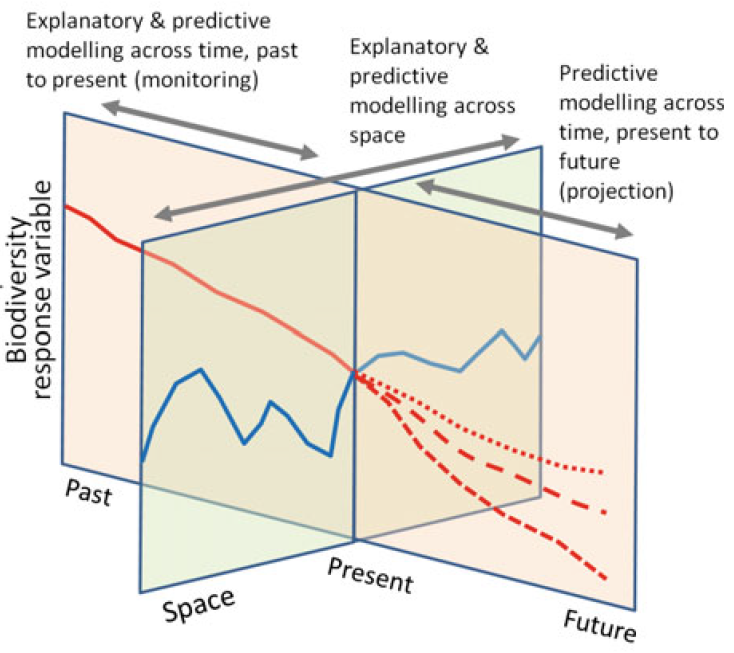
\includegraphics[width=.5\textwidth]{chapter1/F03}
  \end{flushright}
  \caption{ Schematic how a biodiversity response variable (red) can be estimated using environmental predictors (blue) in space and time. Adapted from \cite{Ferrier2017}. }
  \label{F01_03}
\end{wrapfigure}
% -------------------------------------------- %

Land changes can have immediate and/or delayed impacts on local biodiversity. They can act as disturbance affecting the stability of an ecosystem \citep{Pimm1984,Scheffer2003}, causing an immediate reduction in the number of species and individuals \citep{Nimmo2015,Ratajczak2018}. In addition, land changes can have delayed impacts on local biodiversity that persist for decades \citep{Martin2013,Moreno-Mateos2017} or centuries \citep{Vegas-Vilarrubia2011,McMichael2017}. Previous studies that investigated lasting influences of past land change \textendash\ varyingly described as “land-use history” or “landscape history” \citep{Bellemare2002,Foster2003,Ewers2013} or “management legacies” \citep{Perring2015} \textendash\ on biodiversity explained these influences through a number of mechanisms (Figure \ref{F01_04}, Table \ref{T01_01}).

% ---------------- Figure 4 --------------------- %
\begin{figure}[htb]
\centering
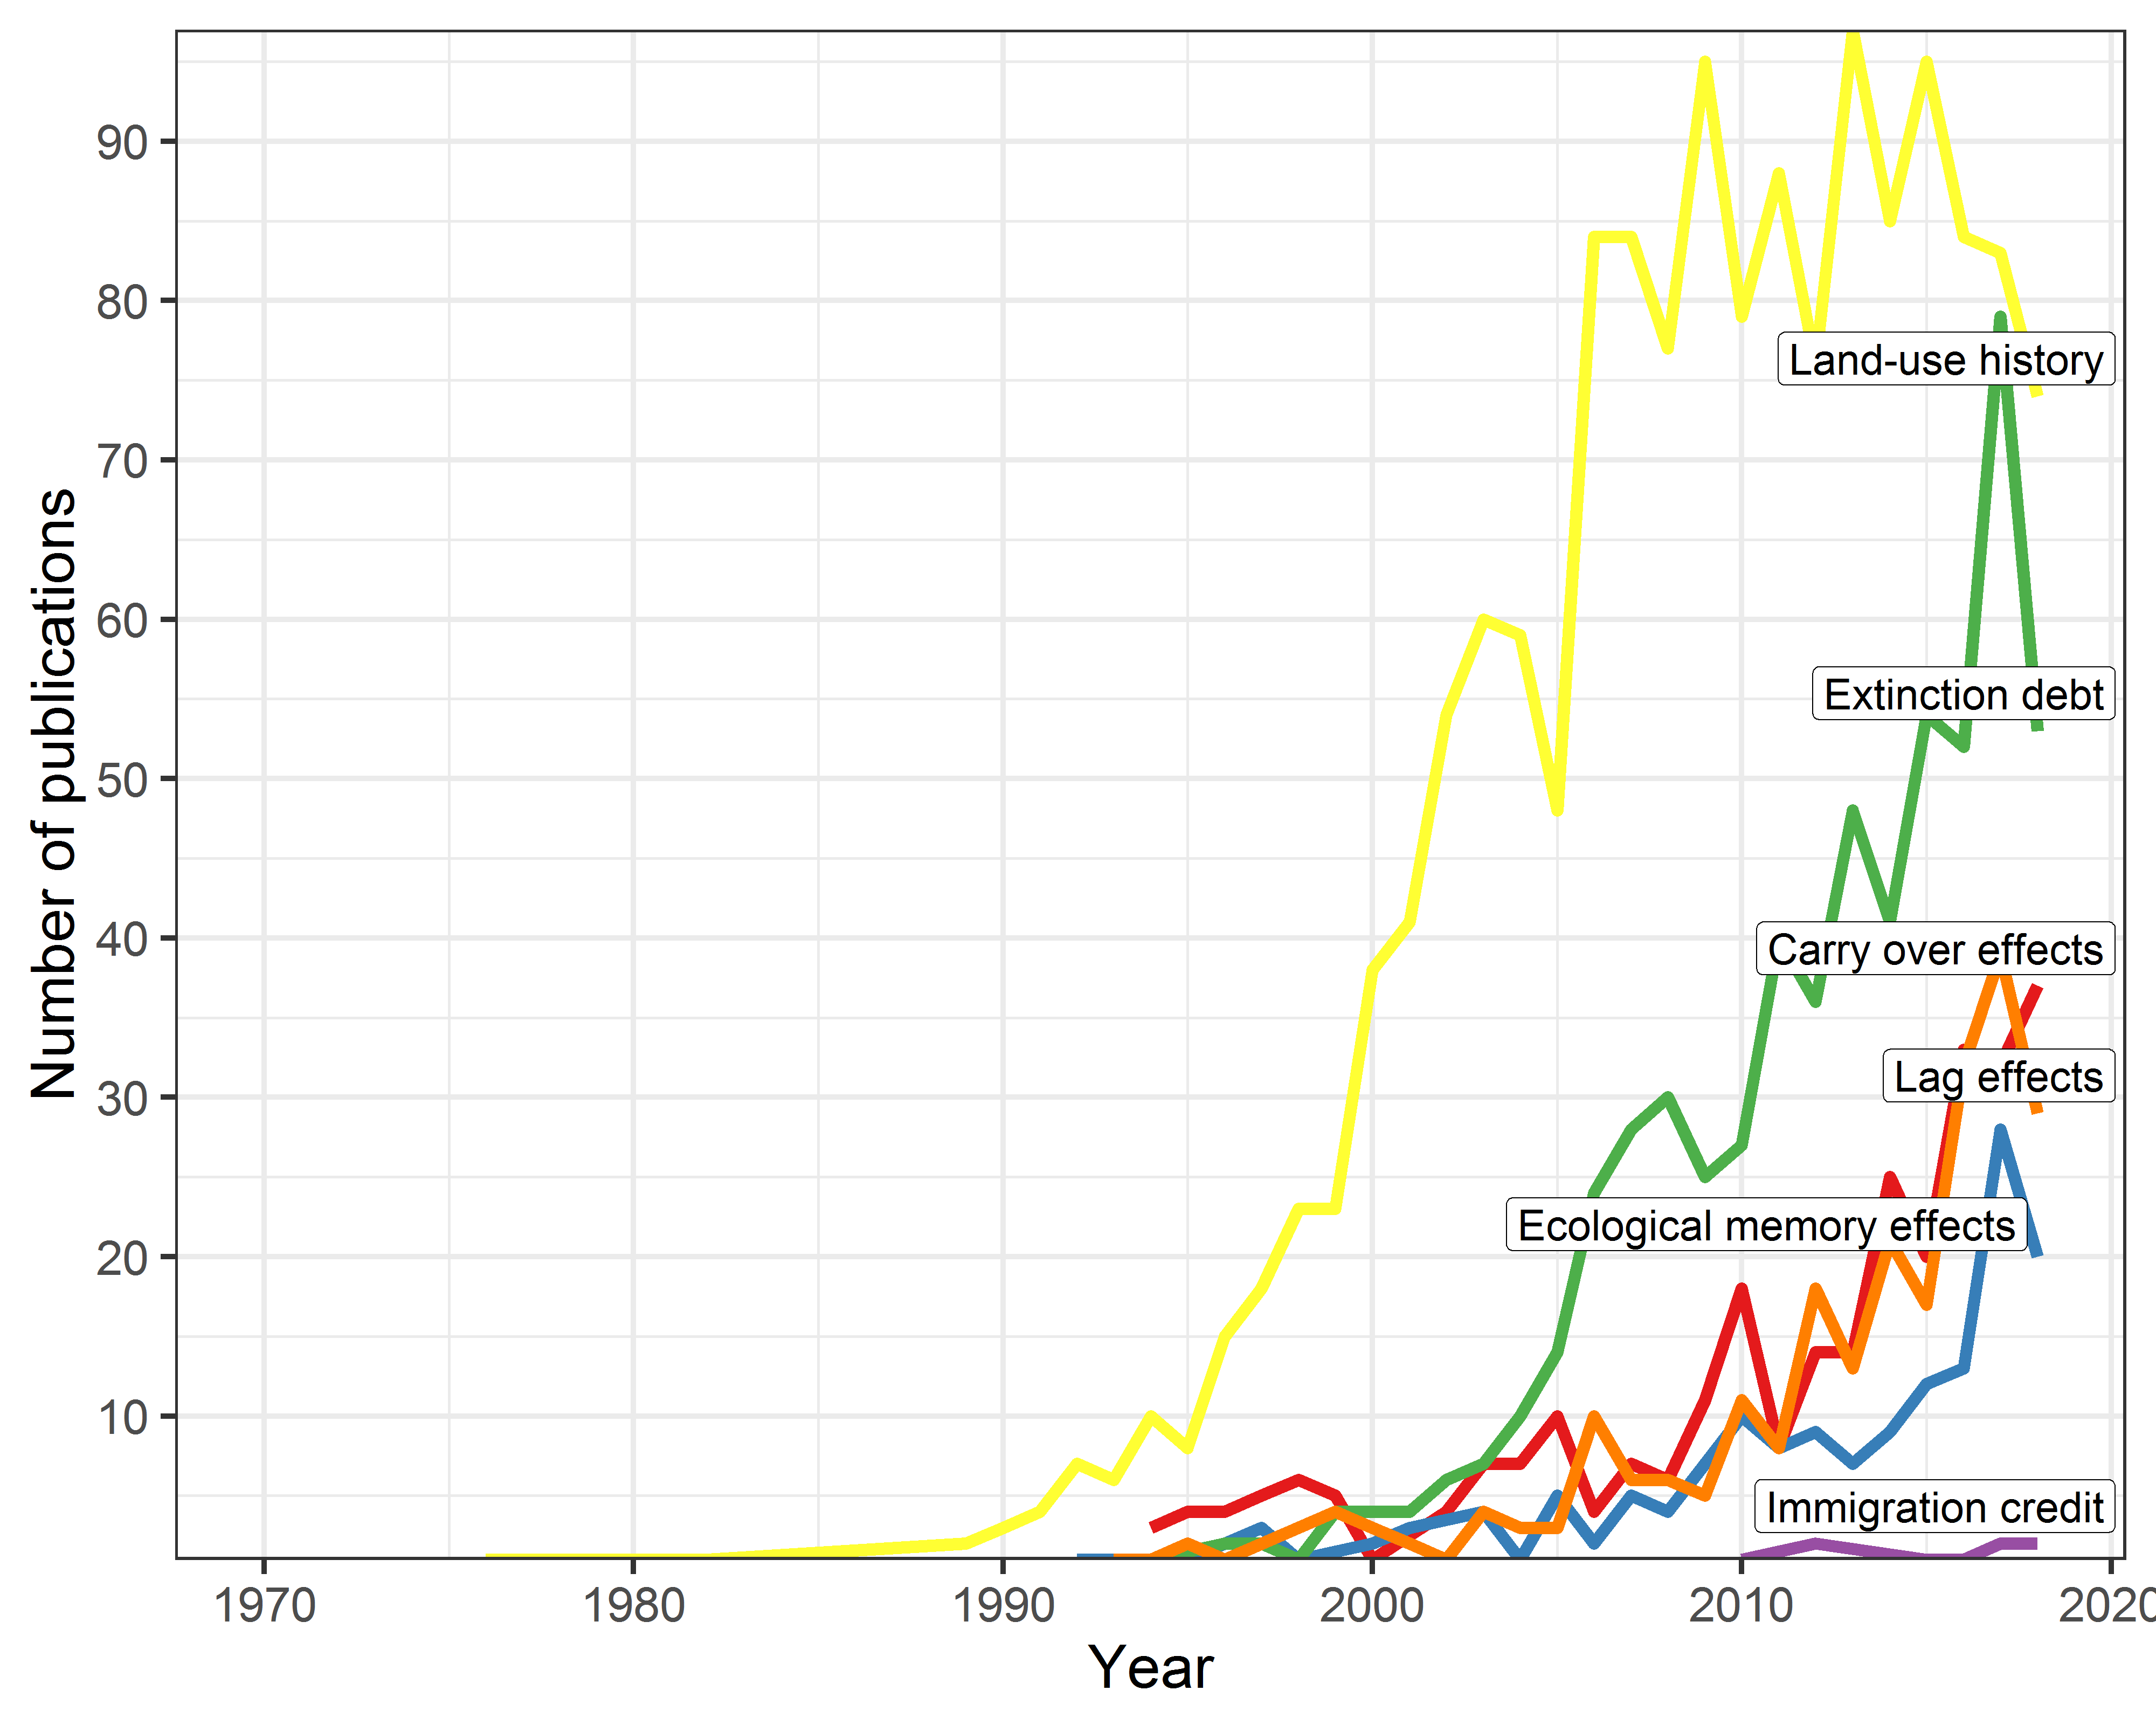
\includegraphics[width=1\textwidth]{chapter1/F04}
\caption{ Number of publications investigating terms and descriptions referring to biotic lag effects as queried from Web of Science\textsuperscript{TM} (WOS). A WOS search was conducted on the 5\textsuperscript{th} January 2019 limited to the Environmental sciences and ecological literature between 1900 and 2019 including as search topic “land-use histor*” (yellow), “extinction debt*” (green), “lag effect*” (orange), “carry*over effect*” (red), “ecological memory effect*” (blue) and “immigration credit*” (purple).  }
\label{F01_04}
\end{figure}
% -------------------------------------------- %

Several terms have been proposed to explain lasting impacts of past land change on local biodiversity (Table \ref{T01_01}). The term “extinction debt” describes the delayed extinction of species following a loss of habitat \citep{Balmford1996,Kuussaari2009,Wearn2012} and for many vertebrate species an extinction debt is usually “paid off” \textendash\ \eg the time until local population is fully extinct \textendash\ over a few years up to a century depending on the initial population size and species functional traits \citep{Halley2016}. Similarly, local biodiversity can also be influenced by an “immigration credit“, that is the delayed immigration of species from regional source populations after land change \citep{Jackson2010,Hylander2013}. Many species populations retain an “ecological memory” \citep{Peterson2002,Bengtsson2003,Ogle2015} of past land changes, reducing population growth and affecting species fitness and survival in subsequent years as “carry over” effect \citep{Harrison2011}. Collectively those terms can broadly be described as “biotic lag” effects (Table \ref{T01_01}), which are lasting or lagged effects of past changes in environmental factors that continue to influence present biodiversity. Knowledge about lasting impacts of land change can assist in planning management interventions \citep{Standish2014} and should be considered in broad-scale biodiversity models.  

Most existing regional and global assessments, models and scenarios of biodiversity \citep[\eg \ those included in the Intergovernmental Science-Policy Platform on Biodiversity and Ecosystem Services (IPBES) assessments, ][]{Alkemade2009,Pereira2010,Newbold2015} ignore lasting impacts of past land change. These assessments usually consider only concurrent differences in land-use/land-cover (Figure \ref{F01_03}) and may therefore partially misrepresent biodiversity change. Delayed impacts of past land change may accumulate together with other drivers \textendash\ such as climate change or species invasions \textendash\ of biodiversity change \citep{Essl2015,Essl2015a} potentially increasing the number of future species extinctions \citep{Dullinger2013}. To mediate the ongoing loss of biodiversity \citep{Mace2018}, robust estimates of the lasting impacts of land change on biodiversity need to be derived.

% ---------------- Table 1 ------------------- %
%\begin{landscape}
\begin{table}[ht]
\caption{Common terms and descriptions referring to lasting impacts of environmental changes on biodiversity}
\label{T01_01}

\newcolumntype{b}{X}
\newcolumntype{m}{>{\hsize=.6\hsize}X}
\newcolumntype{s}{>{\hsize=.4\hsize}X}

\begin{tabularx}{\textwidth}{ sbm }
\toprule
\textbf{Term} & \textbf{Description} & \textbf{Reference}   \\
\midrule

Land-use history  &  “Observed abiotic and biotic properties that are caused by past land use” & \citep{Foster2003,Perring2015} \\

Extinction debt & “The number of species committed to delayed extinction following a forcing event” &  \citep{Tilman1994,Kuussaari2009} \\

Immigration credit & “The number of species committed to delayed immigration following a forcing event” & \citep{Jackson2010} \\

Ecological memory & “The degree to which an ecological process is shaped by past modifications of the landscape, biotic and abiotic factors.” & \citep{Padisak1992,Peterson2002,Bengtsson2003,Ogle2015} \\

Carry-over effect & “Situation in which an individual’s previous history and experience explains their current performance in a given situation” & \citep{Harrison2011,OConnor2014} \\

Biotic lag &  Term summarizing the observed difference in biodiversity caused by lasting or lagged effects of past environmental changes  & \citep{DePalma2018} and this thesis   \\ \bottomrule

\end{tabularx}

\end{table}
% -------------------------------------------- %

\subsection{Linking satellite-based remotely-sensed land change with local biodiversity }
\label{C01_0103}

Remote sensing data can be useful for biodiversity models. Remotely-sensed land-surface conditions have been used to describe the biophysical state of species habitats \citep{Kerr2003}, identify critical life-history periods \citep{Pettorelli2005}, map species distributions \citep{He2015a} or as a proxy for predicting biodiversity patterns \citep{Rowhani2008,Rocchini2015,Hobi2017}. However, uncertainties remain in the usability of remote sensing data for different measures of biodiversity \citep{Oldeland2010}, for taxonomic groups \textendash\ where biodiversity measures are sometimes poorly correlated with photosynthetic activity \citep{Adler2011} or spectral dissimilarity \citep{Schmidtlein2017} \textendash\ or for many, previously unassessed geographic regions. Especially the temporal domain (Figure \ref{F01_02}\textbf{b}-\textbf{c}), including land change \textit{per se}, is often ignored \citep{Kennedy2014}. New frameworks are needed to establish links between remotely-sensed land change and local biodiversity.

Land change can be characterized by key attributes that may have varying impacts on local biodiversity (Figure \ref{F01_05}\textbf{a}). \cite{Watson2014} provided a conceptual framework that distinguishes between four attributes of land change: (\textbf{1}) The magnitude of land-change events, (\textbf{2}) the frequency of land-change events over time, (\textbf{3}) the time span since a land change occurred, and (\textbf{4}) the temporal sequence of land use and/or land cover categories (Figure \ref{F01_05}\textbf{a}). Ecological theory, experiments and simulations demonstrated that local biodiversity can be affected by these attributes (Figure \ref{F01_05}\textbf{b}). Land changes of larger magnitude are expected to affect biodiversity more \citep{Scheffer2001,Dornelas2010,Svensson2012,Ratajczak2018} and \textendash\ by removing poor dispersing \citep{Tilman1997} and specialist species \citep{Christensen2018} \textendash\ potentially reducing the stability of species assemblages \citep{Scheffer2001,Oliver2015,Hautier2015}. In many regions of the world, land changes vary in frequency \citep{Kleyer2007} impacting local biodiversity \citep{Valtonen2013,Lawson2015}, especially if those impacts accumulate in a short period of time \citep{Essl2015,Ratajczak2018}. Biodiversity measures can often recover to reference levels (\ie a temporal or spatial baseline) following land change, depending on the time passed \citep{Chazdon2003,Laurance2011,Martin2013}. Lastly, and commonly investigated, is the temporal sequence of land use and/or land cover types \citep{Harding1998,Chazdon2003,Foster2003}, where local biodiversity tends to be more altered at sites with past anthropogenic use. However, the impact of these four attributes of land change on local biodiversity has rarely been comparatively assessed globally and across taxonomic groups.

% ---------------- Figure 5 --------------------- %
\begin{figure}[htb]
\centering
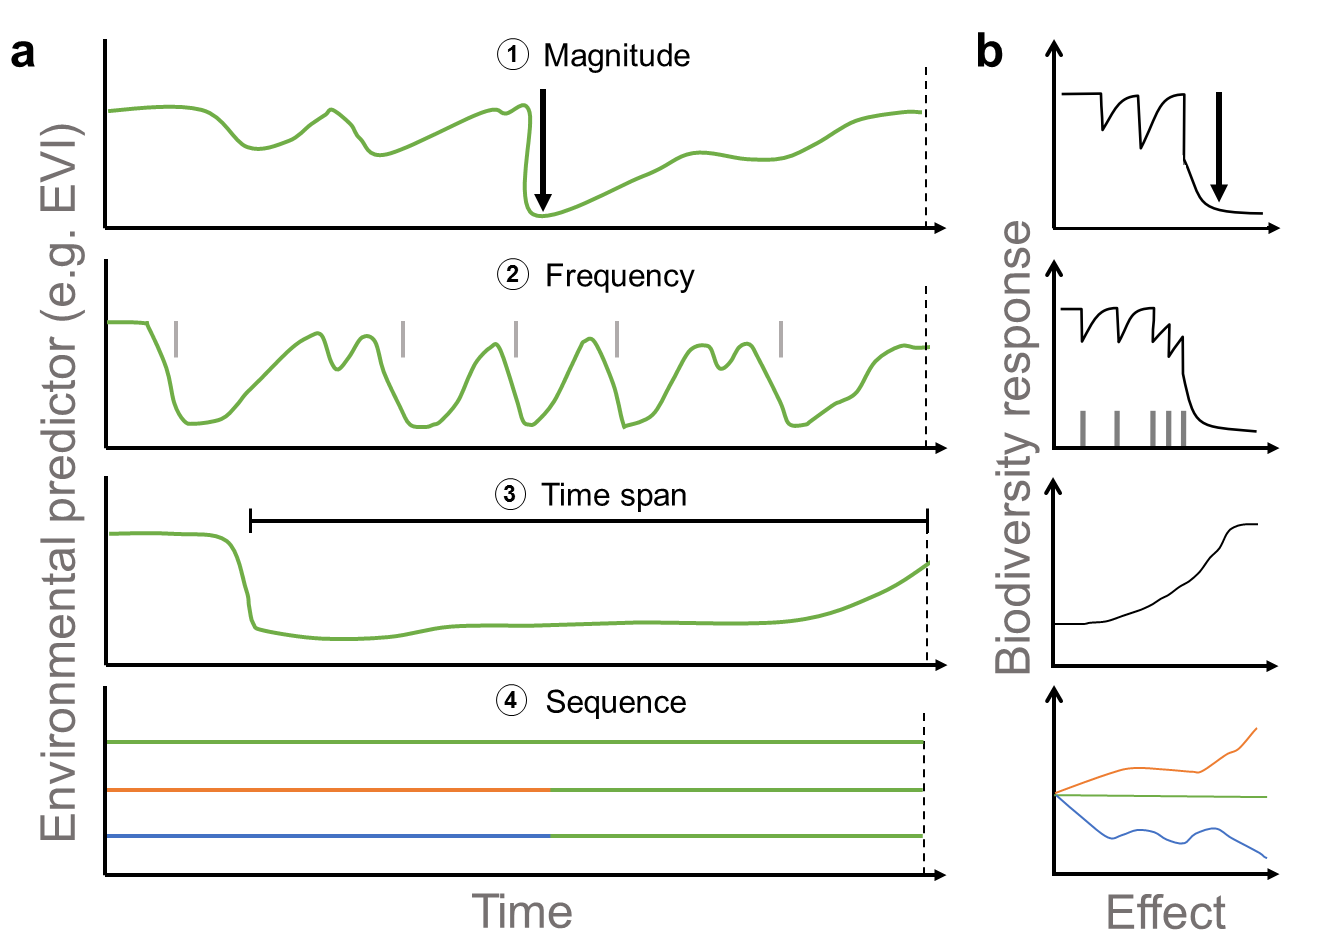
\includegraphics[width=1\textwidth]{chapter1/F05}
\caption{ (\textbf{a}) Conceptual framework \textendash\ inspired by \cite{Watson2014} \textendash\ how sites can differ by attributes of land change, namely (1) magnitude, (2) frequency, (3) time span and (4) sequence. Dashed lines indicate the start of biodiversity sampling with the y-axis representing an environmental predictor such as the Enhanced Vegetation Index (EVI). (\textbf{b}) Assumed response of biodiversity to varying land change attributes with x-axis indicating the strength of effect in units of each individual attribute.  }
\label{F01_05}
\end{figure}
% -------------------------------------------- %

\subsection{Thesis aims and structure}
\label{C01_0104}

The overall aim of my thesis is to investigate how local biodiversity is impacted by land changes globally and whether those impacts vary with attributes of land change  (Figure \ref{F01_05}). I do so by linking satellite-based remotely-sensed estimates of land change with measures of local biodiversity globally   (Figure \ref{F01_06}). The four main analytical chapters (Chapter \ref{C02}-\ref{C05}) of this thesis each address multiple of the four outlined attributes of land change (Figure \ref{F01_06}). They each serve as independent articles that have either been published, submitted or are in principle suitable for submission to an academic journal.

% ---------------- Figure 6 --------------------- %
\begin{figure}[htb]
\centering
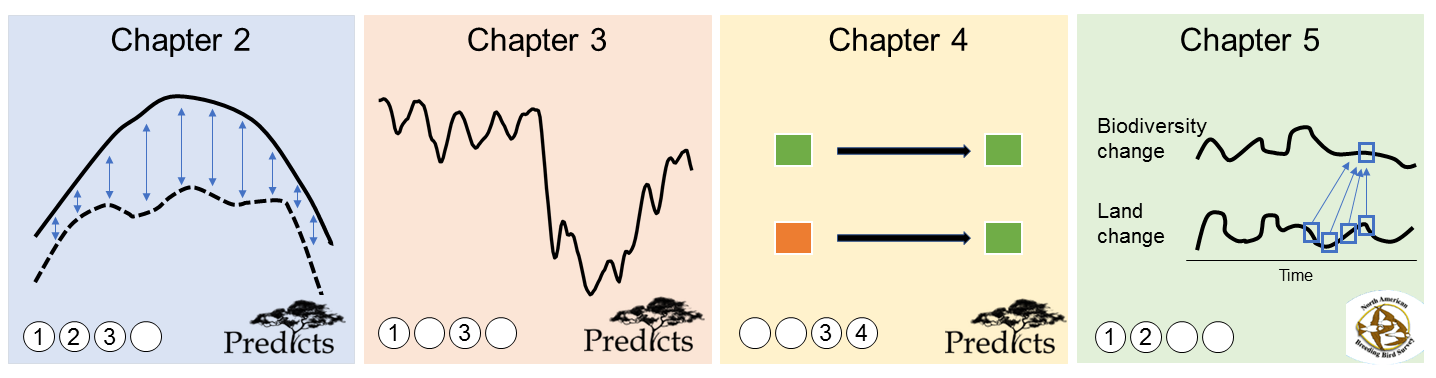
\includegraphics[width=1\textwidth]{chapter1/F06}
\caption{ Schematic outline of the four approaches (Chapter \ref{C02}-\ref{C05}) linking local biodiversity with remotely-sensed land change data, with lines and icons representing differences in intra-annual land dynamics (Chapter \ref{C02}), an abrupt land change of large magnitude (Chapter \ref{C03}), different land-cover sequences (Chapter \ref{C04}) and correlating temporal change in land and biodiversity observed at the same sites (Chapter \ref{C05}). Numbers in circles at the bottom left (1-4) indicate which attributes of land change from \cite{Watson2014} are considered in each approach (see Figure \ref{F01_05}\textbf{a}), while logos indicate the biodiversity data used (PREDICTS or United States BBS data). }
\label{F01_06}
\end{figure}
% -------------------------------------------- %

Chapter two assesses whether considering past land-surface conditions in the six years before biodiversity sampling can assist in explaining differences in local biodiversity. I developed an analytical framework that captures all differences between time series of remotely-sensed land-surface conditions \textendash\ such as land changes with varying magnitude or inter-annual frequency \textendash\ in a single metric, which was then linked with differences in species assemblage composition across taxonomic and functional groups globally. 

The third chapter focusses on how abrupt land changes \textendash\ characterized by shifts in magnitude or trend and varying time passed \textendash\ continue to influence local biodiversity. I assembled time series of Landsat imagery globally (Figure \ref{F01_01}\textbf{a}) and subjected them to a change-detection algorithm to detect abrupt land changes. A hierarchical analysis was conducted to assess if and how strongly local biodiversity differs between sites with and without a land change in the past. The assumption is that local biodiversity is more affected by abrupt land changes of greater magnitude that occurred more recently.

In chapter four I investigated how local biodiversity differs between sites with varying land-cover sequences of land cover change as derived from a global, temporally consistent land-cover product for the years 1992 to 2015. The assumption is that local biodiversity is higher at sites with a past land-cover change compared to those without, if the preceding land cover was less anthropogenically modified. In addition, this chapter investigates how past land-cover sequences can influence global and national biodiversity projections and argues for including estimates of past land change in biodiversity projections.

In contrast to previous chapters, in the fifth chapter I investigate if local biodiversity change can be linked to landscape-wide land changes. Estimates of bird diversity change from repeated breeding bird surveys (BBS data, Figure \ref{F01_01}) were correlated with estimates of preceding and concurrent land change at the landscape scale quantified from time series of Landsat imagery. I furthermore investigate whether the explanatory power of landscape-wide land changes on bird diversity change varies in space, time and across functional groups of bird species. The assumption is that bird diversity declines more in landscapes with a greater proportion of land changes.

The thesis concludes with the sixth chapter, which provides a synthesis of the presented work, discusses all findings in relation to previous studies, and mentions shortcomings and promising directions for future research.

\clearpage
%\bibliography{content/01Chapter}

%\appendix
%\begingroup
%  Blank

%\endgroup
 %Introduction
  \chapter{ Local species assemblages are influenced more by past than current dissimilarities in photosynthetic activity}
\label{C02}
%\addcontentsline{toc}{chapter}{Chapter 2}
%\markboth{}{Local species assemblages are influenced more by past than current dissimilarities in photosynthetic activity}

Most land on Earth has been changed by humans and past changes of land can have lasting influences on current species assemblages. Yet few globally representative studies explicitly consider such influences even though auxiliary data, such as from remote sensing, are readily available. Time series of satellite-derived data have been commonly used to quantify differences in land-surface conditions such as vegetation cover, which will among other things be influenced by anthropogenic land conversions and modifications. Here we quantify differences in current and past (up to five years before sampling) vegetation cover, and assess whether such differences differentially influence taxonomic and functional groups of species assemblages between spatial pairs of sites. Specifically, we correlated between-site dissimilarity in photosynthetic activity of vegetation (the Enhanced Vegetation Index) with the corresponding dissimilarity in local species assemblage composition from a global database using a common metric for both, the Bray-Curtis index. We found that dissimilarity in species assemblage composition was on average more influenced by dissimilarity in past than current photosynthetic activity, and that the influence of past dissimilarity increased when longer time periods were considered. Responses to past dissimilarity in photosynthetic activity also differed among taxonomic groups (plants, invertebrates, amphibians, reptiles, birds and mammals), with reptiles being among the most influenced by more dissimilar past photosynthetic activity. Furthermore, we found that assemblages dominated by smaller and more vegetation-dependent species tended to be more influenced by dissimilarity in past photosynthetic activity than prey-dependent species. Overall, our results have implications for studies that investigate species responses to current environmental changes and highlight the importance of past changes continuing to influence local species assemblage composition. We demonstrate how local species assemblages and satellite-derived data can be linked and provide suggestions for future studies on how to assess the influence of past environmental changes on biodiversity.

\section{Introduction}
\label{C02_01}
Throughout the Earth's history, land has changed constantly by a combination of natural and anthropogenic forces. Palaeontological evidence indicates that humans have transformed approximately 75\% of the land at least once \citep{Ellis2010,Ellis2011}, with changes in many land-surface conditions, such as vegetation cover, accelerating since the beginning of the industrial revolution \citep{Lambin2006,Steffen2015}. Changes in vegetation cover may be caused by climatic factors, such as CO\textunderscript{2} fertilization or altered precipitation patterns \citep{Zhu2016}, or anthropogenically caused land conversions, such as deforestation, re- and afforestation \citep{Dupont2003,Hansen2013,Muller2014} or land modifications, such as degradation, intensification \citep{Gibbs2015,Rufin2015} or return to less intensive forms of land use \citep{Zomer2016}. Over time, these changes have shaped both land and species assemblages in complex ways \citep{Foster2003,Watson2014,Perring2015}.

Most global meta-analyses investigating the influence of differences in vegetation cover on species assemblages have assumed that any difference in vegetation cover at the time of biodiversity sampling is the dominant influence
\citep{Stein2014, Newbold2014b, Newbold2015, Alroy2017}. However, this assumption might be incorrect as assemblages can be heavily influenced by legacy effects of past changes in vegetation cover \citep{Foster2003, Watson2014, Ogle2015, Perring2015}. For the recent past (\eg, up to five years prior to biodiversity sampling), ecological memory or carry-over effects, \ie the capacity of past events to influence present and future ecological assemblages \citep{Harrison2011, OConnor2014, Ogle2015}, have been proposed as mechanisms that shape species assemblages. These effects can arise through site-specific environmental factors, for instance altered conditions because of agricultural practices \citep{Perring2015,Perring2018} or different sequences and successional recovery from changes in past vegetation cover \citep{Johnson2008,Walker2010,Watson2014}. No detailed global analysis to date has explicitly considered the influence of both current and past differences in vegetation cover on current species assemblages.

While some differences in species assemblages can be traced back to changes in vegetation cover in the late quaternary \citep{Vegas-Vilarrubia2011,McMichael2017}, there is some evidence that changes in vegetation cover in the more recent past can influence plant \citep{Jakovac2016}, invertebrate \citep{Valtonen2013} or vertebrate assemblages \citep{Newton2014, Cole2015, Graham2015}. However, this has — to our knowledge — not been assessed comparatively across multiple taxonomic groups. Furthermore, it is likely that species with specific traits, such as certain body size and/or trophic level, may be differentially affected by past changes in vegetation cover because of differences in their metabolic rate (for animals), longevity or dispersal abilities \citep{Sutherland2000, Brown2004, Speakman2005,Thomson2011,DePalma2015}. Depending on the type and magnitude of a past changes in vegetation cover (as a proxy for land-surface changes) plant assemblages can either be dominated by small, fast sprouting or taller, nutrient-demanding species \citep{Jakovac2016,Perring2018}. Until now, our understanding of the influence of past differences in vegetation cover on species assemblages has been limited to case studies focused on specific regions or certain taxonomic and functional groups. However, a recently published globally representative dataset on species assemblages of broad taxonomic coverage \citep{Hudson2016} and globally available satellite-derived data enable us to consider explicitly both current and past differences in land-surface conditions.

Satellite-derived data can provide internally consistent estimates of how land differs across time and space \citep{Pettorelli2005, Kennedy2014}. Land-surface conditions such as photosynthetic activity of vegetation can be quantified using spectral indicators from satellite-derived data \citep{Gamon1995, Zhang2006}. Changes in photosynthetic activity of vegetation can be related to both climatic \citep{Fensholt2012, Zhu2016} and anthropogenic factors such as land conversions and modifications \citep{Lambin2003, Muller2014}. Subtle differences in vegetation dynamics (as measured by various satellite-derived vegetation indices), such as faster greening rate or differing seasonal amplitude, between years have been used to characterize land change \citep{Lambin1994, Linderman2005, Lupo2007}. Recent studies have used such differences to identify changes in land use such as pasture use intensity \citep{Rufin2015}, fallow periods in croplands \citep{Estel2015, Tong2017}, small-scale deforestation \citep{DeVries2015b} and broad scale land degradation and intensification \citep{deJong2011,Muller2014}. Dissimilarity metrics describing the entirety of recent land history (\eg including both differences in land use and land cover as well as climatic and site-specific factors) can be calculated between spatial pairs of time series as the overall dissimilarity in photosynthetic activity \citep{Linderman2005, Lhermitte2011}. Increasingly such methods have been linked to dissimilarity in local species assemblage composition \citep{Rowhani2008, Goetz2014, Nieto2015, Hobi2017}, however few studies have explicitly distinguished between current and past dissimilarity in photosynthetic activity.
	
Here we use a time series dissimilarity metric (the Bray-Curtis index) to quantify dissimilarity in a land-surface attribute, e.g. photosynthetic activity of vegetation, among spatial pairs of sites in the Projecting Responses of Ecological Diversity In Changing Terrestrial Systems (PREDICTS) dataset \citep{Hudson2016}. We explicitly distinguish between dissimilarity in current and past photosynthetic activity (BC\textunderscript{EVI}), defined here as the five years prior to the ‘current’ year, and assess how they influence compositional dissimilarity (BC\textunderscript{Biodiversity}) between species assemblages among paired sites. This pairwise comparison approach allows us to investigate (\textit{i}) the overall influence of past relative to current dissimilarity in photosynthetic activity on species assemblages where we hypothesize that the influence of past dissimilarity increases with longer past periods considered. Furthermore, we investigate (\textit{ii}) whether different taxonomic groups respond differently to past dissimilarity in photosynthetic activity, and (\textit{iii}) if species with particular functional characteristics, \ie, those that are smaller and/or more vegetation-dependent, are more affected by past dissimilarity in photosynthetic activity than others. 


\section{Data and Methods}
\label{C02_02}
\subsection{Remotely-sensed data}
\label{C02_0201}
A temporal profile of spectral reflectance values was derived from the Moderate Resolution Imaging Spectroradiometer (MODIS) sensor on board NASA’s Terra and Aqua satellites. Since the year 2000, MODIS has provided continuous spectral data of medium-scale resolution (nominal \textasciitilde500 m resolution) with high temporal revisit rates (a global image collection is taken every day) \citep{Schaaf2002}. We used the Bidirectional Reflectance Distribution Function and Albedo (BRDF) product (MCD43A4.005), which aggregates the highest quality daily spectral reflectance values into 8-day composites of seven spectral bands \citep{Schaaf2002}. Google Earth EngineTM was used to download and process temporal profiles of all spectral bands for each site \citep{Gorelick2017}. We calculated a spectral index measuring photosynthetic activity (the two-band Enhanced Vegetation Index – EVI; \cite{Jiang2008}), which is based on a ratio between the near-infrared (nir, 841-876 nm) and red (red, 620-670 nm) spectral band \( EVI = 2.5 * \frac{(nir - red)}{(nir + 2.4 * red + 1)} \). We used the EVI as it has been designed to reduce atmospheric contamination and not to saturate in high biomass regions such as tropical rainforests \citep{Huete2002,Jiang2008}. We applied the following pre-processing steps (also see flowchart in Appendix Figure \ref{SI02_01}) to the nir and red BRDF bands individually to fill missing observations and filter out extreme data points. 

First, we detected and removed extreme outliers in the BRDF data that may have been introduced by cloud shadows, atmospheric haze, inversion errors or sensor failures. We calculated the absolute difference of all values from the median relative to the total median absolute deviation (MAD) of all values \citep{Leys2013}. Pixels which were more than a conservative threshold of two units deviation \citep[but see][]{Leys2013} away from the MAD as well as greater than 99\% of all other difference values were set to missing. This data-defined threshold removed only the most extreme outliers and retained fluctuations that are within the bounds of median conditions. We chose this procedure rather than using the MODIS BRDF quality data set (stored in the separate MCD43A2.005 product) to maintain the maximum number of observations assuming that bad quality inversions of the BRDF product are filtered and smoothed out by subsequent pre-processing steps.

Second, we interpolated missing values using a Kalman filter, a smoother for estimating missing data points based on preceding data \citep{Kalman1960}. Previous studies have shown that Kalman filters perform well in filling gaps in BRDF time-series especially in data-poor regions \citep{Samain2008}. The best model for the Kalman filter for a given time-series was estimated using the “forecast” R package (“auto-arima” function) by selecting the model with the lowest Akaike Information Criterion (AIC) \citep{Hyndman2008}. We only interpolated consecutive gaps $\leq 40$ days (\ie five consecutive 8-day BRDF composites) as longer interpolations would reduce our ability to detect short-term changes in photosynthetic activity.  We excluded all time-series from further analyses with more than 50\% remaining missing data (average proportion of missing data = 6.32 $\pm$ 10.31\%) in the time period considered (see Appendix Figure \ref{SI02_02}). 

Lastly, we applied a Savitzky-Golay filter (filter length = 5, “signal” R-package) to reduce the amount of random noise remaining in the time series, but retain small abrupt changes that might occur \citep{Joensson2004}. The Savitzky-Golay filter performs well relative to other smoothing techniques in removing noise \citep{Kandasamy2013}. Our pre-processing steps aimed to remove influential outliers and random noise from each time series, but we cannot rule out that some non-informative noise has remained in the time series. From these pre-processed BRDF data we calculated the EVI for each 8-day composite \citep{Jiang2008}.

\subsection{Species assemblage data}
\label{C02_0202}
We used data on species’ abundance within local-scale assemblages from the PREDICTS database \citep[downloaded on 3 February 2016, see \ref{SI02_01}]{Hudson2016}, which is the largest global database investigating anthropogenic impacts on terrestrial species assemblages to date. The PREDICTS database has collated local-scale species assemblage records from the published literature (henceforth “sources”) comparing observations among at least two localities (henceforth “sites”) with differing land use or related pressures. Sources in the PREDICTS database having multiple sampling methodologies and taxonomic groups were split accordingly into different “studies”. Wherever sampling effort differed among sites within a study, we followed the approach of \cite{Newbold2014b} and adjusted abundance values assuming that recorded abundance increase linearly with effort. Each study was assigned to one of six higher taxonomic groups based on the sampled species identity (Plants, Invertebrates, Amphibians, Reptiles, Birds and Mammals). We grouped plants and invertebrates into single individual groups as there were insufficient data to divide them into smaller groups (\eg, functional divisions such as flying vs ground-living insects). Studies of fungi were dropped from the analyses because of insufficient data.

Of the 25224 sites with abundance data, we removed 6109 sites because their sampling durations spanned more than a year or because the start of biodiversity sampling differed by more than three months among sites within a study. This was done to avoid seasonal effects confounding any link between species assemblage composition and remote-sensing derived estimates. Furthermore, we removed 10248 sites from studies that sampled biodiversity before the 18th of February 2006 to ensure MODIS data availability for at least five years prior to biodiversity sampling. We chose to use a five-year period to allow sufficient MODIS coverage (since year 2000) for the majority of studies in the PREDICTS database (median biodiversity sampling start date = 2007-07-17). In total 8867 sites were suitable to be linked with MODIS remote-sensing data.

The spatial extent of biodiversity sampling at PREDICTS sites typically differs from the resolution of MODIS data. We used the Maximum Linear Extent (MLE) information within the PREDICTS database, which summarises the spatial extent of sampling within a study in metres \citep{Hudson2016}. Sites from a few studies had large MLE (up to 40 km) and after visual exploration, we decided to keep only those sites that were within the 99\% quantile of all MLE values (MLE < Q99 = 3000 m, removing 249 sites). Some studies had missing MLE information (25\% of all studies with abundance data, 728 sites), where no MLE estimate could be obtained during the PREDICTS data curation \citep{Hudson2016}. We filled missing MLE information with the average MLE estimate of each taxonomic group with corresponding sampling method, and any remaining missing MLE, for which no other combination of taxonomic group and sampling method had MLE estimates, with the average MLE for each taxonomic group. We tested the robustness of this assumption by removing 25\% of the existing MLE estimates at random and found interpolated MLE values to be reasonably accurate (r = 0.73, p < 0.001). We used the centre coordinates for the rest of the sites (mean MLE $\pm$ SD = 256.52 m $\pm$ 437.93 m) as their spatial extent roughly matched the nominal spatial resolution of the MODIS data (\textasciitilde 500 m). 

We excluded studies from our analyses where all study sites fell within a single MODIS grid cell, to suit our hierarchical statistical approach (see below). Some sites within a study could fall into the same MODIS grid cell, therefore for all further analyses we randomly selected one site per study per grid cell 100 times (See section on analysis – pairwise differences below for description of permutation procedure and Appendix Figure \ref{SI02_03} for a schematic), resulting in 100 different subsets that we used for all further analyses. Our final dataset included data from 198 studies with 4053 sites per permutation and model covering all major continents and most taxonomic groups (Figure \ref{F02_01}).

% ---------------- Figure 1 --------------------- %
\begin{figure}[ht]
\centering
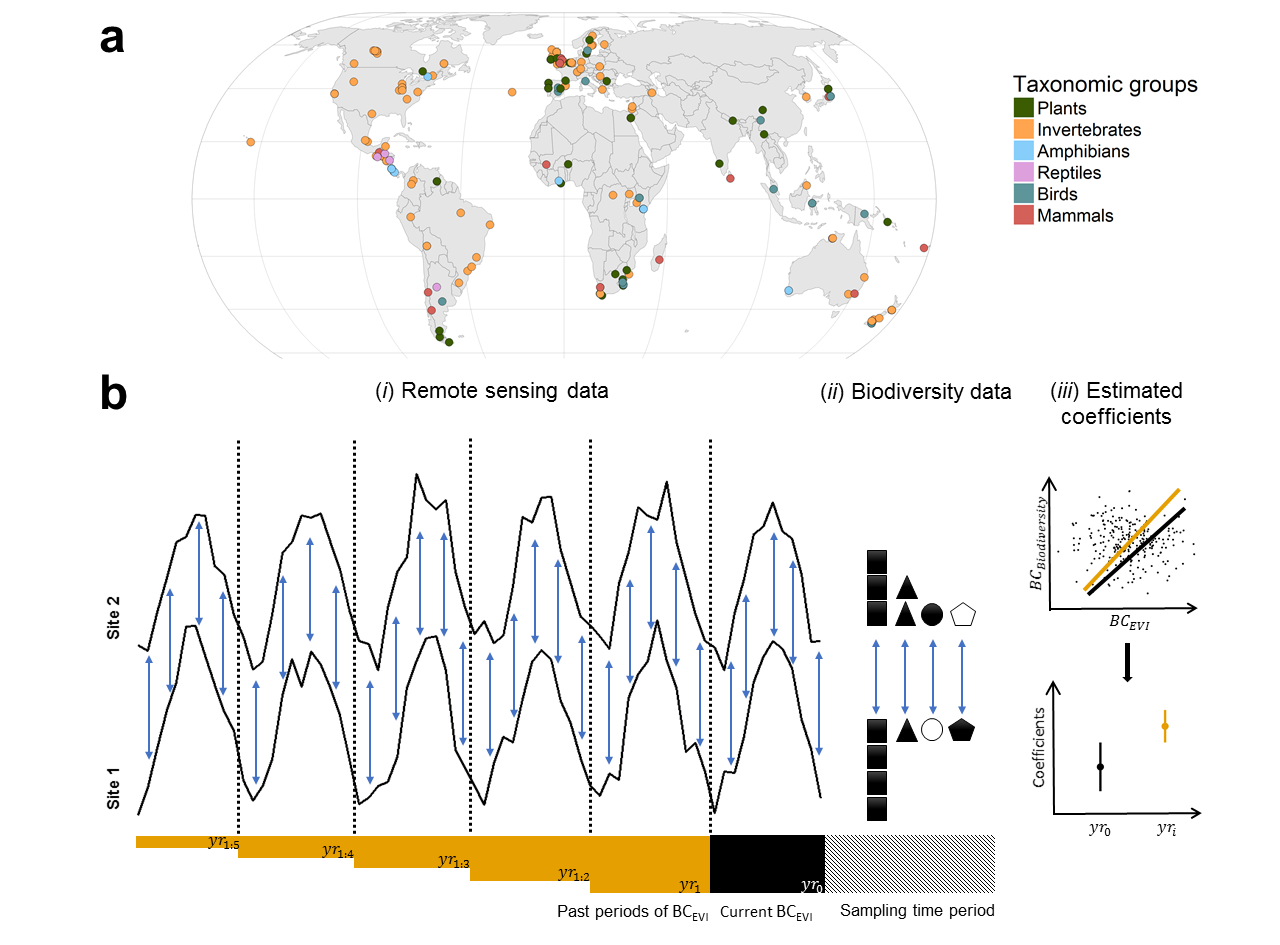
\includegraphics[width=1\textwidth]{chapter2/F01}
\caption{ (\textbf{a}) Locations of 198 species assemblage studies (centroid of each study) coloured by taxonomic group. (\textbf{b}) Diagram of the modelling approach to investigate influences of current and past dissimilarity in photosynthetic activity on species assemblages. The Bray-Curtis index (BC\textunderscript{EVI}) was calculated between pairs (blue arrows) of remote-sensing time series (black solid lines) and of species assemblages (BC\textunderscript{Biodiversity}) collected at paired sites. Independent statistical models were constructed for both current (i - black) and past BC\textunderscript{EVI} of varying length (ii - orange) and their model effects compared (iii – Estimated fixed effects).}
\label{F02_01}
\end{figure}
% -------------------------------------------- %

\subsection{Species trait compilation}
\label{C02_0203}
A species’ size and trophic level are two of the most basic traits for understanding differences in species assemblage structure \citep{Speakman2005,Terborgh2015}. We classified studies into size and trophic bins based on a simple majority: small (>0-9 g animal body mass or > 0-9 cm plant height), medium (10 – 99 g or 10-99 cm) or large species (>= 100 g or >= 100 cm), or predominantly herbivore, omnivore, carnivore or detritivore species, by estimating the dominant number of species (simple sum of measurement) within a study. Studies with species of predominantly unknown size or trophic level were removed from the analysis. We thus classified entire studies to the dominant bins as each study’s methodology would likely constrain the average size of animals or plants that can be observed. Data on average adult body mass (in g) were collected for mammals \citep{Jones2009} and birds \citep{Myhrvold2015}, while for plants we used height (in cm) data from the TRY database \citep{Kattge2011}. The estimates of species trophic levels originate from \cite{Kissling2014}, \cite{Wilman2014} and other sources of the literature for invertebrates (obtained from Laura Bentley, Imperial College London, UK). For species for which size or trophic level data were unavailable, we used the genus-wide average for size and the most common trophic level (at least 95\% of all species with data within a genus). We excluded studies (N=8) from further analyses where no clear majority of species (> 50\%) could be assigned to one of the bins (Appendix Figure \ref{SI02_04}), leaving a total of 65 studies with size information and 130 studies with trophic information. 

\subsection{Analysis - Pairwise dissimilarity}
\label{C02_0204}
We linked dissimilarity in photosynthetic activity of vegetation with compositional dissimilarity in species assemblages globally. Specifically, we examined the differential influence of “current” (yr\textunderscript{0}, as the 365 days prior to species assemblage sampling) and “past” (yr\textunderscript{i}, the i years prior to the current year, where $i = 1,..,5$) dissimilarity in photosynthetic activity between spatial pairs of sites (Figure \ref{F02_01}\textbf{b}, Appendix Figure \ref{SI02_03}). We separately considered past periods of increasing lengths (in years, so yr\textunderscript{1}, yr\textunderscript{1:2}, yr\textunderscript{1:3}, yr\textunderscript{1:4}, yr\textunderscript{1:5}). For example, if species assemblage sampling was conducted from the 1st of April until the 15th of July 2008, yr\textunderscript{0} was the 365 days prior to 1st of April 2008, i.e. 1st April 2007 – 31th March 2008, and past i years as the period (number of full years i) before April 1st 2007.

We used the pairwise Bray-Curtis (BC) index, frequently used in community ecology studies, as a metric to quantify dissimilarity in species assemblage composition between sites \citep{Bray1957,Faith1987,Su2004}. We also considered the binary version of the BC index, the S\o rensen similarity index, to assess whether our results are robust to metric choice. The BC index is a modified Manhattan distance, where the summed distances between values are standardised by the summed values of each site, thus quantifying pairwise dissimilarity from 0 (completely similar) to 1 (entirely different). We used the BC index to measure compositional dissimilarity in local species assemblages (BC\textunderscript{Biodiversity}) between sites within a PREDICTS study. We also applied the BC index to the EVI time series (BC\textunderscript{EVI}) to characterize the dissimilarity between sites in (inter- and intra-annual) vegetation dynamics measured through a proxy representing photosynthetic activity of vegetation in current (yr\textunderscript{0}) and past years (yr\textunderscript{i},where $i = 1,..,5$), which to our knowledge is the first time the BC index has been applied to assess dissimilarity between remotely-sensed time series.

The BC index is calculated between two pairs of sites with PREDICTS species assemblage records or two EVI time-series from sites x and y as follows: 
\begin{equation*}
    BC_{xy} = \frac{( \sum_{k=1}^{n} |x_k - y_k  | )}{ (\sum_{k=1}^{n} x_k + \sum_{k=1}^{n} y_k )}
\end{equation*}
For species assemblages, $x$ and $y$ are the abundances of observed species (n = total number of species) at both sites (non-occurring species were assumed to be absent and set to zero), while for the EVI time series x and y are observed EVI values on the same date (n = total number of dates) in the time series at both sites. The BC\textunderscript{EVI} was calculated on either single or multiple years (yr\textunderscript{i},where $i = 1,..,5$) of EVI time series (Figure \ref{F02_01}\textbf{b}, Appendix Figure \ref{SI02_03}).

Compared to other metrics quantifying dissimilarity between time-series based on remotely-sensed data \citep{Lhermitte2011} the BC\textunderscript{EVI} index has the advantages of (\textbf{a}) taking the actual spectral values as well as distance between them into account, meaning it can be compared between different land-cover types, and (\textbf{b}) using the same method for assessing dissimilarity between species assemblages and between remote-sensing observations. In remote-sensing terms, for any vegetation index (such as EVI), the BC\textunderscript{EVI} index can be interpreted as a measure of absolute differences between two sites in the amount and timing of photosynthetic activity scaled by the total amount of photosynthetic activity available. By calculating the BC\textunderscript{EVI} index on temporal profiles of EVI measurements, we incorporate all differences in EVI between two sites into a single dissimilarity metric. No further scaling has been done as range and unit of the BC\textunderscript{EVI} index values were identical for current and past BC\textunderscript{EVI}.

\subsection{Analysis - Statistical modelling}
\label{C02_0205}
The aim of the statistical modelling is to estimate the influence of current and past BC\textunderscript{EVI} on the BC\textunderscript{Biodiversity} (Figure \ref{F02_01}\textbf{b}). For different time periods (0-5 years) we estimated this influence using separate models rather than an interaction term as current and past BC\textunderscript{EVI} were highly collinear (Random permutation pick: Pearson’s r > 0.9, df = 4046, p < 0.001). A hierarchical modelling approach using generalized linear mixed models (GLMMs) with Gaussian link function was used to fit models of current and past BC\textunderscript{EVI} independently for each time period, taxonomic group, size and trophic bins. GLMMs account for differing sampling methodologies among the PREDICTS studies, by including the “study” as a random intercept in all models. We also allowed the effect of current and past BC\textunderscript{EVI} to vary for each study by incorporating it as a random slope. From each model, we obtained the fixed effects (estimated slope) of the predicted BC\textunderscript{Biodiversity} per unit of current and past BC\textunderscript{EVI}.
	
As we are primarily interested in the influence of past BC\textunderscript{EVI} (of different periods) on differences in BC\textunderscript{Biodiversity}, we incorporated the influence of current BC\textunderscript{EVI} by transforming the average past BC\textunderscript{EVI} effects (across all permutations) relative to current effects $\frac{Past}{(Current - 1)}$. The resulting ratio describes whether the explicit influence of past BC\textunderscript{EVI} on BC\textunderscript{Biodiversity} is larger (> 0) or smaller (< 0) than the influence of current BC\textunderscript{EVI} (Figure \ref{F02_02}). The precision estimates (predicted standard errors) of the effect of past BC\textunderscript{EVI} were also transformed relative to the precision estimates of current BC\textunderscript{EVI} $\frac{(Imprecision_{past})}{(Imprecision_{current})}$. This helps to visually assess the added imprecision after accounting for the imprecision already present in current BC\textunderscript{EVI}. 

% ---------------- Figure 2 --------------------- %
\begin{figure}[ht]
\centering
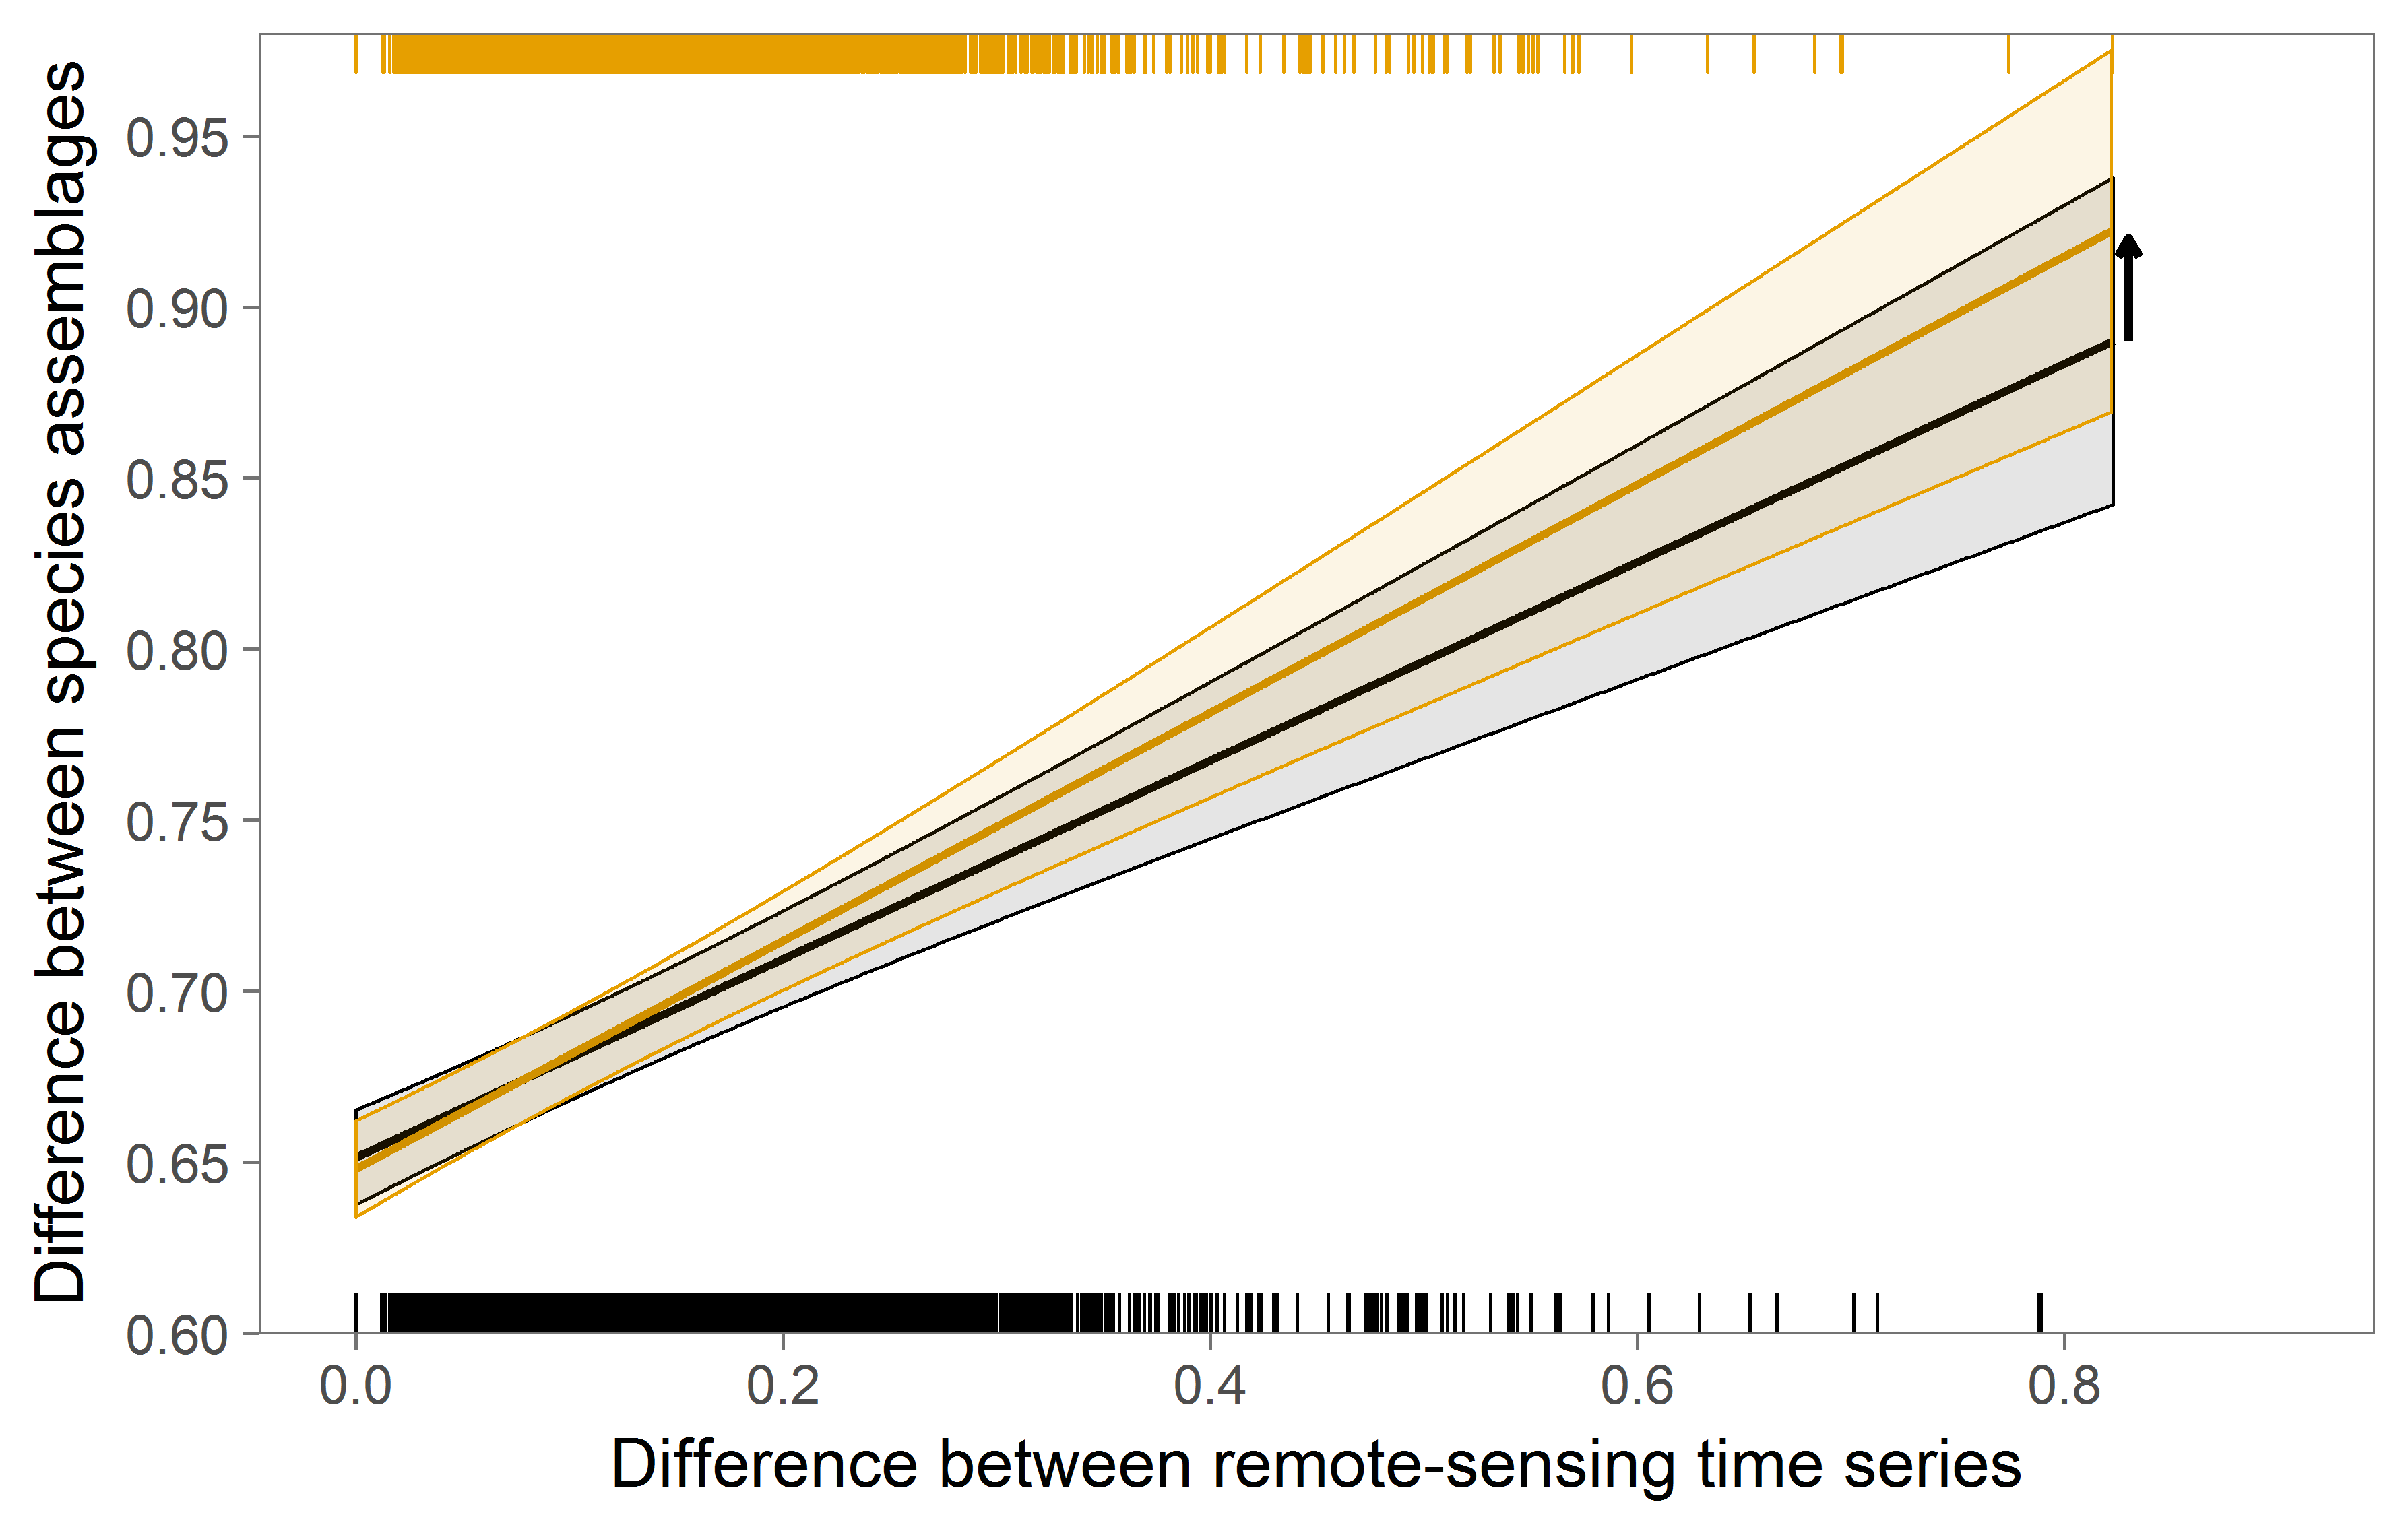
\includegraphics[width=1\textwidth]{chapter2/F02}
\caption{Shows the estimated influence of current (black) and past (orange; assessed over the past five years) BC\textunderscript{EVI} on differences in species assemblages (N = 198 studies). Rugs show the distribution of values from a single randomly selected permutation. The difference between the slopes (arrow) is the relative influence (as ratio) shown in Figures 3-6. Shading shows the predicted standard error.}
\label{F02_02}
\end{figure}
% -------------------------------------------- %

Estimating pairwise comparisons in any regression model would imply substantial pseudo-replication. To account for this, we took the subdiagonal of 100 permuted site-by-site matrices (Appendix Figure \ref{SI02_03}) to construct the GLMMs of 100 separate permutations. This ensures that for each fitted GLMM, our pairwise comparisons are mutually independent subsets \citep{Longacre2005,Newbold2016}. Fixed effects and standard errors for both current and past BC\textunderscript{EVI} were averaged across all permutations. Furthermore, for each model we calculated a marginal and conditional pseudo R-square \citep{Nakagawa2013} and significance estimate \cite{Halekoh2014}, and averaged them across all permutations. As for the fixed effects and precision estimates, the differences in explained marginal variance of past BC\textunderscript{EVI} were assessed relative to the explained marginal variance of current BC\textunderscript{EVI}.

All analyses were performed in R \citep[ver 3.2.2]{RTeam2014} using lme4 \citep[ver. 1.10]{Bolker2009,lme4} for modelling, and vegan \citep[ver. 2.2.3]{Oksanen2015} for the BC calculation of species assemblages data. The processed MODIS data and R-code for the analyses are available on GitHub (\href{https://github.com/Martin-Jung/PastLandSurfaceConditions}{https://github.com/Martin-Jung/PastLandSurfaceConditions}). 

\section{Results}
\label{C02_03}
The compositional dissimilarity of species assemblages (BC\textunderscript{Biodiversity}) increased with between-site dissimilarity in current and past photosynthetic activity (BC\textunderscript{EVI}; current: $\beta$ = 0.289, $\beta_{SE}$ = 0.063, p < 0.001; past yr\textunderscript{1:5}: $\beta$ = 0.334, $\beta_{SE}$ = 0.07, p < 0.001; Figure \ref{F02_02}, Appendix Figure \ref{SI02_05}). When the influence of past BC\textunderscript{EVI} was assessed relative to current BC\textunderscript{EVI}, the BC\textunderscript{Biodiversity} between sites was more pronounced – although the imprecision also increased - when longer time periods (of up to five years) of past BC\textunderscript{EVI} were considered (Figure \ref{F02_03}). Furthermore, the consideration of past BC\textunderscript{EVI} calculated up to five years prior to current BC\textunderscript{EVI} increased the relative explained marginal variance by 16.7\% (Appendix Table \ref{SIT02_01}). We ensured that the BC index was robust with regards to varying time period lengths (Appendix Figure \ref{SI02_06}), spatial autocorrelation (Appendix Figure \ref{SI02_07}) and other temporal and geographic biases (Appendix Figure \ref{SI02_08}). Similar results were found by using a different metric of species assemblage composition, the S\o rensen similarity index, that does not require species abundance estimates (Appendix Figure \ref{SI02_09}).

% ---------------- Figure 3 --------------------- %
\begin{figure}[ht]
\centering
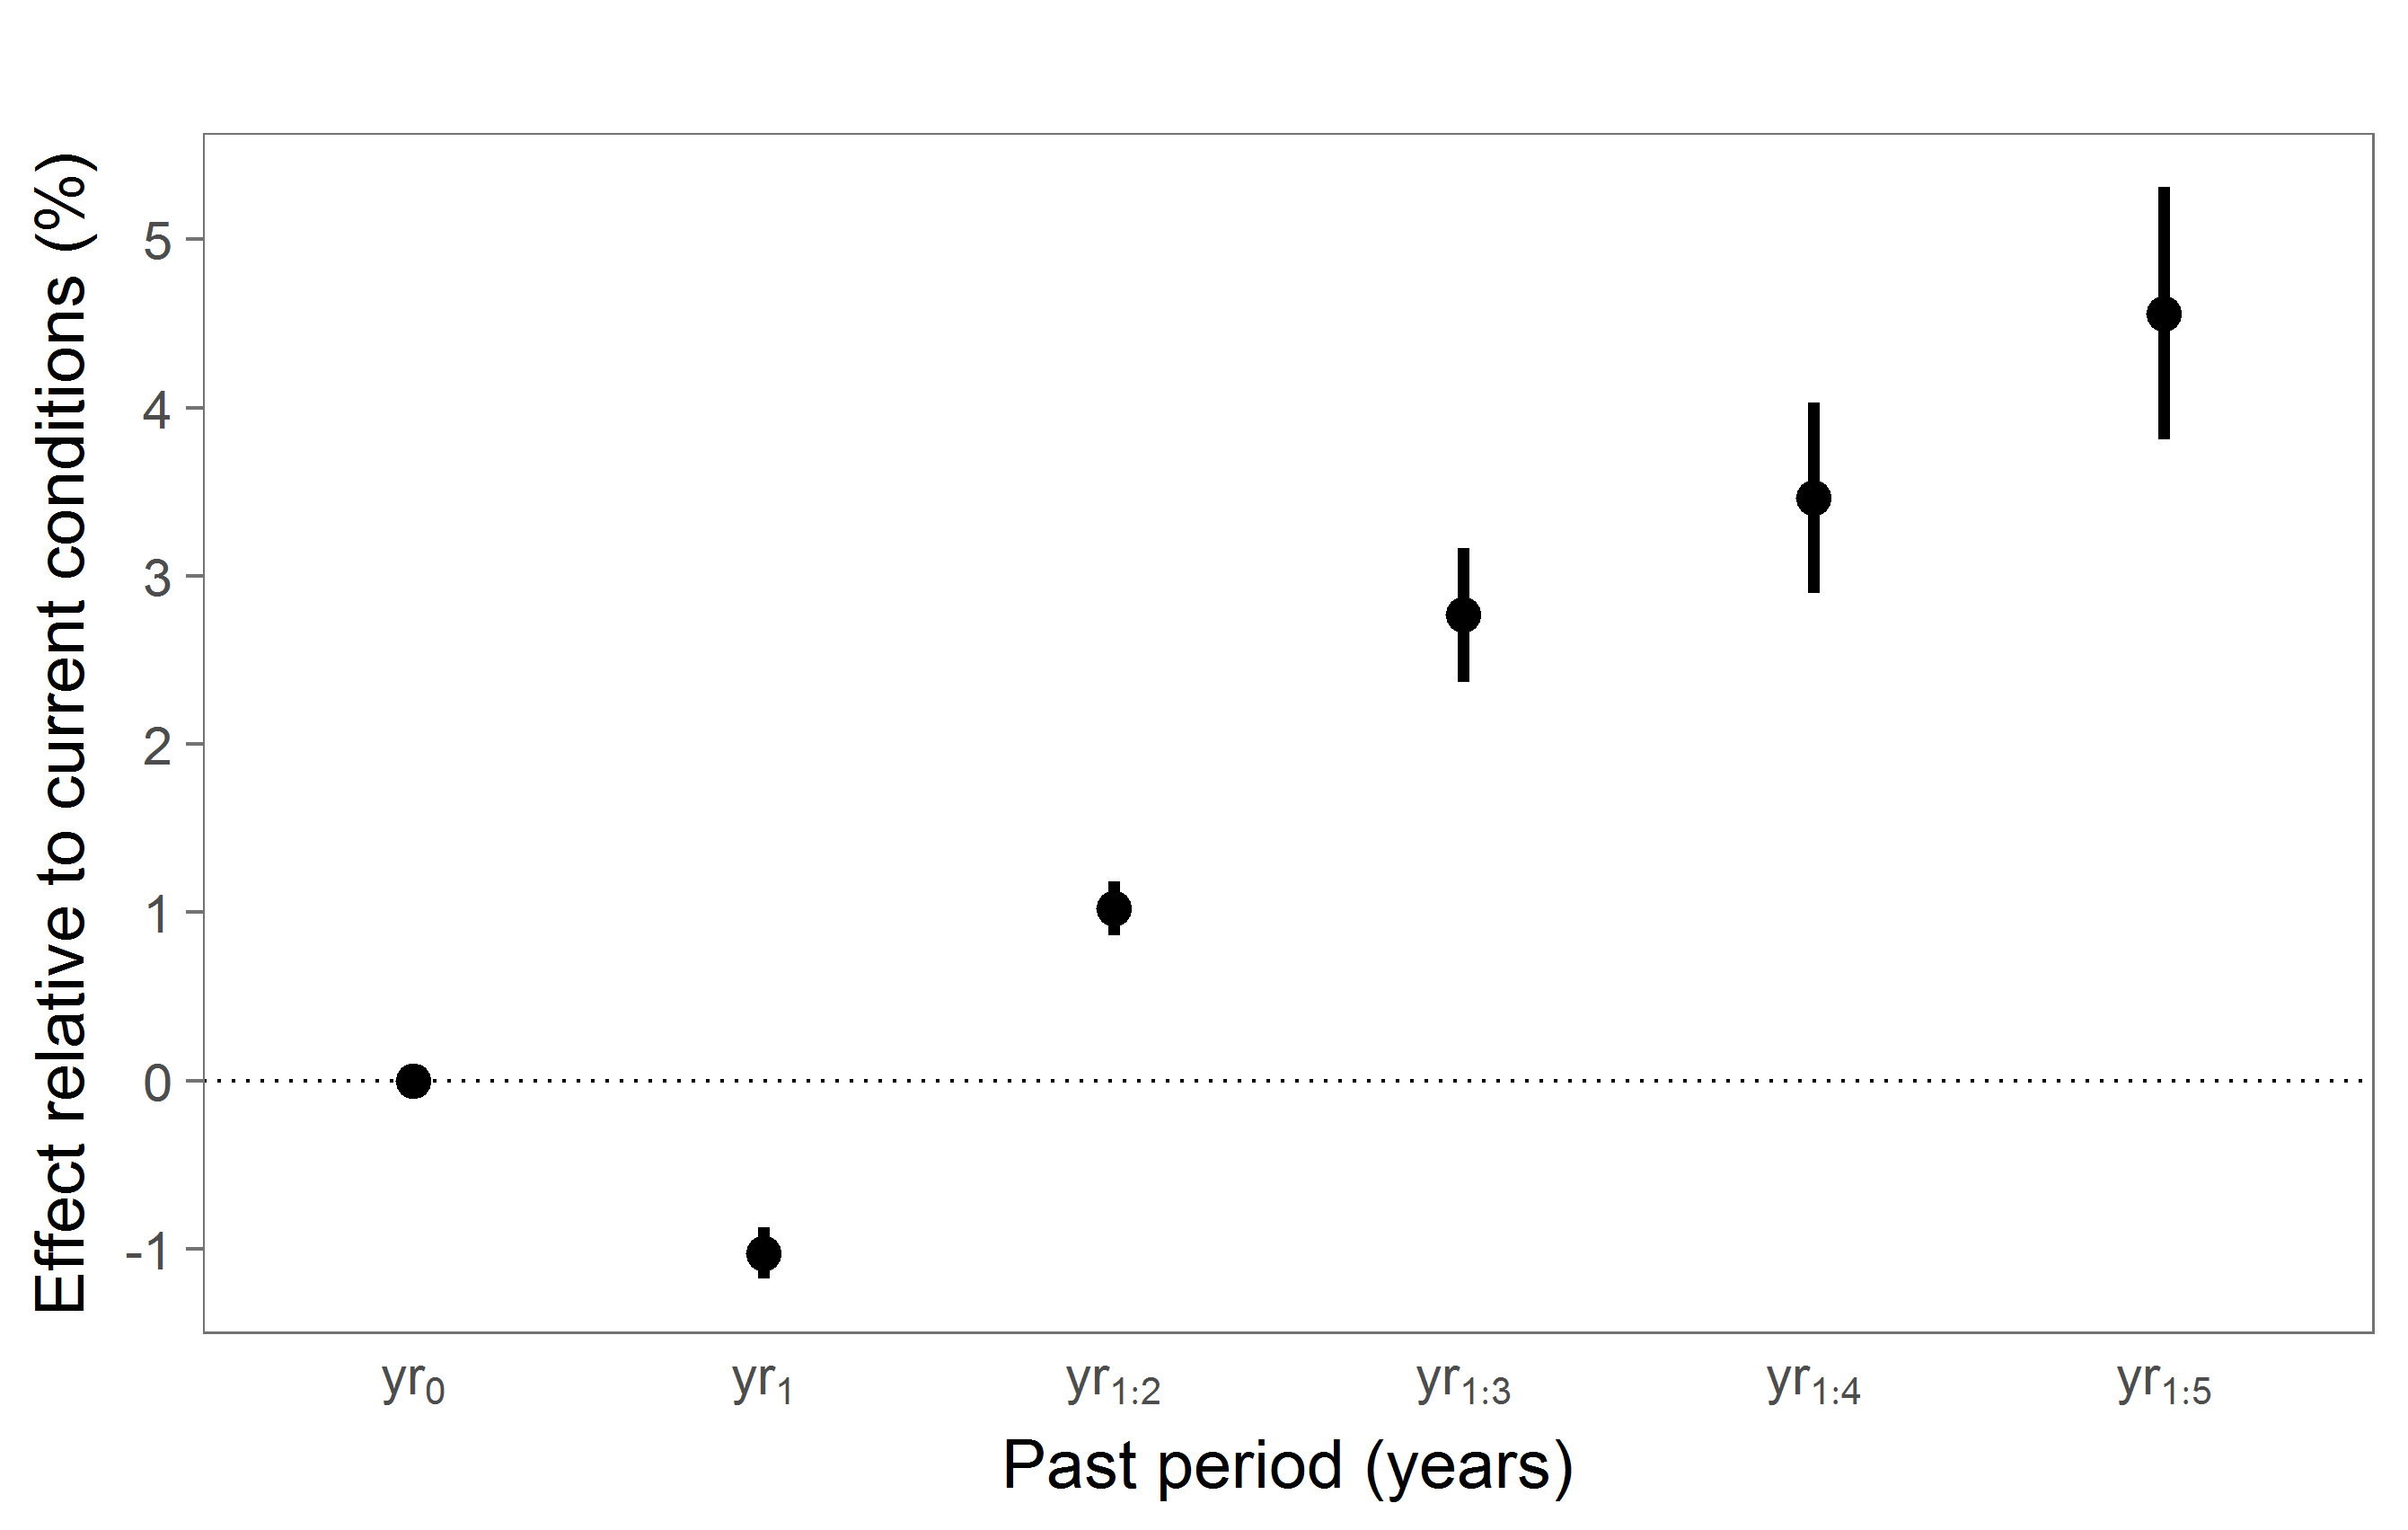
\includegraphics[width=1\textwidth]{chapter2/F03}
\caption{Overall influence on species assemblage composition of past BC\textunderscript{EVI} relative to current BC\textunderscript{EVI}, estimated individually for past periods of differing length (yr\textunderscript{1} to yr\textunderscript{1:5}, representing 1 year and up to 5 years current BC\textunderscript{EVI}). The predicted effects and their precision (standard error) of past BC\textunderscript{EVI} (yr\textunderscript{1:5}) on dissimilarity in species assemblages were transformed relative to the effects and precision of current BC\textunderscript{EVI} (yr\textunderscript{0}). Note that error bars indicate the predicted precision of differences in past BC\textunderscript{EVI} relative to the precision of differences in current BC\textunderscript{EVI}. Positive values indicate that differences in past BC\textunderscript{EVI} lead to greater differences in species assemblages than differences in current BC\textunderscript{EVI}.}
\label{F02_03}
\end{figure}
% -------------------------------------------- %
The influence of past BC\textunderscript{EVI} on species assemblages was found to vary among taxonomic groups and time periods considered (Figure \ref{F02_04}). Dissimilarity in plant, invertebrate, reptilian and bird assemblage composition increased with increasing BC\textunderscript{EVI} of the past two to five years. In contrast, the influence of past BC\textunderscript{EVI} on mammalian assemblages was greatest for the first two years relative to the influence of current BC\textunderscript{EVI} but decreased when longer periods of three to five years of past BC\textunderscript{EVI} were considered. Meanwhile, amphibian assemblages were more influenced by current than past BC\textunderscript{EVI} between sites (Figure \ref{F02_04}).
% ---------------- Figure 4 --------------------- %
\begin{figure}[ht]
\centering
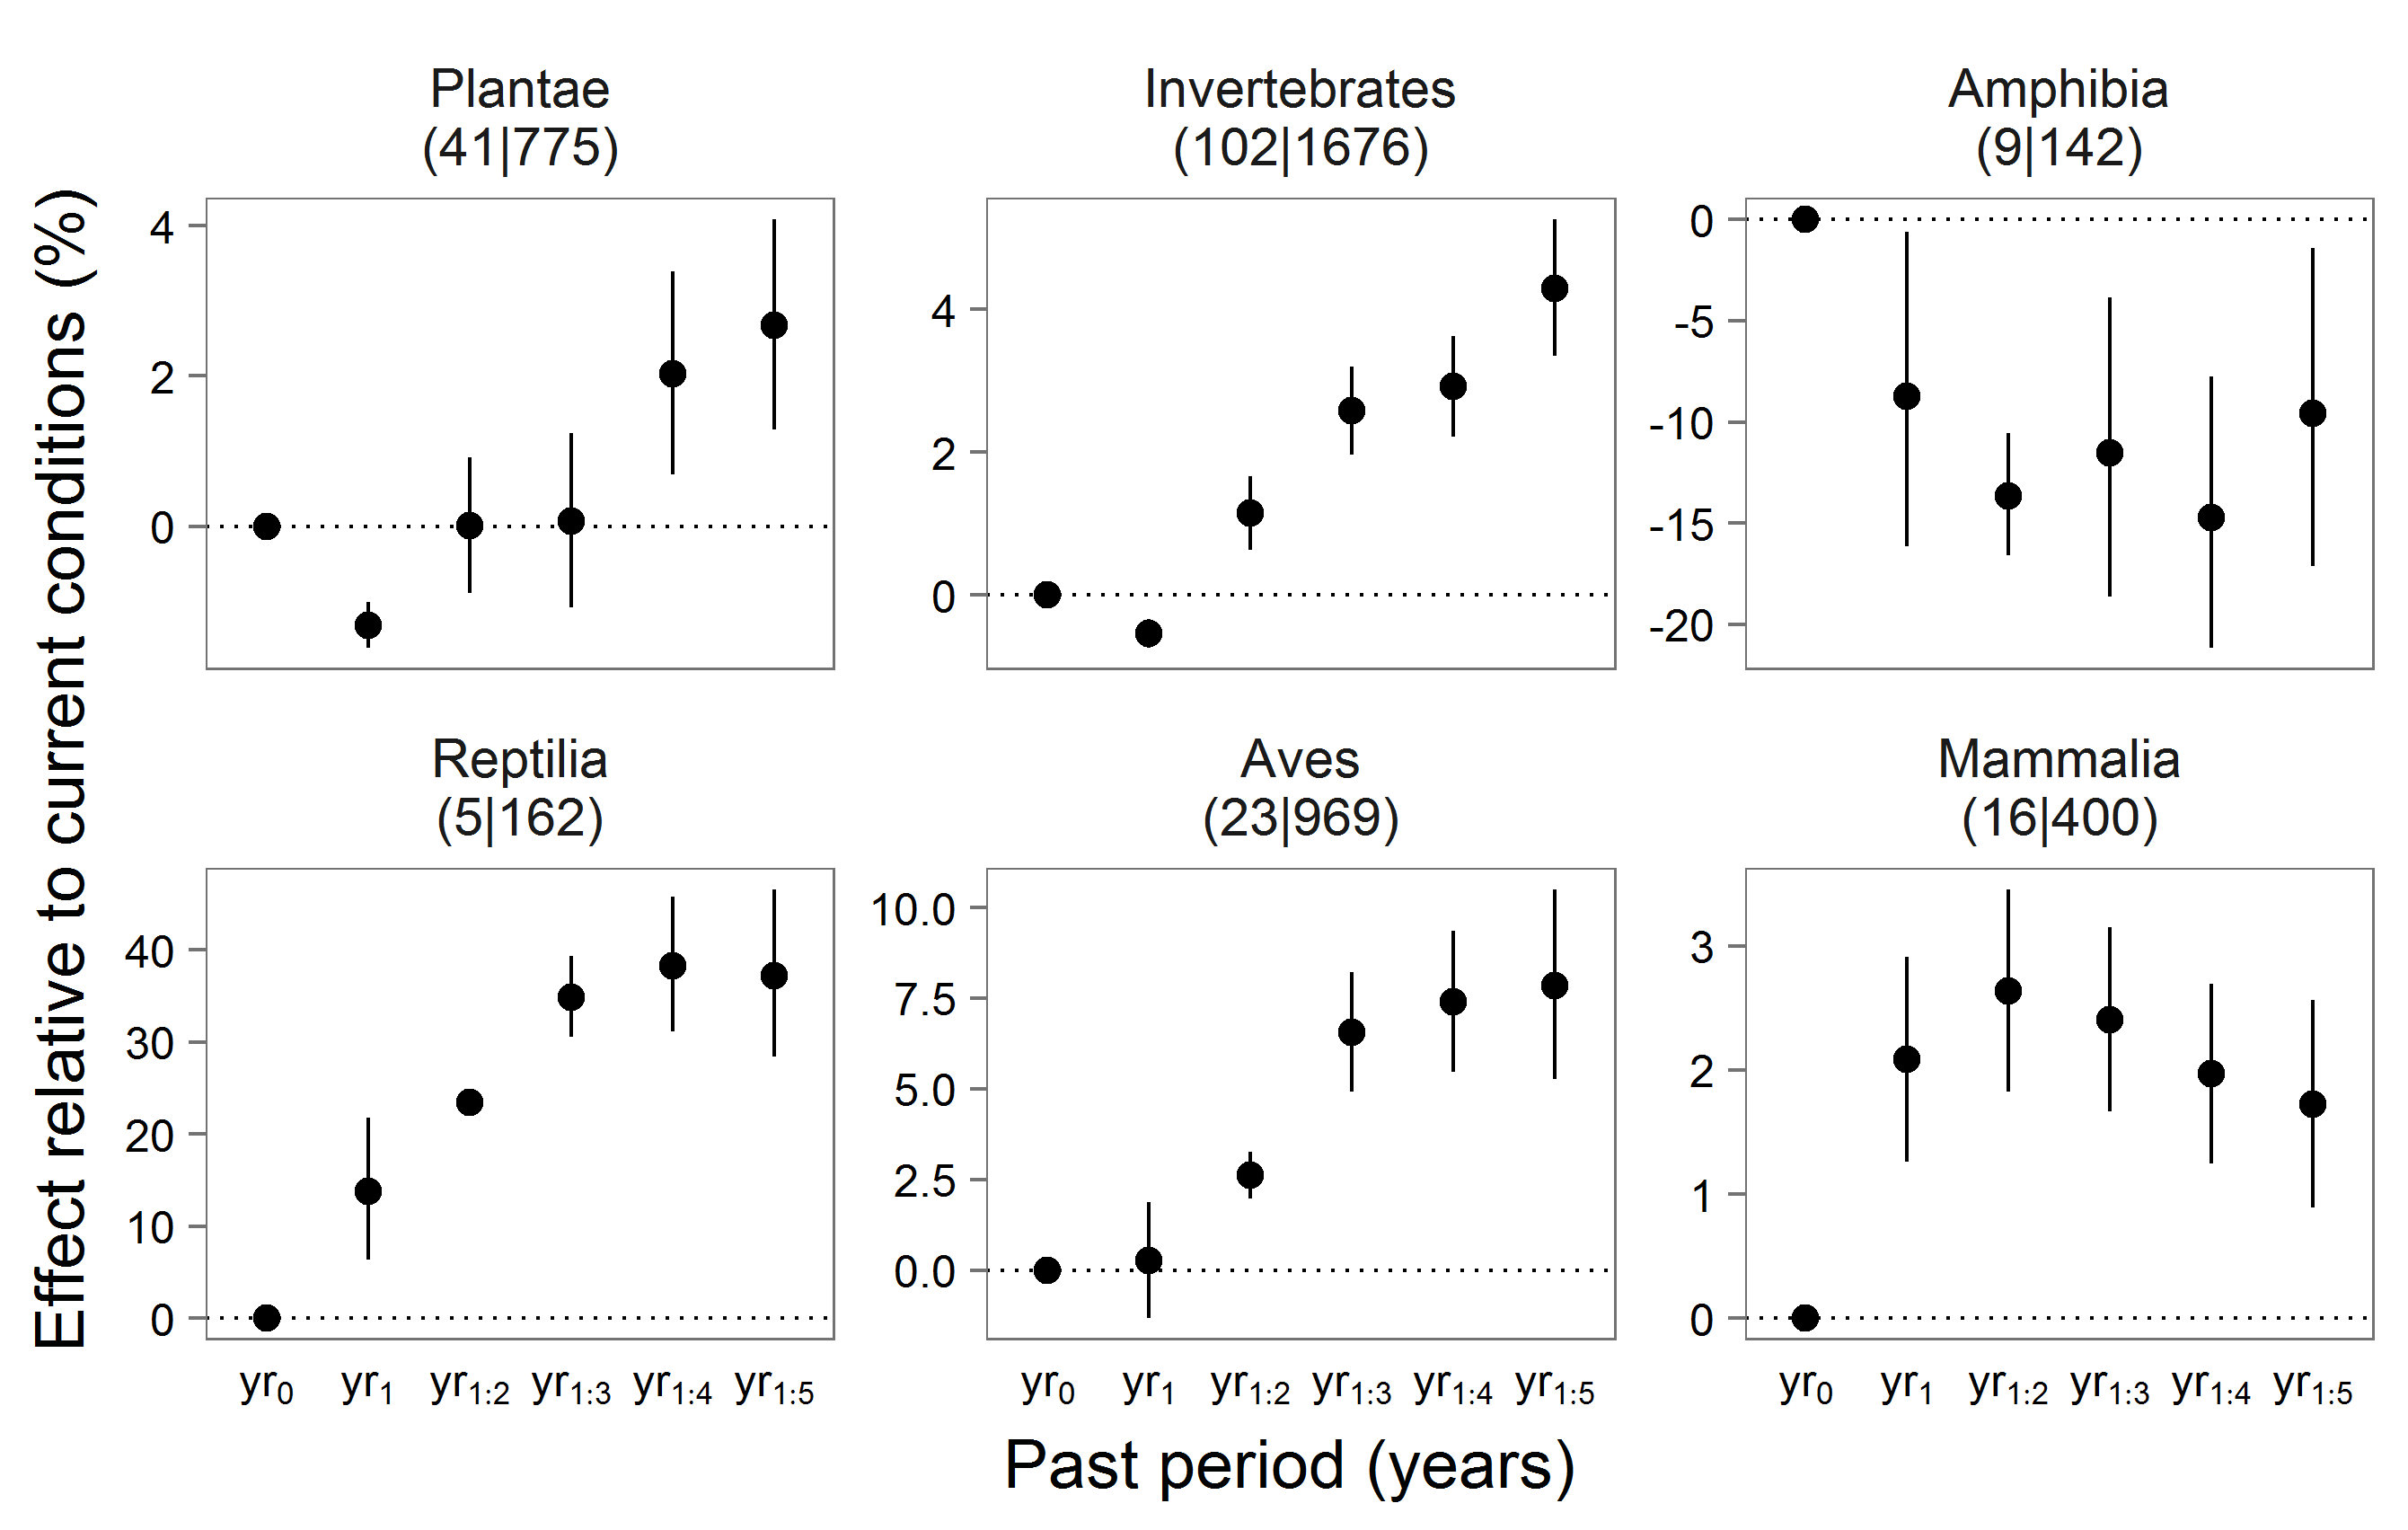
\includegraphics[width=1\textwidth]{chapter2/F04}
\caption{Influence of past BC\textunderscript{EVI} on species assemblage composition across different taxonomic groups. Visualized as relative influence of past BC\textunderscript{EVI} compared to current BC\textunderscript{EVI} as described in Figure \ref{F02_03}. The number of studies and contributing sites (N | N\textunderscript{Sites}) is indicated for each group.}
\label{F02_04}
\end{figure}
% -------------------------------------------- %
The influence of past BC\textunderscript{EVI} differed with respect to body size (Figure \ref{F02_05}). Species assemblages that were dominated by small- (> 0-9 g body mass) and medium-sized (10-99 g) mammals were more influenced by differences in BC\textunderscript{EVI} over the past one to three years, while the influence on assemblages dominated by larger ($\geq$ 100 g) mammals increased with longer time periods. Compared to assemblages dominated by medium-sized birds, assemblages of large bird species were up to five times more influenced by past relative to current BC\textunderscript{EVI}. For plant assemblages with available information on size, we found that assemblages dominated by medium-sized plants were more influenced by past BC\textunderscript{EVI} compared to those assemblages dominated by larger plant species (Figure \ref{F02_05}). 
% ---------------- Figure 5 --------------------- %
\begin{figure}[ht]
\centering
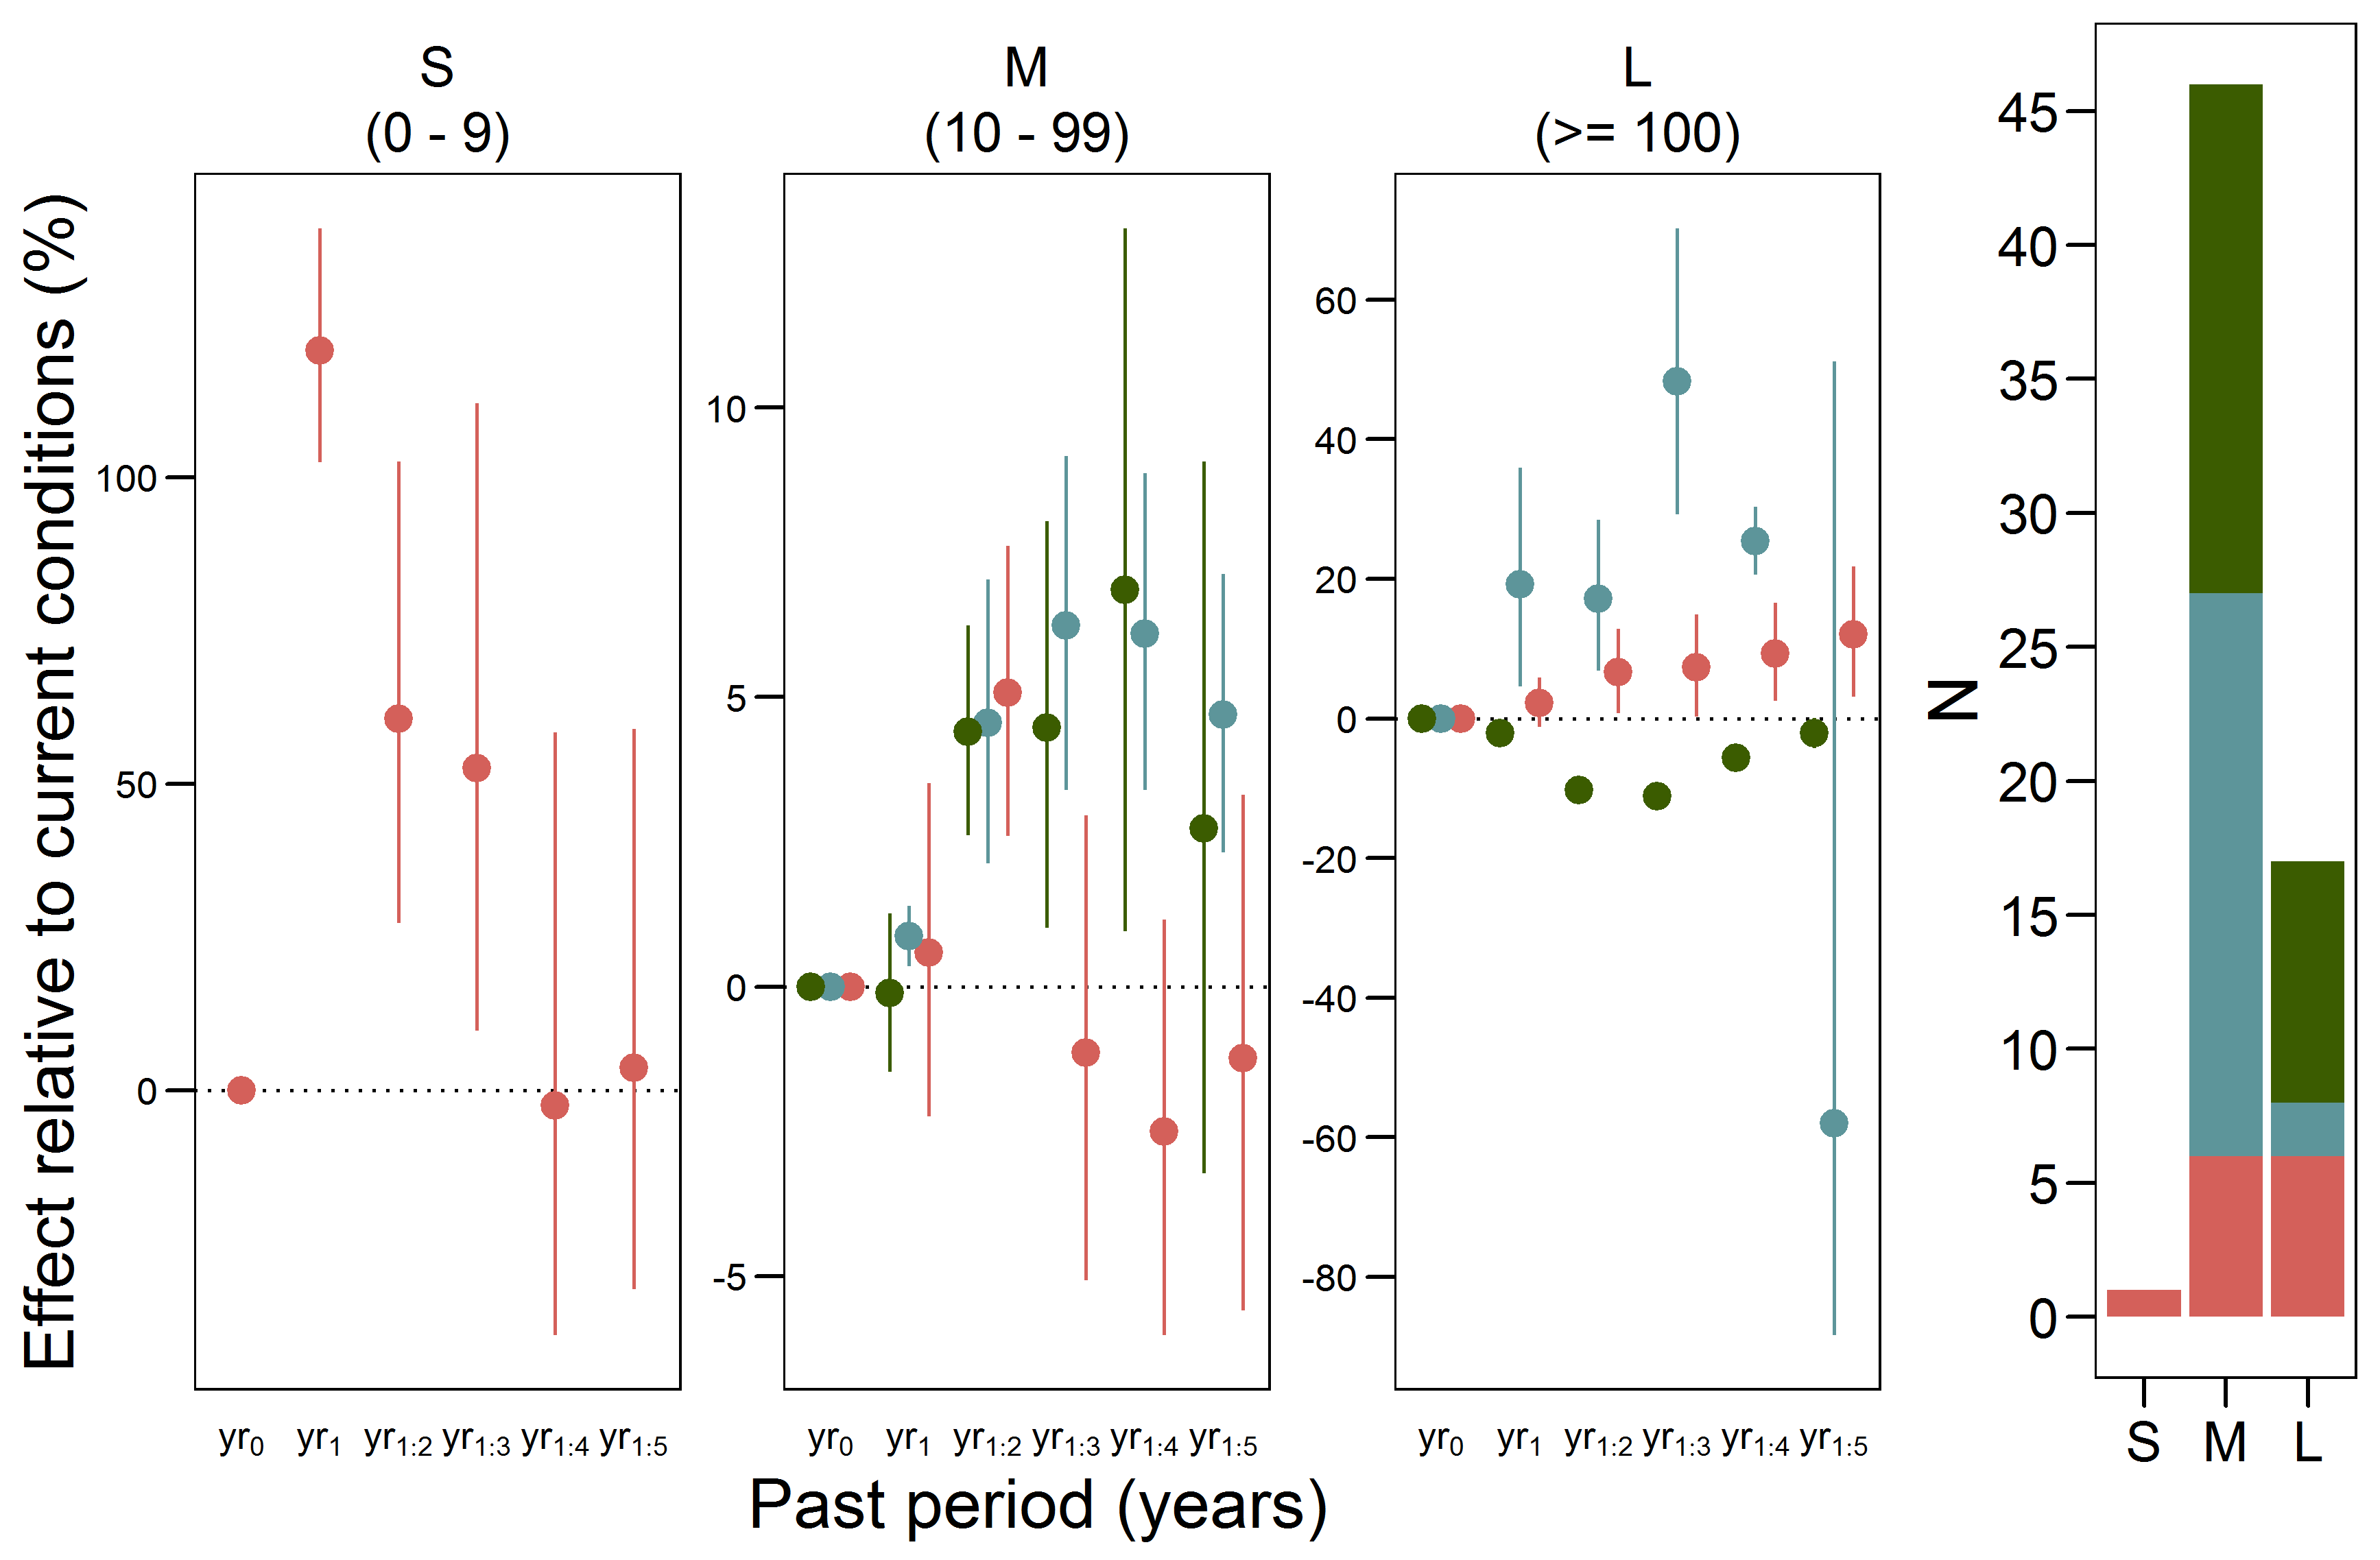
\includegraphics[width=1\textwidth]{chapter2/F05}
\caption{Influence of past BC\textunderscript{EVI} on species assemblages (N = 65) of predominantly small (> 0 - 9), medium (10 - 99) and large sized animals and plants ($\geq$ 100). Available size was measured as adult body mass (in g) for all birds (blue) and mammals (red) and height for plants (green, in cm). Within each study all species were binned into one size group and the study categorized based on which size group is predominant across all sites. The bar chart shows the number of studies that contributed to each taxonomic group and body size bin. Visualized as relative influence of past BC\textunderscript{EVI} compared to current BC\textunderscript{EVI} as described in Figure \ref{F02_03} and methods.}
\label{F02_05}
\end{figure}
% -------------------------------------------- %
Differences among trophic levels were also seen in the influence of past BC\textunderscript{EVI} on BC\textunderscript{Biodiversity} and increased with longer time periods considered (Figure \ref{F02_06}). Species assemblages dominated by omnivorous and herbivorous assemblages were more influenced by past BC\textunderscript{EVI} of even one year relative to the influence of current BC\textunderscript{EVI}, while detritivores assemblages were only more influenced by past BC\textunderscript{EVI} if periods of the past three years were considered (Figure \ref{F02_06}). In contrast, studies with predominantly carnivorous species were more influenced by current BC\textunderscript{EVI} and showed no overall trend with longer time periods of past BC\textunderscript{EVI} considered (Figure \ref{F02_06}). 
% ---------------- Figure 6 --------------------- %
\begin{figure}[ht]
\centering
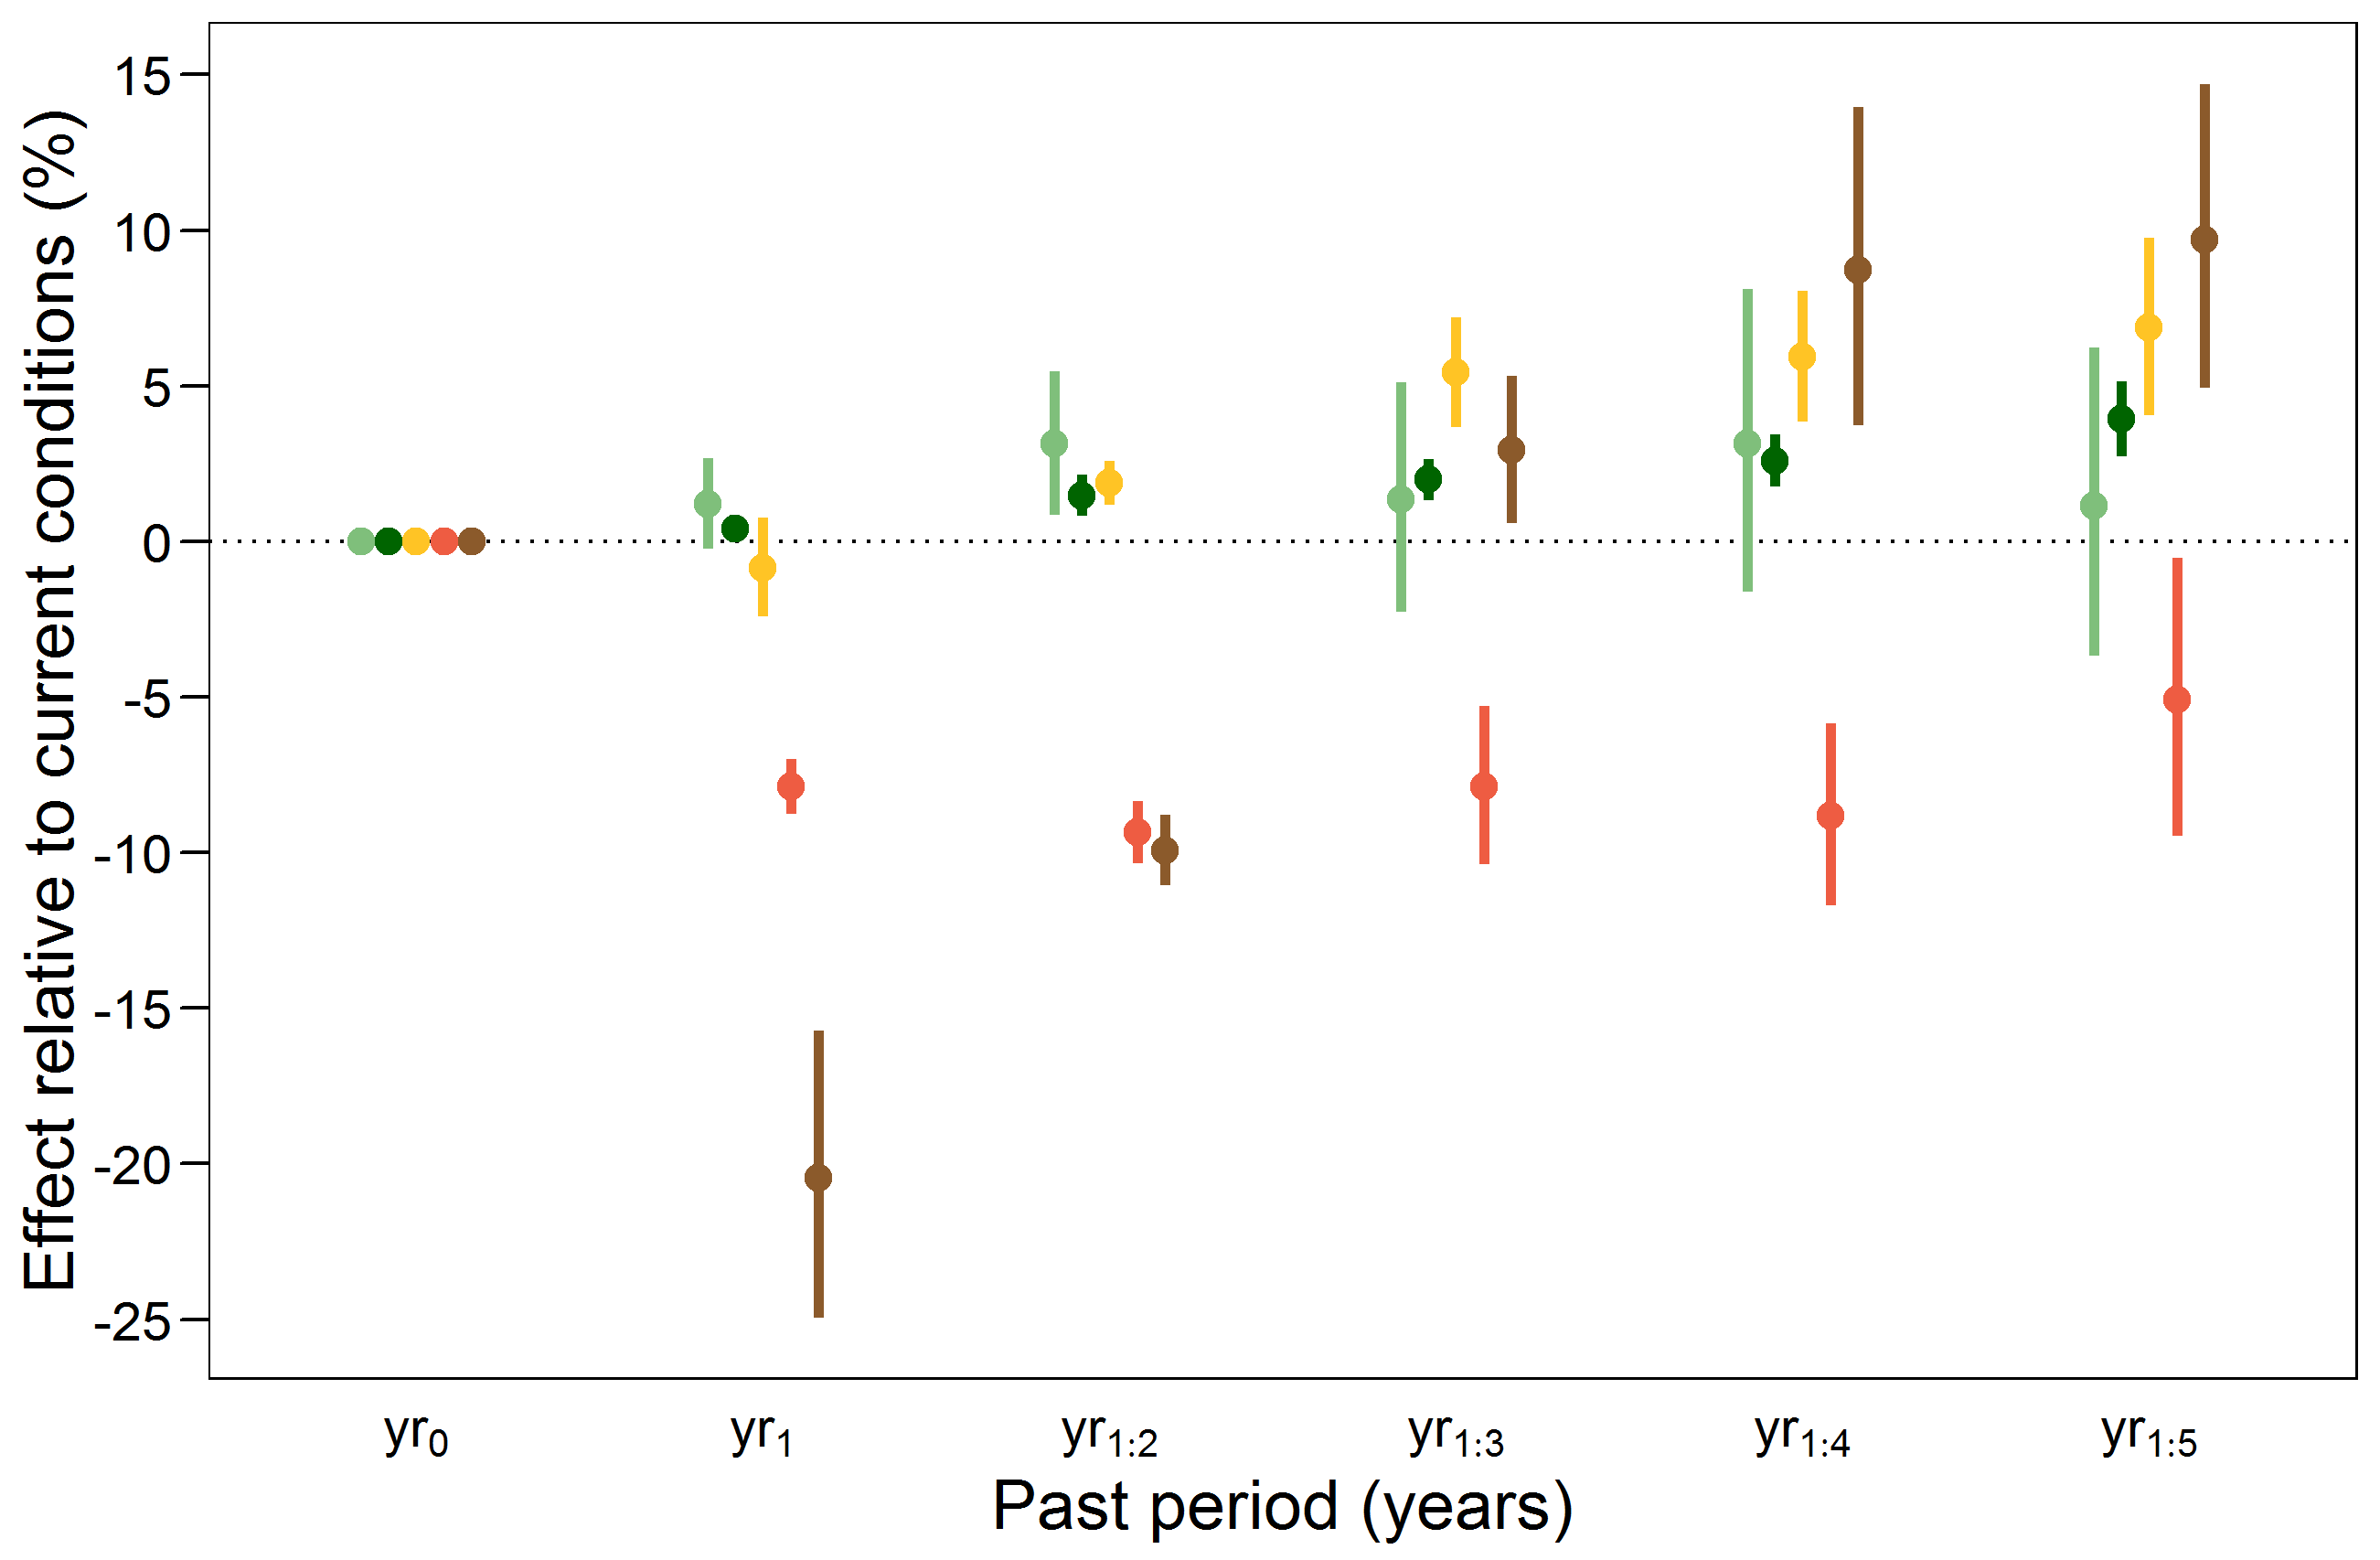
\includegraphics[width=1\textwidth]{chapter2/F06}
\caption{Influence of past BC\textunderscript{EVI} on trophic bins across studies (N = 130). Within each study all species were categorized as one trophic level and the study categorized based on which level is predominant across all sites. Colours indicate the influence of current and past BC\textunderscript{EVI} for autotroph plants (light green, N=28), herbivores (dark green, N=49), omnivores (yellow, N= 29), carnivores (red, N=13) and detritivores (brown, N=9). Visualized as relative influence of past BC\textunderscript{EVI} compared to current BC\textunderscript{EVI} as described in Figure \ref{F02_03}.}
\label{F02_06}
\end{figure}
% -------------------------------------------- %

\section{Discussion}
\label{C02_04}
The main aim of this study was to investigate if between-site dissimilarity in current and past photosynthetic activity of vegetation (BC\textunderscript{EVI}) can predict compositional dissimilarity in sites’ species assemblages (BC\textunderscript{Biodiversity}). In contrast to previous PREDICTS-based studies that used discrete measures of current land use and land-use intensity \citep{Newbold2015,Newbold2016}, we used a continuous measure of between-site dissimilarity in remotely-sensed photosynthetic activity that summarises (inter- and intra-annual) vegetation dynamics in a single metric (the BC\textunderscript{EVI}). We explicitly differentiated between current (the full year prior to species assemblage sampling) and past BC\textunderscript{EVI} (periods of up to five years before current) that could have influenced compositional dissimilarity in species assemblages. Similar to previous studies using the same dataset to analyse compositional differences with respect to land use \citep{Newbold2016}, we found that sites with more different current BC\textunderscript{EVI} also had more different species assemblages (Figure \ref{F02_02}, Appendix Figure \ref{F02_05}). However, the BC\textunderscript{EVI} calculated over five years prior to biodiversity sampling had, on average, an even greater influence on between-site dissimilarity in species assemblage composition compared to current BC\textunderscript{EVI} (Figure \ref{F02_03}). This pattern was consistent across most taxonomic (Figure \ref{F02_04}) and functional groups (Figure \ref{F02_05} and \ref{F02_06}). Here we discuss potential causes and implications of the observed patterns as well as factors that can affect the BC\textunderscript{EVI}.

\subsection{Potential drivers of dissimilarities in photosynthetic activity}
\label{C02_0401}
Dissimilarities in photosynthetic activity can be caused by many natural \citep{Fensholt2012,Zhu2016} and/or anthropogenic factors \citep{Lambin2006,Turner2007}. The latter were likely the dominant cause of current differences between sites in our analyses, given that the PREDICTS database includes only studies of mostly small geographic extent with a difference in current human land use or land-use intensity \citep{Hudson2016}, however climatic factors likely influence the BC\textunderscript{EVI} as well. Dissimilarity metrics of photosynthetic activity can be considered a coarse approximation of overall differences in land use and land cover as well as in climatic and other abiotic factors between sites \citep{Linderman2005,Lupo2007,Lhermitte2011}. Past studies have linked differences in vegetation dynamics with the use intensity of agriculture \citep{Estel2015,Tong2017}, land-cover change such as deforestation events  \citep{Lambin1994,DeVries2015b}, or land degradation and intensification \citep{DeJong2011,Muller2014}. The BC\textunderscript{EVI}, similar to other metrics used to monitor remotely-sensed vegetation dynamics \citep{Linderman2005,Rowhani2008,Lhermitte2011}, quantifies dissimilarity in photosynthetic activity across different types of land cover, by exploiting both distance between time series (the absolute difference in EVI data) and amount (area under the time series) of photosynthetic activity. Besides differences in land use and land cover, dissimilarity metrics such as the BC\textunderscript{EVI} will also be affected by climatic differences in precipitation and radiation \citep{Fensholt2012,Zhu2016}, soil properties \citep{Ahmed2017} or plant species composition \citep{He2009}. The BC\textunderscript{EVI} thus quantifies dissimilarity in vegetation dynamics caused by both natural and anthropogenic factors affecting EVI time-series.

However, some natural and anthropogenic factors cannot be directly quantified from remotely-sensed time series \citep{Peres2006,Turner2007} and the BC\textunderscript{EVI} is limited to those aspects that affect photosynthetic activity of vegetation. Furthermore, because of the way the BC\textunderscript{EVI} is calculated, it can only represent overall dissimilarity in photosynthetic activity but cannot be used to infer directionality or timing of change (vegetation regrowth or loss, disturbances such as fires, etc.). By using entire periods (\ie five full years, instead of the fifth year) it is not possible to disentangle overall dissimilarity and any ‘change’ in photosynthetic activity \textit{per se} \citep[cf.][]{Linderman2005}. Calculating the BC\textunderscript{EVI} index on longer time periods did not affect the possible range of observed values (Appendix Figure \ref{SI02_06}), however it likely enhances our ability to capture aspects of past variability in vegetation dynamics caused by either natural and/or anthropogenic drivers. We recommend that future studies evaluate the performance of the BC\textunderscript{EVI} relative to other time-series dissimilarity metrics. 

\subsection{Influences of current and past dissimilarities in photosynthetic activity on biodiversity}
\label{C02_0402}
Our results suggest that species assemblage composition was consistently more dissimilar between sites with greater current dissimilarity in photosynthetic activity of vegetation (as quantified by the BC\textunderscript{EVI}) (Figure \ref{F02_02}, Appendix Figure \ref{F02_05}). This is in line with previous studies that have correlated some measurement of dissimilarity in current ‘environmental heterogeneity’ with compositional dissimilarity in species assemblage composition \citep{Buckley2008,He2009,Newbold2016}. However species assemblages might also be explicitly influenced by past dissimilarity in photosynthetic activity \citep{Johnson2008,Watson2014,Ogle2015,Perring2015}. 

Differences in past BC\textunderscript{EVI} were on average more correlated with dissimilarity in species assemblages than differences in current BC\textunderscript{EVI} (Figure \ref{F02_02}-\ref{F02_03}). This could indicate that past dissimilarity in photosynthetic activity continues to have a lasting influence or memory effect on species assemblages \citep{Ogle2015}, especially as the effect generally increased as longer periods of past BC\textunderscript{EVI} were considered (Figure \ref{F02_03}), therefore increasing the likelihood that past changes in photosynthetic activity of vegetation have been captured. Longer periods of past BC\textunderscript{EVI} also increased the explained marginal variance (Appendix Table \ref{SIT02_01}), although most of the variance was already explained by differences in study identity (thus by sampling methods and local factors). The marginal variance explained was modest, but comparable to other broad-scale studies using the same species assemblage dataset \citep{Newbold2014b,DePalma2015,Jung2016}. It is a limitation that we used data from a wide variety of sources \citep{Hudson2016}, which were typically not designed to study lag or memory effects of past changes in land-surface conditions such as photosynthetic activity. At many of the sites in our analyses inter-annual photosynthetic activity could have remained relatively stable during the past five years, which would reduce our ability to differentiate any effects of past BC\textunderscript{EVI}. Similarly, any dissimilarity in photosynthetic activity among pairs of sites could have been even greater before the monitoring period of MODIS (since year 2000), which we were unable to quantify using these data. 

Notably, species assemblages of some taxonomic groups were more dissimilar in composition than others if past dissimilarity in photosynthetic activity was considered (Figure \ref{F02_04}). The influence of past BC\textunderscript{EVI} on reptilian species assemblages was large (\textasciitilde35\% more different than current) even for the relatively short period of five years (Figure \ref{F02_04}). Potentially many of the sites of the reptilian studies have been subjected to relatively recent changes in photosynthetic activity of vegetation prior to species assemblage sampling. Indeed, in one of the studies, \cite{Woinarski2009} explicitly suggested an influence of past fires and varying grazing intensity on reptilian species assemblages. In contrast, we found that amphibian species assemblages were less influenced by past compared to current BC\textunderscript{EVI}, despite being more influenced by current BC\textunderscript{EVI} than all other taxonomic groups (Appendix Figure \ref{F02_05}). An explanation could be that most compositional differences between amphibian assemblages that are attributable to past dissimilarities in photosynthetic activity are already explained by current dissimilarity in BC\textunderscript{EVI}. It may be that amphibian assemblages are more influenced by factors other than past photosynthetic activity (such as microclimatic conditions). Disentangling broad taxonomic groups into functional groups may assist in highlighting specific responses to past dissimilarities in photosynthetic activity.

Differences in functional traits can influence species responses to dissimilarity in photosynthetic activity \citep{Newbold2013,DePalma2015} and we expect that on average smaller species would be more affected by recent dissimilarity in photosynthetic activity (a few years before sampling). Our results confirm this assumption as species assemblages with predominantly small- or medium-sized plants, birds and mammals were relatively more influenced by past BC\textunderscript{EVI} over two to three years prior to sampling than by current BC\textunderscript{EVI} (Figure \ref{F02_05}). Smaller species tend to live shorter lives and disperse less far than larger species \citep{Brown2004,Thomson2011,Stevens2014}, which might make them more susceptible to dissimilarity in photosynthetic activity shortly before sampling \citep{Watson2014}. Similar to previous studies \citep{Jakovac2016} we showed that smaller plant species were more influenced by past dissimilarity in photosynthetic activity over up to five years prior to sampling as quantified by the BC\textunderscript{EVI} (Figure \ref{F02_05}). For assemblages dominated by larger plants we did not detect such an influence and it is likely that the considered period (five years) was too short to show measurable influences. Overall our results indicate that assemblages dominated by smaller species might have been more influenced by past dissimilarity in photosynthetic activity,  possibly because of carry-over or ecological memory effects \citep{Harrison2011,Ogle2015}. Other functional traits, such as generation time or dispersal capability \citep{Watson2014}, as well as better coverage of existing traits for underrepresented taxonomic groups could assist in further disentangling these influences especially given the large uncertainty across most influences (Figure \ref{F02_05}). 

The response of species assemblages to dissimilarities in past photosynthetic activity also differed between trophic bins. Except for carnivores, species assemblage composition of all trophic bins were on average more influenced by longer periods of past rather than by current dissimilarity in photosynthetic activity, as measured by BC\textunderscript{EVI} (Figure \ref{F02_06}). Yet we found noticeable lags in the observed influence of past BC\textunderscript{EVI} with varying time periods. Relative to the influence of current BC\textunderscript{EVI}, the influence of past BC\textunderscript{EVI} was larger for assemblages dominated by autotrophs, herbivores, omnivores and detritivores (Figure \ref{F02_06}). Notably, detritivores were more correlated with past BC\textunderscript{EVI} only if past periods of three to four years were considered. This supports previous studies which have shown that plant-dependant species are highly sensitive to variability in current and past photosynthetic activity as quantified by remote sensing \citep{Pettorelli2006,Newton2014}. In contrast, we found predominantly carnivorous assemblages to be less influenced by past BC\textunderscript{EVI} compared to current BC\textunderscript{EVI} regardless of the considered time period. Possibly, carnivore abundance was more influenced by contemporary prey density \citep{Terborgh2015} than past dissimilarity in photosynthetic activity (Figure \ref{F02_06}). Because of a lack of data for carnivores and herbivores co-occurring at the same site, we were unable to investigate such interactions. 

\section{Study implications and conclusions}
\label{C02_05}
Knowledge about past dissimilarities in land-surface conditions, such as photosynthetic activity, and their influence on species assemblages is important for both the design of ecological studies and interpretation of dissimilarities in current composition of species assemblages. We found that sites with more dissimilar past than current photosynthetic activity (as quantified by the BC\textunderscript{EVI}) were more strongly correlated with compositional dissimilarity in local species assemblages among spatial pairs of nearby sites. Ignoring such past influences can lead to biased biodiversity estimates by not accounting for extinction debts or immigration credits still to be paid \citep[see ][]{Tilman1994} or lasting ecological memory and carry-over effects because of higher variability in past photosynthetic activity \citep{Rowhani2008,Cole2015,Ogle2015}. We suggest that future broad scale studies investigating biodiversity responses to environmental changes should explicitly consider legacy effects that influence species assemblages in a study area and we demonstrate how remote sensing can help to quantify such effects globally. Our approach could be extended to incorporate differences in the vegetation dynamics of the surrounding landscape. There is some evidence that landscape-wide temporal differences in photosynthetic activity can affect species assemblage composition in the wider landscape \citep{Manning2009,Fernandez2016}. In conclusion, we have demonstrated that compositional dissimilarity of species assemblages, of various taxonomic and functional groups, are not only influenced by dissimilarity in current photosynthetic activity, but also by dissimilarity in past photosynthetic activity over the last five years. Future studies should investigate the influence of disturbance events and directionality of changes in photosynthetic activity for more than five years before local biodiversity sampling.

%\section{Acknowledgements}
%\label{C02_06}
%We thank all PREDICTS data contributors for their biodiversity data, which was collated using support from the Natural Environment Research Council (NERC, grant number: NE/J011193/2). PREDICTS is endorsed by the GEO BON. This study has benefited from publicly available data from the TRY initiative on plant traits (\href{http://www.try-db.org}{http://www.try-db.org}). We acknowledge the University of Sussex, School of Life Sciences for a doctoral training grant and for providing computing facilities.

\section{Data availability}
\label{C02_06}
Extracted MODIS data and pairwise biodiversity permutations are available on GitHub. A 2016 snapshot of the PREDICTS database has been openly released earlier (\href{http://dx.doi.org/10.5519/0066354}{http://dx.doi.org/10.5519/0066354}).

\clearpage
%\bibliography{content/01Chapter}

%\appendix
%\begingroup
%  Blank

%\endgroup
 % Pairwise piece
  \chapter{Impacts of past abrupt land change on local biodiversity globally}
%\addcontentsline{toc}{chapter}{Chapter 3}
%\markboth{}{Impacts of past abrupt land change on local biodiversity globally}
\label{C03}
Abrupt land change, such as deforestation or agricultural intensification, is a key driver of biodiversity change. Following abrupt land change, local biodiversity often continues to be influenced through biotic lag effects. However, understanding of how terrestrial biodiversity is impacted by past abrupt land changes is incomplete. By combining geographically- and taxonomically-broad data on local biodiversity with quantitative estimates of abrupt land change detected within time series of satellite imagery from 1982 to 2015, here we show that abrupt land change in the past continues to influence present species assemblages globally. Species richness and abundance were reduced by 4.2\% and 2\%, respectively, and assemblage composition was altered at sites with an abrupt land change compared to unchanged sites, although impacts differed among taxonomic groups. Biodiversity recovered to levels comparable to unchanged sites after >10 years. Ignoring delayed impacts of abrupt land changes likely results in incomplete assessments of biodiversity change.

\section{Introduction}
\label{C03_01}
Natural and anthropogenic processes change the terrestrial surface of the Earth \citep{Ellis2013,Song2018}, which have been shown to impact biodiversity \citep{Newbold2015,Jung2018} and ecosystem services \citep{Isbell2015}. Previous studies have found that present differences in land-surface conditions reduce local biodiversity globally \citep{Gibson2011,Newbold2015}. However, these studies often ignore the impacts of past land change \citep{Foster2003,Watson2014}. Simulations and experiments have demonstrated that land changes of greater magnitude have larger impacts on the number of species and individuals \citep{Dornelas2010,Hautier2015,Santini2016}. Yet, few studies have quantified the impacts of land change in the past on local biodiversity globally.

Local biodiversity continues to be influenced by past land change through biotic lags. Biotic lags—including ecological processes such as extinction debt \citep{Tilman1994,Kuussaari2009,Halley2016}, colonization credit \citep{Hylander2013} and ecological memory effects \citep{Ogle2015}—negatively affect the number of species and individuals present within local assemblages \citep{Halley2016,Jung2018,Perring2018}, and potentially reduce resilience \citep{Hautier2015,Nimmo2015}. The impacts of land change on species assemblages through biotic lag depend on species’ abilities to persist \citep{Turner1998} and recover \citep{Martin2013,Fu2017,Moreno-Mateos2017}. Most previous global studies \citep{Supp2014,Fu2017,Moreno-Mateos2017,Shackelford2017} investigating abrupt land changes in the past have used descriptive study-specific categories of “land changes”, \eg wild fire, flooding or cultivation, thus hindering comparisons among studies, and preventing predictions. To assess the impacts of abrupt land change on local biodiversity more generally, comparable quantitative measures of “land change” are needed.

The availability of time series of satellite imagery enables the detection and quantification of land changes globally \citep{Kennedy2014,Song2018}. Land change can be defined as abrupt shifts in intra- and inter-annual dynamics of remotely-sensed photosynthetic activity quantified through vegetation indices \citep{Linderman2005,Pettorelli2005}. Abrupt shifts in magnitude \citep{Kennedy2012,Watson2014,DeVries2015b} and/or trend \citep{dejong2013} of photosynthetic activity, and the time passed since such shifts \citep{POTTER2003,Kennedy2012} are three key attributes of land change \citep{Watson2014}. Several algorithms have been developed to detect abrupt land change \citep{Zhu2017} and measure these attributes. However, attributes of remotely-sensed abrupt land change have never before been used to assess biotic lags in local biodiversity.

Here we investigate the impacts of abrupt land change in the past—defined as the single largest shift in magnitude and/or trend of photosynthetic activity \citep{Verbesselt2010a,dejong2013,Song2018}—on local biodiversity globally. We used data on local biodiversity of unprecedented geographic and taxonomic coverage from the Projecting Response of Ecological Diversity in Changing Terrestrial Systems (PREDICTS) database \citep{Hudson2016}. At each site, where local biodiversity was sampled, we assessed time series of high spatial resolution (nominal \textasciitilde30m) Landsat satellite imagery from 1982-2015 for the presence of an abrupt land change (Figure \ref{F03_01}\textbf{a}) and, where detected, we quantified key attributes, \ie, shifts in magnitude, trend and time passed. Using hierarchical analyses, we compared four measures of local biodiversity (species richness, total abundance, evenness and species turnover) between paired sites (5,563 sites with and 10,102 without an abrupt land change) from 377 studies (Figure \ref{F03_01}\textbf{b}). We expect that abrupt land changes with larger shifts in magnitude and trend have greater impacts on local biodiversity through biotic lag effects and that with more time passed local biodiversity can recover from the impacts of abrupt land change.

% ---------------- Figure 1 --------------------- %
\begin{figure}[!htb]
\centering
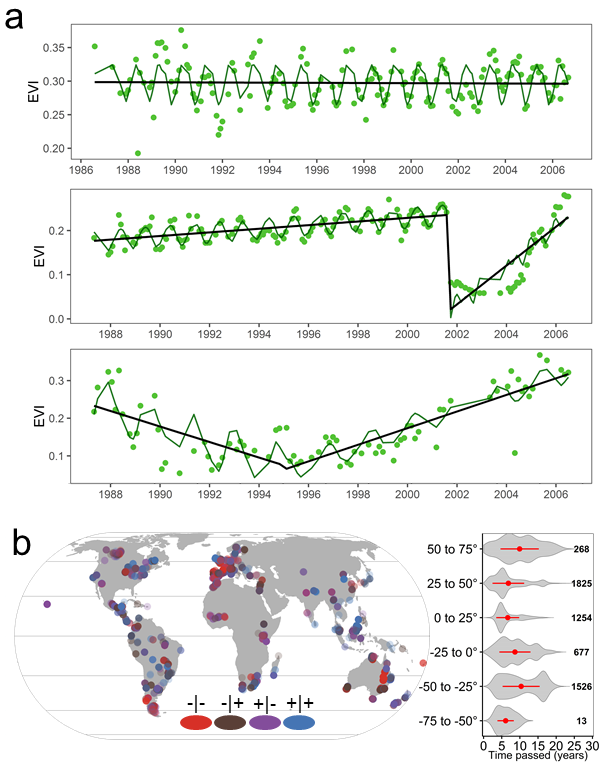
\includegraphics[width=1\textwidth]{chapter3/F01}
\caption{ Examples and distribution of sites without and with abrupt land change. (\textbf{a}) Remotely-sensed time series of monthly Enhanced Vegetation Index (EVI; green points) at an unchanged site; a site with an abrupt shift in magnitude, \ie, loss in EVI; and a site with a shift in EVI trend, \ie, an increase in annual EVI. Linear (black lines) and seasonal (dark green lines) fits of the change detection algorithm \citep{Verbesselt2010a} are shown. (\textbf{b}) Location of 5,563 sites from 377 studies in the PREDICTS database with an abrupt land change in the monitoring period (since 1982) of the Landsat 4-8 missions. Colours indicate sites with abrupt land change that had a magnitude gain (\textbf{+}) or loss (\textbf{-}) and/or trend increase (\textbf{+}) or decrease (\textbf{-}); (magnitude | trend). For ease of viewing, the location of 10,102 sites without an abrupt land change has been omitted. Latitudinal distribution of sites with an abrupt land change and time passed between abrupt land change and biodiversity sampling (in years, mean and standard deviation shown in red) by 25\textdegree  latitudinal bands. Map shown in Eckert IV equal-area projection.}
\label{F03_01}
\end{figure}
% -------------------------------------------- %
\clearpage %so that Figure 1 appears here

\section{Methods}
\label{C03_02}
\subsection{Biodiversity data} 
\label{C03_0201}
We used data from the Projecting Responses of Ecological Diversity In Changing Terrestrial Systems (PREDICTS) database \citep{Hudson2016}, which includes species’ presence and abundance data from ‘studies’ with at least two spatially-explicit ‘sites’, information on the date of sampling, and local land-use and/or land-use intensity \citep{Hudson2016}. We simplified the original PREDICTS land use and land-use intensity information \citep{Hudson2014,Hudson2016} by allocating each site to one of three broad land-use categories: primary vegetation (\textbf{PV}, \ie primary [non-] forest), secondary vegetation (\textbf{SV}, \ie mature, intermediate, young and indeterminate age secondary vegetation) or human-dominated vegetation (\textbf{HDV}, \ie, plantation forest, cropland, pasture, urban). Studies were grouped into eight broad taxonomic groups based on the sampled taxa: plants, fungi, ground dwelling invertebrates (\eg, soil-fauna, snails, beetles), flying invertebrates (\eg, butterflies, bees, dragonflies), amphibians, reptiles, birds or mammals. 

We assessed four measures of local biodiversity that complement each other and have previously been shown to be sensitive to abrupt land change \citep{Supp2014,Santini2016}. For each site in the PREDICTS database, we calculated within-sample species richness and, where data on abundance were available, log\textunderscript{10} total abundance of individuals, adjusted by sampling effort following \cite{Newbold2014b}. After visual inspection, we removed one outlier study (a study of soil biomass, ID = \\ \detokenize{DL1_2012__CalvinoCancela}) from further analyses because of very large abundance estimates ($> 3\times 10$ \textsuperscript{6} individuals). As a measure of assemblage evenness, we calculated the arcsine square root transformed probability of an interspecific encounter (PIE), which quantifies the probability of two individuals randomly chosen from an assemblage representing different species \citep{Hurlbert1971}. As a measure of turnover in species assemblage composition within studies, we calculated the S\o rensen similarity index among spatial pairs of sites within each study and land-use category \citep{Magurran2004}.

Species assemblages were sampled at various spatial extents defined by each study’s sampling method and land use. Following the PREDICTS data curation protocol we assumed the allocated land use to be dominant within the reported sampling extent (maximum linear extent [MLE], in meters) of each site \citep{Hudson2014,Hudson2016}. For studies without reported MLE (4779 sites, 18.3\% of all sites), we used either the mean MLE for each taxonomic group and corresponding sampling method, \eg, mist netting, pitfall trapping, or the mean MLE within the same taxonomic group. To test whether these interpolated MLEs are consistent among taxonomic groups and sampling method, we randomly removed 25\% of the reported MLEs and found the interpolated MLEs to be reasonably correlated (Pearson’s r = 0.73, p < 0.001). We included all studies with a MLE < 3000m (98.3\% of all sites), approximately 100 times the nominal resolution (\textasciitilde 30m) of the remotely-sensed data used in this study, and removed four studies with sites located in water (rivers, coastal areas or ponds), identified by intersecting all sites with a global permanent water surface mask \citep{Pekel2016}, as a precaution as sites within these studies likely have low positional accuracy. To spatially link species assemblage with remote sensing data, we calculated a rectangular buffer with MLE as radius (MLE\textunderscript{mean}= 412.1 m $pm$ 1,661.82m SD) around each site’s coordinates as the smallest area that fully captures all grid cells of varying sampling units (\eg, point counts, line transects). 

\subsection{Remote sensing data} 
\label{C03_0202}
We used land-surface reflectance products derived from the sensors of the Landsat 4 (1982 – 1993), 5 (1984 - 2012), 7 (1999 – ongoing), and 8 (2013 – ongoing) missions available within Google Earth Engine (GEE) \citep{Gorelick2017}, based on raw United States Geological Service Landsat Collection images (Tier 1) to calculate the Enhanced Vegetation Index (EVI, as two-band version \cite{Jiang2008}) as a proxy of photosynthetic activity. We masked all cloud-covered grid cells (\textasciitilde 30 m nominal resolution) using the cloud-detection output in the ‘cfMask’ band \citep{Zhu2012} and removed occasional snow- and water-covered grid cells, \ie those with negative EVI values. All data preparation and extraction were performed within GEE \citep{Gorelick2017}.

For each Landsat image and PREDICTS site we calculated the mean EVI within the rectangular buffer ($\bar{y}$) and extracted time series of all EVI values. We removed outliers introduced by satellite sensor errors, missed cloud shadows or bad quality estimates by calculating the absolute difference of all $\bar{y}$ values from the median absolute deviation (MAD) per EVI time series \citep{Leys2013}. EVI values more than a conservative threshold of two units of deviation away from the MAD or in the top 1\% of all MAD estimates were set to NA \citep{Leys2013}. Time series of EVI data were temporally aggregated to monthly maximum value composites to ensure equal intervals between data points and to reduce the amount of noise and missing data. Because of the ongoing consolidation of the global Landsat archive \citep{Wulder2015}, there can be periods of consecutively missing data, particularly before the launch of Landsat 7 in 1999 (Appendix Figure \ref{SI03_01}\textbf{a}). To remove gaps of $\geq 5$ years of consecutively missing data, which might affect the precision of land change attribute calculations, we identified and then truncated time series to include only the years from 1999 onwards in subsequent analyses (see Appendix Figure \ref{SI03_01}\textbf{b}). In total 25,656 sites had suitable EVI time series, with an average 18.83 ($\pm$ 6.7 SD) years duration containing on average 1.82 years ($\pm$ 1.57 SD) of consecutively missing data.

\subsection{Abrupt land change detection} 
\label{C03_0203}
To identify the presence of abrupt land change and its attributes in EVI time series, we used the Breaks For Additive Season and Trend (BFAST) algorithm \citep{Verbesselt2010} modified to work with missing data and optimized to find the single most influential abrupt land change in a time series \citep{dejong2013}. BFAST accurately detects abrupt land changes \citep{Verbesselt2010a,DeVries2015b} by using a multiple regression model to estimate both trend and seasonal components of a time series \citep{dejong2013}: $ \bar{y}_t = \alpha_{s} + \beta_{s}t + \sum_{p=1}^{k} \gamma_{p}\sin (\frac{2\pi pt}{h} + \delta_{p}) + \varepsilon_{t} $, where $ \bar{y}_t$ is the mean EVI at time $t$, $s$ the segment in the time series, $\alpha_{s}$ the intercept, $\beta$ the slope (\ie, trend), $p$ and $k$ the order of the seasonal term ($k = 2$), $\gamma$ the amplitude, $\delta$ the phase and $\varepsilon$ the residual error. The expected frequency to detect an abrupt land change in a time series is determined by $h$ and, following previous studies \citep{Verbesselt2010a,Verbesselt2010}, was set as the ratio of the number of data points per year (12 months) to the total length of the individual time series (in months). Whenever the inclusion of the seasonal component caused the model to fail to converge (17\% of all fitted models), we removed the seasonal component by time series decomposition (‘stlplus’ package, \cite{Hafen2016}) prior to fitting BFAST with a trend component only. BFAST detects abrupt land change when model residuals depart significantly (p < 0.05) from a statistical boundary \citep{Zeileis2005}. To test for significant departure we used two complementary approaches \citep{Zeileis2005,Verbesselt2010a,Verbesselt2010} using first, a moving sum of residuals (MOSUM) test within the monitoring period (determined by $h$) and second, an information-theoretic approach, the Bayesian Information criterion (BIC). All BFAST models were fitted using the ‘bfast’ package (ver. 1.5.7, \cite{Verbesselt2010a}) in R (ver. 3.5, \cite{RTeam2014}).

For the single most influential abrupt land change detected in each time series, we calculated the relative shift in magnitude as the immediate change in EVI [$ \frac{(\hat{y}_{j} - \hat{y}_{j-1} )}{|\hat{y}_{j-1}|}$, where  $\hat{y}_{j}$ is the first monthly estimate of $\hat{y}$ predicted by the BFAST model after an abrupt land change has been identified and $\hat{y}_{j-1}$ the predicted estimate one month before], the difference in linear trend as increase/decrease in EVI before and after the abrupt land change ($\beta_{after}-\beta_{before}$, where $\beta_{after}$ and $\beta_{before}$ are the predicted linear trends in EVI from the BFAST model, before and after the abrupt land change), and the time passed (in months, $t_{n} - t_{j}$) between the date of the abrupt land change ($t_{j}$) and the start of biodiversity sampling ($t_{n}$). Attributes of abrupt land change were grouped into bins as follows (Appendix Figure \ref{SI03_02} and Table \ref{SIT03_01}): for shifts in magnitude (> 50\%, > 25\% and $\leq$ 50\%, and $\leq$ 25\% EVI loss or gain, Appendix Figure \ref{SI03_02}\textbf{a}), for shifts in trend (0.01, 0.05, and > 0.05 lower or higher EVI trend change, Appendix Figure \ref{SI03_02}\textbf{b}) and time passed (<5, 5-10, and >10 years ago, Appendix Figure \ref{SI03_02}\textbf{c}). The three attributes of abrupt land change were only marginally correlated among each other (mean Pearson’s |r| < 0.07, Appendix Figure \ref{SI03_03}). Sites without an abrupt land change detected by BFAST are referred to as “unchanged” sites (0) and all studies containing only unchanged sites (10,196 sites of 262 studies) were excluded from further analyses.

\subsection{Statistical analyses} 
\label{C03_0204}
We built hierarchical models comparing biodiversity measures between paired sites without and with an abrupt land change in the past. Hierarchical generalized linear mixed effects (LME) models were fitted separately for species richness (using a Poisson error distribution), total abundance, and the PIE (using a Gaussian error distribution). For models of species richness we included an observation-level random effect (\ie, site ID) to account for overdispersion  \citep{Harrison2015}. For each LME model we compared several candidate random-effect structures by fitting null models with combinations of different random intercepts and random slopes to determine the structure with the lowest overall Aikake Information Criterion (AIC). Random effects always included the study ID to account for study-level differences in sampling methods, optionally a spatial block ID in which sites were located, the site’s land-use category (PV, SV, HDV), the presence of an abrupt land change (yes|no), as well as the studies climatic zone (tropical, arid, temperate or continental climate) according to the Koeppen Geiger classification \citep{Peel2007}. Whenever a climatic zone could not be determined (for instance on small islands), we attributed studies to a zone based on latitude and a site’s terrestrial biome (1369 sites). The most parsimonious random-effect structure by AIC was identical among response variables and included \textendash besides the study ID \textendash the spatial block and land-use category as random intercept as well as the presence of an abrupt land change as random slope. We included the binned attributes of abrupt land change, \eg shifts in magnitude, trend, and time passed, as fixed effects in our models with the unchanged sites (0) as paired reference comparison. Separate models were fitted for each taxonomic group using the direction (positive or negative) of magnitude and trend shifts because of limited data availability. Full LME models were tested for significant differences (p < 0.05) from a null model using likelihood ratio tests, while significant differences between bins were approximated by Wald statistics \citep{lme4}. To compare impacts of a shift in magnitude against shift in trend, we assessed the difference in Akaike’s Information criterion (AIC), a difference of $\Delta$AIC <7 commonly indicates little improvement in model fit, and calculated ordinary Pearson correlation coefficients between their effects as models were otherwise not comparable because of equal fixed structures. All models were fitted using the ‘lme4’ package (ver. 1.1-14 in R ver. 3.5, \cite{lme4,RTeam2014}). 

To estimate differences in species assemblage composition we calculated the mean compositional similarity (as quantified by the S\o rensen similarity index) between all pairs of sites without and with an abrupt land change in the same study and land-use category. To visualize the mean similarity for each land change attribute bin, we performed hierarchical complete-linkage clustering (‘hclust’ function in R) on Manhattan distances between estimates of compositional similarity transformed relative to the mean difference between pairs of unchanged sites.

% ---------------- Figure 2 --------------------- %
\begin{figure}[!htb]
\centering
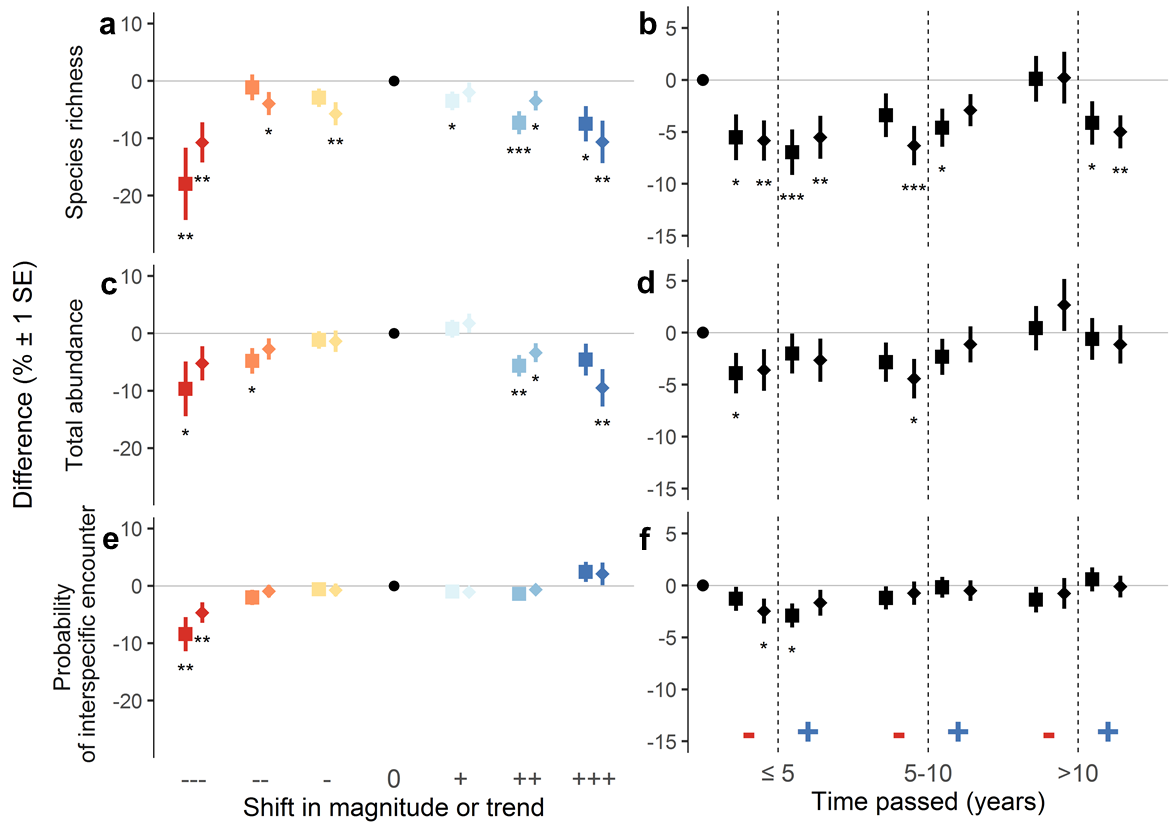
\includegraphics[width=1\textwidth]{chapter3/F02}
\caption{Local biodiversity impacts varied with attributes of abrupt land change. Differences in three measures of local biodiversity, (\textbf{a},\textbf{b}) species richness, (\textbf{c},\textbf{d}) total abundance, and (\textbf{e},\textbf{f}) the probability of interspecific encounter (PIE) at sites with an abrupt land change (squares, diamonds) relative to unchanged sites (0, black points). (\textbf{a},\textbf{c},\textbf{e}) Estimates are given separately for shifts in magnitude (squares; > 50\%, > 25\% to $\leq$ 50\%, and $\leq$ 25\% EVI loss [$---$ to $-$, coloured red to orange] or gain [$+++$ to $+$, blue to light blue], Appendix Figure \ref{SI03_02}\textbf{a}) or in EVI trend (diamonds; from $---$ to $+++$ for negative to positive trend differences, Appendix Figure \ref{SI03_02}\textbf{b}). (\textbf{b},\textbf{d},\textbf{f}) Impacts on biodiversity measures of time passed between an abrupt land change (gain/increase [$+$] or loss/decrease [$-$] in EVI shift in magnitude [squares] or trend [diamonds]) and sampling of biodiversity. Separate models were fitted for shifts in magnitude and in trend relative to unchanged sites (points). Error bars show fitted standard errors and asterisks statistical significance (* p < 0.05, ** p < 0.01, *** < 0.001) from the hierarchical models. For number of sites and studies for each bin and biodiversity measure see Appendix Figure \ref{SI03_04} and Table \ref{SIT03_01}}
\label{F03_02}
\end{figure}
% -------------------------------------------- %


\section{Results}
\label{C03_03}
Local biodiversity measures are lower at sites with an abrupt land change in the past. Sites at which an abrupt land change was observed contained on average 4.2\% fewer species (SE: 1.3\%, $\chi^2$ = 10.27, df = 3, p < 0.01), 2\% fewer individuals (SE: 1.3\%; $\chi^2$ = 72.9, df = 3, p < 0.001), and species assemblages were 1\% less even (SE: 0.6\%; $\chi^2$ = 42.79, df = 3, p < 0.001) compared to unchanged sites (Figure 2). Sites with larger abrupt shifts in magnitude and trend had fewer species and individuals than unchanged sites regardless of direction of abrupt land change (Figure \ref{F03_02}\textbf{a},\textbf{c}). Sites with > 50\% loss or gain in EVI had on average 18\% (SE: 6.4\%) or 9\% (SE: 3.2\%) fewer species, and 10\% (SE: 5\%) or 5\% (SE: 3\%) fewer individuals than unchanged sites (Figure \ref{F03_02}\textbf{a},\textbf{c}). Compared to unchanged sites, species assemblages were less even at sites with larger abrupt losses in EVI, but not at sites with larger gains in EVI (Figure \ref{F03_02}\textbf{e}). We found similar impacts of shifts in magnitude and trend on species richness ($\Delta$AIC = 3.22, Pearson’s r between impacts = 0.71), abundance ($\Delta$AIC = 2.64, r = 0.61), and evenness ($\Delta$AIC = 5.66, r = 0.98).

Biodiversity can recover after an abrupt land change depending on time passed. We hypothesize that with more time passed local biodiversity recovers to levels comparable to unchanged sites. In line with our expectation we found that sites with an abrupt land change up to five years before biodiversity sampling had on average 6.6\% fewer species (SE: 1.8\%), 3\% fewer individuals (SE: 1.8\%) and were 2\% less even (SE: 0.1\%) than unchanged sites (Figure \ref{F03_02}\textbf{b},\textbf{d},\textbf{f}). After more than 10 years had passed, biodiversity measures were comparable to unchanged sites (Figure \ref{F03_02}\textbf{b},\textbf{d},\textbf{f}), except for local species richness at sites with positive shifts in magnitude or trend (-4\%; Figure \ref{F03_02}\textbf{b}). Overall, we found similar impacts of shifts in magnitude and trend and varying time passed for species richness ($\Delta$AIC = 2.85, Pearson’s r between impacts r = 0.66), abundance ($\Delta$AIC = 2.46, r = 0.42), and evenness ($\Delta$AIC = 3.03, r = 0.65).

% ---------------- Figure 3 --------------------- %
\begin{figure}[ht]
\centering
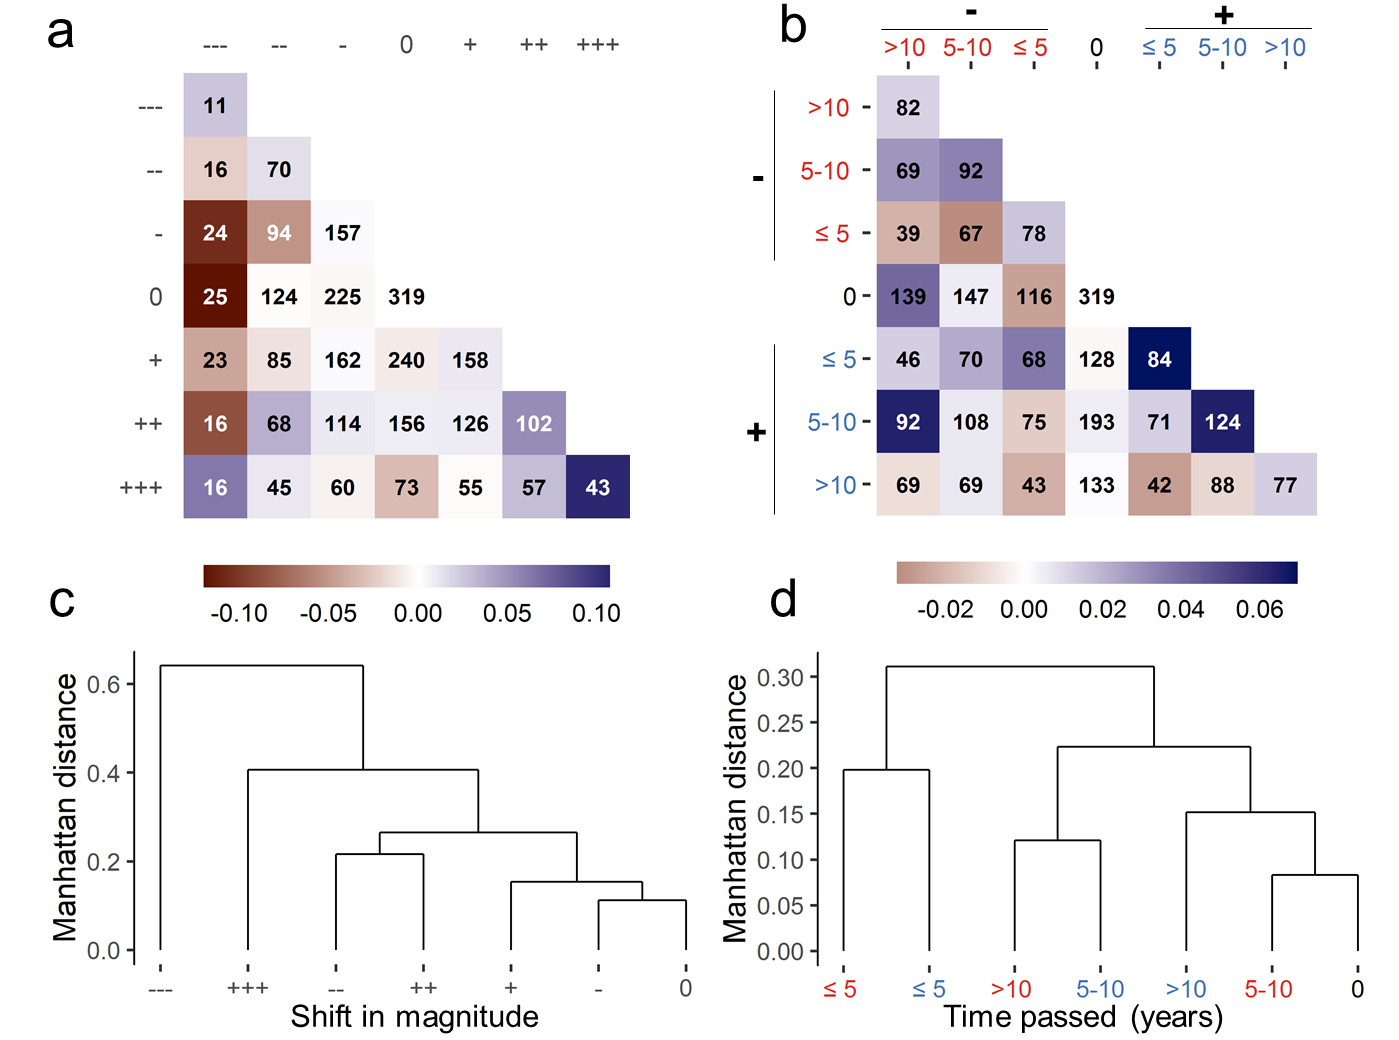
\includegraphics[width=1\textwidth]{chapter3/F03}
\caption{Reduced compositional similarity between sites without and with an abrupt land change. Mean similarity in species assemblage composition (S\o rensen similarity index) calculated between pairs of sites within the same study and land-use category without ($0$) and with an abrupt land change of (\textbf{a}, \textbf{c}) varying shifts in magnitude, or (\textbf{b}, \textbf{d}) loss or gain in EVI ($-$ and $+$) and time passed between abrupt land change and biodiversity sampling (axis labels as in Figure \ref{F03_02}). Colours indicate whether similarity of species assemblages was on average greater (purple) or smaller (brown) relative to unchanged sites. Numbers (in \textbf{a},\textbf{b}) indicate the total number of studies for which pairwise comparisons between sites could be made. All estimates are transformed relative to the compositional similarity between pairs of sites without a land change ($0 - 0$). (\textbf{c},\textbf{d}) Dendrograms show hierarchical clustering of all pairwise similarities based on the average Manhattan distance between pairs of sites; sites with more similar assemblage composition are in branches of closer proximity. }
\label{F03_03}
\end{figure}
% -------------------------------------------- %

Abrupt land change affects the composition of species assemblages. Species assemblages at sites with larger abrupt shifts in magnitude were less similar in composition to unchanged sites (Figure \ref{F03_03}\textbf{a}, \textbf{c}). Especially sites with a shift in magnitude of > 50\% EVI loss or gain were on average less similar (-0.12 / -0.03, respectively) in assemblage composition to unchanged sites (Figure \ref{F03_03}\textbf{a}). Furthermore, the composition of species assemblages was most dissimilar to unchanged sites if an abrupt land change occurred less than five years ago (Figure \ref{F03_03}\textbf{b},\textbf{d}). After more than five years had passed between an abrupt land change and biodiversity sampling, species assemblages were on average more similar in composition (0.04 / 0.001 for loss and gain in EVI, respectively) to unchanged sites (Figure \ref{F03_03}\textbf{b}). The composition of species assemblages was on average more similar among sites of comparable shifts in magnitude or with time passed (diagonals in Figure \ref{F03_03}\textbf{a},\textbf{b}) relative to unchanged sites. The impacts of abrupt shifts in magnitude were broadly comparable to shifts in trends although negative shifts in trend impacted assemblage composition more (Appendix Figure \ref{SI03_05}).

% ---------------- Figure 4 --------------------- %
\begin{figure}[!htb]
\centering
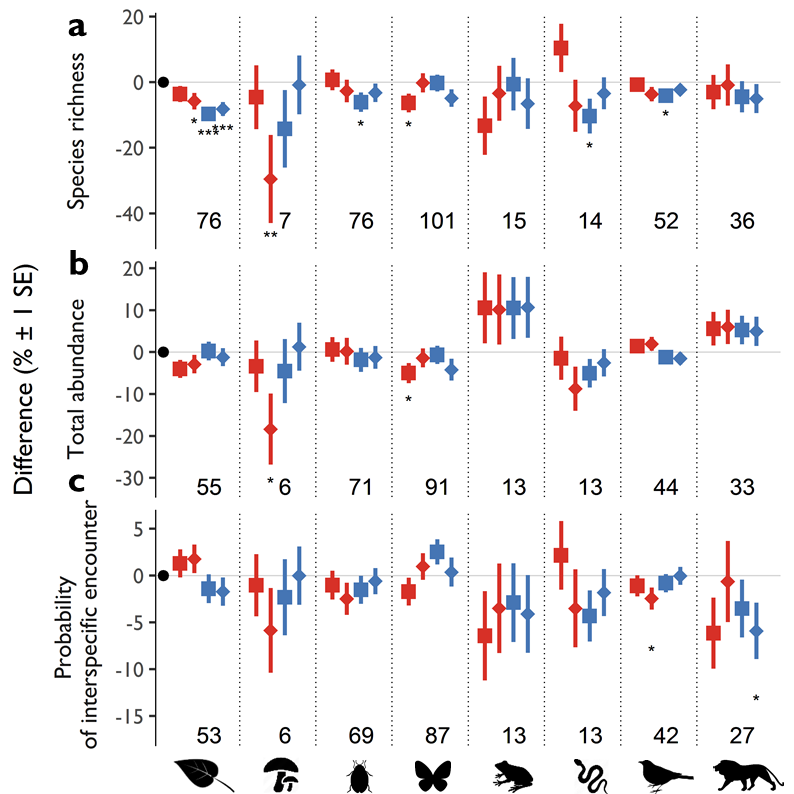
\includegraphics[width=1\textwidth]{chapter3/F04}
\caption{Abrupt land change affects taxonomic groups differently. Difference in (\textbf{a}) species richness, (\textbf{b}) total abundance, and (\textbf{c}) assemblage evenness for taxonomic groups (plants, fungi, ground dwelling invertebrates, flying invertebrates, amphibians, reptiles, birds, and mammals) between sites without and with an abrupt land change. Separate models were fitted for taxonomic groups comparing sites with shifts in magnitude (squares) and trend differences (diamonds) where colours indicate negative (red) and positive (blue) direction and sites without abrupt land change (black points, grey line). Error bars show standard errors and asterisks indicate statistical significance (* p < 0.05, ** p < 0.01, *** < 0.001). Numbers give the number of studies included per taxonomic group.}
\label{F03_04}
\end{figure}
% -------------------------------------------- %

Impacts of abrupt land changes in the past varies among taxonomic groups. Sites with a positive shift in magnitude had significantly fewer species of plant (9.7\%), bird (4.2\%), ground dwelling invertebrate (6.4\%), and reptile (10.4\%) compared to unchanged sites (Figure \ref{F03_04}\textbf{a}). Particularly sites with a negative shift in trend had significantly fewer species of plant (8.2\%, Figure \ref{F03_04}\textbf{a}) and fungi (29.6\%), and fewer individuals of fungi (17.8\%, Figure \ref{F03_04}\textbf{b}) compared to unchanged sites. The number of individuals and assemblage evenness was overall lower at sites with an abrupt land change compared to unchanged sites, although amphibian and mammal abundance as well as evenness of flying insects was higher at sites with an abrupt land change (Figure \ref{F03_04}\textbf{b},\textbf{c}). For most taxonomic groups, except fungi and reptiles, there was little difference between the impacts of shifts in magnitude or trend on biodiversity measures (Figure \ref{F03_04}).

\section{Discussion}
\label{C03_04}
We found species assemblages to be negatively impacted by past abrupt land change. Larger changes on land caused greater reductions in local biodiversity (Figure \ref{F03_02}\textbf{a}-\textbf{c}) regardless of whether shifts in magnitude or trend of photosynthetic activity (EVI) were positive or negative, suggesting general impacts of past abrupt land change on biodiversity \citep{Dornelas2010,Hautier2015} likely caused by biotic lag effects \citep{Hylander2013,Ogle2015,Jung2018}. Abrupt land changes with large (>50\%) losses or gains in EVI have caused immediate and time-delayed local extinctions \citep{Krauss2010,Halley2016,Wood2017}, and reduced the abundance and dominance of persisting species (Figure \ref{F03_02}\textbf{b}-\textbf{c}), which may ultimately affect ecosystem functioning \citep{Hautier2015,Isbell2015}. Previous studies predicted assemblage evenness to increase with change magnitude \citep{Svensson2012}, however our results demonstrate this to be only the case for positive changes in photosynthetic activity (\ie a gain or positive trend shift in EVI). Abrupt land changes can alter the composition of species assemblages with early colonizing and non-native species often outperforming or replacing many persisting species \citep{Fraterrigo2006,Turner2010,Jauni2015}, which could explain the observed impacts on species assemblage evenness (Figure \ref{F03_02}\textbf{c}) and compositional similarity (Figure \ref{F03_03}).

The recovery from abrupt land change is of important concern for biodiversity conservation \citep{Chazdon2003}. We found biodiversity measures to be lower (Figure \ref{F03_02}\textbf{b},\textbf{d},\textbf{f}) and the composition of species assemblages altered more compared to unchanged sites (Figure \ref{F03_03}\textbf{b},\textbf{d}) if an abrupt land change occurred relatively recently (< 5 years). An explanation could be that some, disturbance sensitive, species are immediately lost from local assemblages because of an abrupt land change \citep{Devictor2008,Supp2014}. However local biodiversity can recover from an abrupt land change with biodiversity measures being comparable to unchanged sites after >10 years \citep{Martin2013,Moreno-Mateos2017}, although local species richness did not recover at sites where EVI had increased (Figure \ref{F03_02}\textbf{b}). Land changes causing an abrupt positive shift could be related to increase or sudden cessation of anthropogenic use intensity \citep{Eastman2013,Muller2014}, which may have caused further local species loss \citep{Tilman1994,Balmford1996,Hylander2013}. Nevertheless, the time passed since an abrupt land change occurred can be a poor predictor of biodiversity recovery as land trajectories are often highly unpredictable \citep{Norden2015} or include multiple land changes \citep{Watson2014}. We suggest future analyses to consider how additional attributes, such as trajectories or frequency of land change \citep{Watson2014}, influence local biodiversity recovery. 

A number of other factors mediate the response of local biodiversity to land change \citep{Arroyo-Rodriguez2015}.  Previous studies demonstrated local biodiversity to recover quicker from an abrupt land change with a greater availability of undisturbed land in the wider landscape \citep{Turner1989,Chase2003,Shackelford2017}. In addition, site-specific factors and a long history of human modification can mediate the impact of abrupt land change on local biodiversity \citep{Ellis2015a,Jung2016}, especially since the majority of sites in the PREDICTS database are in regions that have long been subjected to human influence \citep{Newbold2016a,Hudson2016}. It is likely that some species \textendash\ those particularly sensitive to land changes \textendash\ have been lost from local assemblages long before the availability of Landsat data (< 1982) and we expect the found impacts of abrupt land change on biodiversity to be conservative \citep{Mihoub2017}. Land changes can also be characterized by attributes not considered in this study, such as frequency and trajectory \citep{Watson2014}, which have been shown to influence local biodiversity \citep{Tiemann2015,Wood2017} and for many types of land change events \textendash\ such as harvests, grazing or fallow period cycles \citep{Kleyer2007,Ray2013} \textendash\ are often similar in shifts of magnitude and trend. Future studies should evaluate the influence of differing land trajectories and frequencies of land change on local biodiversity.

What drives abrupt land change events? Abrupt land change, identified by shifts in magnitude and/or trend of photosynthetic activity, can be caused by anthropogenic deforestation \citep{DeVries2015b}, land intensification \citep{Fensholt2012,Muller2014}, or degradation \citep{Tian2015,Aguiar2017}. In this study we did not separate between natural and anthropogenic drivers of abrupt land change and changes in photosynthetic activity can also be caused by rainfall-driven anomalies \citep{Papagiannopoulou2017} or changing nitrogen deposition and CO2 fertilization \citep{Zhu2016}. Most PREDICTS sites are modified by humans \citep{Newbold2016a,Hudson2016} and it is therefore likely that most detected land changes were caused by humans. Future studies should attempt to distinguish and disentangle the impacts of natural and anthropogenic abrupt land changes \citep{Curtis2018}. 

Detecting and quantifying abrupt land changes is challenging. Here we focussed on detecting abrupt land change as shifts in magnitude or trend \citep{Verbesselt2010a}, but not all land change is abrupt \citep{Vogelmann2012a} or \textendash\ such as understory thinning and selective logging \textendash\ can be detected in time series of remotely-sensed photosynthetic activity \citep{Asner2005,Peres2006}. Similar to previous studies we assessed only the impact of the single largest shift in magnitude or trend \citep{dejong2013,Song2018}, while different sequences of land change may also affect local biodiversity \citep{Watson2014}. Future studies quantifying abrupt land change globally could benefit from better access to, or fusion of, available satellite data to reach higher temporal and spectral resolution \citep{Reiche2015,Wulder2015}.

In conclusion, we demonstrate that compared to unchanged sites local biodiversity is considerably reduced because of abrupt land changes in the past, potentially affecting the stability and functioning of ecosystems \citep{Hautier2015}. Ignoring delayed biodiversity responses to abrupt land changes means that contemporary biodiversity changes, loss and recovery, are underestimated \citep{Kuussaari2009,Essl2015}. Conservation practitioners need to consider the impacts of biotic lag effects to ensure global and regional assessments (\eg those by the Intergovernmental Science-Policy Platform on Biodiversity and Ecosystem Services [IPBES]) fully capture biodiversity change \citep{Essl2015}. Remote sensing can assist in quantifying attributes of abrupt land change over large spatial and temporal scales. Our analytical framework can be expanded to assess spatial prioritization of habitat restoration plans or to support scenario-based modelling \citep{Ewers2009} to predict the impacts of abrupt land change on local biodiversity.

\section{Data and code availability}
\label{C03_05}
The PREDICTS biodiversity data are publicly available in the Natural History Museum Data Portal (\doi{10.5519/0066354}, \cite{Hudson2016}). All remote sensing data are accessible via Google Earth Engine (\href{earthengine.google.com/}{earthengine.google.com/}) \citep{Gorelick2017} and pre-processed time series will be deposited on GitHub (\href{https://github.com/Martin-Jung/PastDisturbance}{https://github.com/Martin-Jung/PastDisturbance}) on publication.Data and code to reproduce the results will be made available in a GitHub repository (\href{https://github.com/Martin-Jung/PastDisturbance}{https://github.com/Martin-Jung/PastDisturbance}) on publication.

\clearpage
%\bibliography{content/04Chapter}

%\appendix
%\begingroup
%  % SI - Figure 1 Missing data
\begin{figure}[h]
\centering
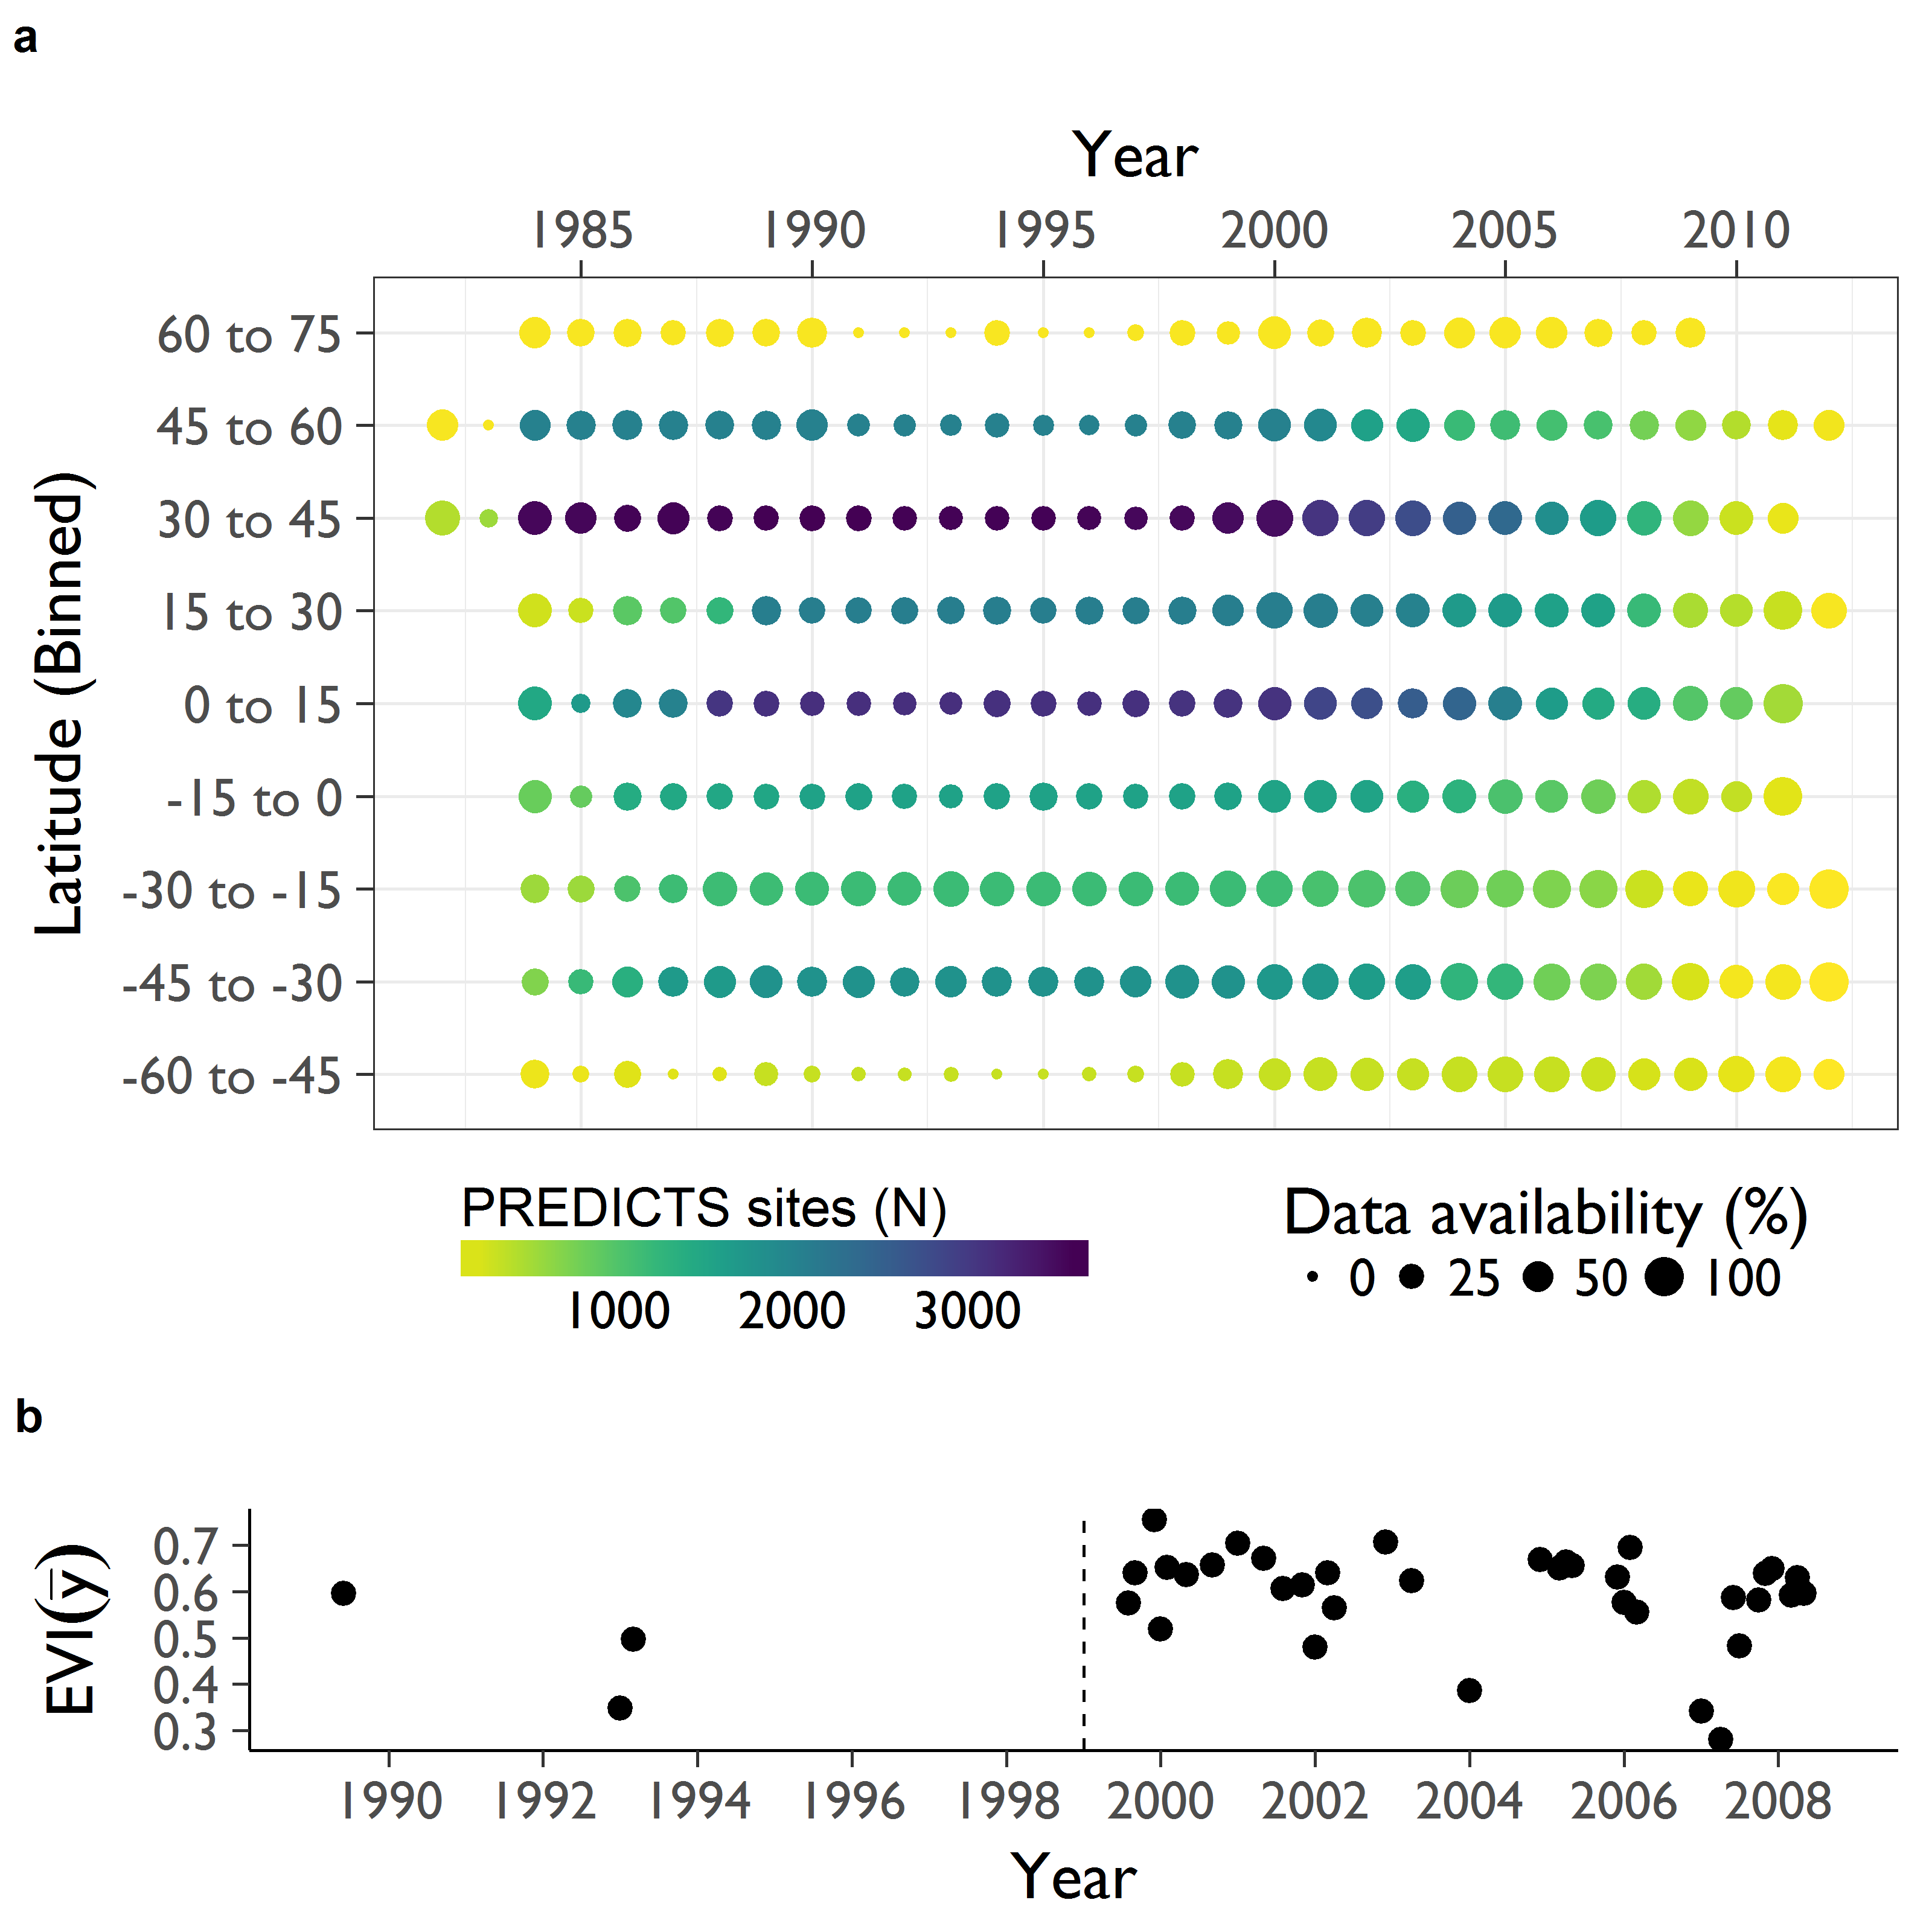
\includegraphics[width=1\textwidth]{chapter3/SI01}
\caption{ Average temporal distribution of Landsat data and an example times series of Landsat data. (\textbf{a}) Distribution of available Enhanced Vegetation Index (EVI) data in years covered by the Landsat missions. Points show the average monthly EVI data availability per year (0 to 12 months of data) across time series and PREDICTS sites grouped by 15\textdegree latitude bins. The size of points indicates the mean data availability (0 to 100\% with 100\% having 12 months of available data in a given year), while the colour shows the number of PREDICTS sites contributing to the mean (as PREDICTS sites were sampled in varying years). (\textbf{b}) Example time series for one PREDICTS site with a high proportion of missing data before 1999. In all analyses such time series were truncated to the period from 1999 onwards (indicated by the dashed line).}
\label{SI03_01}
\end{figure}

% SI - Figure 2 Binning
\begin{figure}[h]
\centering
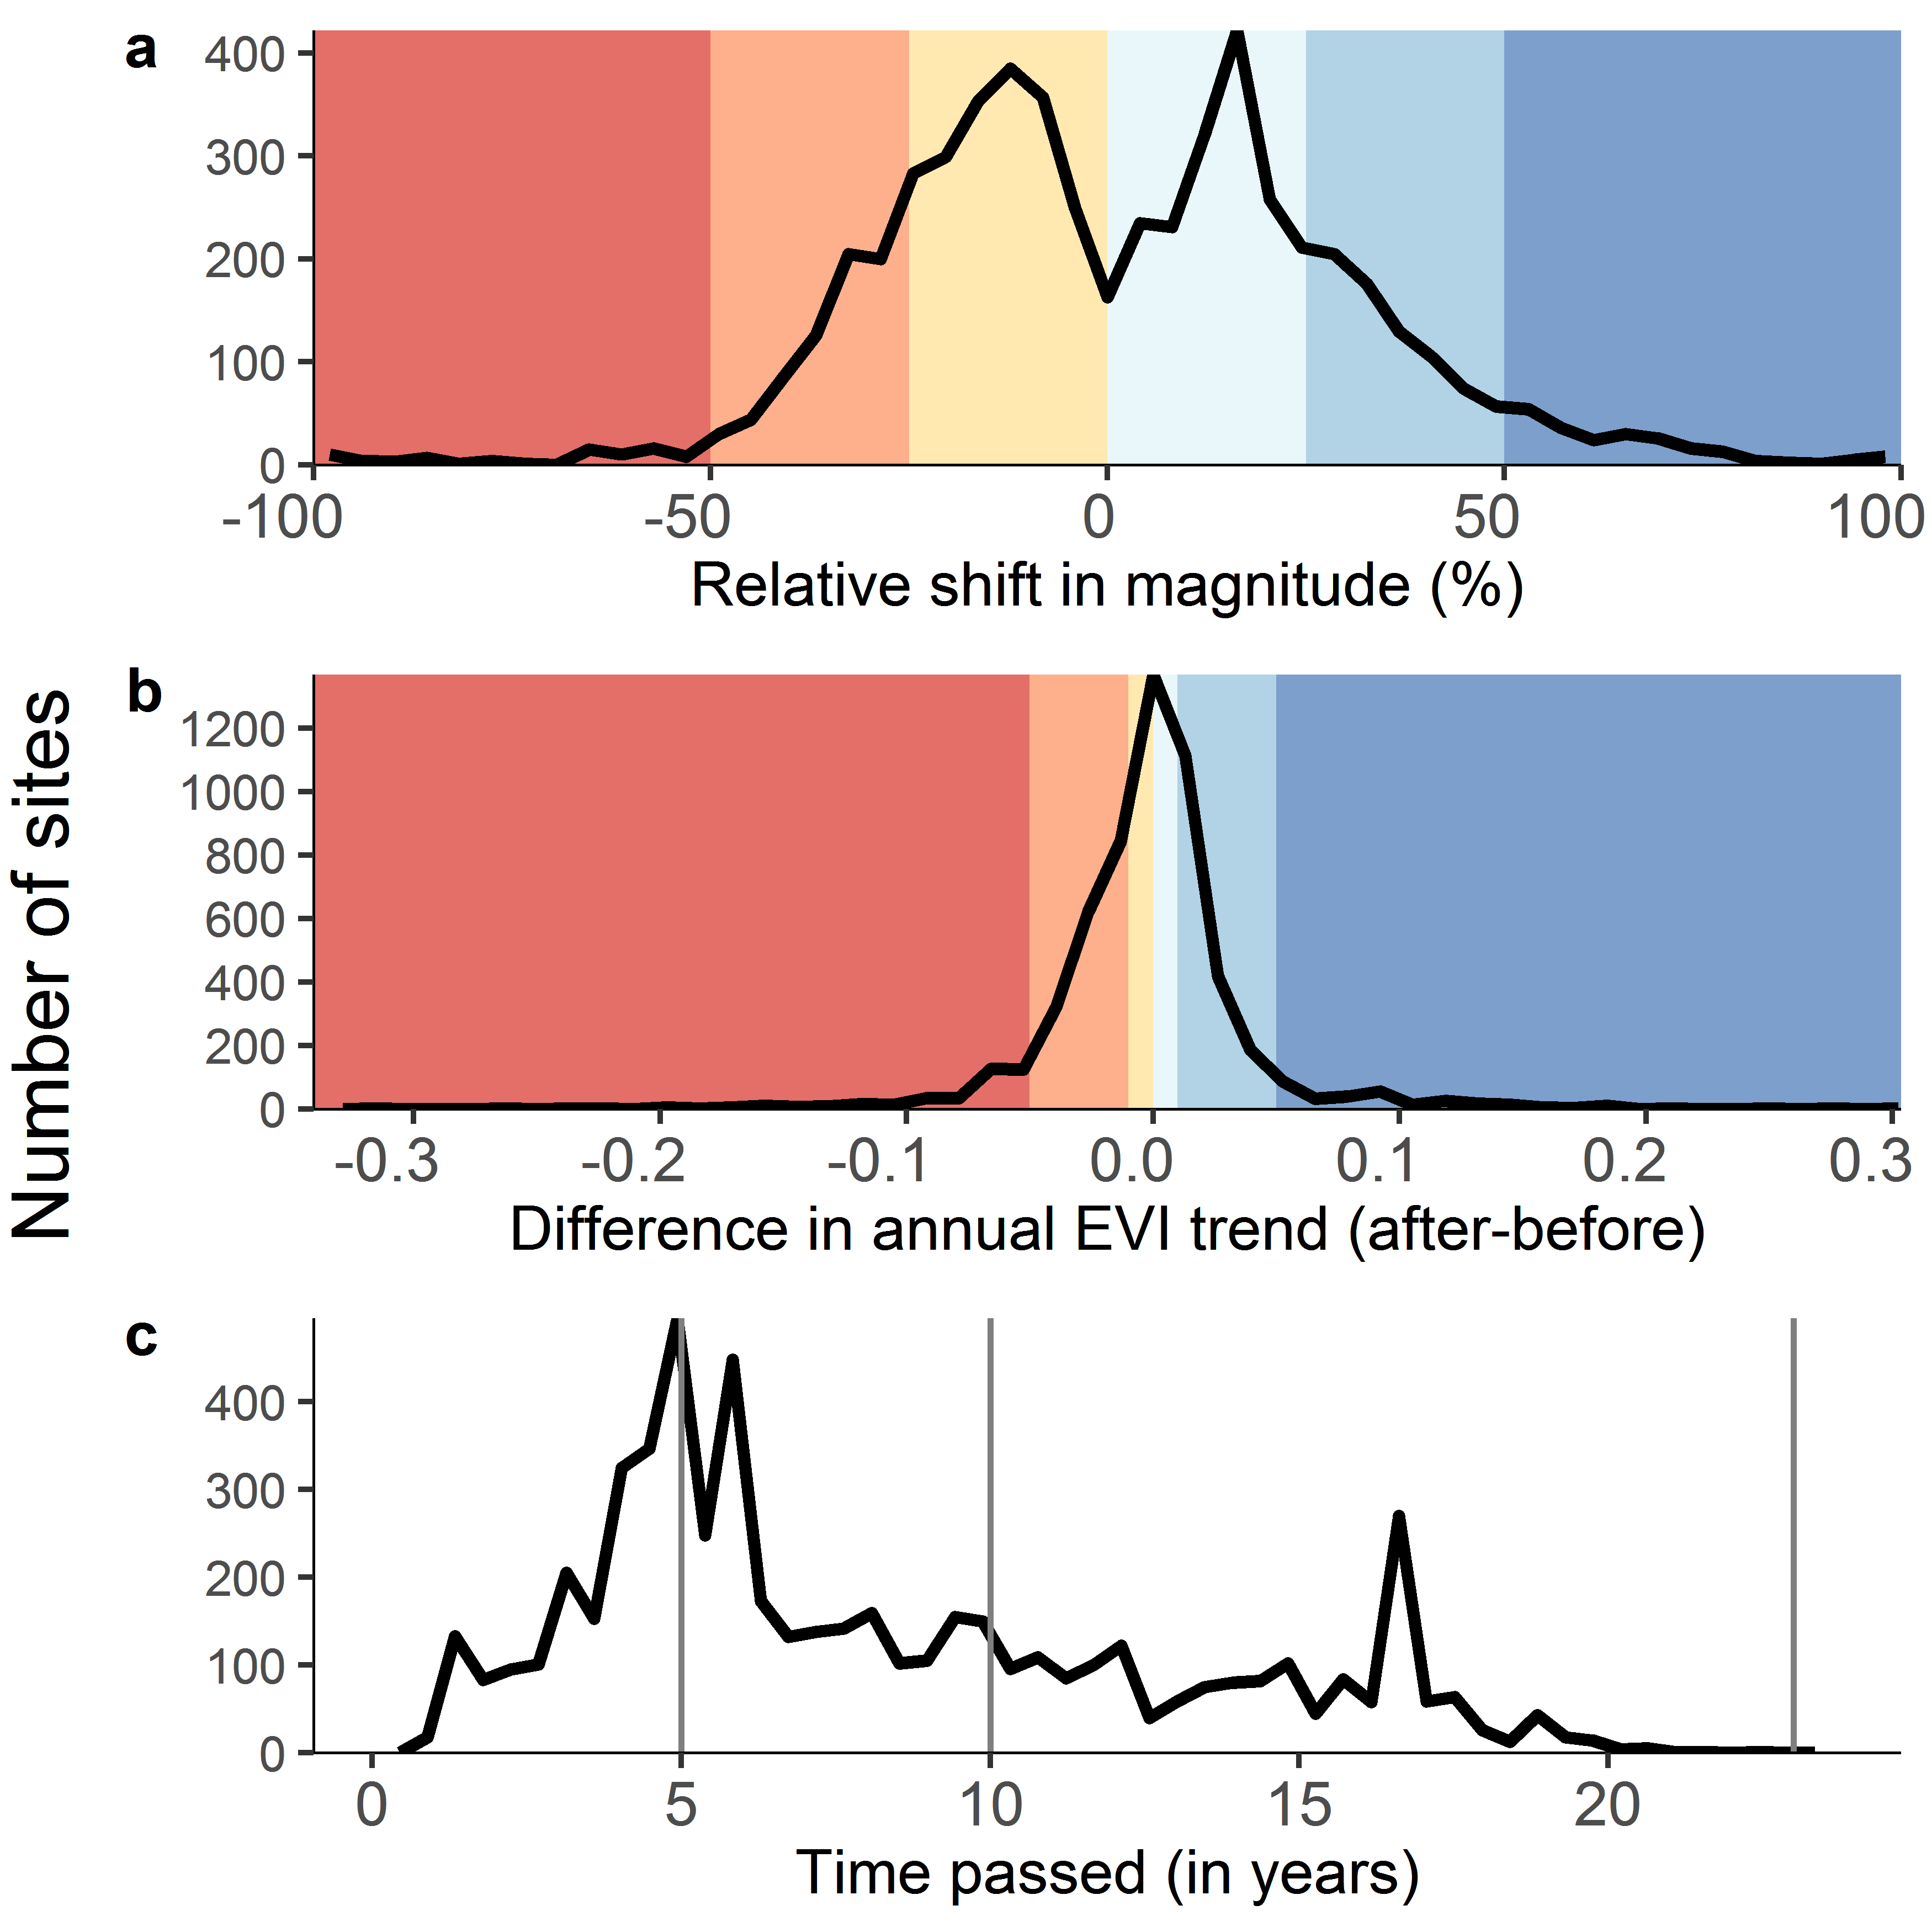
\includegraphics[width=1\textwidth]{chapter3/SI02}
\caption{ Number of sites with abrupt land change per attribute. Number of sites (black line) per attribute of abrupt land change with (\textbf{a}) the relative shift in magnitude, (\textbf{b}) the shift in trend as difference in annual EVI trend, and (\textbf{c}) the time passed between abrupt land change and biodiversity sampling. Background colours in (\textbf{a}) and (\textbf{b}) indicate the binning into six groups for shifts in magnitude (> 50\%, > 25\% to $\leq$ 50\%, and $\leq$ 25\% EVI loss [$---$ to $-$] or gain [$+++$ to $+$]), and in trend (0.01, 0.05, and > 0.05 annual negative [$---$ to $-$] to positive [$+++$ to $+$] EVI trend differences). Gray lines in (\textbf{c}) delineate bins of time passed ($\leq$ 5 years, > 5 and $\leq$ 10 years, and >10 years). Colours as in Figure \ref{F03_02}.}
\label{SI03_02}
\end{figure}

% SI Table 1------ %
% From here https://www.tablesgenerator.com/
\begin{table}[]
\centering
\caption{Number of PREDICTS sites and studies with an abrupt land change. Shown as either a change in magnitude (columns) and/or change in trend (trend). Symbols as in Figure \ref{F03_02}. }
\label{SIT03_01}
\begin{tabular}{@{}lllllllllll@{}}
                                          &                                           & \multicolumn{7}{c}{\textbf{Shift in magnitude}}                                                                                                                                                                    &                               &                             \\
                                          &                                           & \textbf{- - -}             & \textbf{- -}                & \textbf{-}                   & \textbf{0}                    & \textbf{+}                   & \textbf{+ +}                & \textbf{+ + +}              & \textbf{Total sites}          & \textbf{Studies}            \\ \cmidrule(l){3-11} 
                                          & \multicolumn{1}{l|}{- - -}                & 2                          & 8                           & 192                          & NA                            & 73                           & 26                          & 22                          & \cellcolor[HTML]{EFEFEF}323   & \cellcolor[HTML]{C0C0C0}57  \\
                                          & \multicolumn{1}{l|}{- -}                  & 7                          & 281                         & 642                          & NA                            & 497                          & 158                         & 53                          & \cellcolor[HTML]{EFEFEF}1638  & \cellcolor[HTML]{C0C0C0}175 \\
                                          & \multicolumn{1}{l|}{-}                    & 7                          & 88                          & 256                          & NA                            & 231                          & 154                         & 53                          & \cellcolor[HTML]{EFEFEF}789   & \cellcolor[HTML]{C0C0C0}184 \\
                                          & \multicolumn{1}{l|}{0}                    & NA                         & NA                          & NA                           & 10102                         & NA                           & NA                          & NA                          & \cellcolor[HTML]{EFEFEF}10102 & \cellcolor[HTML]{C0C0C0}358 \\
                                          & \multicolumn{1}{l|}{+}                    & 9                          & 102                         & 399                          & NA                            & 410                          & 205                         & 49                          & \cellcolor[HTML]{EFEFEF}1174  & \cellcolor[HTML]{C0C0C0}237 \\
                                          & \multicolumn{1}{l|}{\textbf{+ +}}         & 47                         & 172                         & 342                          & NA                            & 465                          & 254                         & 86                          & \cellcolor[HTML]{EFEFEF}1366  & \cellcolor[HTML]{C0C0C0}224 \\
\multirow{-7}{*}{\textbf{\rotatebox{90}{Shift in trend}}} & \multicolumn{1}{l|}{\textbf{+ + +}}       & 12                         & 137                         & 47                           & NA                            & 34                           & 12                          & 31                          & \cellcolor[HTML]{EFEFEF}273   & \cellcolor[HTML]{C0C0C0}56  \\
                                          & \multicolumn{1}{l|}{\textbf{Total sites}} & \cellcolor[HTML]{EFEFEF}84 & \cellcolor[HTML]{EFEFEF}788 & \cellcolor[HTML]{EFEFEF}1878 & \cellcolor[HTML]{EFEFEF}10102 & \cellcolor[HTML]{EFEFEF}1710 & \cellcolor[HTML]{EFEFEF}809 & \cellcolor[HTML]{EFEFEF}294 &                               &                             \\
                                          & \multicolumn{1}{c|}{\textbf{Studies}}     & \cellcolor[HTML]{C0C0C0}34 & \cellcolor[HTML]{C0C0C0}135 & \cellcolor[HTML]{C0C0C0}246  & \cellcolor[HTML]{C0C0C0}358   & \cellcolor[HTML]{C0C0C0}263  & \cellcolor[HTML]{C0C0C0}171 & \cellcolor[HTML]{C0C0C0}83  &                               &                            
\end{tabular}
\end{table}
% ------ %

% SI - Figure 3 Cross-correlations
\begin{figure}[h]
\centering
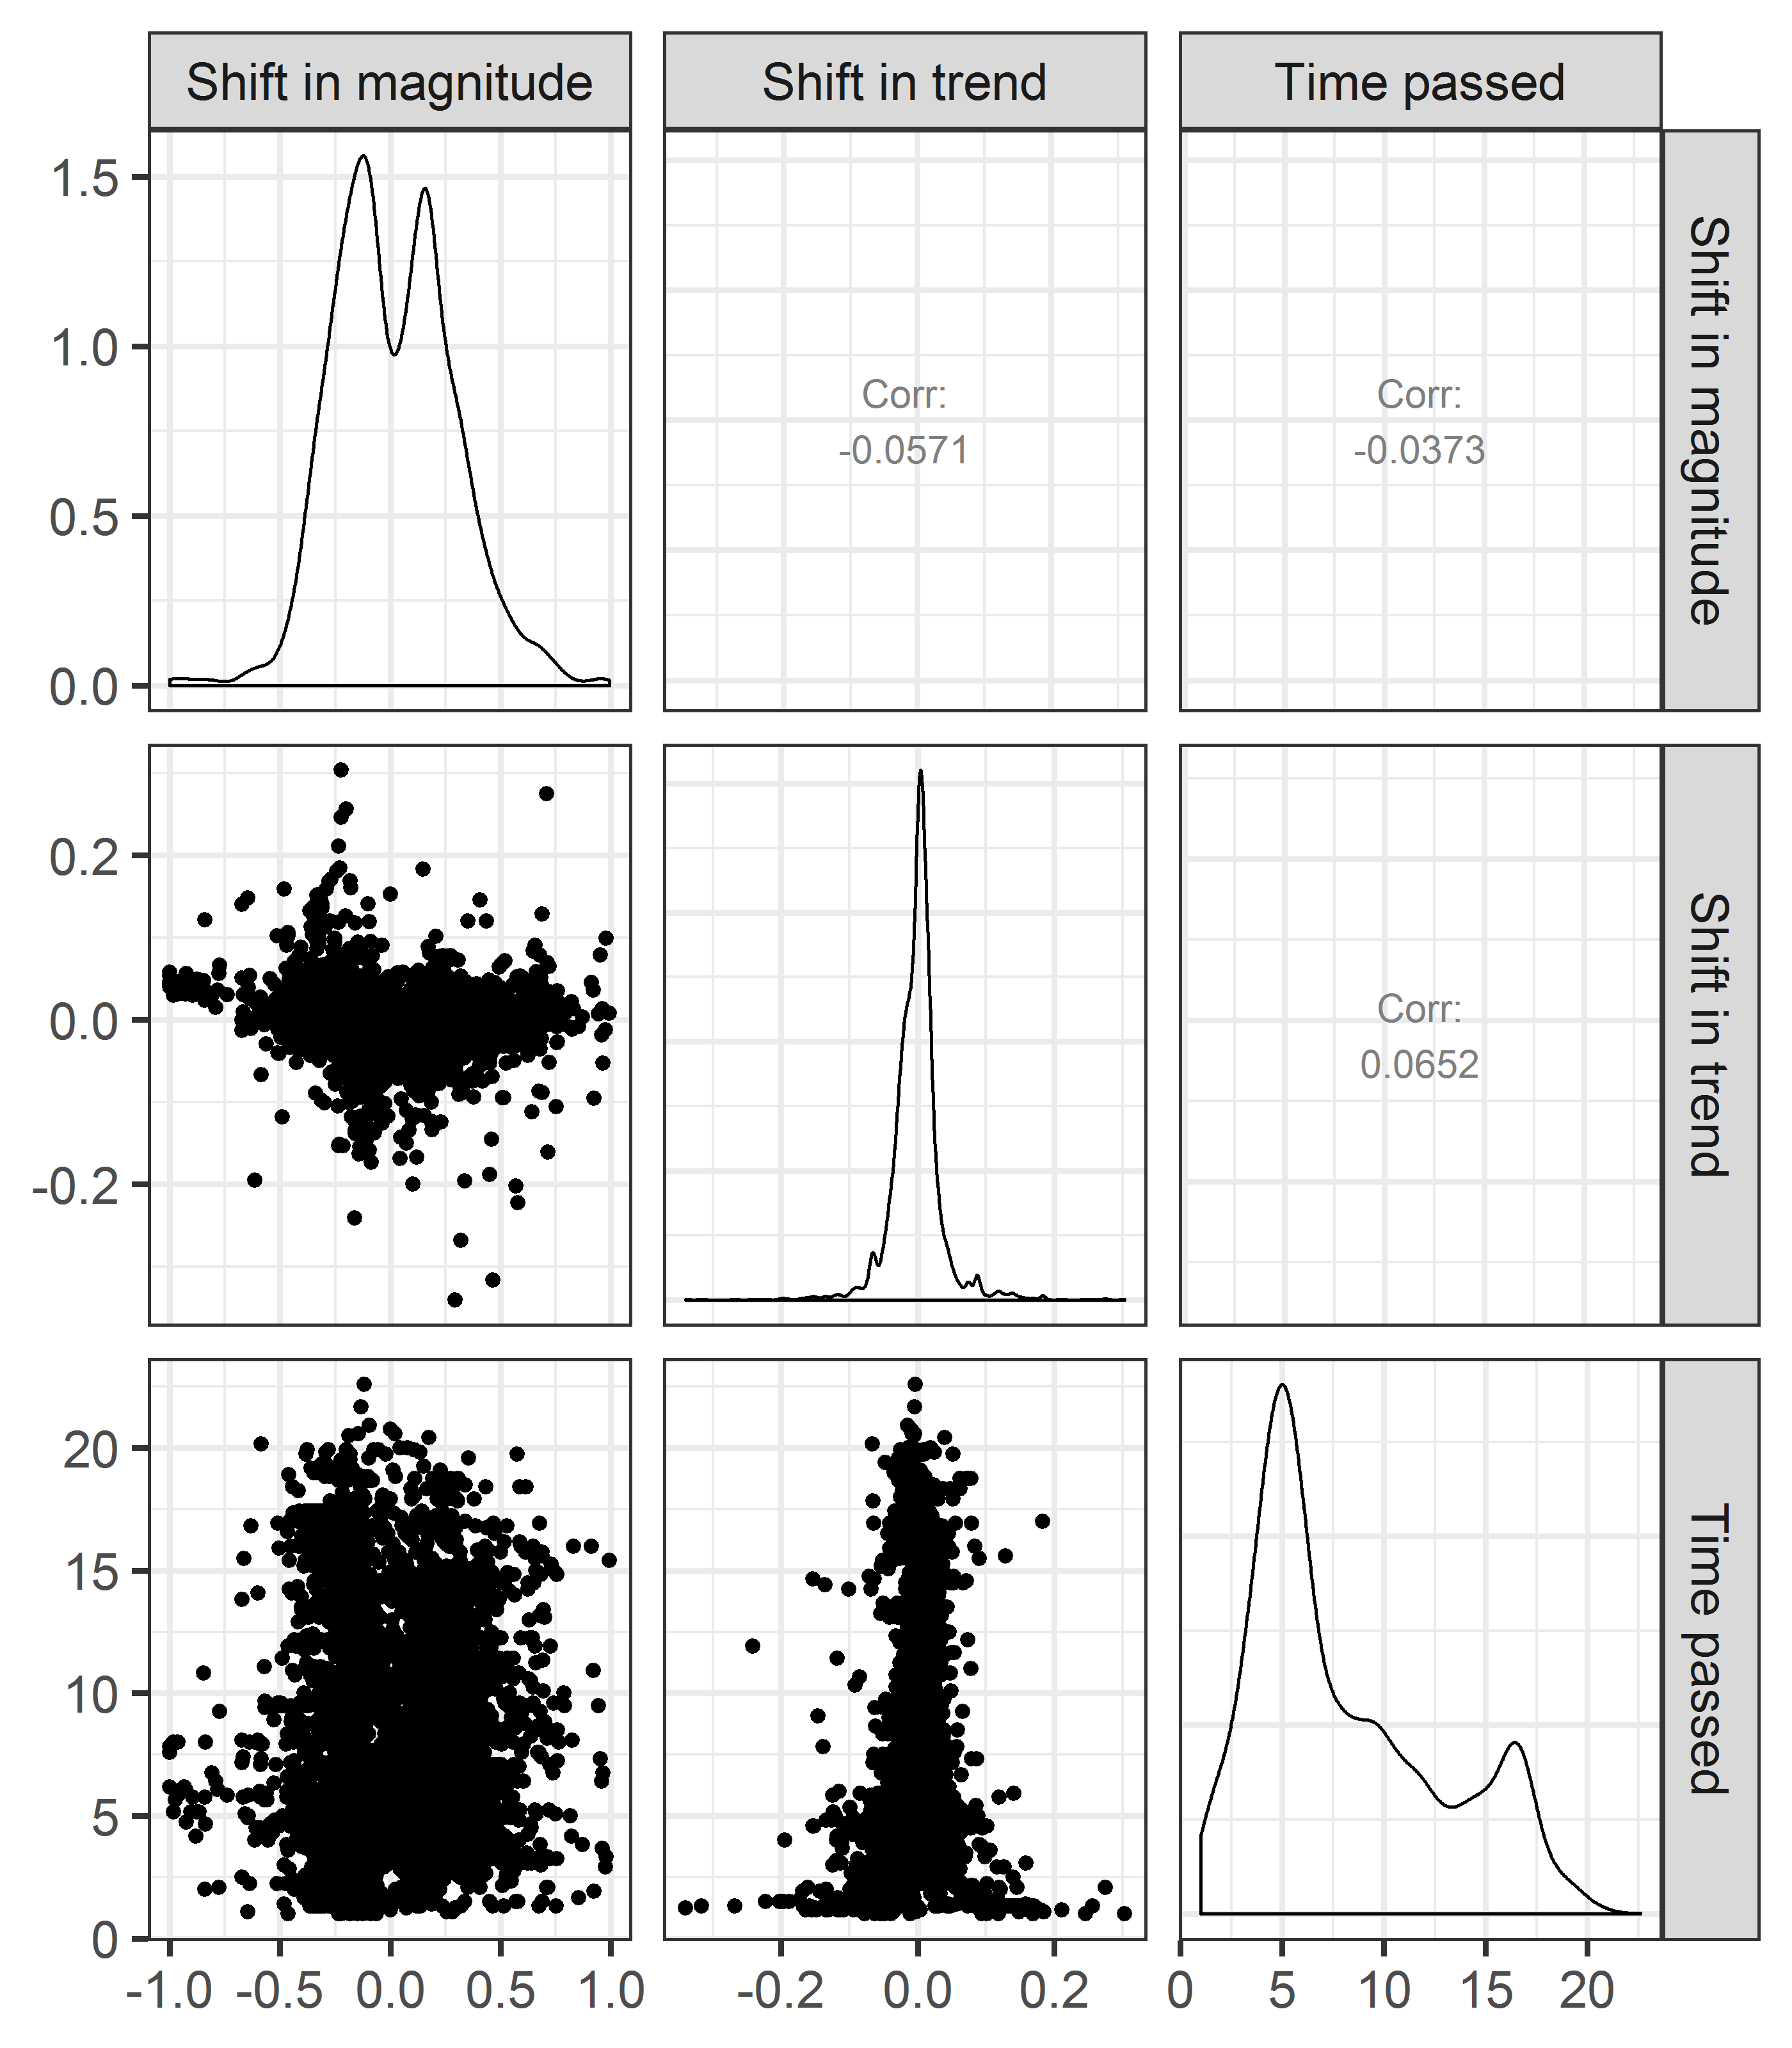
\includegraphics[width=1\textwidth]{chapter3/SI03}
\caption{ Correlations between attributes of abrupt land change. Showing shifts in magnitude, trend and time passed (see Methods). The lower facets show a point density plot, the upper facets the Pearson correlation coefficient between pairs of attributes and the diagonal a density plot.}
\label{SI03_03}
\end{figure}

%\endgroup
 %Abrupt land change
  %\chapter{Incorporating land-cover changes between 1992 and 2015 into biodiversity projections }
%\addcontentsline{toc}{chapter}{Chapter 4}
%\markboth{}{Incorporating land-cover changes between 1992 and 2015 into biodiversity projections }
\label{C04}

Changes in global land cover are important factors that determine past and present biodiversity patterns. It has been proposed that attributes of land-cover change, such as the time passed or the sequence in land cover \textendash\ \ie from forest to agriculture \textendash\ likely affect local biodiversity differently. Local biodiversity might continue to be affected by past land-cover change depending these attributes, which need to be considered to assess biodiversity change, especially in global and national biodiversity projections. Yet, the impacts of attributes of past land-cover change on local biodiversity have not been fully determined globally and most existing biodiversity projections remain largely uninformed of past land-cover change. Here, we combine time series of annual land cover from the period 1992 to 2015 with data of local biodiversity globally. Using hierarchical models comparing sites with and without a land-cover change in the past, we ask whether biodiversity differences vary with the time passed or the sequence after a land-cover change occurred and how this affects global and national biodiversity projections. Overall, we found local biodiversity to be consistently lower in sites with a past land-cover change. However, with increasing time passed after land-cover change local biodiversity recovered to levels comparable to unchanged sites. Furthermore, depending on the land-cover sequence, we observed either increases or decreases in local biodiversity and we demonstrated how a consideration of past land-cover change affects global and national biodiversity projections, especially so in tropical and economically developing countries. Our findings have implications for global biodiversity models given that most past and future projections of biodiversity ignore lasting influences of past land-cover changes. 

\section{Introduction}
\label{C04_01}

The terrestrial surface of the Earth is shaped by natural and anthropogenic processes \citep{Foley2005}. The outcomes of these processes alter soil, plant and human structures, which collectively define terrestrial land cover \citep{DiGregorio2000,Lambin2006}. Land cover \textendash\ quantified as either continuous or categorical estimate of the Earth land surface conditions \textendash\ is commonly derived from remotely-sensed spectral measurements with many studies having mapped the distribution of land-cover categories globally \citep{DeFries1994,Hansen2000,Tuanmu2014,Grekousis2015}. Knowledge of land-cover change is important to help understand biodiversity change and create future projections and scenarios \citep{Harfoot2014,Titeux2016,Newbold2016,Kehoe2017a}. Yet, with exception of vegetation \citep{Hansen2013,Song2018}
or water-covered areas \citep{Pekel2016}, few temporally consistent estimates of global land-cover change exist.

Quantifying change in remotely-sensed land cover is challenging. For continuous representations of land cover, remotely-sensed changes are commonly detected by exploiting differences in timing, amplitude and direction of remotely-sensed spectral measurements \citep{Coppin2004,Lhermitte2011,Zhu2017}. There have been initial attempts to incorporate land-cover changes detected from these differences into categorical land-cover maps \citep{Zhu2014,Hermosilla2018}, but the majority of land-cover maps remain uninformed of preceding land cover. Quantifying temporal change in categorical representations of land cover has been problematic because of inconsistencies in thematic resolution that lead to unrealistic estimates of land-cover change \citep{VERBURG2011,Cardille2016,Abercrombie2016}. A new generation of temporally consistent time series of land cover \citep{ESA2017,Hermosilla2018,Nowosad2018,Sulla-Menashe2019} are beginning to emerge that allow the investigation of land-cover change globally and its impacts on biodiversity.

Biodiversity is impacted by past and present differences in land cover \citep{Newbold2015,Newbold2016,Jung2018}. Local species richness has been estimated to be up to 31\% lower globally in the most anthropogenically modified land compared to “primary vegetation” sites \citep{Newbold2015}. However most previous global studies have considered only differences in land use and/or land cover at the time of biodiversity sampling \citep{Gibson2011,Murphy2014,Newbold2015}, thus ignoring lasting influences of past changes in land cover. There is evidence that the occurrence and abundance of species is not only determined by differences in present but also past land cover \citep[, Chapter \ref{C03}] through so called ‘biotic lag’ effects, such as ecological memory effects \citep{Ogle2015} or extinction debts \citep{Kuussaari2009}. The impact of past land-cover change on biodiversity likely depends on certain attributes such as magnitude and time passed since land-cover change \citep[Chapter \ref{C03}, ][]{Martin2013,Watson2014,Fu2017} or the sequences of land-cover \citep{Watson2014,Nowosad2018}. 

Land-cover change causes varying sequences of land cover \citep{Nowosad2018}, which often have differing impacts on local biodiversity \citep{Foster2003}. \cite{Bremer2010} reported an average loss of species richness globally for land changing from grass- or shrubland to forest cover, but not for land changing from secondary vegetation to forest cover. Meanwhile, biodiversity in secondary vegetation has been shown to recover more quickly if land was previously covered by grassland rather than agriculture \citep{Dyer2010}, although among taxonomic groups, especially plant diversity, abundance and growth have been shown to be influenced by lasting influences of an agricultural past \citep{Chazdon2003,Fraterrigo2006,DeFrenne2010,Perring2018}. Other studies have highlighted the lasting effect that changes in forest \citep{Gonzalez2016} or wetland cover \citep{Halstead2014} might have on biodiversity. While these studies suggest that land-cover sequences need to be considered for explaining differences in local biodiversity, little is known about the influence of land-cover sequences across taxonomic groups and at global and national scales, which could affect projections of biodiversity.

To guide decision making, projections of global and national biodiversity change are often useful to inform policy \citep{Pereira2010,Visconti2014}. Biodiversity projections can be used to create scenarios of biodiversity change in response to pressures such as land change \citep{Newbold2015,Newbold2016,Titeux2016}, which can inform science-policy platforms \citep{Harfoot2014,Visconti2014,Purvis2018} like as the Intergovernmental Platform on Biodiversity and Ecosystem Services (IPBES). However most existing biodiversity projections ignore lasting effects of past land-cover change. This is especially problematic for tropical, developing nations, where much land has been converted from forest to agriculture or pasture covered land in recent decades \citep{Curtis2018} and that are recognized as global biodiversity hotspots \citep{Brooks2002,Laurance2014}. Under a business-as-usual scenario of future biodiversity change, especially less economically developed countries will suffer the greatest losses in local biodiversity \citep{Newbold2015,Visconti2014}, however these projections might \textendash\ depending on attributes of land-cover change \textendash\ over- or underestimate impacts on biodiversity.

The overall aim of this study is to investigate (\textit{i}) how local biodiversity is impacted by a land-cover change in the past as derived from a global remotely-sensed land cover product, (\textit{ii}) if impacts on local biodiversity differ with attributes of land-cover change such as differing sequences of land cover or time passed \citep{Watson2014}, and (\textit{iii}) how particularly differing sequences of land cover affect global and national biodiversity projections. Overall, this study adds to our knowledge of how attributes of land-cover change affect local biodiversity and demonstrates how these attributes can be incorporated into global and national biodiversity projections.   

\section{Methods}
\label{C04_02}
\subsection{Species assemblage data}
\label{C04_0201}

The local biodiversity data were derived from a snapshot (obtained Feb 2016) of the Projecting Responses of Ecological Diversity In Changing Terrestrial Systems (PREDICTS) database which collated data on species’ presence and abundance at sampled ‘sites’ from published ‘studies’ \citep{Hudson2016}. Each PREDICTS site has associated spatial coordinates \textendash\ usually obtained from the text or author of a published study \textendash\ and a record of when and how long biodiversity sampling took place. Species assemblages in the PREDICTS database were sampled at various sampling extents (maximum linear extent, MLE) which are defined by methodology and taxonomic group \citep{Hudson2014}. To link local biodiversity with remotely-sensed land cover data (see \ref{C04_0202}), we used the spatial coordinates of all sites provided by the PREDICTS database as for the majority of sites the MLE is fully contained (median MLE = $40 \pm 56.49$ MAD) within the used grid cell size (\textasciitilde 300m, see methods \ref{C04_0202}).   

Similar to previous analyses using the same data (\eg Chapter \ref{C02} in this thesis), we calculated several biodiversity measures including the total number of species, individuals and the species assemblage evenness at the site level. We calculated local species richness and \textendash\ where data on species abundance was available \textendash\ the total abundance for each PREDICTS site. For those studies in PREDICTS with differing sampling effort among sites we corrected estimates of total abundance by assuming that total abundance increases linearly with sampling effort \citep{Newbold2014b,Newbold2015}. As a measure of assemblage evenness, we calculated the probability of an interspecific encounter (PIE), which quantifies the probability of two individuals randomly chosen from an assemblage representing different species \citep{Hurlbert1971}. 

\subsection{Annual land cover data}
\label{C04_0202}

We used estimates of land cover (LC) from a global dataset produced by the European Space Agency Climate Change Initiative \citep[][ver. 2.0.7 obtained from \href{http://maps.elie.ucl.ac.be/CCI}{http://maps.elie.ucl.ac.be/CCI} ]{ESA2017}. The ESA LC product quantifies global land cover annually from 1992 to 2015 with a spatial resolution of \textasciitilde 300m \citep{ESA2017} and a thematic resolution of 22 land-cover categories \citep[75.38\% global accuracy, ][]{ESA2017} at two different hierarchies (level 1 and 2), that follow the Land Cover Classification System \citep[LCCS, ][]{DiGregorio2000} of the United Nations Food and Agriculture Organization. Compared to many existing LC products \citep{Grekousis2015}, we used the ESA LC product because of its comparably long availability (1992 to 2015) and ability to detect land-cover changes \citep{ESA2017}. However the change detection algorithm in the ESA LC product does not come without caveats as only land-cover changes persistent over at least two years are detected and therefore “short-lived” land-cover changes \citep{Lambin2006} are generally poorly captured. Furthermore abrupt land-cover changes (such as forest to agriculture) tend to be better captured than gradual land changes \citep{ESA2017} and in the years 2014 and 2015 only changes in forest cover could be reliably detected \citep{ESA2017}. Despite these caveats, estimates of land-cover change from the ESA LC product have good agreement with other, independently developed, land-cover change products \citep{Li2018}.

For this study, we extracted for each PREDICTS site the land-cover sequence from the ESA LC product (Figure \ref{F04_01}\textbf{c}-\textbf{d}). Before extracting these sequences, we reclassified the original ESA LC level 2 categories (22 categories based on the LCCS) to the level 1 hierarchy (10 LC categories, namely: forest, shrubland, grassland, sparse vegetation, agriculture, urban, bare area, wetland, water, and other) to reduce inaccuracies caused by misclassifications and because temporal changes between ESA LC level 2 categories can be poorly captured \citep{ESA2017}. PREDICTS sites where the extracted ESA LC level 1 categories indicated “water” or “other” (such as snow and ice) at the start of biodiversity sampling were removed from further analyses (N = 262 sites). In this study we focussed only on sequences of land cover with a single land-cover change before biodiversity sampling as two or more land-cover changes were rarely observed globally (Figure \ref{F04_01}\textbf{a}) and did only occur at two PREDICTS sites, which were excluded from further analyses.  

% ---------------- Figure 1 --------------------- %
\begin{figure}[htb]
\centering
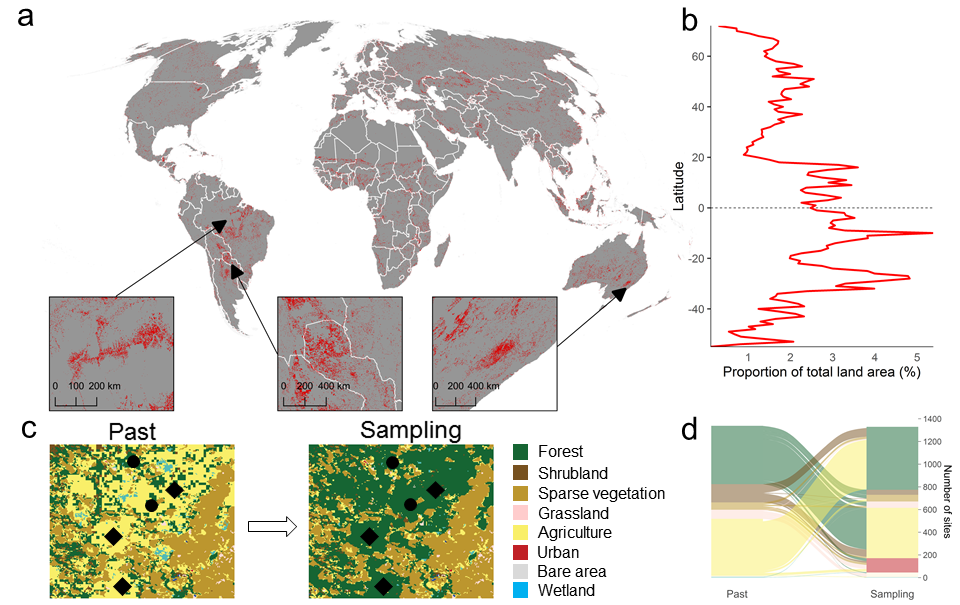
\includegraphics[width=1\textwidth]{chapter4/F01}
\caption{ (\textbf{a}) Global map depicting the grid cells of the ESA LC product that had $\geq 1$ land-cover change (red) in the period 1992 to 2015. Inset maps focus \textendash\ from left to right \textendash\ on the deforestation in the eastern Amazon basin, expanding soy plantations in Paraguay as well as shrubland loss in south east Australia. Map is projected in an equal-area Mollweide projection (\textbf{b}) Mean proportion of land with a land-cover change (in \%) in the period 1992 to 2015 averaged per 1\textdegree of latitude. (\textbf{c}) Example land cover maps of the past and at the time of biodiversity sampling for a single study. Black symbols indicate sites with (diamond) and without (circle) land-cover change. (\textbf{d}) Flow diagram showing the sequence of land cover of all PREDICTS sites with a past land-cover change. Colours as in \textbf{c}.  }
\label{F04_01}
\end{figure}
% -------------------------------------------- %

\subsection{Analyses}
\label{C04_03}

The statistical analysis for this study had two main aims. First, we aimed to quantify whether biodiversity measures were different at sites with a past land-cover change compared to sites without any land-cover change in the period 1992 to the start of biodiversity sampling. To do so, we fitted generalized linear mixed effects models (GLMMs) using Poisson distributed errors for species richness and a Gaussian error distribution for total abundance (log10 transformed) and the probability of an interspecific encounter (PIE, asin-squareroot transformed). Following previous studies \citep{Newbold2016,Jung2016} all models included the study identity and a spatial block of sampling design and additionally the ESA LC category at the time of biodiversity sampling as random intercept. We fitted separate GLMMs to assess the difference in local biodiversity measures between sites with and without (\textit{i}) a past land-cover change overall, (\textit{ii}) a categorical representation of the time passed since a land-cover change occurred (unchanged, \ie 0 years, or $\leq$ 5, 5-10, >10 years), (\textit{iii}) distinguishing sites with and without a past land-cover change by their land-cover sequence, for which we fitted separate GLMMs for each ESA LC category at the time of biodiversity sampling using the extracted sequence of land-cover (those with at least 10 sites to ensure robustness of coefficients) categories as fixed effect (Figure \ref{F04_01}\textbf{b}). Lastly (\textit{iv}) we fitted a GLMM using the ESA LC categories at the time of biodiversity sampling and as interacting covariate, human population density data from the global human settlement (GHS) project \citep{Pesaresi2013,Pesaresi2016}. We used data from the GHS project as it is available at a spatial (\textasciitilde 250m) and temporal (1975-2015) resolution that matches the resolution of the ESA LC data. All GLMMs were fitted using the ‘lme4’ package \citep[ver. 1.1-18-1,][]{lme4} in R \citep[ver. 3.5, ][]{RTeam2014}.

Second, we constructed global and national projections of biodiversity. We used the model described above (\textit{iv}) to project the mean coefficients of local biodiversity onto the global ESA LC map for the year 2015 only, which we resampled to \textasciitilde3 x 3 km spatial resolution by assigning the most dominant (‘modal’) LC value to each grid cell. All predicted estimates were transformed relative to the predicted estimate of a ‘forest’ site with zero human population density in the year 2015 \citep{Newbold2015}. Biodiversity sampling in the majority of PREDICTS sites (96.2\%) occurred between 2000 and 2013 and from the ESA LC maps of the years 2000 and 2015 we constructed a new global map for the year 2015 with each grid cell set to a unique categorical code of the sequence of land-cover (using Cantor’s pairing function). For each separate model (see \textit{iii} above) and unique sequence of land-cover categories a new spatial projection was created for those grid cells with the respective sequence. We then added (to the mean coefficients) those separate spatial projections to the projection of the global mean difference in local biodiversity for the year 2015 (see above), thus “updating” the projected difference in those grid cells only where a past land-cover change has occurred (see Appendix Figure \ref{SI04_01} for a schematic). Some land-cover sequences were not available among PREDICTS sites and here we used the global average impact (see model \textit{i}) in place of no better data available. Because of data limitations, we were also not able to investigate the impact of interactions between land-cover sequences and time passed on local biodiversity. Globally each grid cell has a different baseline level of local biodiversity \textendash\ \eg deserts being less species richness than shrublands \textendash\ and we followed \cite{Newbold2015} by weighting all grid cells using either a global layer of terrestrial vertebrate diversity \citep[summed range-of-occurrence maps for bird, mammal and amphibian species,][]{NatureServe2012,IUCN2016a} for species richness or a layer of global photosynthetic activity (average photosynthetic activity as measured by MODIS NDVI in the period 2000-2015) for total abundance and assemblage evenness \citep{Newbold2015}. 

Global biodiversity projections were visualized in a way that emphasises model uncertainty by supressing estimates with large uncertainty \citep{Correll2018}. We refitted the GLMM models using the ‘mgcv’ package \citep[ver. 1.8-24, ][]{Wood2011} because of their ability to obtain estimates of prediction uncertainty for hierarchical models. For each grid cell we predicted the standard error from the Bayesian posterior covariance matrix of the ‘mgcv’ model \citep{Wood2011} and used it to calculate the absolute error in the predicted difference of local biodiversity (known as mean absolute error or MAE). To use the MAE for visual suppression of uncertain projected estimates, we excluded the 1\% lowest and highest MAE estimates and furthermore normalized ($ \frac{(MAE - min(MAE) )}{(max(MAE) - min(MAE))} $) the MAE globally. To assess whether accounting for past land-cover sequences affects national biodiversity projections, we calculated the area-weighted relative mean difference in biodiversity at the national scale compared to a spatial projection where past land-cover changes are not taken into account ($\frac{x_{Sequence} -x_{without} }{|x_{without}|}$, where $x$ is the mean area-weighted predicted national difference in biodiversity). We differentiated countries into groups of high (black), middle (orange) or low (blue) income (according to \href{http://data.un.org}{http://data.un.org}) and assessed differences between those groups using ordinary analysis of variance (ANOVA) tests.

\section{Results}
\label{C04_03}

Across all sites in the PREDICTS database, 1326 sites had a single land-cover change in the years before biodiversity sampling compared to 13696 sites without any change (number of studies: 238). The greatest number of PREDICTS sites with a past land-cover change were forest covered (552), followed by agriculture (442) and urban covered (126) sites (Appendix Figure \ref{SI04_02}). Overall, sites with a past land-cover change had on average 5.3\% ($\pm$ 0.01 SE, p < 0.001) fewer species, 6.1\% ($\pm$ 0.03 SE, p < 0.001) fewer individuals and were 1.1\% ($\pm$ 0.01 SE, p = 0.217) less even compared to a site without a past land-cover change. With increasing time passed after a land-cover change occurred, local species richness and total abundance recovered to levels comparable to unchanged sites (Figure \ref{F04_02}). If a land-cover change occurred in the five years before biodiversity sampling, sites had on average 5.6\% ($\pm$ 0.01 SE, p < 0.001) fewer species and 8.5\% ($\pm$ 0.04 SE, p < 0.05) fewer individuals than sites without a land-cover change in the past. Compared to unchanged sites, assemblage evenness was not significantly different (1.6\% $\pm$ 0.01 SE, ns) for sites with a land-cover change less than 5 years ago but was significantly lower (4.4\% $\pm$ 0.01, p < 0.01) after 5 to 10 years had passed. 

% ---------------- Figure 2 --------------------- %
\begin{figure}[htb]
\centering
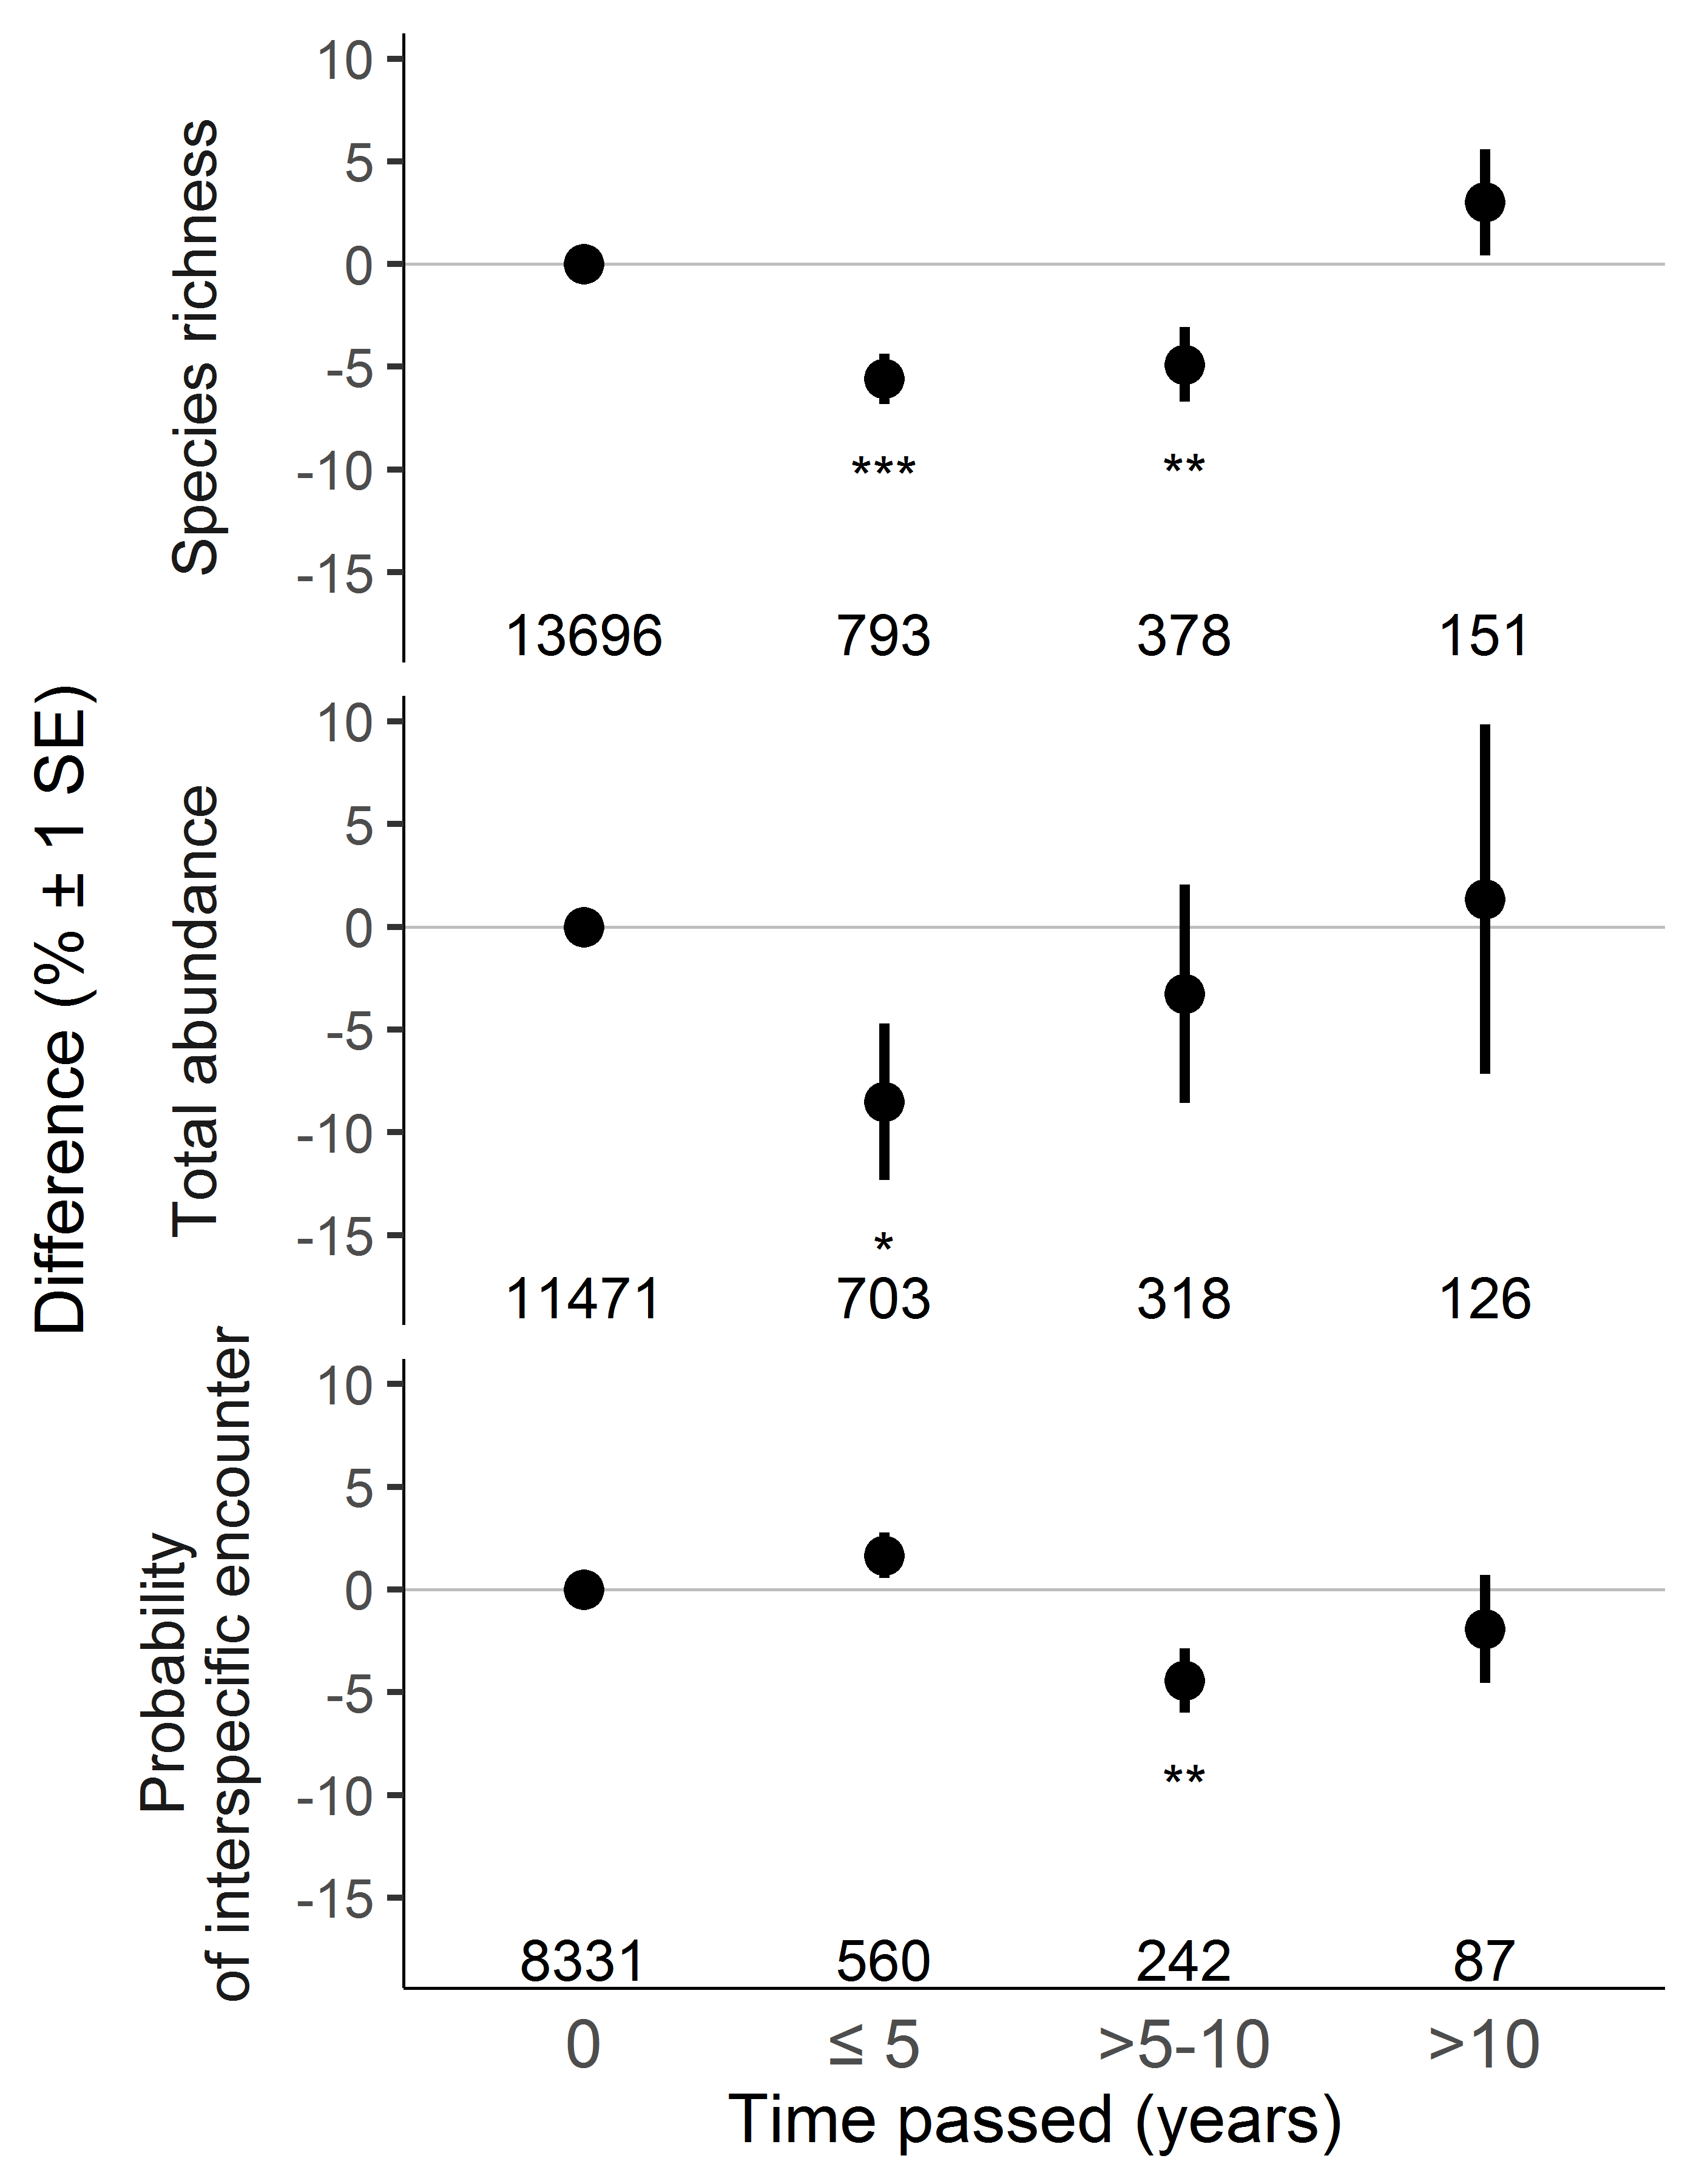
\includegraphics[width=1\textwidth]{chapter4/F02}
\caption{ Difference in local biodiversity measures between sites without (0) and sites with a past land-cover change that occurred $\leq$ 5 years, > 5-10 or over 10 years ago. The error bars show the predicted standard error and stars (*) indicate whether the difference was statistically significant (p < 0.05). The total number of sites is indicated. }
\label{F04_02}
\end{figure}
% -------------------------------------------- %

Local biodiversity varied between sites with and without a past land-cover change depending on past land-cover sequences (Figure \ref{F04_03}). The number of species (11.4\% $\pm$ 4 SE) and individuals (13.4\% $\pm$ 12.9 SE) of forest sites was lower if the site had been shrub covered before biodiversity sampling compared to forest sites without a land-cover change in the past (Figure \ref{F04_03}\textbf{a}), while the number of species was higher (17.4\% $\pm$ 5.51 SE) if the preceding land cover had been grassland. More species (10.83\% $\pm$ 5.51 SE) and individuals (26.1\% $\pm$ 15.1 SE) were found in previously forest covered sites compared to shrubland sites without a past land-cover change (Figure \ref{F04_03}\textbf{b}). The number of species and individuals in agricultural sites was lower if the preceding land cover was forest (8.81\% $\pm$ 2.1 SE for species and 6.93\% $\pm$ 6.9 SE for individuals) or shrubland (23.93\% $\pm$ 3.9 SE and 35.8\% $\pm$ 18.4 SE) compared to sites without a land-cover change in the past (Figure \ref{F04_03}\textbf{e}). Sites with urban land cover had in most cases higher number of species, individuals and assemblage evenness (up to 80.2\% $\pm$ 30 SE for abundance in agriculture, Figure \ref{F04_03}\textbf{f}) compared to urban sites without a past land-cover change, with only species assemblages in previously agricultural sites being less even (Figure \ref{F04_03}\textbf{f}).

% ---------------- Figure 3 --------------------- %
\begin{figure}[ht]
\centering
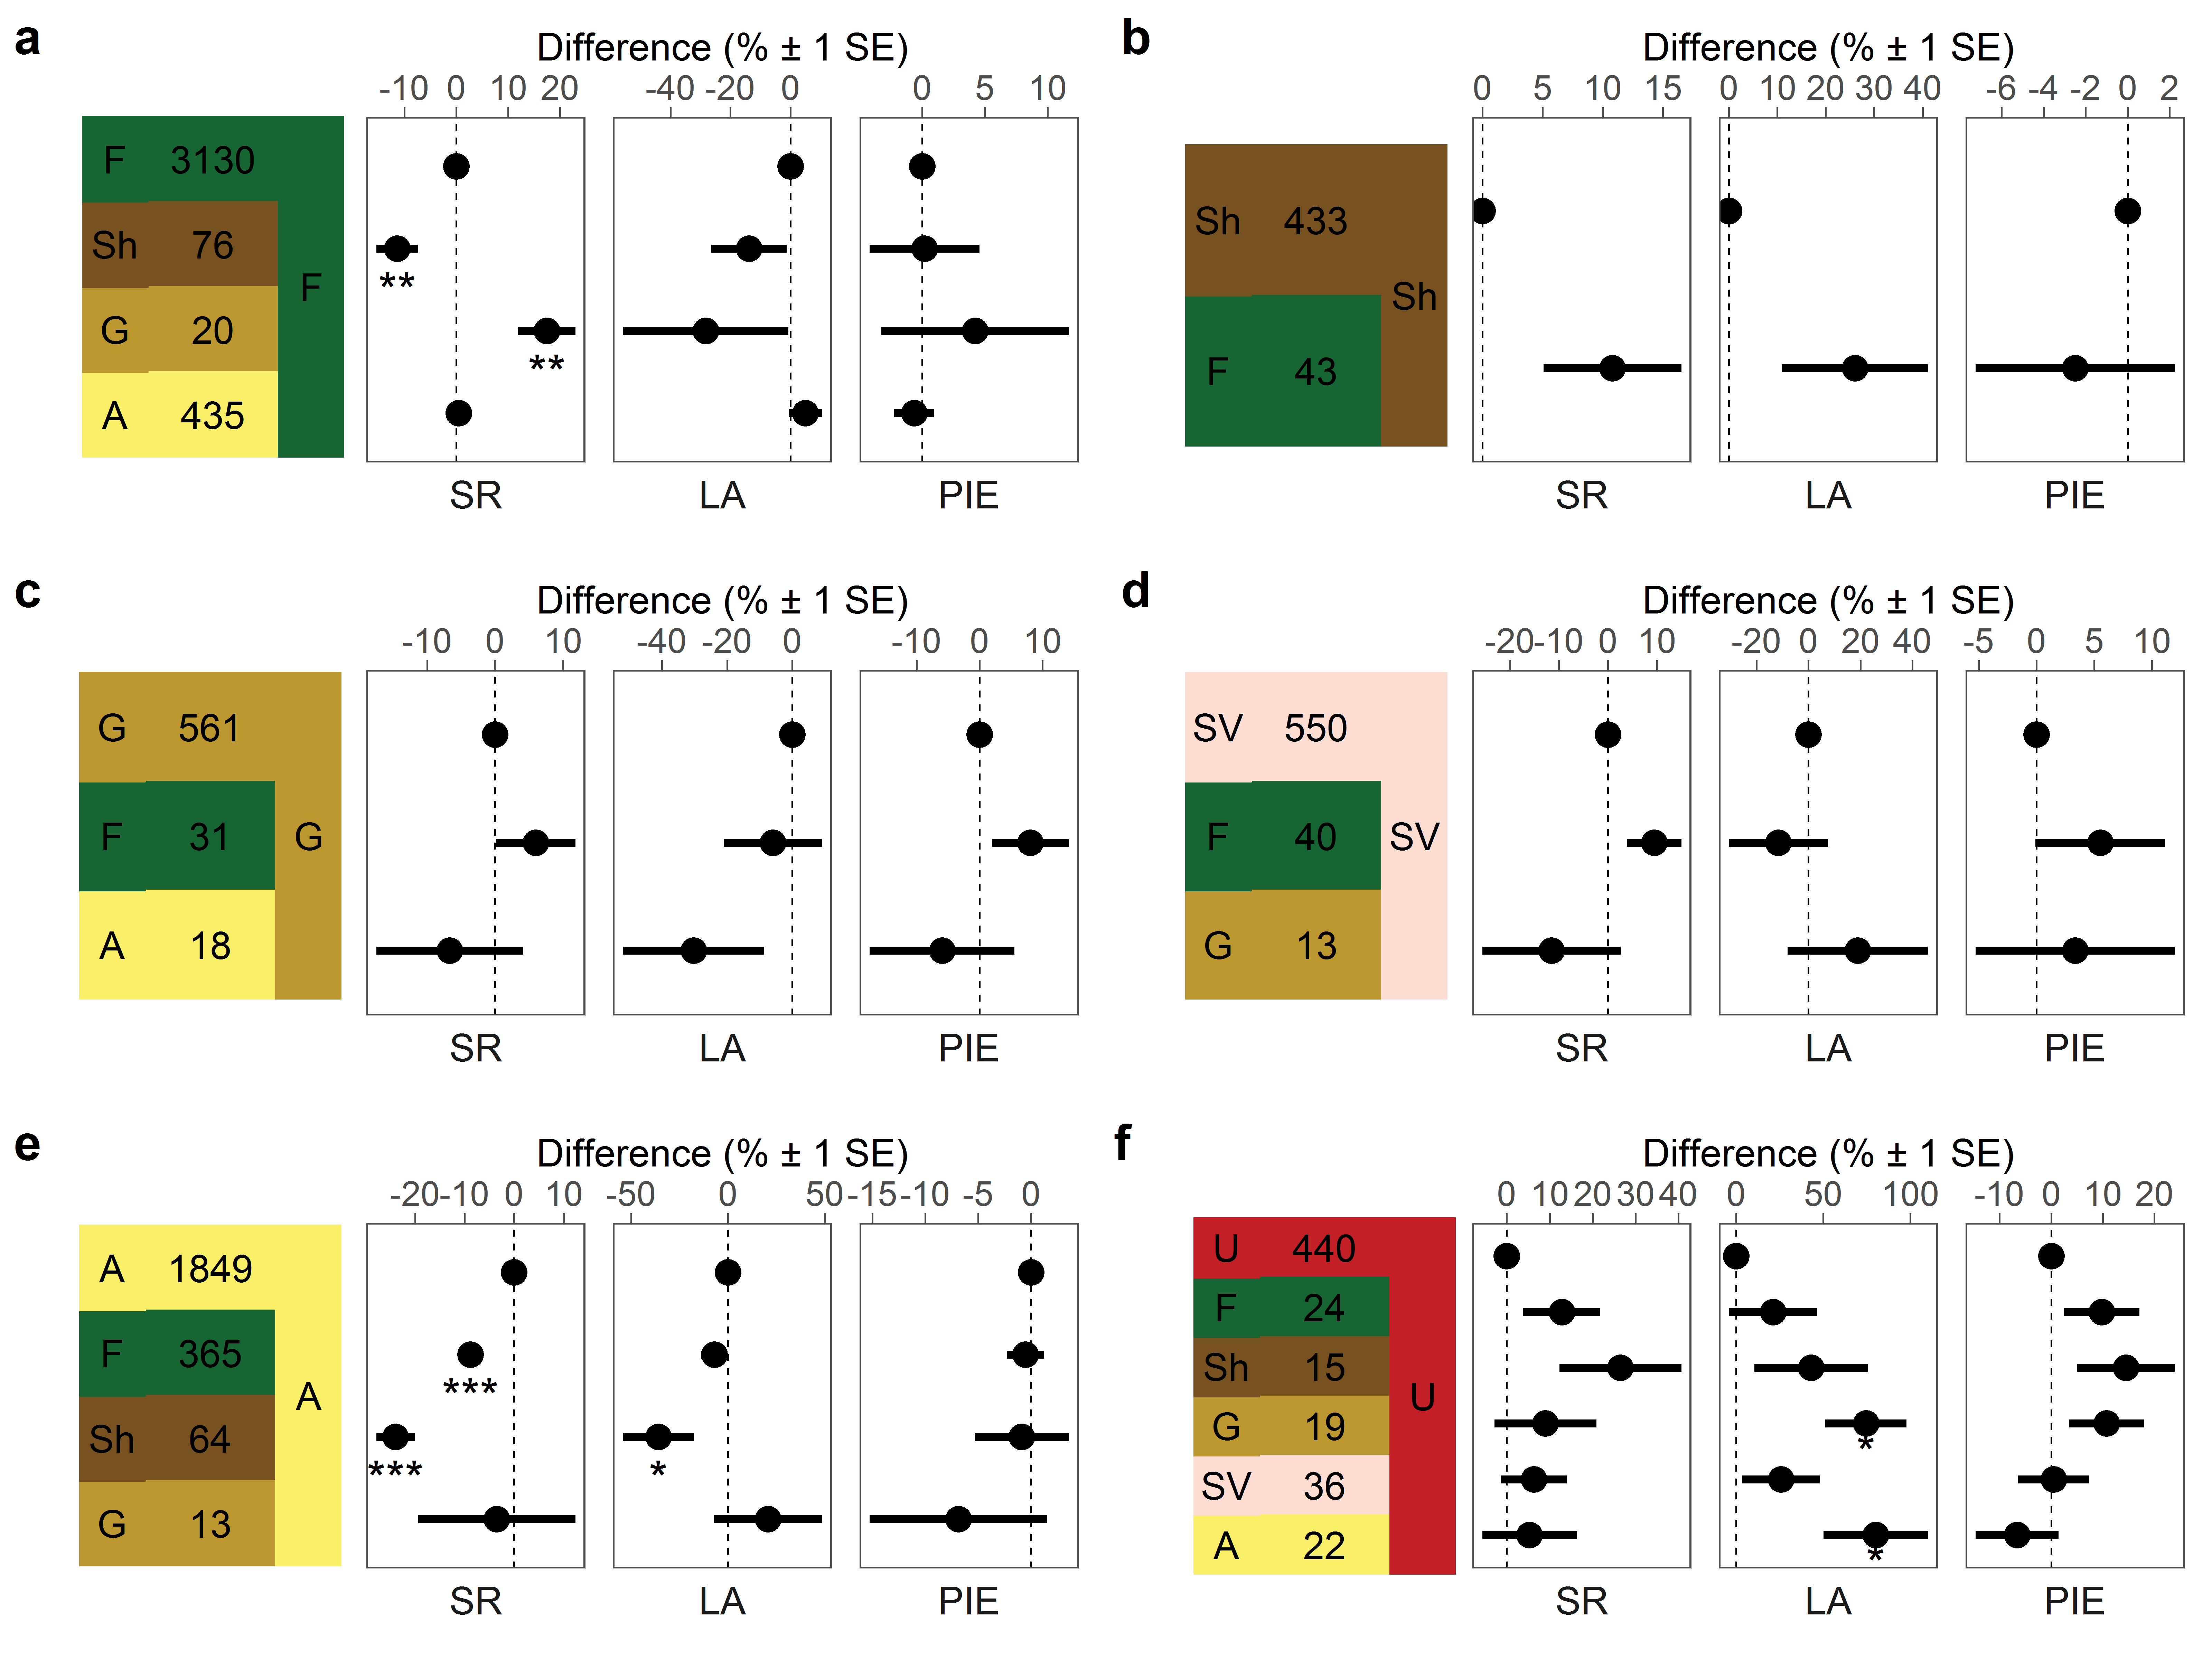
\includegraphics[width=1\textwidth]{chapter4/F03}
\caption{ Difference in local biodiversity measures between sites with varying sequences of land cover relative to sites without any past land-cover change (dotted line) in the period 1992 to biodiversity sampling start. Separate models were fitted for each biodiversity measure and land cover at the time of biodiversity sampling as indicated by colour and abbreviation, namely forest (F, \textbf{a}), shrubland (Sh, \textbf{b}), grassland (G, \textbf{c}), sparse vegetation (SV, \textbf{d}), agriculture (A, \textbf{e}) and urban (U, \textbf{f}). Abbreviations on the x-axis show the difference in local biodiversity (SR = Species richness, LA = Total abundance, PIE = Species assemblage evenness). Number of sites contributing to each fitted land-cover sequence are indicated. The error bars show the predicted standard error and stars (*) indicate whether the difference is statistically significant (p < 0.05).}
\label{F04_03}
\end{figure}
% -------------------------------------------- %

Local biodiversity varied globally with land cover in the year 2015 as estimated from spatial projections (Figure \ref{F04_04}\textbf{a}). Estimates of projected grid cells had a range from 41\% to 0\% fewer species, -10\% to 13.3\% fewer individuals and 30.3\% to 46.1\% less even assemblages. Globally projected differences in species richness had considerable uncertainty ranging between $\pm$ 0.1\% and $\pm$ 29\% MAE in the most extreme cases (grid cells with over 5.5\% MAE occurred in less than 1\% of all land grid cells). Informed by past land-cover sequences (Figure \ref{F04_03}), we found the predicted number of species to be up to 17.1\% lower or 20.1\% higher than estimates that do not take sequences of past land cover into account (Appendix Figure \ref{SI04_03}). This is especially the case for locations in the Amazon and Gran Chaco (Figure \ref{F04_01}\textbf{b}), where after \textendash\ accounting for land-cover change between 2000 and 2015 \textendash\ high losses of species are expected (Figure \ref{F04_04}\textbf{b}). Projections were created using human population density as spatial covariate and we found that a greater human population density increased species richness in sparse vegetation, agriculture and urban covered sites relative to forest covered grid cells, while total abundance increased with population density across all land-cover categories relative to forest covered grid cells (Appendix Figure \ref{SI04_04}).

% ---------------- Figure 4 --------------------- %
\begin{figure}[ht]
\centering
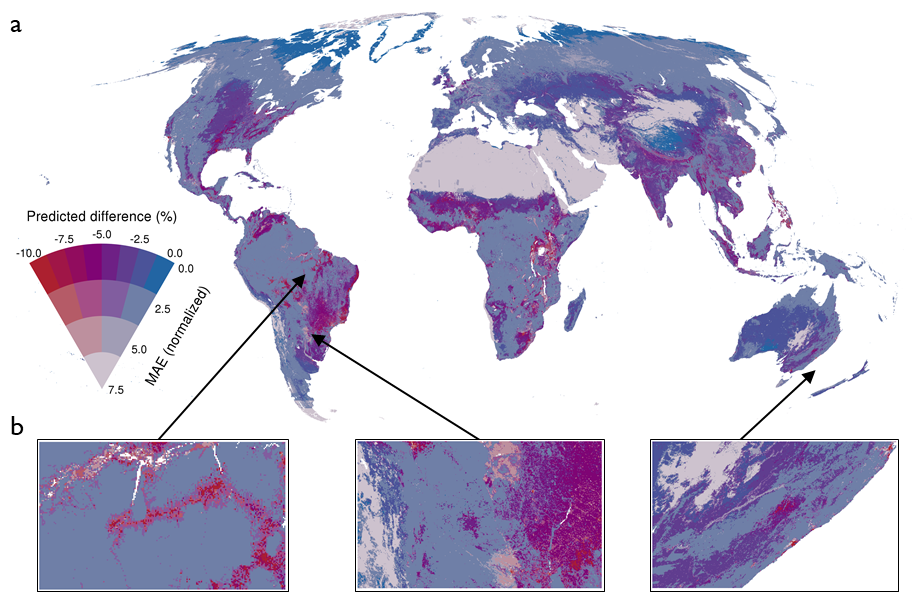
\includegraphics[width=1\textwidth]{chapter4/F04}
\caption{ (\textbf{a}) Global projection of the difference in local species richness with land cover \textendash\ relative to a forest site with zero human population \textendash\ and informed by land-cover sequences in the past. Projected estimates are visualized relative to their uncertainty (normalized mean absolute error (MAE) from the predicted difference), where values of higher uncertainty visually suppressed in hue. Most extreme values (lowest 1\% and highest 1\% percentile) were excluded from the visualization and are displayed as inland white colour. (\textbf{b}) shows examples (as in Figure \ref{F04_01}) how projections of local species richness loss differ because of prediction uncertainties and land-cover sequences. Inland white pixels are within the 1\% of highest estimates of projected species richness loss after accounting for past land-cover sequences. Map is displayed in a global equal-area Mollweide projection and aggregated (\textasciitilde 3000$m^2$) for this visualization. Predicted difference and uncertainty (unweighted) are in Appendix Figure \ref{SI04_03} individually. }
\label{F04_04}
\end{figure}
% -------------------------------------------- %
Land cover changes continue to influence biodiversity estimates at the national scale. On average 4.04\% $\pm$ 3.73 SD of land across all countries had a land-cover change relative to their total land area in the period from 2000 to 2015. Singapore with 31.7\%, Malawi with 17.7\% and Paraguay with 16.4\% had the highest proportion of land with a land-cover change in the period 2000 to 2015 (Appendix Figure \ref{SI04_05}). Although there were no significant differences in the proportion of land with a land-cover change among countries ($F_{2,201}$=0.477,p=0.621, Appendix Figure \ref{SI04_05}), considering past land-cover change affected biodiversity more in tropical, lower-income countries (Figure \ref{F04_05}, Appendix Figure \ref{SI04_06}-\ref{SI04_07}). The area-weighted difference in projected national biodiversity estimates \textendash\ relative to a projection that did not account for land-cover sequences \textendash\ was significantly lower in low income countries for species richness ($F_{2,200}$=9.131,p<0.001, Figure \ref{F04_05}), total abundance ($F_{2,198}$=13.48, p<0.001, Figure \ref{SI04_06}) and evenness ($F_{2,198}$=6.644,p<0.01, Appendix Figure \ref{SI04_07}).

% ---------------- Figure 5 --------------------- %
\begin{figure}[ht]
\centering
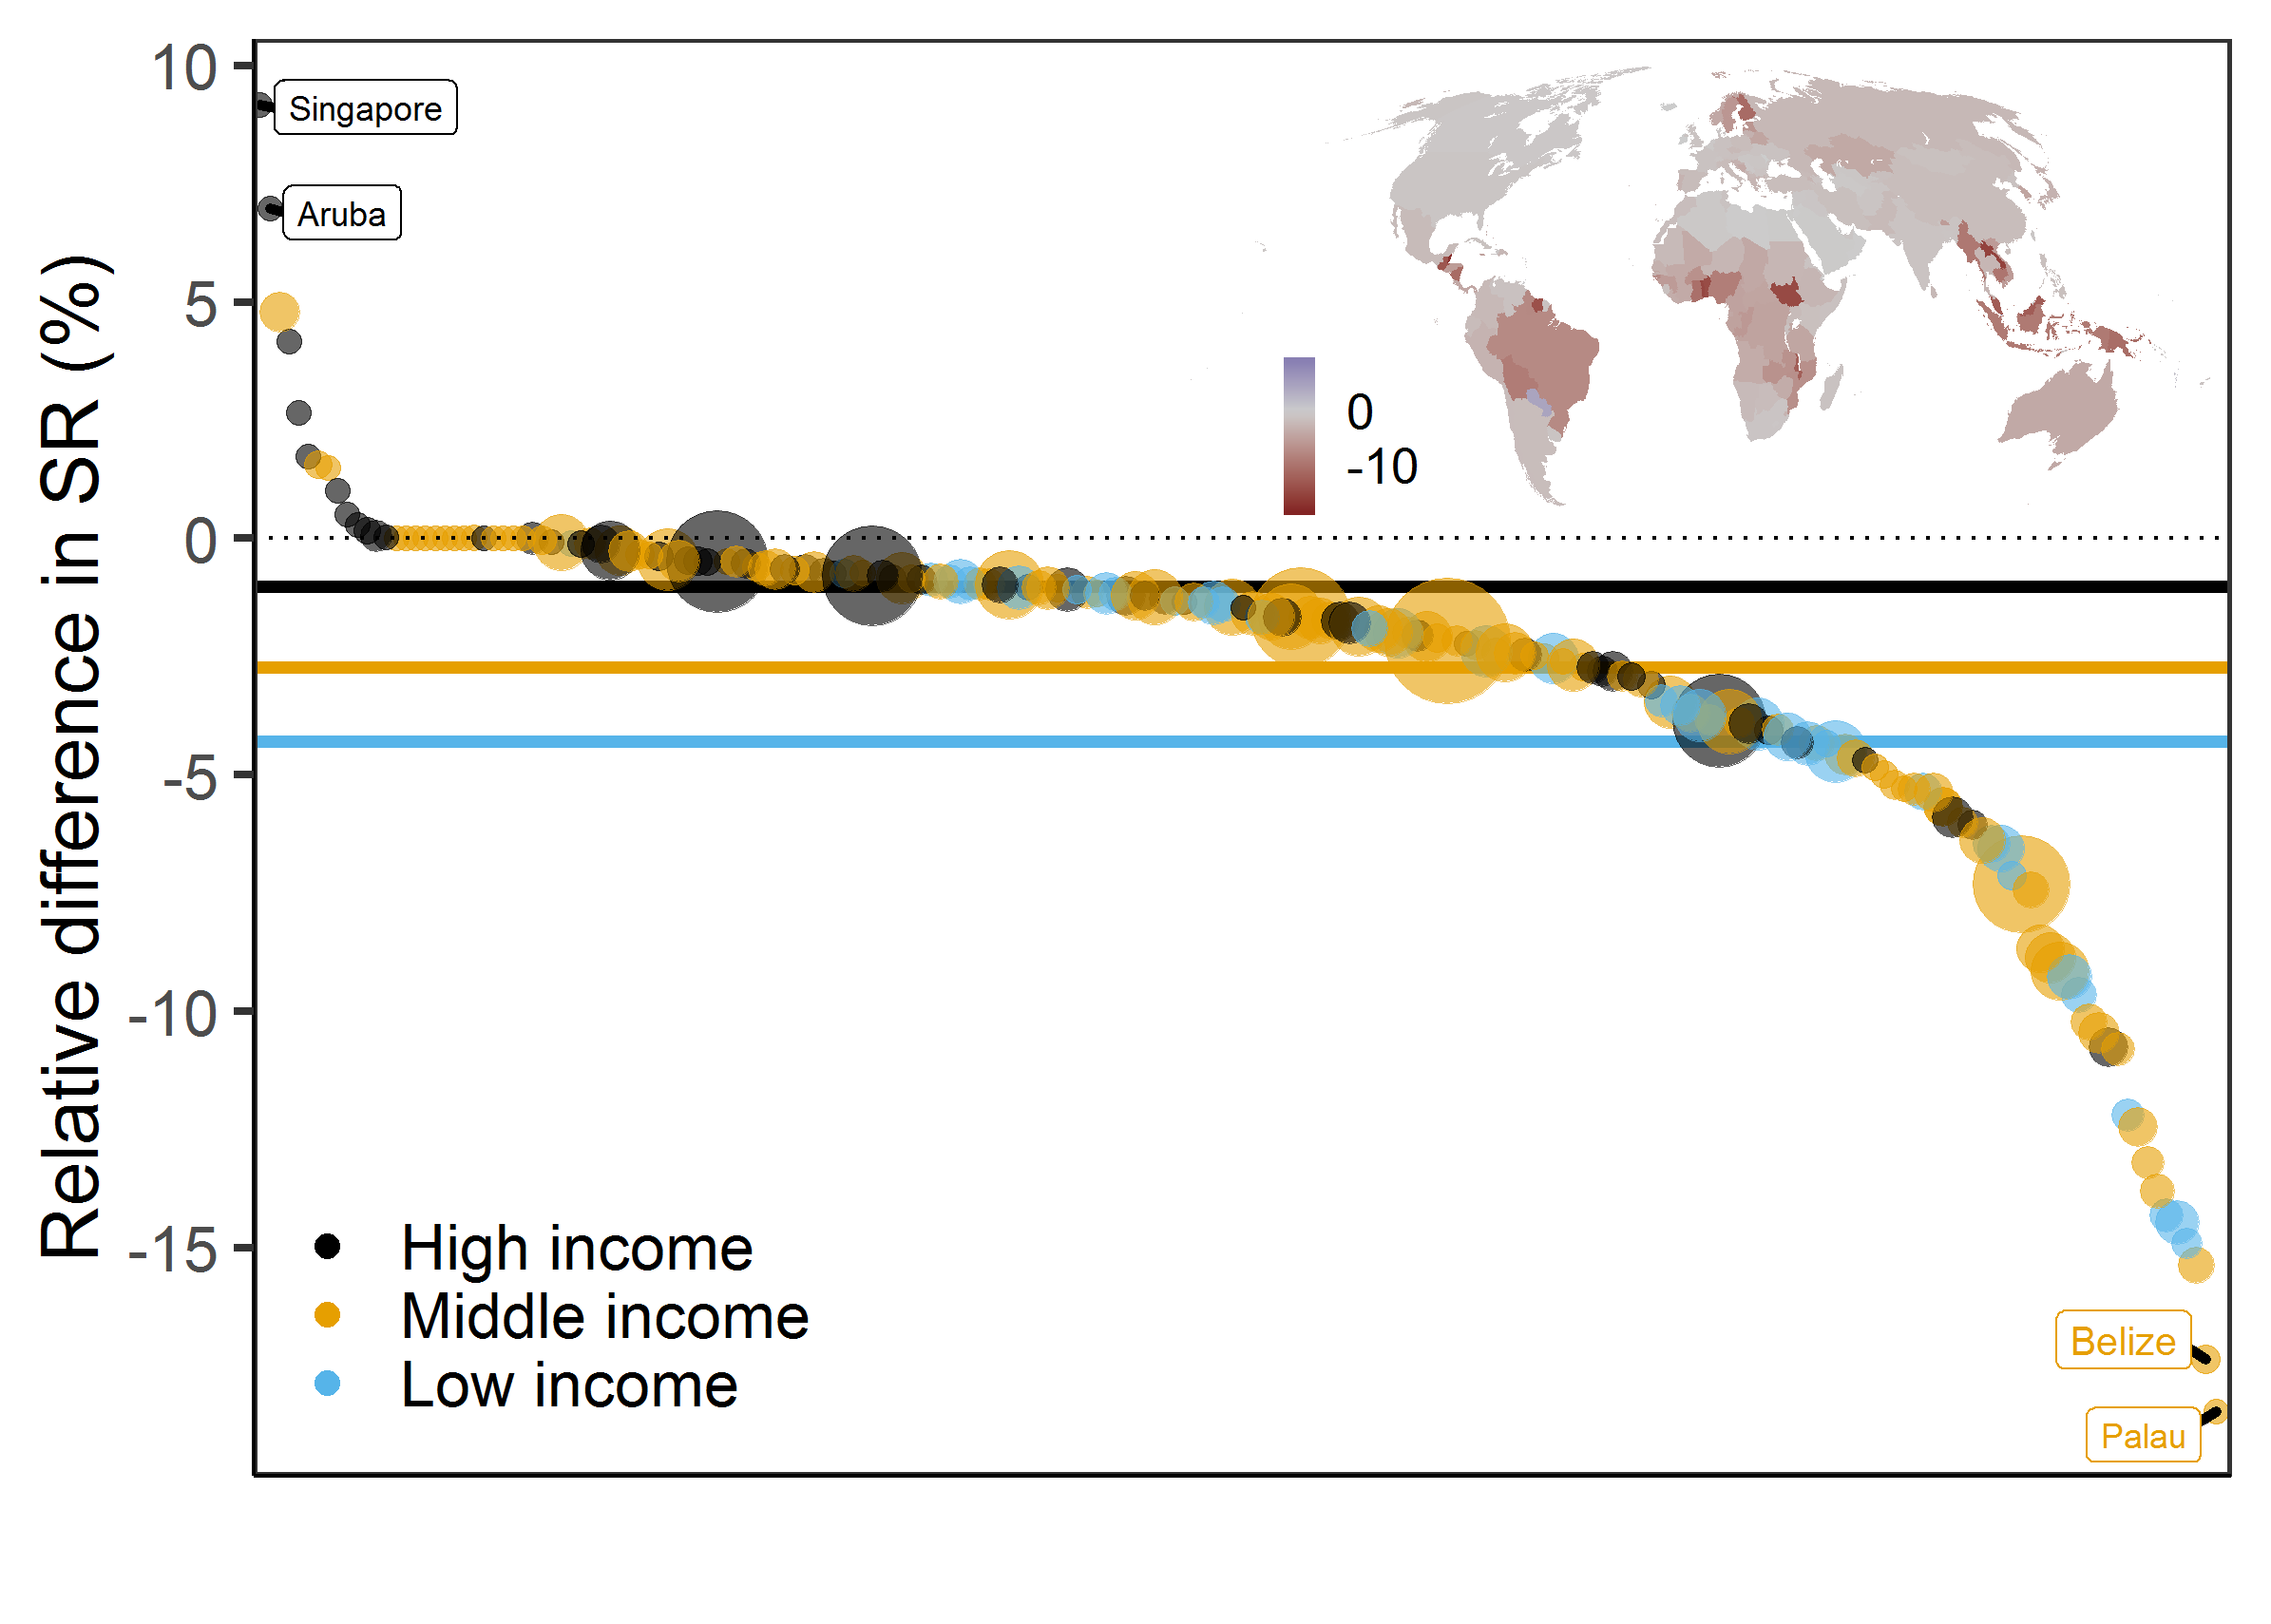
\includegraphics[width=1\textwidth]{chapter4/F05}
\caption{ Area-weighted relative difference \textendash\ compared to a projection where past land-cover sequences were not considered \textendash\ in mean national species richness (SR) from 2000 to 2015. Points represent the country-wide average in SR (area-weighted) with the size of the points scaled with land area (small to large). Colours indicate whether countries are considered high (black), middle (orange) or low (blue) income. Outlier countries and overall averages per income group (vertical lines) are indicated. Inset map shows the relative difference in SR from low (red) to high (blue) per country. Plots for total abundance and assemblage evenness are broadly comparable (Appendix Figure \ref{SI04_06}-\ref{SI04_07}). }
\label{F04_05}
\end{figure}
% -------------------------------------------- %

\section{Discussion}
\label{C04_04}

Biodiversity differs with attributes of past land-cover change \citep{Watson2014}. We found local biodiversity at sites with a past land-cover change to be on average lower than at sites without any land-cover change in the period 1992 to biodiversity sampling start. Local biodiversity recovered to levels comparable to sites without land-cover change after more than ten years had passed (Figure \ref{F04_02}). These results are in line with a previous study on the same biodiversity dataset that found abrupt land changes to consistently reduce local biodiversity (Chapter \ref{C03} in this thesis). We furthermore found that the impacts of land-cover change on biodiversity varied with different sequences of past land cover (Figure \ref{F04_03}) and that these impacts affect global (Figure \ref{F04_04}) and national (Figure \ref{F04_05}) biodiversity projections. We discuss how our results relate to those of previous studies and make recommendations how to incorporate lasting influences of past land-cover change into biodiversity projections.

\subsection{The influence of land-cover sequences on local, national and global biodiversity}
\label{C04_0401}

Depending on the sequence of land cover, local biodiversity estimates are considerably altered after a land-cover change. Forest covered sites, that were previously covered by agriculture, had about the same number of species and individuals as forest covered sites without a land-cover change in the period 1992 to biodiversity sampling start (Figure \ref{F04_03}\textbf{a}), which contrasts with findings of previous studies investigating the impact of an agriculture to forest transition on local biodiversity \citep{Bellemare2002,Hermy2007,Dyer2010}. It could be that many of the reference forest-covered sites had an agricultural history long before 1992 \textendash\ which we were unable to quantify using the ESA LC product \textendash\ potentially weakening the impacts of land-cover change as local biodiversity has already been altered before the start of satellite-based earth observation \citep{Ellis2010,McMichael2017}. A previous meta-analysis has shown that forests, which were previously covered by shrublands had on average lower species richness \citep{Bremer2010} and we found similar results with previously shrub covered sites, having on average 11\% fewer species and 14\% fewer individuals (Figure \ref{F04_03}\textbf{a}). In contrast, previously forest covered shrubland sites had on average 11\% more species and 26\% more individuals than a shrubland site without a past land-cover change (Figure \ref{F04_03}\textbf{b}). Likely these sites still support a high number of species typical at low vegetation height and structural complexity \citep{Chazdon2016}. 

In more anthropogenically altered land cover, a past land-cover change caused varying “biotic lag” effects (Figure \ref{F04_03}\textbf{e}-\textbf{f}). Urban sites with a past land-cover change had a higher number of species and individuals than sites without land-cover change (Figure \ref{F04_03}\textbf{f}). It could be that local biodiversity in these sites is inflated because of pending extinction debt and thus these sites likely have local extinctions of native species in the future \citep{Tilman1994,Kuussaari2009,Hylander2013}. This is supported by a global meta-analysis which has found that preceding land cover together with city age is one of the best predictors of (native) bird and plant occurrence in urban areas \citep{Aronson2014}. However, similar effects could not be observed for agricultural sites previously covered by forest or shrubland, where the number of species and individuals was on average lower compared to an agricultural site without a past land-cover change (Figure \ref{F04_03}\textbf{e}). One possible explanation could be that this pattern is mostly driven by (pollinating) invertebrates, which compose 64.8\% of all previously forest or shrub covered agricultural sites in our dataset. Pollinating invertebrates have previously been shown to have higher numbers of species and individuals in agricultural land compared to forests \citep{Winfree2009}. It should be mentioned that many of our findings could be rather imprecise given the low number of sites with a past land-cover change (Appendix Figure \ref{SI04_02}), which prevented us from robustly assessing the impact of land-cover sequences across taxonomic or functional groups \citep{Jung2018} or in interactions with other attributes of land-cover change such as time passed (Figure \ref{F04_02}). Nevertheless, these estimates are to our knowledge the first comprehensive and comparative assessment of the impact of past land-cover sequences on local biodiversity measures.

The consideration of past land-cover change can also affect global and national biodiversity projections (Figure \ref{F04_04},\ref{F04_05}). Although only 4.04\% of the terrestrial land surface globally had a land-cover change in the period 1992 to 2015 occurring predominantly in the global south (Figure \ref{F04_01}), which is in line with previous studies that analysed the spatial distribution and drivers of land-over change \citep{Curtis2018,Nowosad2018} and found the expansion of agricultural and pastural land to be the most likely cause \citep{Phalan2013}. Those areas are often globally irreplaceable for biodiversity \citep{Brooks2002,Laurance2014,Pimm2014}. Comparing national biodiversity projections with and without a consideration of past land-cover change, we find that a consideration of land-cover sequences led to even lower biodiversity estimates in most, but especially so in tropical and low-income countries (Figure \ref{F04_05}, Appendix Figure \ref{SI04_06}-\ref{SI04_07}). In those countries anthropogenically caused land-cover change is commonly linked to attempts to close yield-gaps in agricultural production \citep{Mueller2012a} or increase the output of export commodities \citep{Byerlee2014,Meyfroidt2018}. Our results indicated that not accounting for lagged effects of past land-cover change can cause an over- and/or underestimation of biodiversity change in global projections.

\subsection{Model and land cover data uncertainties in biodiversity projections}
\label{C04_0402}

There are several factors that need to be considered when our results are compared to those of previous studies \citep{Newbold2015}. The PREDICTS database was set up to compare biodiversity measures between sites of varying land-use and land-use intensity derived from study descriptions \citep{Newbold2015,Hudson2016}, while this study used remotely-sensed estimates of land cover. Land use and land cover are intertwined in a land system \citep{Lambin2006,Turner2007}, however not all differences between two PREDICTS sites can likely be explained by land cover (and human population density, Appendix Figure \ref{SI04_03}) alone. Differences in impact can arise because of inaccuracies in characterizing land cover \citep{ESA2017}, scale mismatches \citep{Estes2018} or local factors that mediate biodiversity responses to differences in land cover \citep{Jung2016}. Furthermore because of sampling size limitations, we were not able to incorporate other attributes of land-cover change that could be important in determining differences in local biodiversity \citep{Watson2014}, such as the frequency \citep{Watson2014,Griffiths2015} or magnitude of land-cover change (Chapter \ref{C03} in this thesis). Future studies should attempt to incorporate interactions between attributes of land-cover change into biodiversity projections, pending greater biodiversity and land-cover data availability.

Remotely characterizing land-use and/or land-cover at global extents is challenging \citep{VERBURG2011,Kuemmerle2013}. In this study we used time series (period 1992-2015) of remotely-sensed land cover instead of the modelled estimates (1500-2100) of land use and land cover \citep{Hurtt2011,KleinGoldewijk2016} used by previous studies \citep{Newbold2015,Newbold2016,DePalma2017}. Most of the terrestrial land surface has been altered by humans long before the availability of Earth observation data \citep{Ellis2010} and modelled estimates of land use and land cover change are often the only available data at global scales. However, these estimates are only available at coarse spatial resolution (\textasciitilde 10 $km^2$ at the equator) and are dependent on model assumptions and accompanied uncertainties \citep{Gaillard2010,KleinGoldewijk2013}, with previous independent validations having shown that they can misrepresent pre-industrial land use substantially \citep{Kaplan2017}. Remotely-sensed land-cover products, despite classification errors and thematic differences that can affect subsequent analyses \citep{Sexton2015,Estes2018}, remain some of the best directly measured estimates of global land cover, but not land use. Promising case studies have quantified proxies of land use for agricultural \citep{Estel2015}, pasture \citep{Rufin2015} or forest use intensity \citep{Pflugmacher2012} from time series of remotely-sensed data at the regional scale. We suggest that in order to improve future biodiversity models and projections, new time series of proxies of land use need to be developed at the global scale. 

\section{Discussion}
\label{C04_05}

This study investigated the impacts of past land-cover change \textendash\ differentiated by attributes such as time passed or the sequence of land cover \textendash\ on local biodiversity. We found local biodiversity to be significantly reduced shortly after a land-cover change but being able to recover with longer time passed (Figure \ref{F04_02}). Depending on the sequence of past land cover, local biodiversity either increased or decreased compared to sites without a land-cover change (Figure \ref{F04_03}). If those lasting influences of past land-cover change are ignored in global and national biodiversity projections, we find that they can considerably misrepresent projected biodiversity change, especially so in tropical and low-income countries (Figure \ref{F04_04},\ref{F04_05}). There are several ways to improve biodiversity projections beyond of what has been presented in this study. We emphasize the need to consider interactions between attributes of land-cover change such as between the time passed (Figure \ref{F04_02}) and land-cover sequences (Figure \ref{F04_03}), which might affect the estimated impacts on biodiversity given evidence from previous studies \citep{Chazdon2003,Martin2013}. The impacts of land-cover change could furthermore be estimated using before and after biodiversity measures \citep{DePalma2018} and time series of land cover could be useful to identify sites for resurveying local biodiversity (see discussion \ref{C06}) or to establish links with time series of biodiversity measures \citep{Dornelas2018}. Overall, our study highlights the usefulness of remotely-sensed time series of land cover for biodiversity projections and models, particularly in quantifying lasting impacts of past land cover change.

\clearpage
%\bibliography{content/04Chapter}

%\appendix
%\begingroup
%  % SI - Figure 1 Missing data
\begin{figure}[h]
\centering
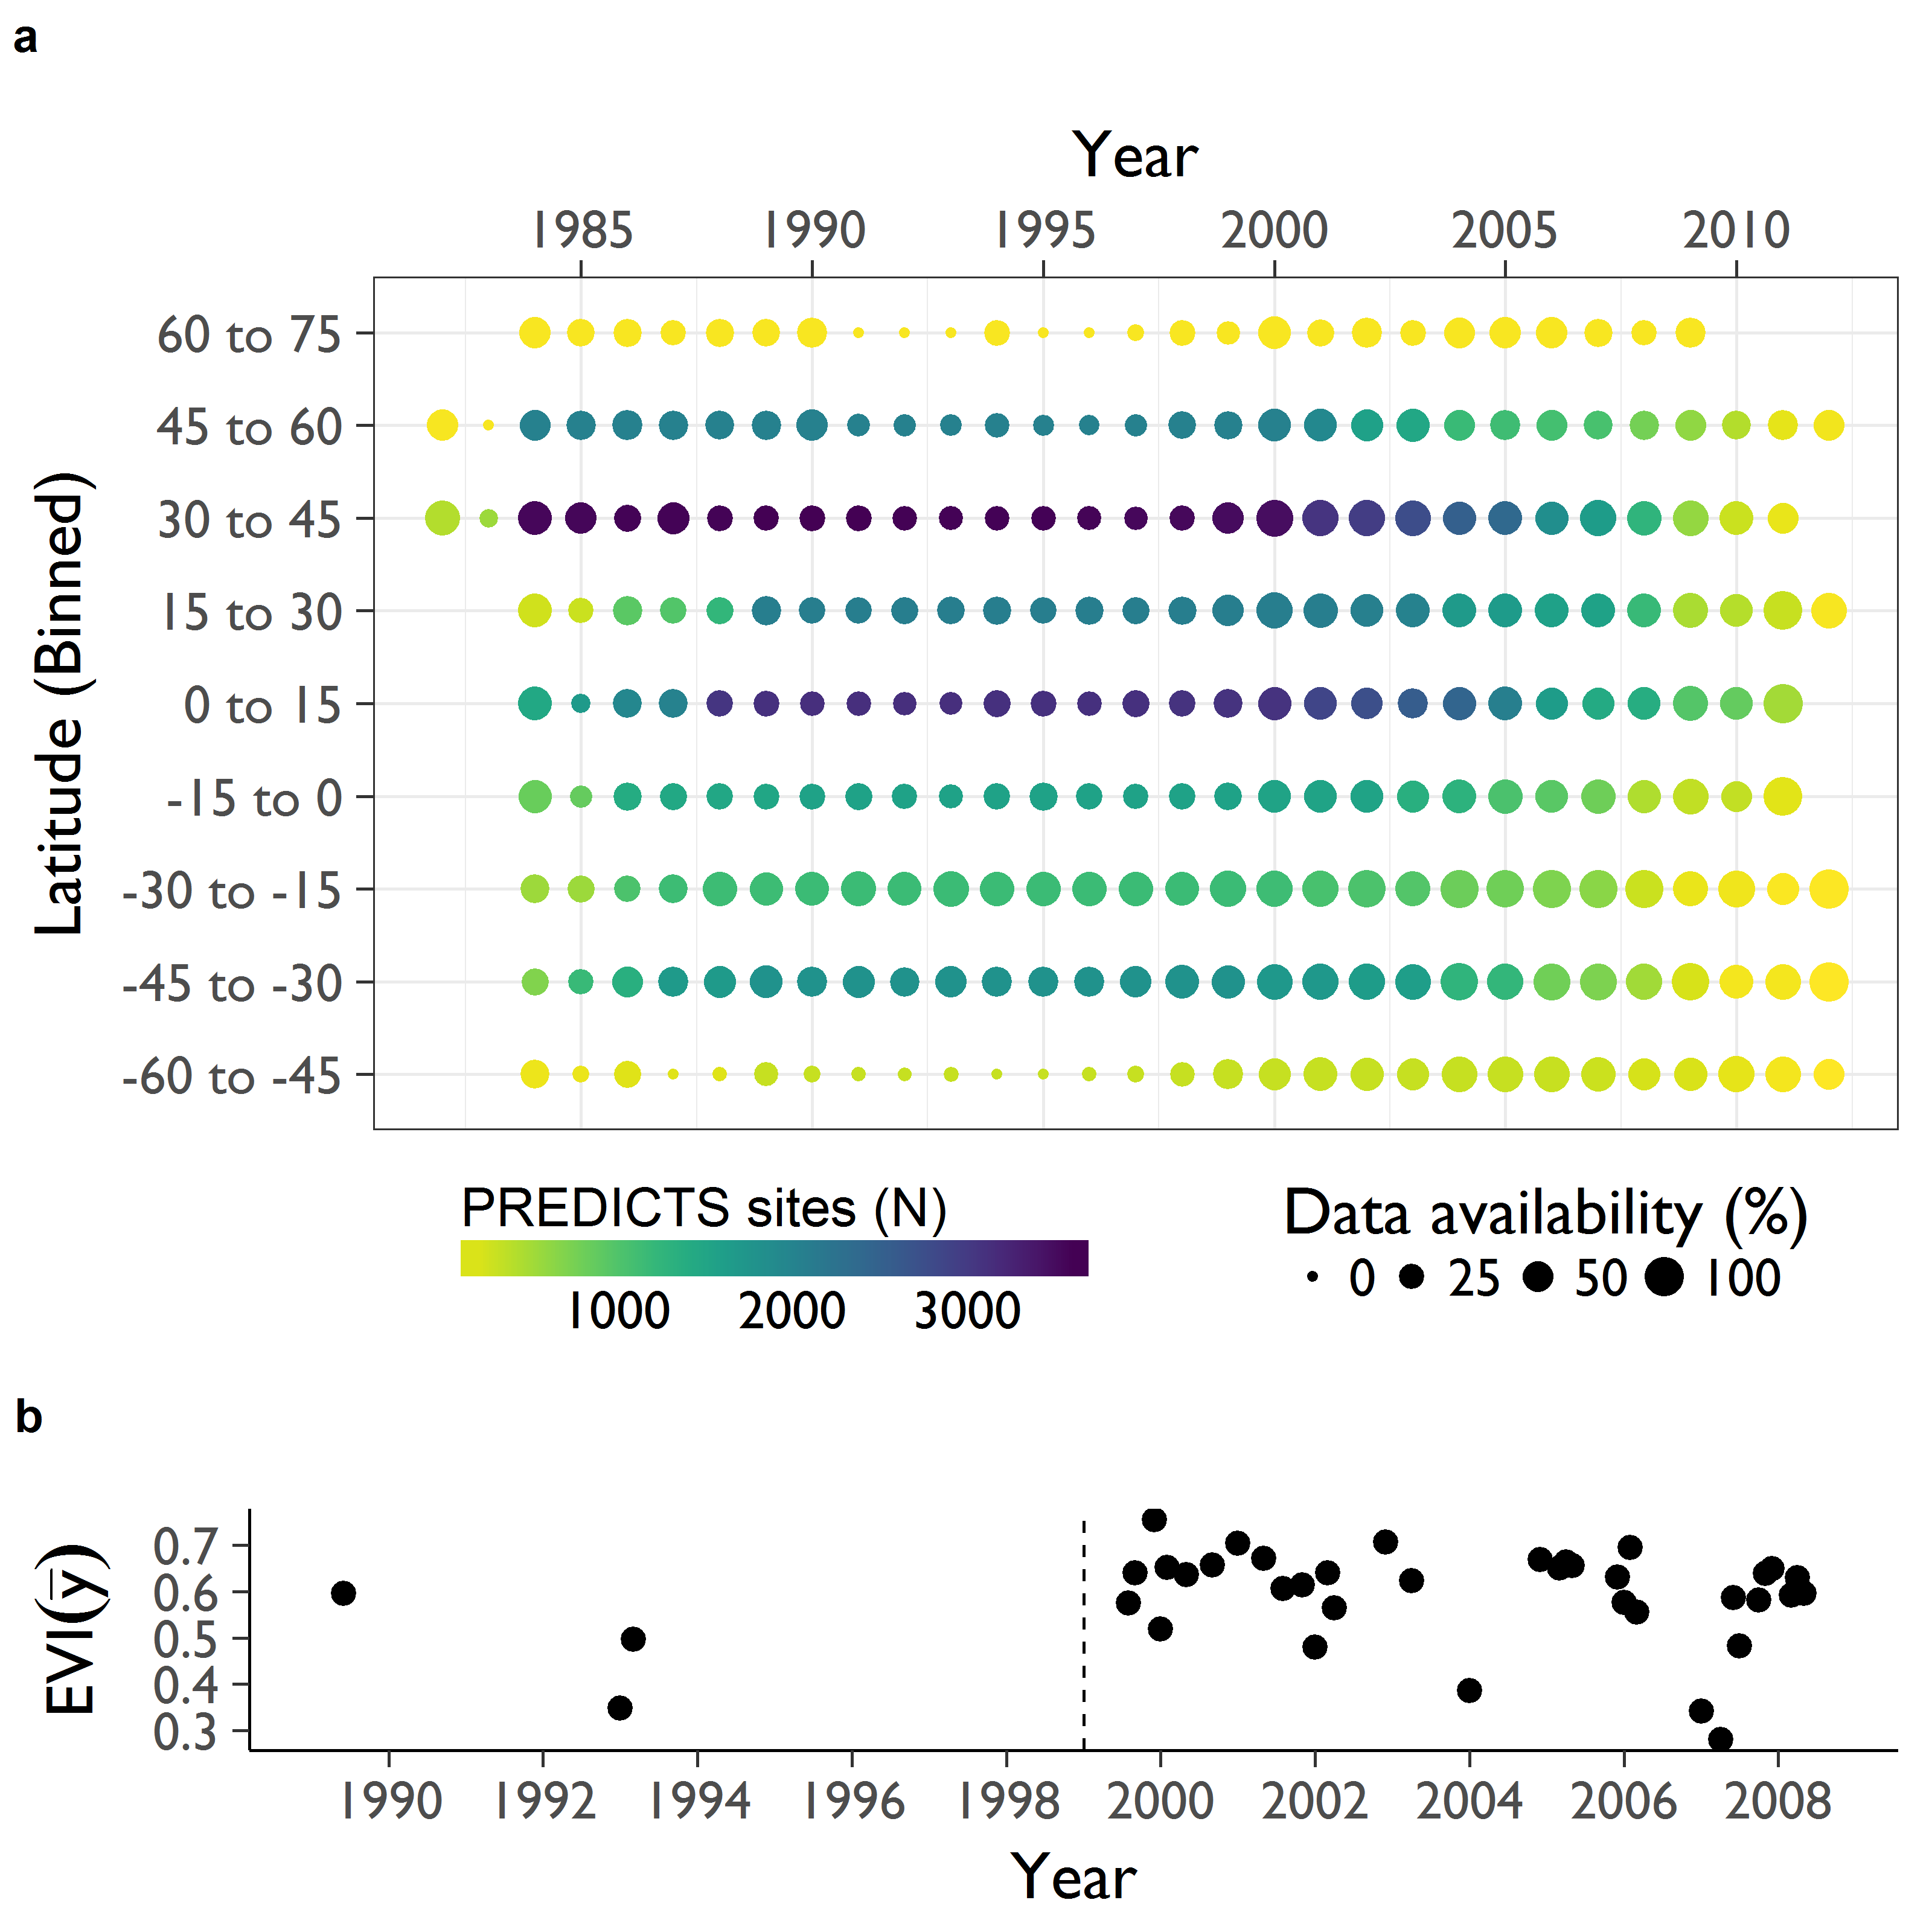
\includegraphics[width=1\textwidth]{chapter3/SI01}
\caption{ Average temporal distribution of Landsat data and an example times series of Landsat data. (\textbf{a}) Distribution of available Enhanced Vegetation Index (EVI) data in years covered by the Landsat missions. Points show the average monthly EVI data availability per year (0 to 12 months of data) across time series and PREDICTS sites grouped by 15\textdegree latitude bins. The size of points indicates the mean data availability (0 to 100\% with 100\% having 12 months of available data in a given year), while the colour shows the number of PREDICTS sites contributing to the mean (as PREDICTS sites were sampled in varying years). (\textbf{b}) Example time series for one PREDICTS site with a high proportion of missing data before 1999. In all analyses such time series were truncated to the period from 1999 onwards (indicated by the dashed line).}
\label{SI03_01}
\end{figure}

% SI - Figure 2 Binning
\begin{figure}[h]
\centering
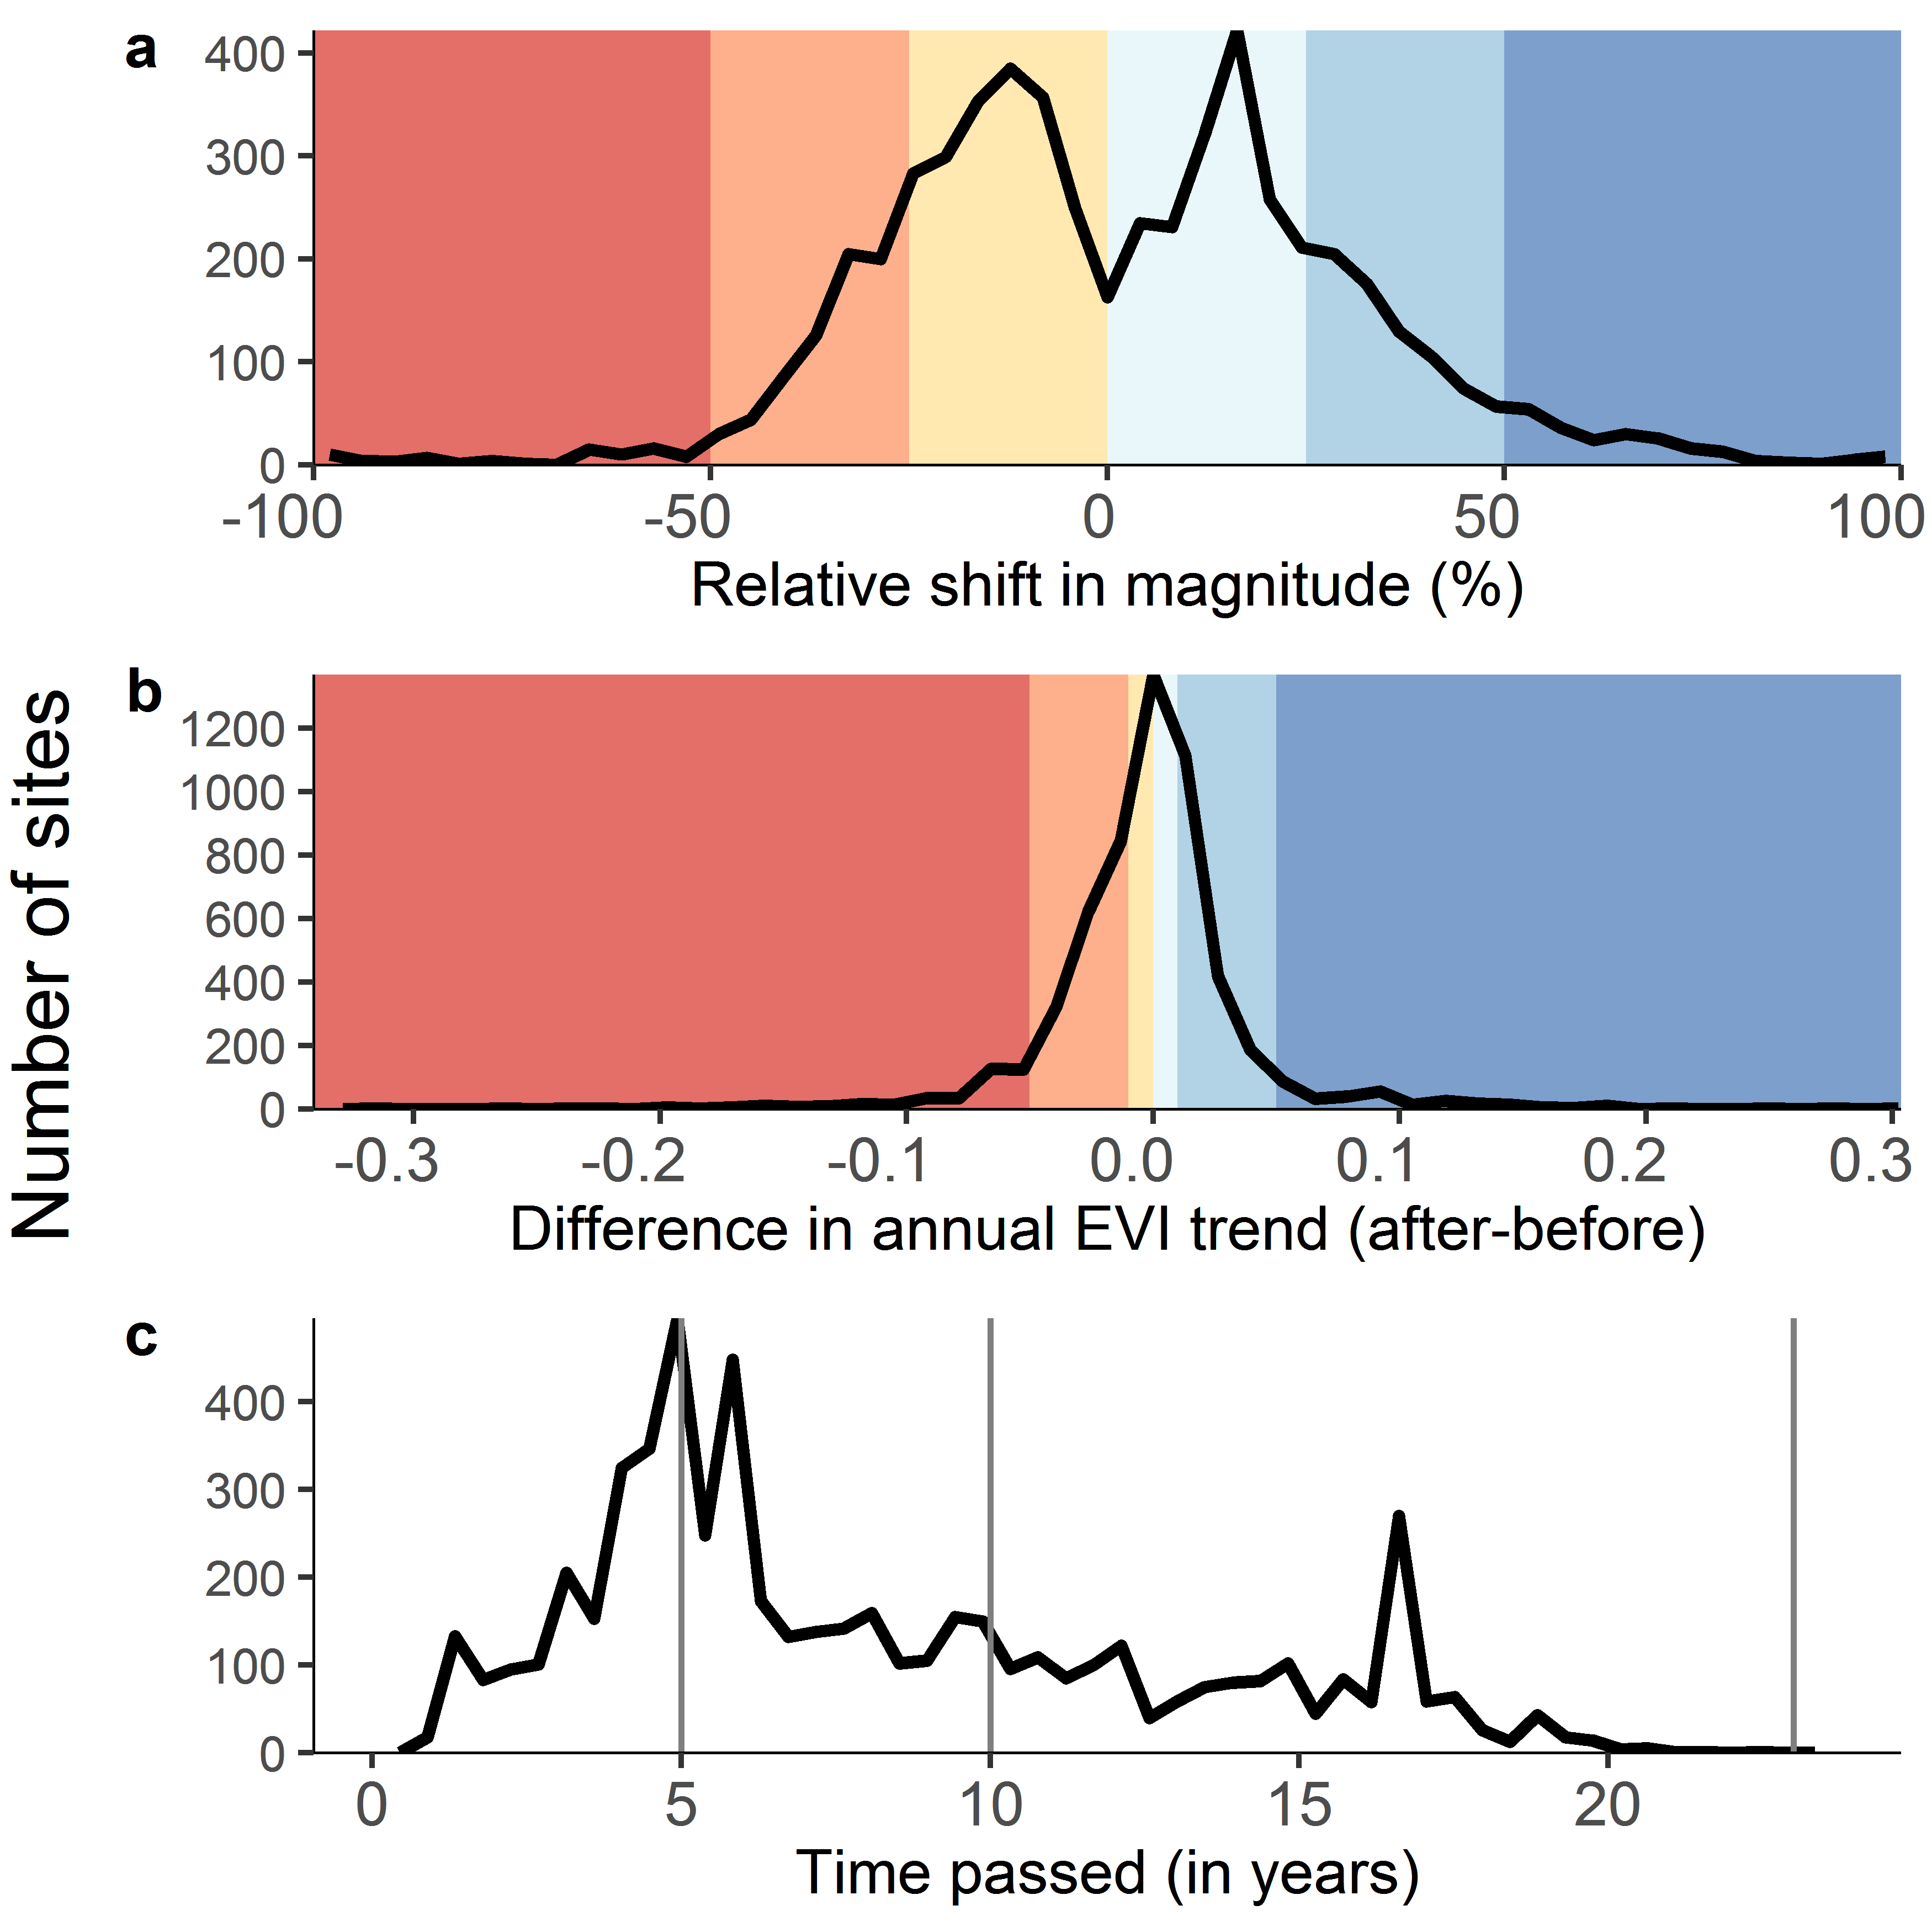
\includegraphics[width=1\textwidth]{chapter3/SI02}
\caption{ Number of sites with abrupt land change per attribute. Number of sites (black line) per attribute of abrupt land change with (\textbf{a}) the relative shift in magnitude, (\textbf{b}) the shift in trend as difference in annual EVI trend, and (\textbf{c}) the time passed between abrupt land change and biodiversity sampling. Background colours in (\textbf{a}) and (\textbf{b}) indicate the binning into six groups for shifts in magnitude (> 50\%, > 25\% to $\leq$ 50\%, and $\leq$ 25\% EVI loss [$---$ to $-$] or gain [$+++$ to $+$]), and in trend (0.01, 0.05, and > 0.05 annual negative [$---$ to $-$] to positive [$+++$ to $+$] EVI trend differences). Gray lines in (\textbf{c}) delineate bins of time passed ($\leq$ 5 years, > 5 and $\leq$ 10 years, and >10 years). Colours as in Figure \ref{F03_02}.}
\label{SI03_02}
\end{figure}

% SI Table 1------ %
% From here https://www.tablesgenerator.com/
\begin{table}[]
\centering
\caption{Number of PREDICTS sites and studies with an abrupt land change. Shown as either a change in magnitude (columns) and/or change in trend (trend). Symbols as in Figure \ref{F03_02}. }
\label{SIT03_01}
\begin{tabular}{@{}lllllllllll@{}}
                                          &                                           & \multicolumn{7}{c}{\textbf{Shift in magnitude}}                                                                                                                                                                    &                               &                             \\
                                          &                                           & \textbf{- - -}             & \textbf{- -}                & \textbf{-}                   & \textbf{0}                    & \textbf{+}                   & \textbf{+ +}                & \textbf{+ + +}              & \textbf{Total sites}          & \textbf{Studies}            \\ \cmidrule(l){3-11} 
                                          & \multicolumn{1}{l|}{- - -}                & 2                          & 8                           & 192                          & NA                            & 73                           & 26                          & 22                          & \cellcolor[HTML]{EFEFEF}323   & \cellcolor[HTML]{C0C0C0}57  \\
                                          & \multicolumn{1}{l|}{- -}                  & 7                          & 281                         & 642                          & NA                            & 497                          & 158                         & 53                          & \cellcolor[HTML]{EFEFEF}1638  & \cellcolor[HTML]{C0C0C0}175 \\
                                          & \multicolumn{1}{l|}{-}                    & 7                          & 88                          & 256                          & NA                            & 231                          & 154                         & 53                          & \cellcolor[HTML]{EFEFEF}789   & \cellcolor[HTML]{C0C0C0}184 \\
                                          & \multicolumn{1}{l|}{0}                    & NA                         & NA                          & NA                           & 10102                         & NA                           & NA                          & NA                          & \cellcolor[HTML]{EFEFEF}10102 & \cellcolor[HTML]{C0C0C0}358 \\
                                          & \multicolumn{1}{l|}{+}                    & 9                          & 102                         & 399                          & NA                            & 410                          & 205                         & 49                          & \cellcolor[HTML]{EFEFEF}1174  & \cellcolor[HTML]{C0C0C0}237 \\
                                          & \multicolumn{1}{l|}{\textbf{+ +}}         & 47                         & 172                         & 342                          & NA                            & 465                          & 254                         & 86                          & \cellcolor[HTML]{EFEFEF}1366  & \cellcolor[HTML]{C0C0C0}224 \\
\multirow{-7}{*}{\textbf{\rotatebox{90}{Shift in trend}}} & \multicolumn{1}{l|}{\textbf{+ + +}}       & 12                         & 137                         & 47                           & NA                            & 34                           & 12                          & 31                          & \cellcolor[HTML]{EFEFEF}273   & \cellcolor[HTML]{C0C0C0}56  \\
                                          & \multicolumn{1}{l|}{\textbf{Total sites}} & \cellcolor[HTML]{EFEFEF}84 & \cellcolor[HTML]{EFEFEF}788 & \cellcolor[HTML]{EFEFEF}1878 & \cellcolor[HTML]{EFEFEF}10102 & \cellcolor[HTML]{EFEFEF}1710 & \cellcolor[HTML]{EFEFEF}809 & \cellcolor[HTML]{EFEFEF}294 &                               &                             \\
                                          & \multicolumn{1}{c|}{\textbf{Studies}}     & \cellcolor[HTML]{C0C0C0}34 & \cellcolor[HTML]{C0C0C0}135 & \cellcolor[HTML]{C0C0C0}246  & \cellcolor[HTML]{C0C0C0}358   & \cellcolor[HTML]{C0C0C0}263  & \cellcolor[HTML]{C0C0C0}171 & \cellcolor[HTML]{C0C0C0}83  &                               &                            
\end{tabular}
\end{table}
% ------ %

% SI - Figure 3 Cross-correlations
\begin{figure}[h]
\centering
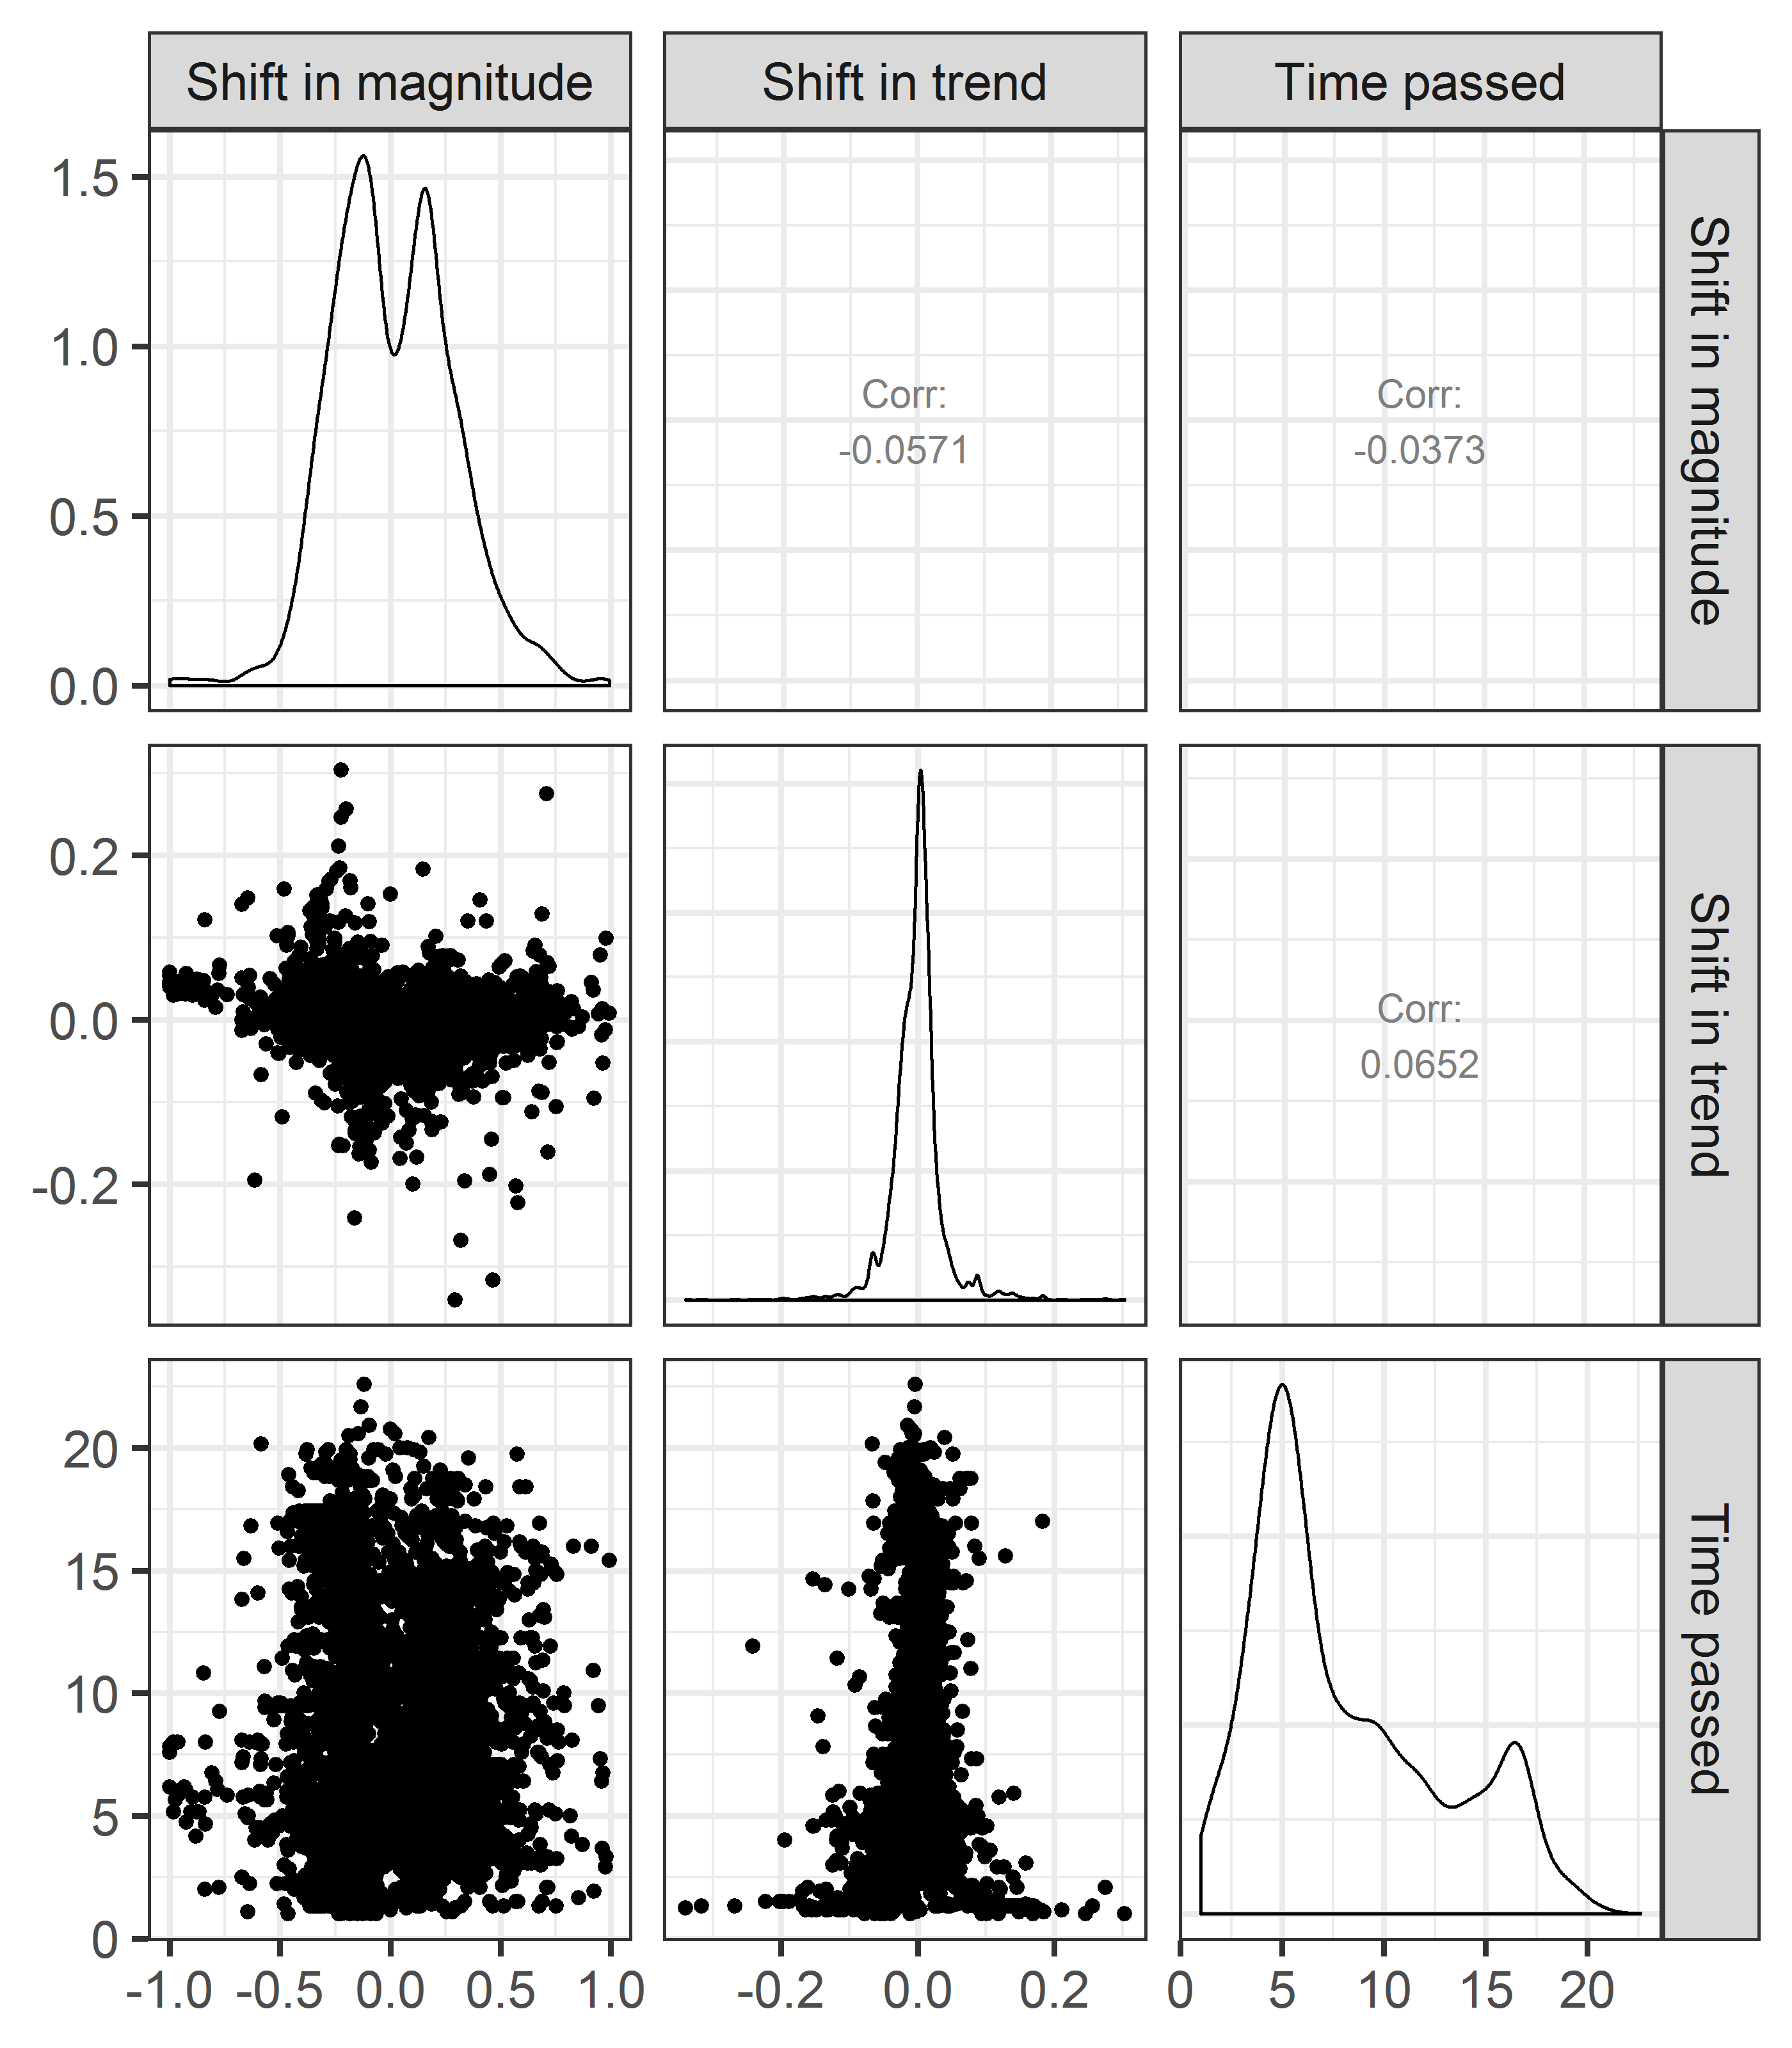
\includegraphics[width=1\textwidth]{chapter3/SI03}
\caption{ Correlations between attributes of abrupt land change. Showing shifts in magnitude, trend and time passed (see Methods). The lower facets show a point density plot, the upper facets the Pearson correlation coefficient between pairs of attributes and the diagonal a density plot.}
\label{SI03_03}
\end{figure}

%\endgroup

 %Land sequence piece
  %\chapter{Landscape-wide land changes correlate with, but rarely explain local bird diversity change}
%\addcontentsline{toc}{chapter}{Chapter 3}
%\markboth{}{Impacts of past abrupt land change on local biodiversity globally}
\label{C05}

There is an ongoing debate whether biodiversity at local scales is declining and what might drive this change. Land changes are suspected to impact local biodiversity change. However, there is little evidence across spatial and temporal scales and for multiple functional groups of species, thus limiting our understanding of the causes of local biodiversity change. Here we investigate whether landscape-wide land changes, opposed to those at the local scale, are driving local bird diversity change. We link time series of 34 years of breeding bird survey (BBS) data (1984-2017) at 2745 routes across the continental United States of America with remotely-sensed satellite imagery (\textasciitilde30m resolution) from the Landsat missions. Specifically, we assessed for each year what proportion of the landscape surrounding the BBS routes had a land change \textendash\ defined as abrupt shift in magnitude or trend of photosynthetic activity as detected by the Breaks for Additive Seasonal and Trend (BFAST) algorithm \textendash\ and tested whether large proportions of concomitant or preceding landscape-wide land changes explain changes in bird diversity, quantified as either geometric mean of relative abundance (GM) or progressive Bray-Curtis index (pBC). We found that the GM was negatively and the pBC positively correlated with a large proportion of land changes in the wider landscape. Furthermore, the consideration of preceding \textendash\ instead of concomitant \textendash\ landscape-wide land changes explained on average more variation in bird diversity change. Overall, landscape-wide land changes failed to explain most of the variation in local bird diversity change for most BBS routes regardless if bird diversity change is differentiated by functional groups or geographic regions. This study is one of the first studies attempting to link land and biodiversity change. It highlights the influence of preceding and concomitant land change on biodiversity and makes suggestions for promising directions of future research.  

\section{Introduction}
\label{C05_01}

Ongoing human alteration of the Earth surface causes changes in biodiversity across scales \citep{Gibson2011,Murphy2014,Newbold2015}. Globally, about 32\% of all known vertebrate species show decreasing population sizes and range contractions \citep{Ceballos2017,WWF2018} with reported species extinction rates being several times higher than expected naturally \citep{Brooks2002,Pimm2014}. Yet, any change in biodiversity is scale and measure dependent \citep{Sax2003,Chase2013} and, perhaps surprisingly, there is still a debate whether local \textendash\ opposed to global \textendash\ biodiversity is truly changing \citep{Thomas2013,McGill2014}. 

A number of global meta-analyses demonstrated that some biodiversity measures, notably species richness, have not changed at the local scale \citep{Vellend2013,Vellend2017,Dornelas2014}. However, these results have been questioned, particularly on whether the data are spatially and temporally biased \citep{Gonzalez2016} or if sites with and without land change were differentiated \citep{Cardinale2018}. This raises the question whether changes on land can explain changes in local biodiversity measures across space and time. 

Present differences on land influence local biodiversity globally. Previous studies found local biodiversity to be consistently reduced at sites with more intensively used land \citep{Murphy2014,Newbold2015,Alroy2017}, where on average 13.6\% fewer species and 10.7\% fewer individuals were observed compared to undisturbed primary vegetation \citep{Newbold2015}. However, these analyses relied on spatial comparisons of local biodiversity and therefore do not capture temporal biodiversity change. In addition, they ignored the influence of past land changes \citep{Perring2018,Jung2018} and did not consider landscape-wide land changes, which can influence local biodiversity \citep{Tscharntke2012,Turner2015,Miguet2015}. 

Local biodiversity is influenced by the variability of resources, such as food or nesting material, or through ecological processes, such as migration or fear of predation, at the landscape scale \citep{Hanski2000,Chase2003,Turner2015,Fernandez2016}. However these influences are not static and landscapes are constantly changing because of natural and anthropogenic factors \citep{Pickett1985,Manning2009,Turner2015}. Previous studies have shown that landscape-wide land changes may have a lasting influence on local biodiversity through ‘biotic lag’ effects \citep{Metzger2009,Ewers2013}. Yet, most studies focussed on small geographic regions and changes in forest cover \citep{Rittenhouse2010} and did not investigate general impacts of landscape-wide land changes on local biodiversity across spatio-temporal scales. A lack of data on local biodiversity and landscape-wide land change has so far prevented comparative assessments \citep{DePalma2018}.

Increasing availability of satellite imagery enables the assessment of land change at broad spatial and temporal scales \citep{Kennedy2014,Pasquarella2016}. Long-running satellite missions, such as Landsat, provide one of the best sources to monitor land-surface conditions \citep{Kennedy2014,Vogelmann2016,Hermosilla2018,Song2018}. Time series of land-surface conditions, such as photosynthetic activity, can measure intra- and inter-annual vegetation dynamics \citep{Pettorelli2005,Fisher2006} and specific algorithms have been developed to detect land changes as changes in photosynthetic activity \citep{Verbesselt2010,Zhu2017}. Land changes can be differentiated by attributes \citep{Watson2014}, such as abrupt shifts in magnitude, causing an immediate loss or gain of vegetation \citep{DeVries2015b}, or shifts in trend, causing either greening or browning over time \citep{DeJong2013,Muller2014}. These attributes can be robustly quantified at the landscape scale and linked to changes in local biodiversity.

Birds are one of the best surveyed taxonomic groups globally. Local biodiversity change quantified from repeated breeding bird surveys (BBS) has been widely studied \citep{Harrison2014,Pardieck2018}. Previous studies have shown that changes in bird diversity are dependent on the specific biodiversity measure     considered \citep{Schipper2016,Jarzyna2017} and are often non-linear \citep{Gutzwiller2015,Barnagaud2017}. Bird diversity change also varied spatially \citep{Harrison2014,Jarzyna2017} with many birds of particular functional traits, such as migratory or grassland dependent species, declining in developed countries \citep{Fewster2000,Sanderson2006,Stanton2018}. Land changes are most likely a driving factor of these declines \citep{Harrison2014,Harrison2016}, and yet most studies investigated only spatial correlations between remotely-sensed attributes of land change and local bird diversity \citep{Rowhani2008,Goetz2014,Hobi2017}. Notably \cite{Rittenhouse2010} found bird assemblage composition to be altered in landscapes with more “disturbed forests”, which they assessed using remotely-sensed time series. However, to our knowledge, no previous study has investigated whether landscape-wide land changes correlate with and explain changes in local bird diversity.

Consequently, this study hypothesizes that (\textit{i}) changes in local bird diversity are driven by landscape-wide land changes varying by land change attributes, (\textit{ii}) local bird diversity change can best be explained by past land changes, and (\textit{iii}) the explanatory power of landscape-wide land changes on local bird diversity change varies across geographic regions and functional groups of bird species. We combine 34 years (1984–2017) of annual BBS records collected at sites across the continental United States of America with time series of medium-high resolution (nominal \textasciitilde30m) satellite imagery from the Landsat missions. Using Breaks for Additive Seasonal and Trend (BFAST), a generic change detection algorithm, we detect abrupt shifts in magnitude (immediate gain or loss in photosynthetic activity) and trend (greening or browning) of photosynthetic activity in the landscape surrounding each BBS route. Non-linear spatio-temporal models were used to correlate the proportion of changing land in the wider landscape with changes in local bird diversity.
 %Bird piece
  %\chapter{General discussion and synthesis}
%\addcontentsline{toc}{chapter}{Chapter 6}
%\markboth{}{Thesis Synthesis}
\label{C06}

\section{Summary of main findings}
\label{C06_01}

The overarching goal of this thesis was to investigate how local biodiversity is impacted by land changes in the past and whether those impacts vary with key attributes of land change (\eg magnitude, frequency, time passed or sequence), across taxonomic groups, and geographic regions. I found past differences in land-surface conditions to be more important in explaining local species assemblage composition than present differences (Chapter \ref{C02}). Depending on attributes of land change, local species richness and total abundance were reduced, and assemblage composition altered after an abrupt land change (Chapter \ref{C03}) but were often able to recover to levels comparable to unchanged sites. Using the same biodiversity data, I found local biodiversity measures to decrease following past land-cover change and that attributes of land-cover change influence local, national and global biodiversity estimates differently (Chapter \ref{C04}). Chapters \ref{C02}-\ref{C05} assessed whether past land changes are correlated with spatial differences in local biodiversity at one point in time, however the impacts on biodiversity change \textit{per se} were not assessed. The results in chapter \ref{C05} indicated that past and concurrent landscape-wide land changes are correlated with but explain on average little variation in local bird diversity change. Overall these results demonstrate the pervasive impacts land changes can have on local biodiversity globally. In the following I discuss the implications of these results and directions for future research.

\subsection{Generalisability and application of findings}
\label{C06_0101}

In this thesis, I attempted to establish links between local biodiversity data (Projecting Responses of Ecological Diversity In Changing Terrestrial Systems [\textbf{PREDICTS}] \textendash\ \cite{Hudson2016}; United States Breeding Bird Survey [\textbf{BBS}] \textendash\ \cite{Pardieck2018}) and estimates of land change quantified from remotely-sensed satellite data globally (Figure \ref{F01_01}). This allowed me to address three important knowledge gaps.

First, most previous broad-scale studies only considered superficially \textendash\ if at all \textendash\ land changes in the past \citep{Alkemade2009,Murphy2014,Newbold2015} and corresponding biotic lag effects on local biodiversity \citep{Dullinger2013,Hylander2013}. Throughout the thesis and regardless of how past land changes were quantified (Chapter \ref{C02}-\ref{C05}), I discovered a consistent pattern that land changes in the past on average influenced local biodiversity measures and altered species assemblage composition, often more so than concurrent differences of land-surface conditions (Chapter \ref{C02} \& \ref{C05}). This implies \textendash\ not surprisingly given existing evidence of lasting influences of past land change on biodiversity \citep{Foster2003,Ewers2013,Perring2015} \textendash\ that previous broad-scales syntheses \citep{Murphy2014,Newbold2015,Alroy2017} likely underestimated the impacts of land change on local biodiversity. 

The second main gap this thesis addressed is the explicit consideration of attributes of land change. Land changes can be diverse and difficult to quantify and compare \citep{Kleyer2007}. Theoretical frameworks, such as the one developed by \cite{Watson2014}, distinguish land changes by a set of key attributes (\eg magnitude, frequency, time passed or sequence) with clear ecological relevance. Local biodiversity measures were considerably reduced following land changes with large magnitude (Chapter \ref{C03} \& \ref{C05}), \eg clear cutting of forested land or urbanization, which can act as disturbance \citep{Scheffer2001,Scheffer2003} reducing ecosystem stability \citep{Pimm1984,Hautier2015} and local biodiversity in concurrent and future years. In addition, the cumulative frequency of land changes (Chapter \ref{C02} \& \ref{C05}) can also influence biodiversity change, which \textendash\ together with magnitude impacts \textendash\ can be applied to improve predictions of biodiversity change \citep{Ewers2009,Ewers2013} and to establish linear and non-linear thresholds after which biodiversity change tends to accelerate \citep{VanderHoek2013,Gutzwiller2015}. Moreover, the results indicate that local biodiversity measures can \textendash\ on average \textendash\ recover to levels comparable of unchanged sites (Chapter \ref{C03} \& \ref{C04}), which is an important finding given that biodiversity recovery from past land changes is of major biodiversity conservation concern globally, especially as more and more land is secondary vegetation \citep{Chazdon2003,Jones2018}. Lastly, this thesis found that impacts of past land-cover change differed depending on the sequence of land cover (Chapter \ref{C04}), extending our knowledge on these impacts relative to previous studies that investigated only specific land-cover sequences or were based on very few estimates \citep{Foster2003,Bremer2010,Watson2014}.

Third, the influence of past land change on local biodiversity was previously unknown across geographic regions, taxonomic groups and biodiversity measures. I demonstrate how remotely-sensed estimates of land change can be robustly linked to local biodiversity data. Some attributes of land change, \eg time passed \citep{Martin2013,Fu2017} and magnitude \citep{Shackelford2017}, have been investigated previously in broad-scale syntheses. However, those studies lacked the taxonomic and geographic breadth, had small sample sizes \textendash\ 14 studies in the case of \cite{Shackelford2017} \textendash\ and were predominantly based on species richness only, which can be a misleading measure of biodiversity \citep{Su2004,Hillebrand2017}. The results in this thesis demonstrate that past land changes continue to influence local biodiversity globally and across multiple taxonomic groups and measures of local biodiversity (Chapter \ref{C02}-\ref{C05}). Furthermore, by using satellite-based instead of study-derived estimates of land change, the results presented in this thesis can easily be verified, repeated or build on by future studies. 

\subsection{Limitations of the presented results}
\label{C06_0102}

This thesis relies exclusively on a remote-sensing based characterization of land change. The definition of land change recognizes that land-use and/or land-cover cannot easily be separated \citep{Turner2007}. For instance, the observed differences in land-surface conditions in chapter \ref{C02} could be caused by changes in land use and/or land cover, with the exact driver being unknown. Land change can be driven by natural \textendash\ rather than anthropogenic \textendash\ factors and I did not attempt to identify the drivers of land change \citep{Curtis2018}. However, it could be that land changes caused by natural factors \textendash\ \eg precipitation anomalies, flooding, etc. \textendash\ compared to anthropogenically caused land changes \textendash\ \eg agricultural intensification or urbanisation \textendash\ have differing impacts on local biodiversity.

Although remote sensing data has great potential as a predictor in biodiversity models \citep{Petrou2015,Lausch2016}, there are temporal limits in data availability, particularly before the 1970s for satellite data and the 1910s for regional aerial photographs. Since the temporal availability of satellite-based remote-sensing data limits the reference baseline of this thesis, it is likely that some of the largest impacts on local biodiversity globally, \eg those anthropogenically-driven pressures responsible for reducing biodiversity intactness globally \citep{Newbold2016a}, are likely being missed \citep{Mihoub2017}, making our estimates conservative.

A lack of explanatory power \textendash\ both exploratory and for prediction \textendash\ increases uncertainty. The results presented here consistently indicate that attributes of past land change are correlated with spatial and temporal differences in local biodiversity (Chapter \ref{C02}-\ref{C05}), however the amount of explained variance (R\textsuperscript{2}) of past land changes is relatively low (\textasciitilde 1.4\% in Chapter \ref{C02} or 5\% to 12\% in Chapter \ref{C05}). This can be a limitation of the models constructed particularly if they are used to predict local biodiversity responses in novel, \eg unsampled, geographic regions \citep{Jung2016}, where prediction uncertainty can be quite large (Figure \ref{F04_04} in Chapter \ref{C04}). However, the explained variance is similar to that of other studies on the same dataset, typically lying between 2\% and 11\% for PREDICTS data \citep{Newbold2014b,DePalma2015,Jung2016} or 2.5\% to 5.4\% (the average R\textsuperscript{2}) in ecological meta-analyses \citep{Moller2002}. It is likely that this is a general issue of broad-scale syntheses and future studies should consider investigating this further, for instance through independent validations methodological improvements (see \ref{C06_0301}).

\section{Broader implications}
\label{C06_02}
\subsection{Impacts on ecosystem functioning}
\label{C06_0201}

Why are impacts of past land change important to consider? A loss of local biodiversity can lead to reduced ecosystem functions and services \citep{Cardinale2012,Albrecht2014,Oliver2015b}, especially if functionally non-redundant species or large proportions of the original species assemblage are lost \citep{Oliver2015}. The results presented in this thesis indicate that local biodiversity measures were predominantly reduced and/or altered after a past land change (Chapter \ref{C02}-\ref{C05}) and it is likely that these impacts affect ecosystem functioning and ultimately human wellbeing \citep{Cardinale2012}. A previous study demonstrated that the biodiversity intactness index (BII) \textendash\ an index with direct links to ecosystem functioning \textendash\ has been reduced across terrestrial biomes because of differences in land use and/or land cover \citep{Newbold2016a}. However, these global BII estimates do not incorporate lasting impacts of past land changes and subsequent reductions in the BII may lead to an “ecosystem service debt” \citep{Isbell2015}. I found local biodiversity to be able to recover to levels comparable to unchanged sites within a few years (Chapter \ref{C03}-\ref{C04}), which implies that ecosystem functions affected by land change might be able to recover relatively quickly. 

\subsection{Implications for conservation policy}
\label{C06_0202}

Global biodiversity models are a useful tool for creating spatial and temporal projections of biodiversity change \citep{Pereira2010,Harfoot2014,Purvis2018}. Biodiversity projections can be used to predict plausible outcomes of policy interventions and make recommendations how to mitigate the ongoing global biodiversity loss \citep{Mace2018}. It has been argued that global projections of biodiversity change neglect future land changes \citep{Titeux2016}, and in addition they also ignore lasting impacts of past land changes. No regional or global assessment for the Intergovernmental Science-Policy Platform on Biodiversity and Ecosystem Services (IPBES) currently considers lasting influences of past land change on biodiversity. This thesis demonstrates that local biodiversity is consistently influenced by past land change (Chapter \ref{C02}-\ref{C05}) through biotic lag effects and suggests that future, more accurate projections of biodiversity change should incorporate lasting impacts of past land changes. 

There are several key points that can serve as recommendations for future biodiversity projections and policy outputs: The results presented show (\textit{i}) how temporally explicit land change estimates from remote sensing data can be robustly linked to local biodiversity data on a global scale, thus providing an opportunity to incorporate these estimates into existing modelling frameworks such as PREDICTS \citep{Newbold2015,Newbold2016a,Purvis2018} or GLOBIO \citep{Alkemade2009}; (\textit{ii}) that land changes in the past have lasting impacts on biodiversity globally and thus should be considered in biodiversity projections. Policy-relevant indices \textendash\ such as the biodiversity intactness index \citep{Newbold2016a,Purvis2018} \textendash\ could be adapted so that lasting impacts of past land changes are incorporated; (\textit{iii}) The results presented show a number of approaches for assessing land change that could be quantified as spatial-temporal maps \textendash\ \ie the dissimilarity in annual vegetation dynamics (Chapter \ref{C02}) or the magnitude of abrupt land changes (Chapter \ref{C03} \& \ref{C05}) \textendash\ and potentially serve as remotely-sensed essential biodiversity variables (RS-EBV), a group of biodiversity and policy relevant variables purely defined from remote sensing \citep{Skidmore2015,Lausch2016}.

\section{Recommendations for future research}
\label{C06_03}
\subsection{Improving predictability of impacts of land change}
\label{C06_0301}

Biodiversity models can be useful to quantify the global impacts of land change and create predictive projections of future expected impacts \citep{Purvis2018}. The explained variance of these models is not only an indicator for the strength of research findings, but also important to consider for predictions, particularly so in novel environments \citep{Yates2018}. Transferability is defined as the “capacity of a model to produce accurate and precise predictions for a new set of predictors that differ from those on which the model was trained” \citep{Yates2018}. This is especially relevant if impacts of land change on local biodiversity are projected globally across unsampled regions \citep{Newbold2015,Purvis2018}, ignoring spatial and temporal biases in local biodiversity databases \citep{Martin2012,Hudson2014,Gonzalez2016}. Future studies should (\textit{i}) investigate whether predicted impacts of land change are consistent in novel environments \citep{Yates2018}. This can be achieved for instance by using independently collected biodiversity data for comparison and validation \citep{Jung2016}, (\textit{ii}) seek ways to incorporate prediction uncertainty into biodiversity projections, similar to what was done in chapter \ref{C04} of this thesis and (\textit{iii}) investigate ways how hierarchical models \textendash\ particularly those used by PREDICTS \citep{Purvis2018} \textendash\ can be improved, for instance by incorporating sampling methodology, effort and spatial extent better.  

\subsection{Interactions between attributes of land change}
\label{C06_0302}

The theoretical framework by \cite{Watson2014} distinguishes four attributes of land change, however it does not consider interactions between those attributes. Given that shifts in magnitude are common and vary in frequency for many agricultural landscapes \citep{Kleyer2007}, it is likely that interacting attributes impact local biodiversity differently. Previous studies have hypothesized that impacts of land changes with larger magnitude on local biodiversity likely vary with time passed and affect biodiversity recovery \citep{Shackelford2017}. Similarly, local biodiversity recovery with time passed might differ depending on the sequence in land-cover \citep{Chazdon2003,Martin2013}. The work presented in this thesis used some of the most extensive, currently available local biodiversity datasets, representing \textasciitilde 1\% of all formally described species in the case of PREDICTS \citep{Hudson2016}(Hudson et al. 2017), and the longest timeseries, with over 34 years of continuous sampling, in the case of the BBS \citep[, Figure \ref{F01_01}]{Pardieck2018}. Despite these taxonomically broad and temporally long databases, data limitations made testing for interactive effects between attributes of land change not feasible in the analyses. Future studies could (\textit{i}) utilize modelling approaches less dependent on minimal sample size, \eg Bayesian hierarchical models with informative priors \citep{Iknayan2014} or (\textit{ii}) collect additional biodiversity (see \ref{C06_0303}) and remote sensing data (\ref{C06_0304}). Depending on data availability, future studies could attempt to combine the approaches presented in this thesis, \ie to test for the influence of shifts in magnitude across varying land-cover sequences and/or time passed, which would further improve our understanding of the lasting impacts of land change.

\subsection{Improving availability of biodiversity data}
\label{C06_0303}

Quantifying the impacts of land change on local biodiversity remains a challenge. Most of the work presented in this thesis (Chapter \ref{C02}-\ref{C04}) inferred the impacts of past land change on local biodiversity using matched spatial pairs of sites. While this approach is robust and well established \citep{Purvis2018}, it misses biodiversity dynamics and can even be misleading if reference sites are not appropriate or affected by other unmeasured variables \citep{Franca2016,Jung2016,DePalma2018}. Biodiversity time series, such as those from long-term monitoring schemes such as the BBS \citep{Pardieck2018} or global databases \citep[\eg BioTime, ][]{Dornelas2018}, can provide valuable alternatives to study the impacts of land change on local biodiversity. Observed impacts of land changes on local biodiversity over recent years might be conservative as the regional species pool in many regions of the world was already depleted decades or centuries before local biodiversity sampling and before satellite-based remote sensing data collection \citep{Newbold2016a,Mihoub2017}. In addition, existing biodiversity time series often underrepresent regions where contemporary drivers of biodiversity change are most intense \citep{Gonzalez2016,Cardinale2018}. Overall there is a need to improve both quality and quantity of biodiversity data suitable to test for the impacts of land change.

% ---------------- Figure 1 --------------------- %
\begin{figure}[ht]
\centering
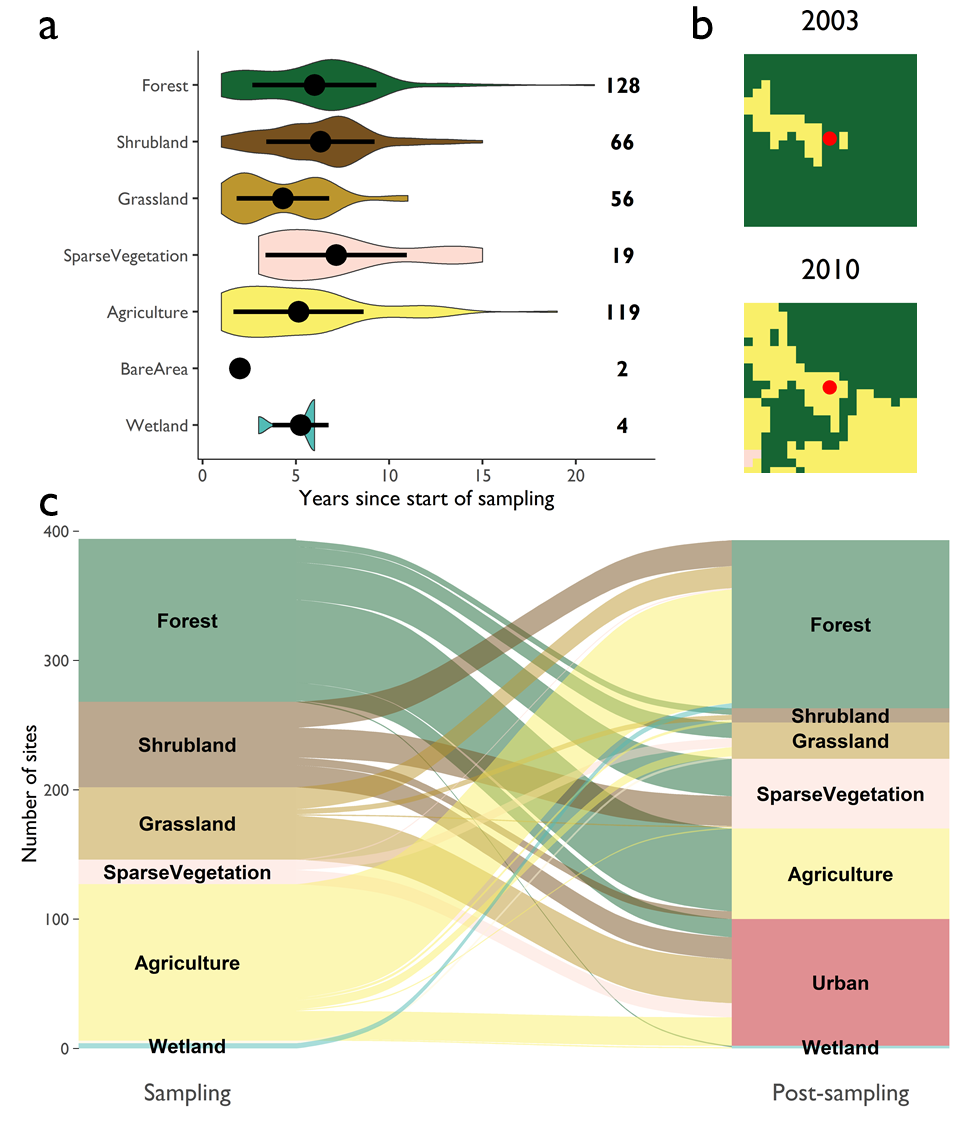
\includegraphics[width=.8\textwidth]{chapter6/F01}
\caption{ Remote sensing data can help identify areas suitable for resampling of local biodiversity. Combining sites from the PREDICTS project (Chapter \ref{C02}-\ref{C04}) and time series of land cover \citep{ESA2017}, I assessed whether land cover has changed after biodiversity sampling (\textbf{a}) PREDICTS sites (394 sites, 115 studies) with a land-cover change after biodiversity had been sampled (average 5.57 $\pm$ 3.3 SD years) according to the ESA LC product \citep{ESA2017}. Colours and y-axis indicate the land cover at the time of biodiversity sampling. The x-axis shows the years the site remained in a given land cover (mean estimate and standard deviation shown as dots and error bars) before a land-cover change occurred. Numbers show the total number of sites. (\textbf{b}) Example of a PREDICTS site which was forest-covered at the time of biodiversity sampling in 2003 but was converted to agriculture seven years later. (\textbf{c}) Flow diagram showing the land-cover sequences observed for sites with a post-sampling land-cover change.}
\label{F06_01}
\end{figure}
% -------------------------------------------- %

To infer how land change impacts local biodiversity, specific sampling designs are necessary \citep{DePalma2018}. The best way of assessing the impacts of land change on biodiversity are before-after-control-impact (BACI) study designs \citep{Cardinale2018,DePalma2018}. Such data could quantify the immediate difference in local biodiversity after land change \citep{Ratajczak2018}, taking attributes of land change \citep{Watson2014}, site-specific local factors \citep{Jung2016} and variability among species assemblages \citep{Dornelas2013,Franca2016} into account. However, such BACI data are currently not readily available. A new phase of the PREDICTS project (labelled PREDICTS-2) aims to systematically collect estimates of local biodiversity before and after land change. Remote sensing data \textendash\ either using a land change detection algorithm (Chapter \ref{C03}) or readily available land cover products (Chapter \ref{C04}) \textendash\ can help to identify sites where land cover has or has not changed after local biodiversity sampling (Figure \ref{F06_01}). There is an opportunity to sample those sites again \textendash\ preferably using identical methods and observers \textendash\ to obtain BACI estimates of local biodiversity in response to land change \citep{DePalma2018}. Such data would further improve our understanding of the impacts of land change on local biodiversity.

\subsection{Improving availability of remotely-sensed estimates of land change}
\label{C06_0304}

The availability and accessibility of remote sensing data continues to improve. The move of the global Landsat archive into the public domain in 2008 enabled unprecedented and free access to satellite imagery \citep{Wulder2015}. Opposed to the early 1990s and 2000s, when mostly only single satellite images were analysed in a time-consuming process, modern satellite-based remote sensing analyses increasingly utilize entire time series of satellite imagery \citep{Kennedy2014,Hermosilla2015a}. The development of new land change detection \citep{Coppin2004,Abercrombie2016,Zhu2017} and machine learning algorithms \citep{Maxwell2018}, and the rise of cloud processing environments \citep{Gorelick2017} have further supported the creation of temporally consistent remotely-sensed land cover products globally \citep{ESA2017,Hermosilla2018,Sulla-Menashe2019}. These developments have led some to declare that a new area of land cover analysis has emerged, fittingly called as “Land cover 2.0” \citep{Wulder2018}. It is highly likely that future investigations into the impacts of land change on local biodiversity can rely on improved data and algorithm availability.

There are a number of promising avenues for future research linking biodiversity and remotely-sensed land change data: More efforts are needed to (\textit{i}) create and utilize remotely-sensed proxies of land-use change globally, piloted for instance for cropland size \citep{Fritz2015} and yield \citep{Lobell2015}, pasture grazing intensity \citep{Rufin2015,Aguiar2017} or forest plantation rotations \citep{LeMaire2014}; (\textit{ii}) clearly determine natural and anthropogenic drivers of land change, as has recently been done for forests globally \citep{Curtis2018}, (\textit{iii}) consider additional data to extend the available time period \textendash\ such as air borne historical photographs \citep{SZABO2011,Cousins2015} or “legacy” satellite imagery predating the 1980s (\eg Landsat 1-3, Figure \ref{F01_01}), which were not readily available at the time this thesis was conducted.

\section{Concluding remarks}
\label{C06_04}

The impacts of land change on local biodiversity are complex and require looking beyond present differences in land use and/or land cover. Frameworks such as the one developed by \cite{Watson2014} are useful to incorporate dynamics of land change into global biodiversity models. The results presented here demonstrate that attributes of past land change impact local biodiversity differently on a global scale and show how remote sensing can be used to quantify spatio-temporal land change. Overall these results show how new insights into local biodiversity patterns can be gained by combining existing data sources.

We live in an age of unprecedented availability of data. This situation provides new opportunities to detect and quantify links between remotely sensed land change and biodiversity data. These opportunities could lead to improved and ultimately near real-time predictions of biodiversity change following land change. However, while technology and data-driven research may assist in providing further evidence and understanding of environmental issues, the preservation of biodiversity is ultimately up to government interventions and societal actions. I hope that quantitative evidence \textendash\ based on data syntheses such as those presented in this thesis \textendash\ will support decision making and that the results of this thesis contribute towards this goal.    


\clearpage
%\bibliography{content/04Chapter}

%\appendix
%\begingroup
%  % SI - Figure 1 Missing data
\begin{figure}[h]
\centering
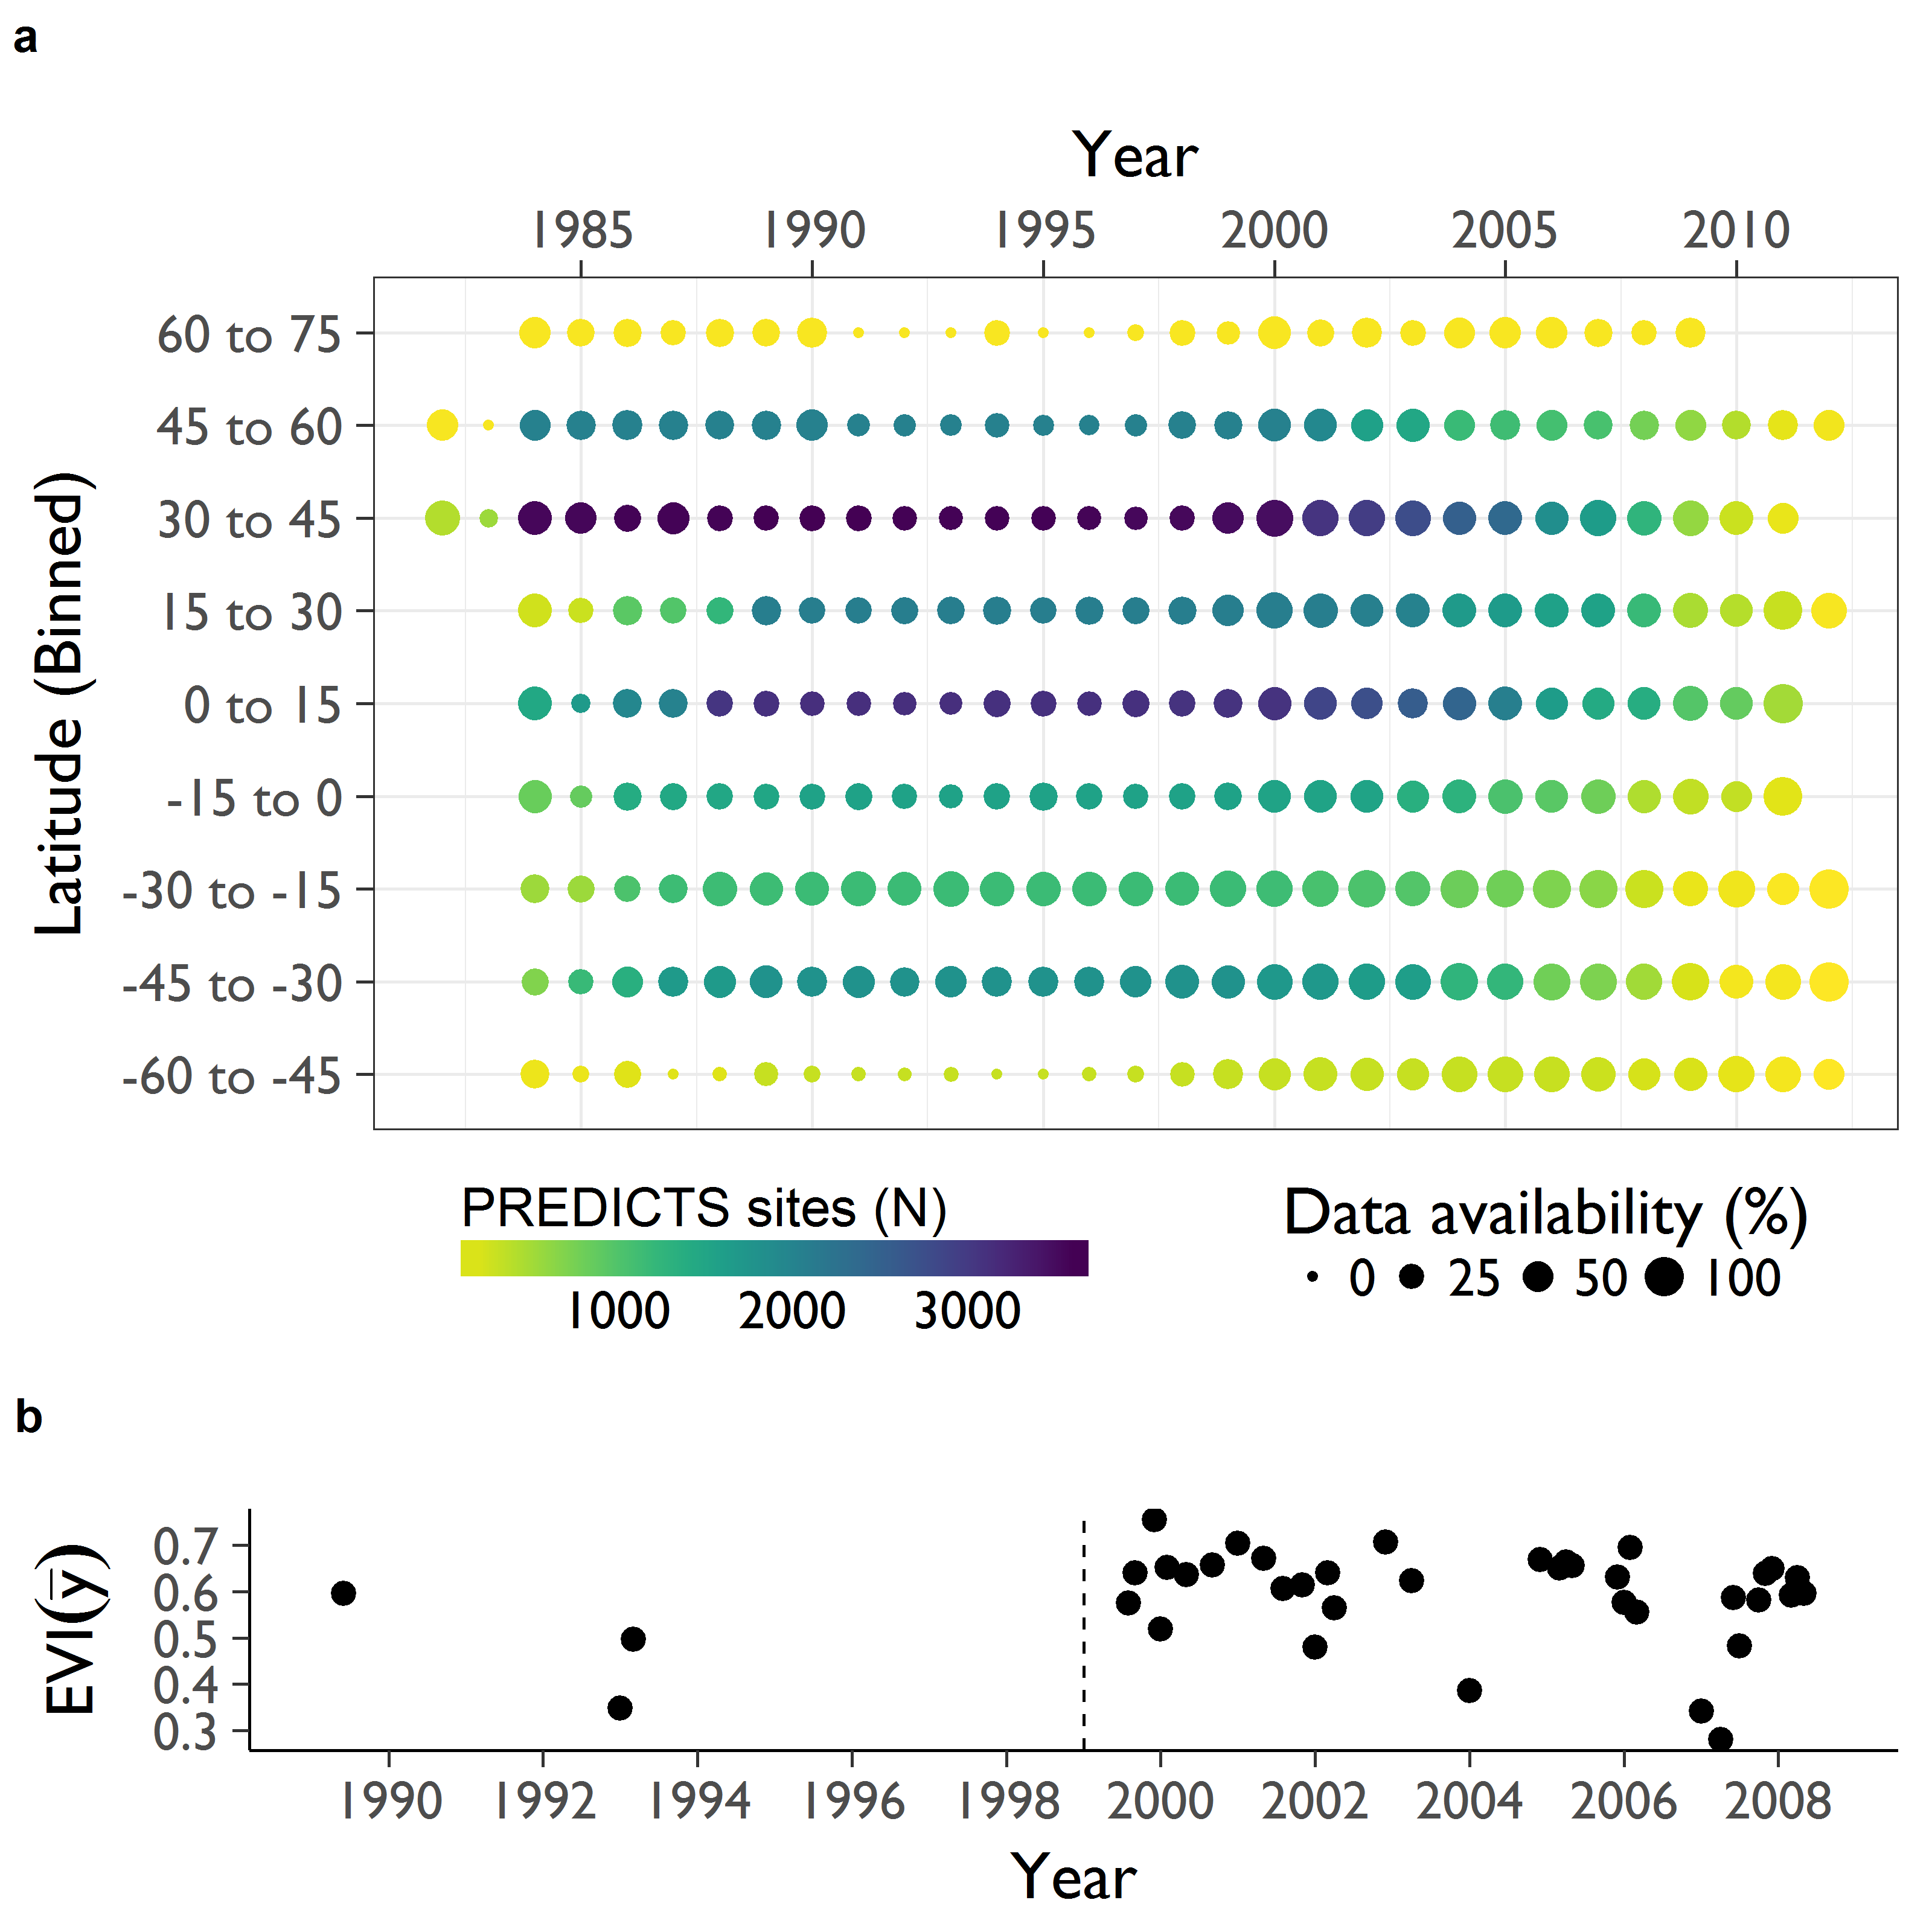
\includegraphics[width=1\textwidth]{chapter3/SI01}
\caption{ Average temporal distribution of Landsat data and an example times series of Landsat data. (\textbf{a}) Distribution of available Enhanced Vegetation Index (EVI) data in years covered by the Landsat missions. Points show the average monthly EVI data availability per year (0 to 12 months of data) across time series and PREDICTS sites grouped by 15\textdegree latitude bins. The size of points indicates the mean data availability (0 to 100\% with 100\% having 12 months of available data in a given year), while the colour shows the number of PREDICTS sites contributing to the mean (as PREDICTS sites were sampled in varying years). (\textbf{b}) Example time series for one PREDICTS site with a high proportion of missing data before 1999. In all analyses such time series were truncated to the period from 1999 onwards (indicated by the dashed line).}
\label{SI03_01}
\end{figure}

% SI - Figure 2 Binning
\begin{figure}[h]
\centering
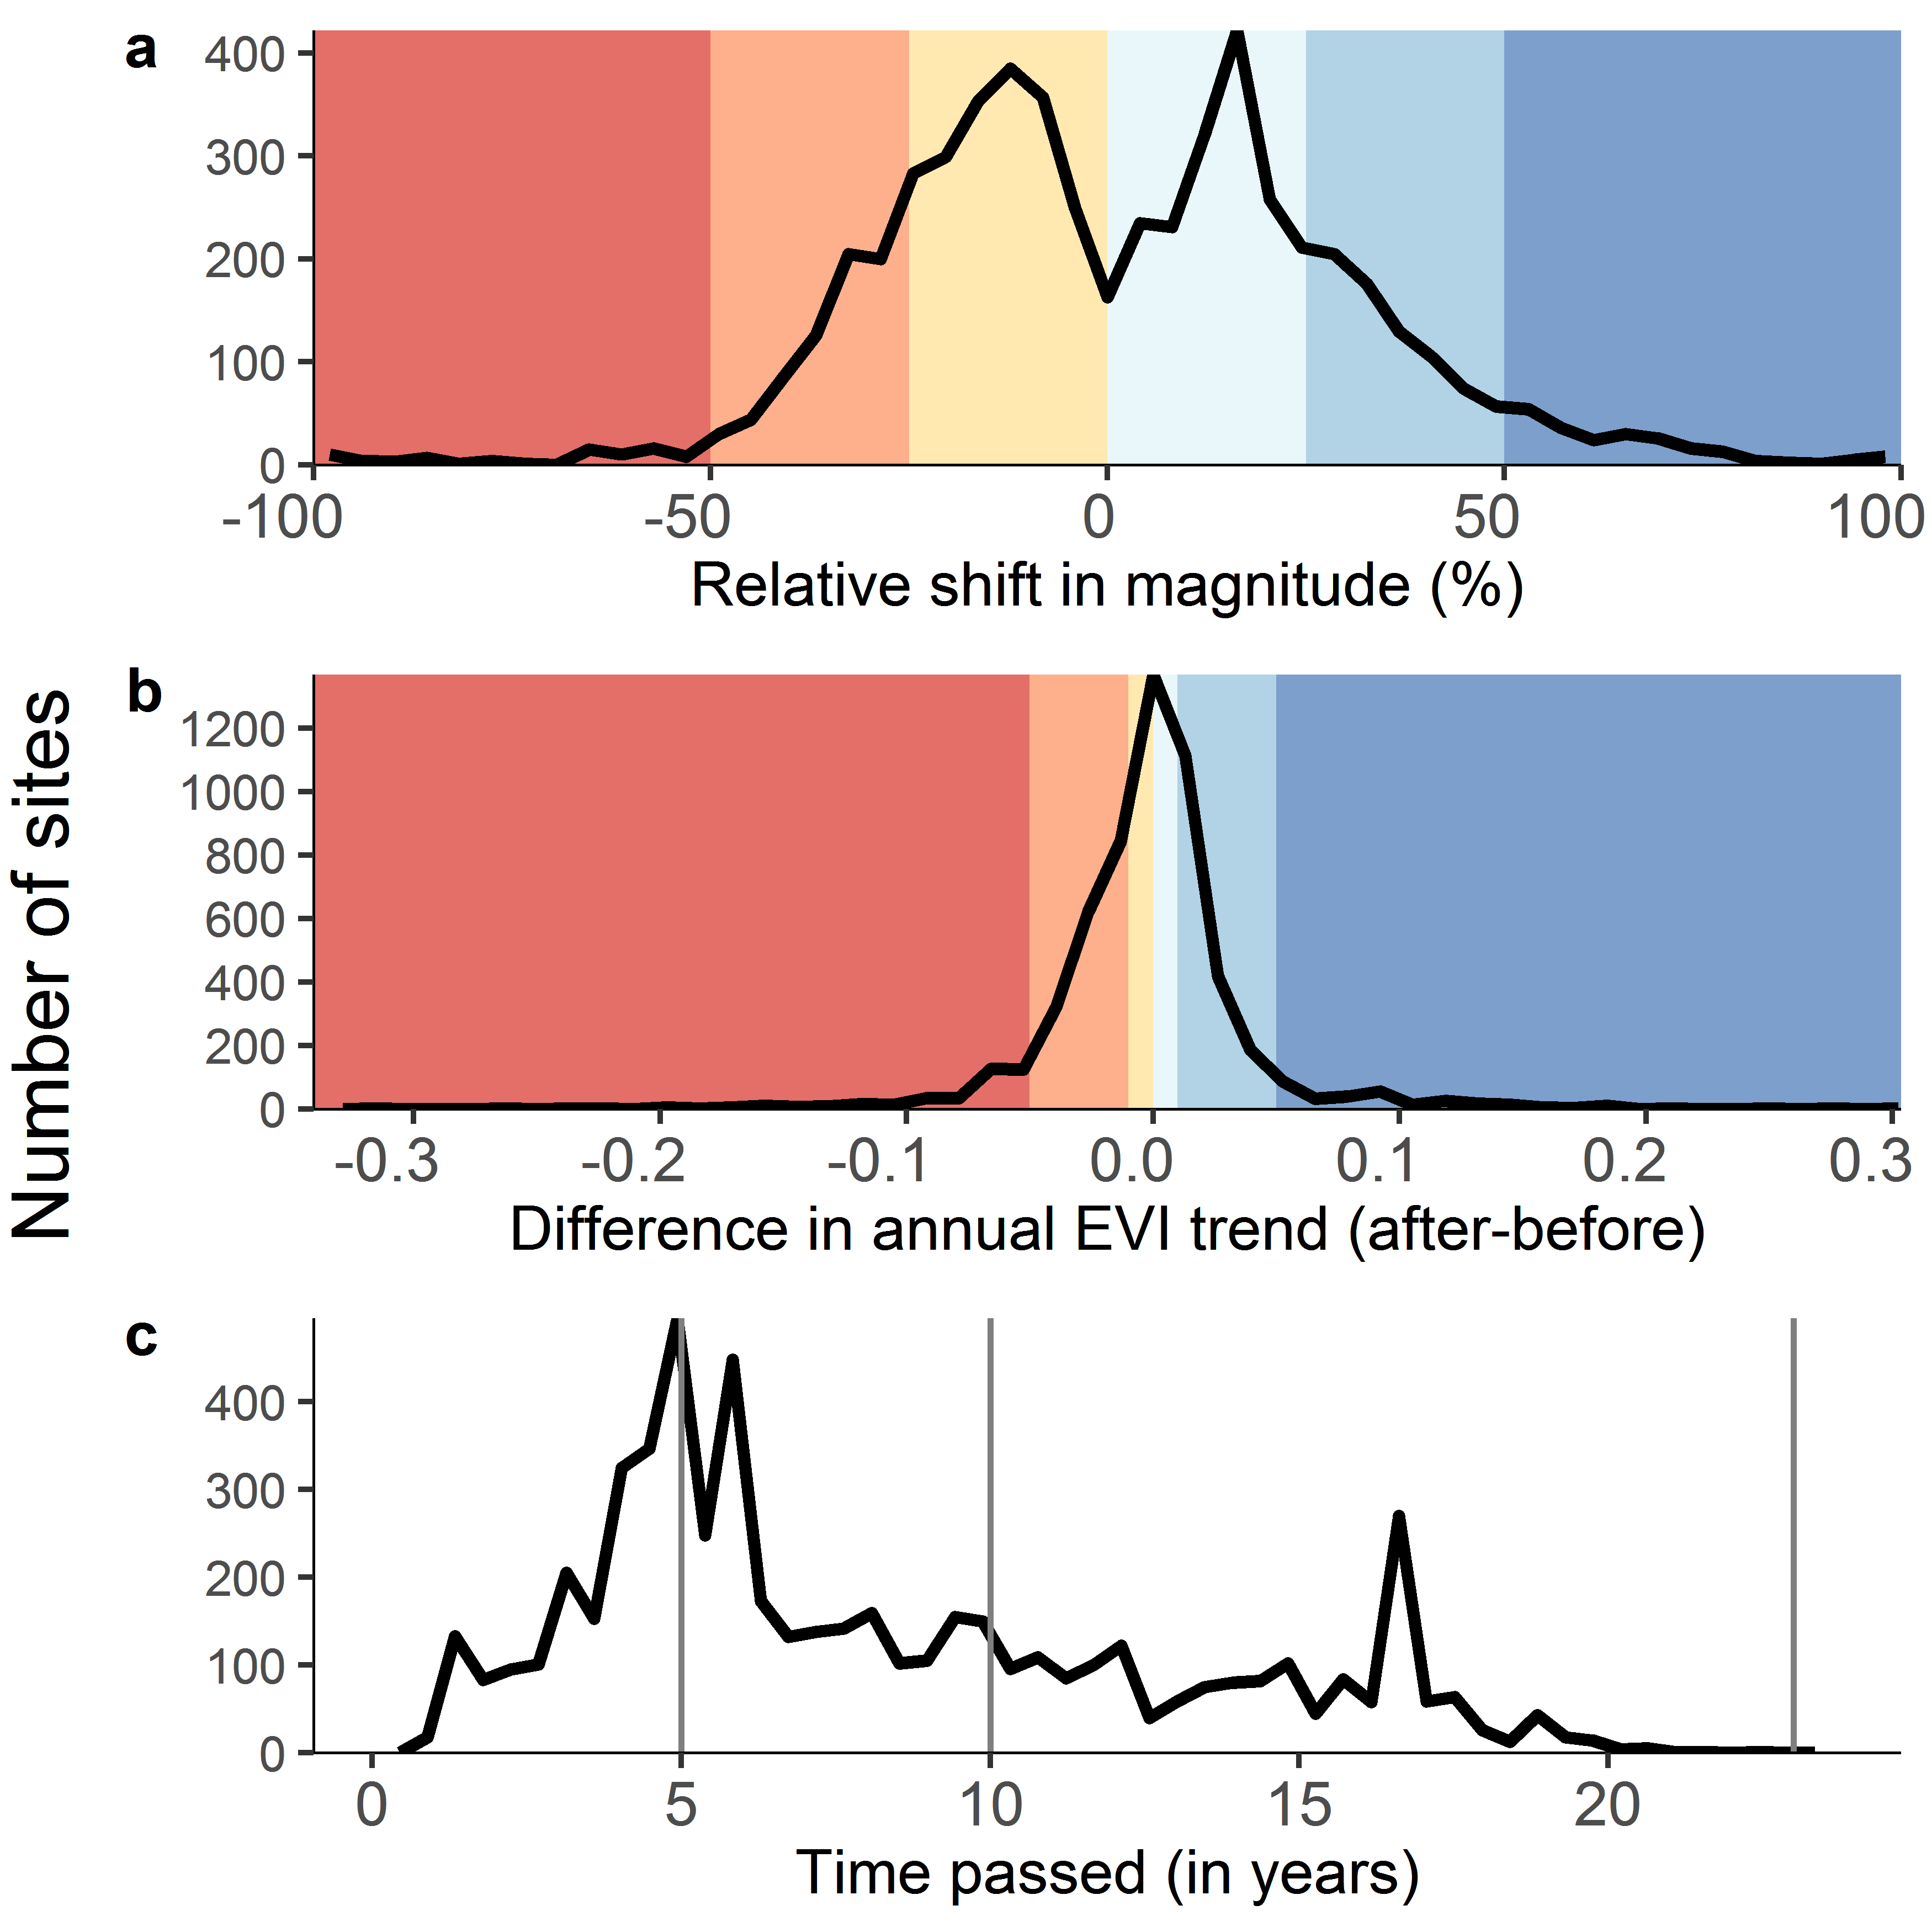
\includegraphics[width=1\textwidth]{chapter3/SI02}
\caption{ Number of sites with abrupt land change per attribute. Number of sites (black line) per attribute of abrupt land change with (\textbf{a}) the relative shift in magnitude, (\textbf{b}) the shift in trend as difference in annual EVI trend, and (\textbf{c}) the time passed between abrupt land change and biodiversity sampling. Background colours in (\textbf{a}) and (\textbf{b}) indicate the binning into six groups for shifts in magnitude (> 50\%, > 25\% to $\leq$ 50\%, and $\leq$ 25\% EVI loss [$---$ to $-$] or gain [$+++$ to $+$]), and in trend (0.01, 0.05, and > 0.05 annual negative [$---$ to $-$] to positive [$+++$ to $+$] EVI trend differences). Gray lines in (\textbf{c}) delineate bins of time passed ($\leq$ 5 years, > 5 and $\leq$ 10 years, and >10 years). Colours as in Figure \ref{F03_02}.}
\label{SI03_02}
\end{figure}

% SI Table 1------ %
% From here https://www.tablesgenerator.com/
\begin{table}[]
\centering
\caption{Number of PREDICTS sites and studies with an abrupt land change. Shown as either a change in magnitude (columns) and/or change in trend (trend). Symbols as in Figure \ref{F03_02}. }
\label{SIT03_01}
\begin{tabular}{@{}lllllllllll@{}}
                                          &                                           & \multicolumn{7}{c}{\textbf{Shift in magnitude}}                                                                                                                                                                    &                               &                             \\
                                          &                                           & \textbf{- - -}             & \textbf{- -}                & \textbf{-}                   & \textbf{0}                    & \textbf{+}                   & \textbf{+ +}                & \textbf{+ + +}              & \textbf{Total sites}          & \textbf{Studies}            \\ \cmidrule(l){3-11} 
                                          & \multicolumn{1}{l|}{- - -}                & 2                          & 8                           & 192                          & NA                            & 73                           & 26                          & 22                          & \cellcolor[HTML]{EFEFEF}323   & \cellcolor[HTML]{C0C0C0}57  \\
                                          & \multicolumn{1}{l|}{- -}                  & 7                          & 281                         & 642                          & NA                            & 497                          & 158                         & 53                          & \cellcolor[HTML]{EFEFEF}1638  & \cellcolor[HTML]{C0C0C0}175 \\
                                          & \multicolumn{1}{l|}{-}                    & 7                          & 88                          & 256                          & NA                            & 231                          & 154                         & 53                          & \cellcolor[HTML]{EFEFEF}789   & \cellcolor[HTML]{C0C0C0}184 \\
                                          & \multicolumn{1}{l|}{0}                    & NA                         & NA                          & NA                           & 10102                         & NA                           & NA                          & NA                          & \cellcolor[HTML]{EFEFEF}10102 & \cellcolor[HTML]{C0C0C0}358 \\
                                          & \multicolumn{1}{l|}{+}                    & 9                          & 102                         & 399                          & NA                            & 410                          & 205                         & 49                          & \cellcolor[HTML]{EFEFEF}1174  & \cellcolor[HTML]{C0C0C0}237 \\
                                          & \multicolumn{1}{l|}{\textbf{+ +}}         & 47                         & 172                         & 342                          & NA                            & 465                          & 254                         & 86                          & \cellcolor[HTML]{EFEFEF}1366  & \cellcolor[HTML]{C0C0C0}224 \\
\multirow{-7}{*}{\textbf{\rotatebox{90}{Shift in trend}}} & \multicolumn{1}{l|}{\textbf{+ + +}}       & 12                         & 137                         & 47                           & NA                            & 34                           & 12                          & 31                          & \cellcolor[HTML]{EFEFEF}273   & \cellcolor[HTML]{C0C0C0}56  \\
                                          & \multicolumn{1}{l|}{\textbf{Total sites}} & \cellcolor[HTML]{EFEFEF}84 & \cellcolor[HTML]{EFEFEF}788 & \cellcolor[HTML]{EFEFEF}1878 & \cellcolor[HTML]{EFEFEF}10102 & \cellcolor[HTML]{EFEFEF}1710 & \cellcolor[HTML]{EFEFEF}809 & \cellcolor[HTML]{EFEFEF}294 &                               &                             \\
                                          & \multicolumn{1}{c|}{\textbf{Studies}}     & \cellcolor[HTML]{C0C0C0}34 & \cellcolor[HTML]{C0C0C0}135 & \cellcolor[HTML]{C0C0C0}246  & \cellcolor[HTML]{C0C0C0}358   & \cellcolor[HTML]{C0C0C0}263  & \cellcolor[HTML]{C0C0C0}171 & \cellcolor[HTML]{C0C0C0}83  &                               &                            
\end{tabular}
\end{table}
% ------ %

% SI - Figure 3 Cross-correlations
\begin{figure}[h]
\centering
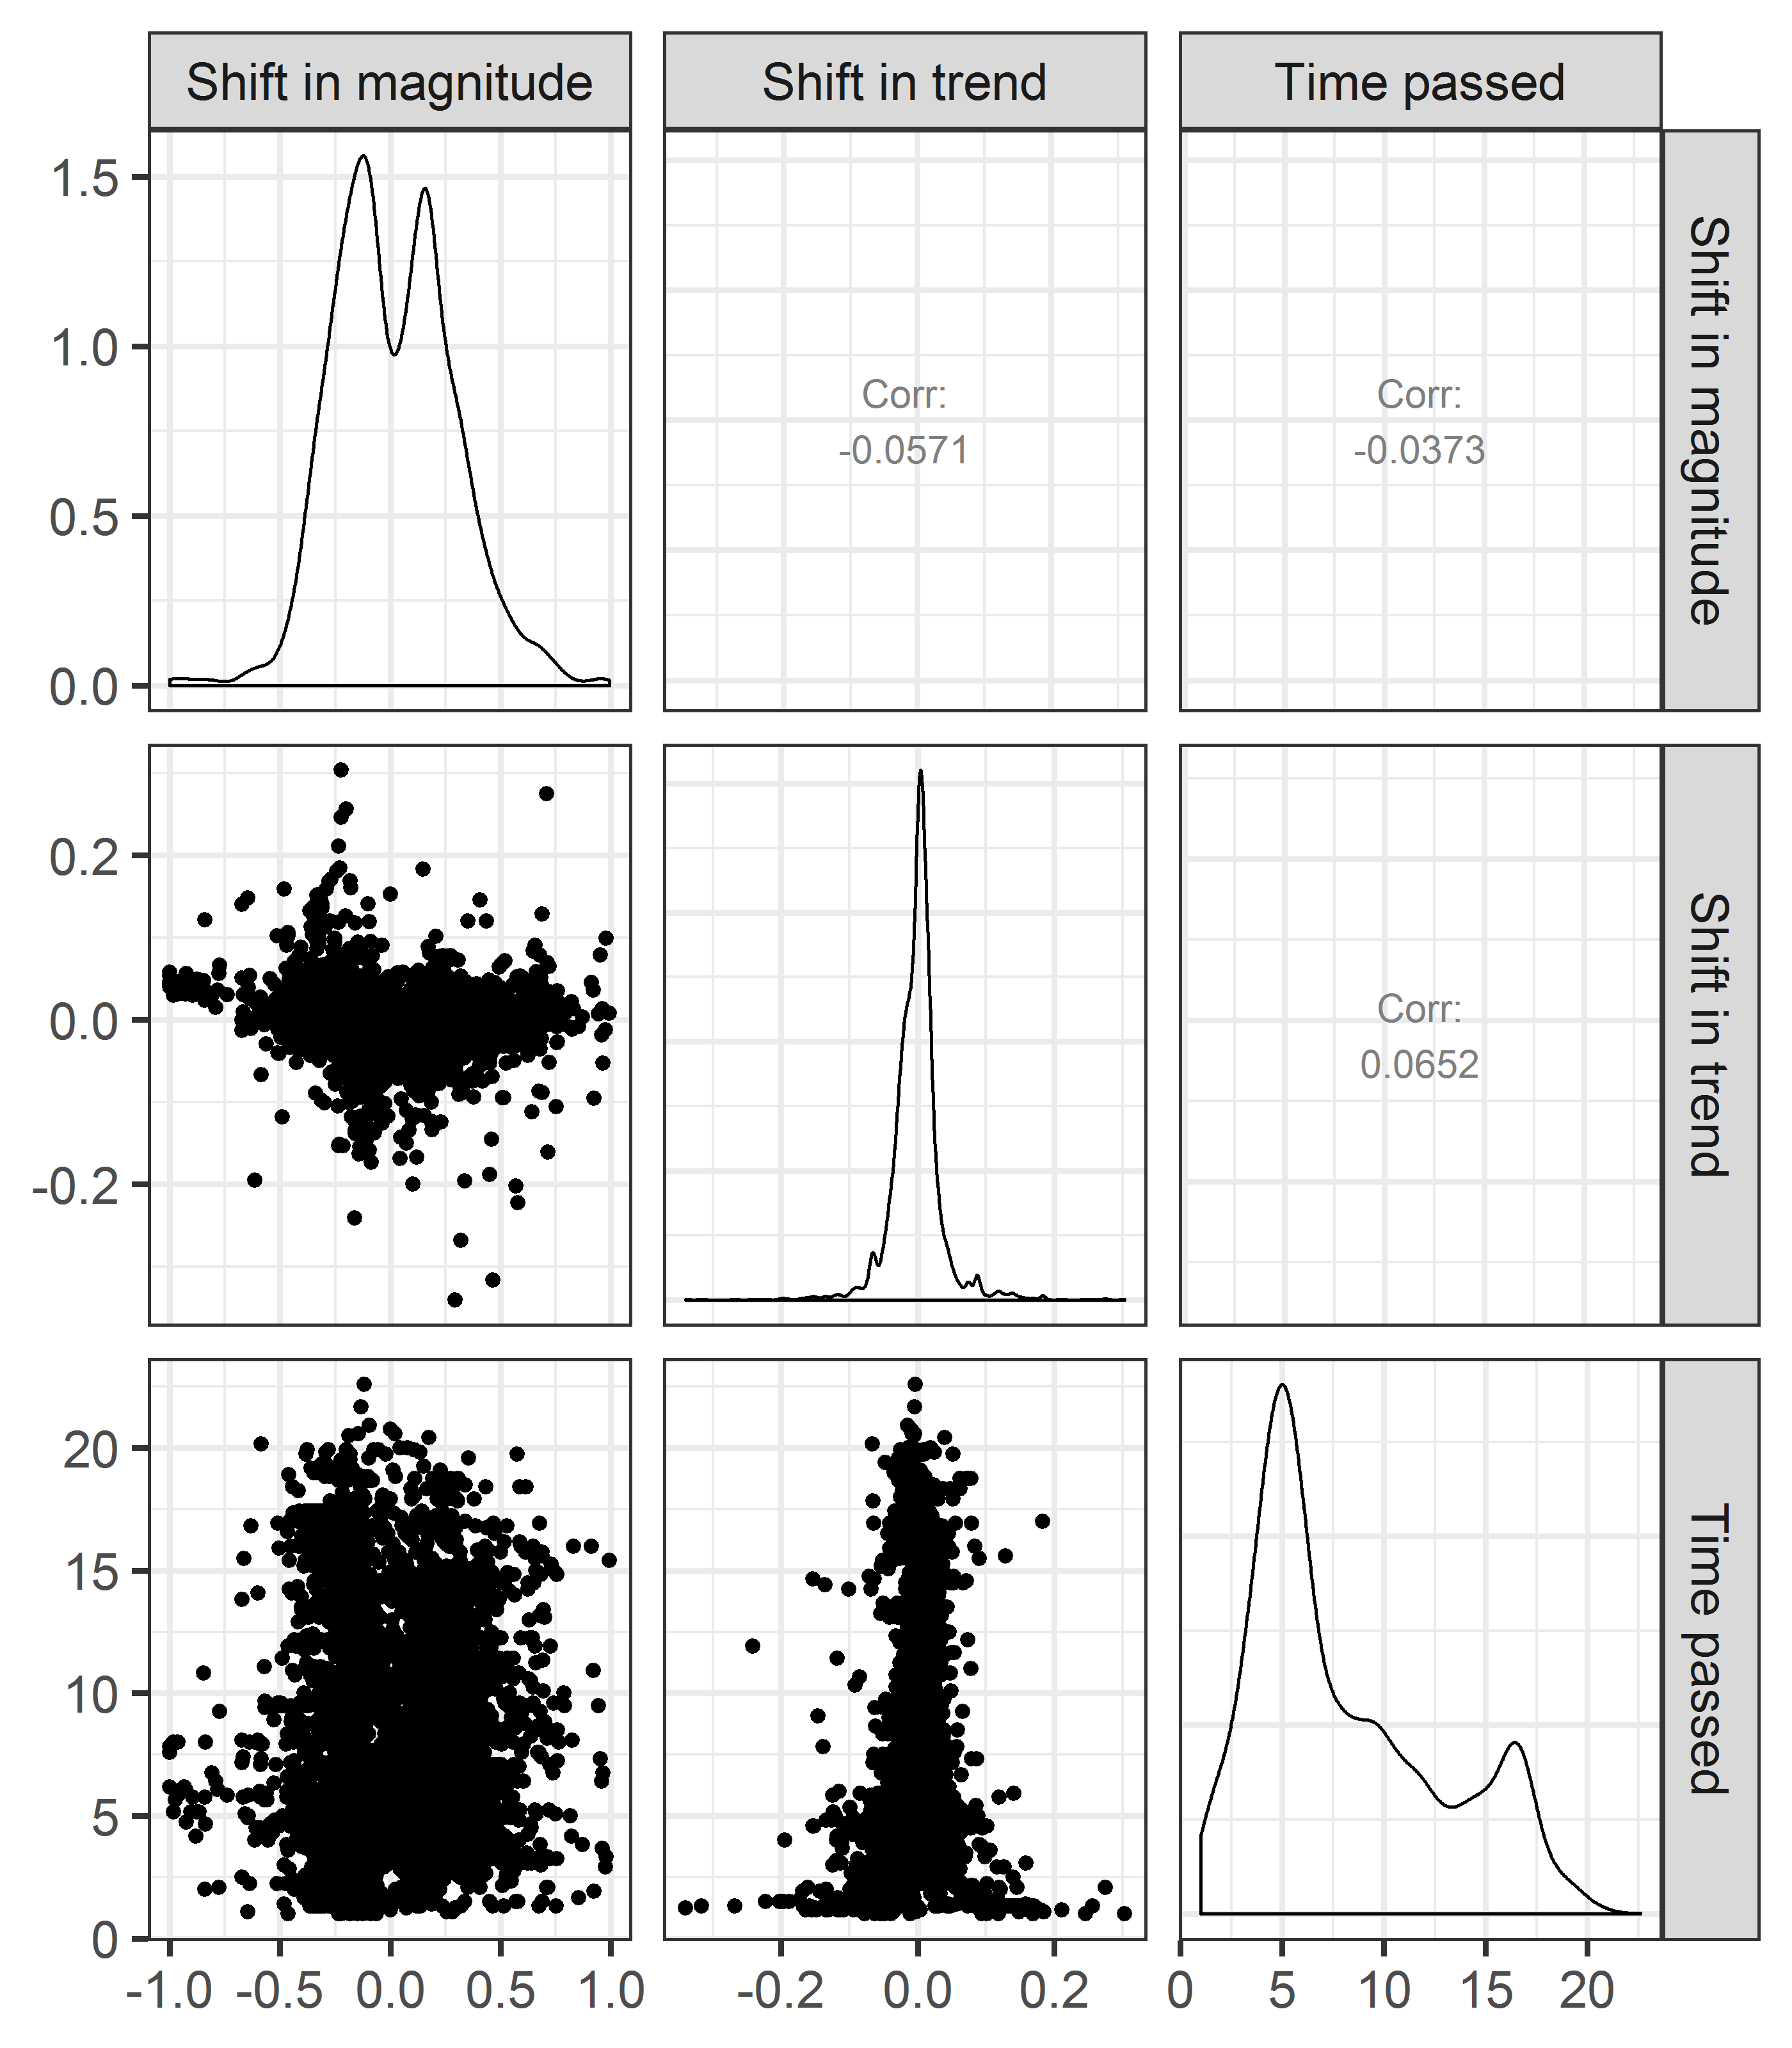
\includegraphics[width=1\textwidth]{chapter3/SI03}
\caption{ Correlations between attributes of abrupt land change. Showing shifts in magnitude, trend and time passed (see Methods). The lower facets show a point density plot, the upper facets the Pearson correlation coefficient between pairs of attributes and the diagonal a density plot.}
\label{SI03_03}
\end{figure}

%\endgroup
 %Synthesis
\endgroup

%\input{front/Acronyms.tex}

%---------------------------------------------------
% BIBLIOGRAPHY
%---------------------------------------------------
\backmatter
\clearpage
\phantomsection
\bibliography{content/allreferences}
%\clearpage\pagestyle{empty}
\pdfbookmark[0]{Colophon}{colophon}
\hfill

\vfill

\begin{flushright}
Lorem ipsum dolor sit amet, consectetur adipiscing elit. Integer nec venenatis augue. Maecenas sed egestas elit, quis ultrices lacus. Maecenas hendrerit massa nisi, congue congue quam pretium eu. Proin erat quam, iaculis ac iaculis nec, rhoncus vitae tortor. Pellentesque neque eros, aliquet tincidunt enim sed, volutpat ultrices nibh. Nullam feugiat gravida velit, ut aliquam est finibus ac. Cras pharetra nibh enim, vel lacinia enim pulvinar eget. Maecenas gravida ante vitae convallis eleifend. 
\end{flushright} 


%---------------------------------------------------
% APPENDICES
%---------------------------------------------------
\appendix
\counterwithin{figure}{section}
\counterwithin{table}{section}
\chapter{Appendix}
\begingroup
  \section{Appendix - Chapter 2}
  % SI - Figure 1 Flowchart
\begin{figure}[htb]
\centering
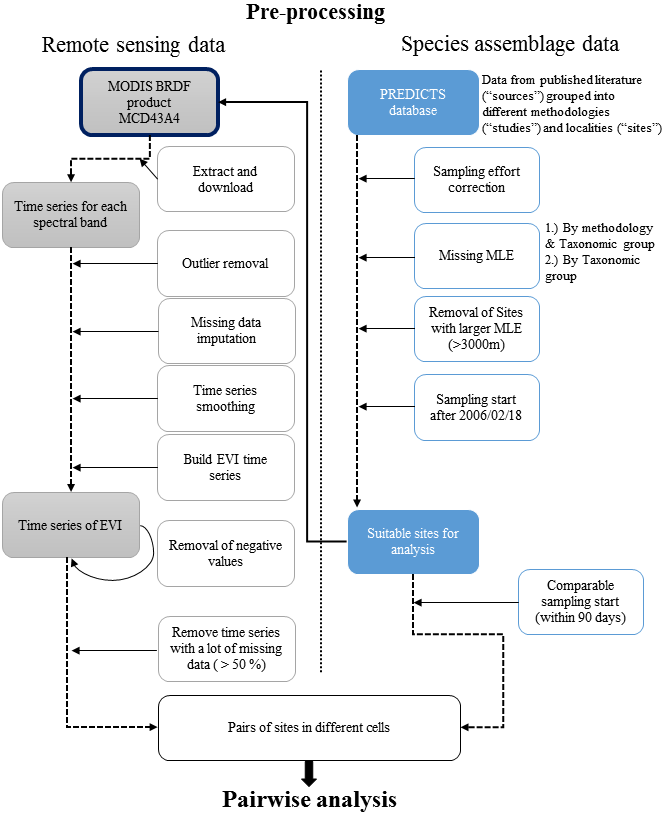
\includegraphics[width=1\textwidth]{chapter2/SI01}
\caption{ Flow chart showing all pre-processing steps of the analysis for both remote sensing and species assemblage data. Remote sensing data were derived from the MODIS Bidirectional reflectance distribution function (BRDF) MCD43A4 product (\href{https://tinyurl.com/mcd43a4-v006}{https://tinyurl.com/mcd43a4-v006}) and time series of the Enhanced Vegetation Index (EVI) were calculated for the analysis (see methods \ref{C02_02}). Species assemblage data originates from the Projecting Responses of Ecological Diversity In Changing Terrestrial Systems project (PREDICTS, \href{http://www.predicts.org.uk/}{http://www.predicts.org.uk/}). MLE stands for the Maximum Linear Extent as defined by \citep{Hudson2016}.}
\label{SI02_01}
\end{figure}

% SI - Figure 2 Flowchart
\begin{figure}[htb]
\centering
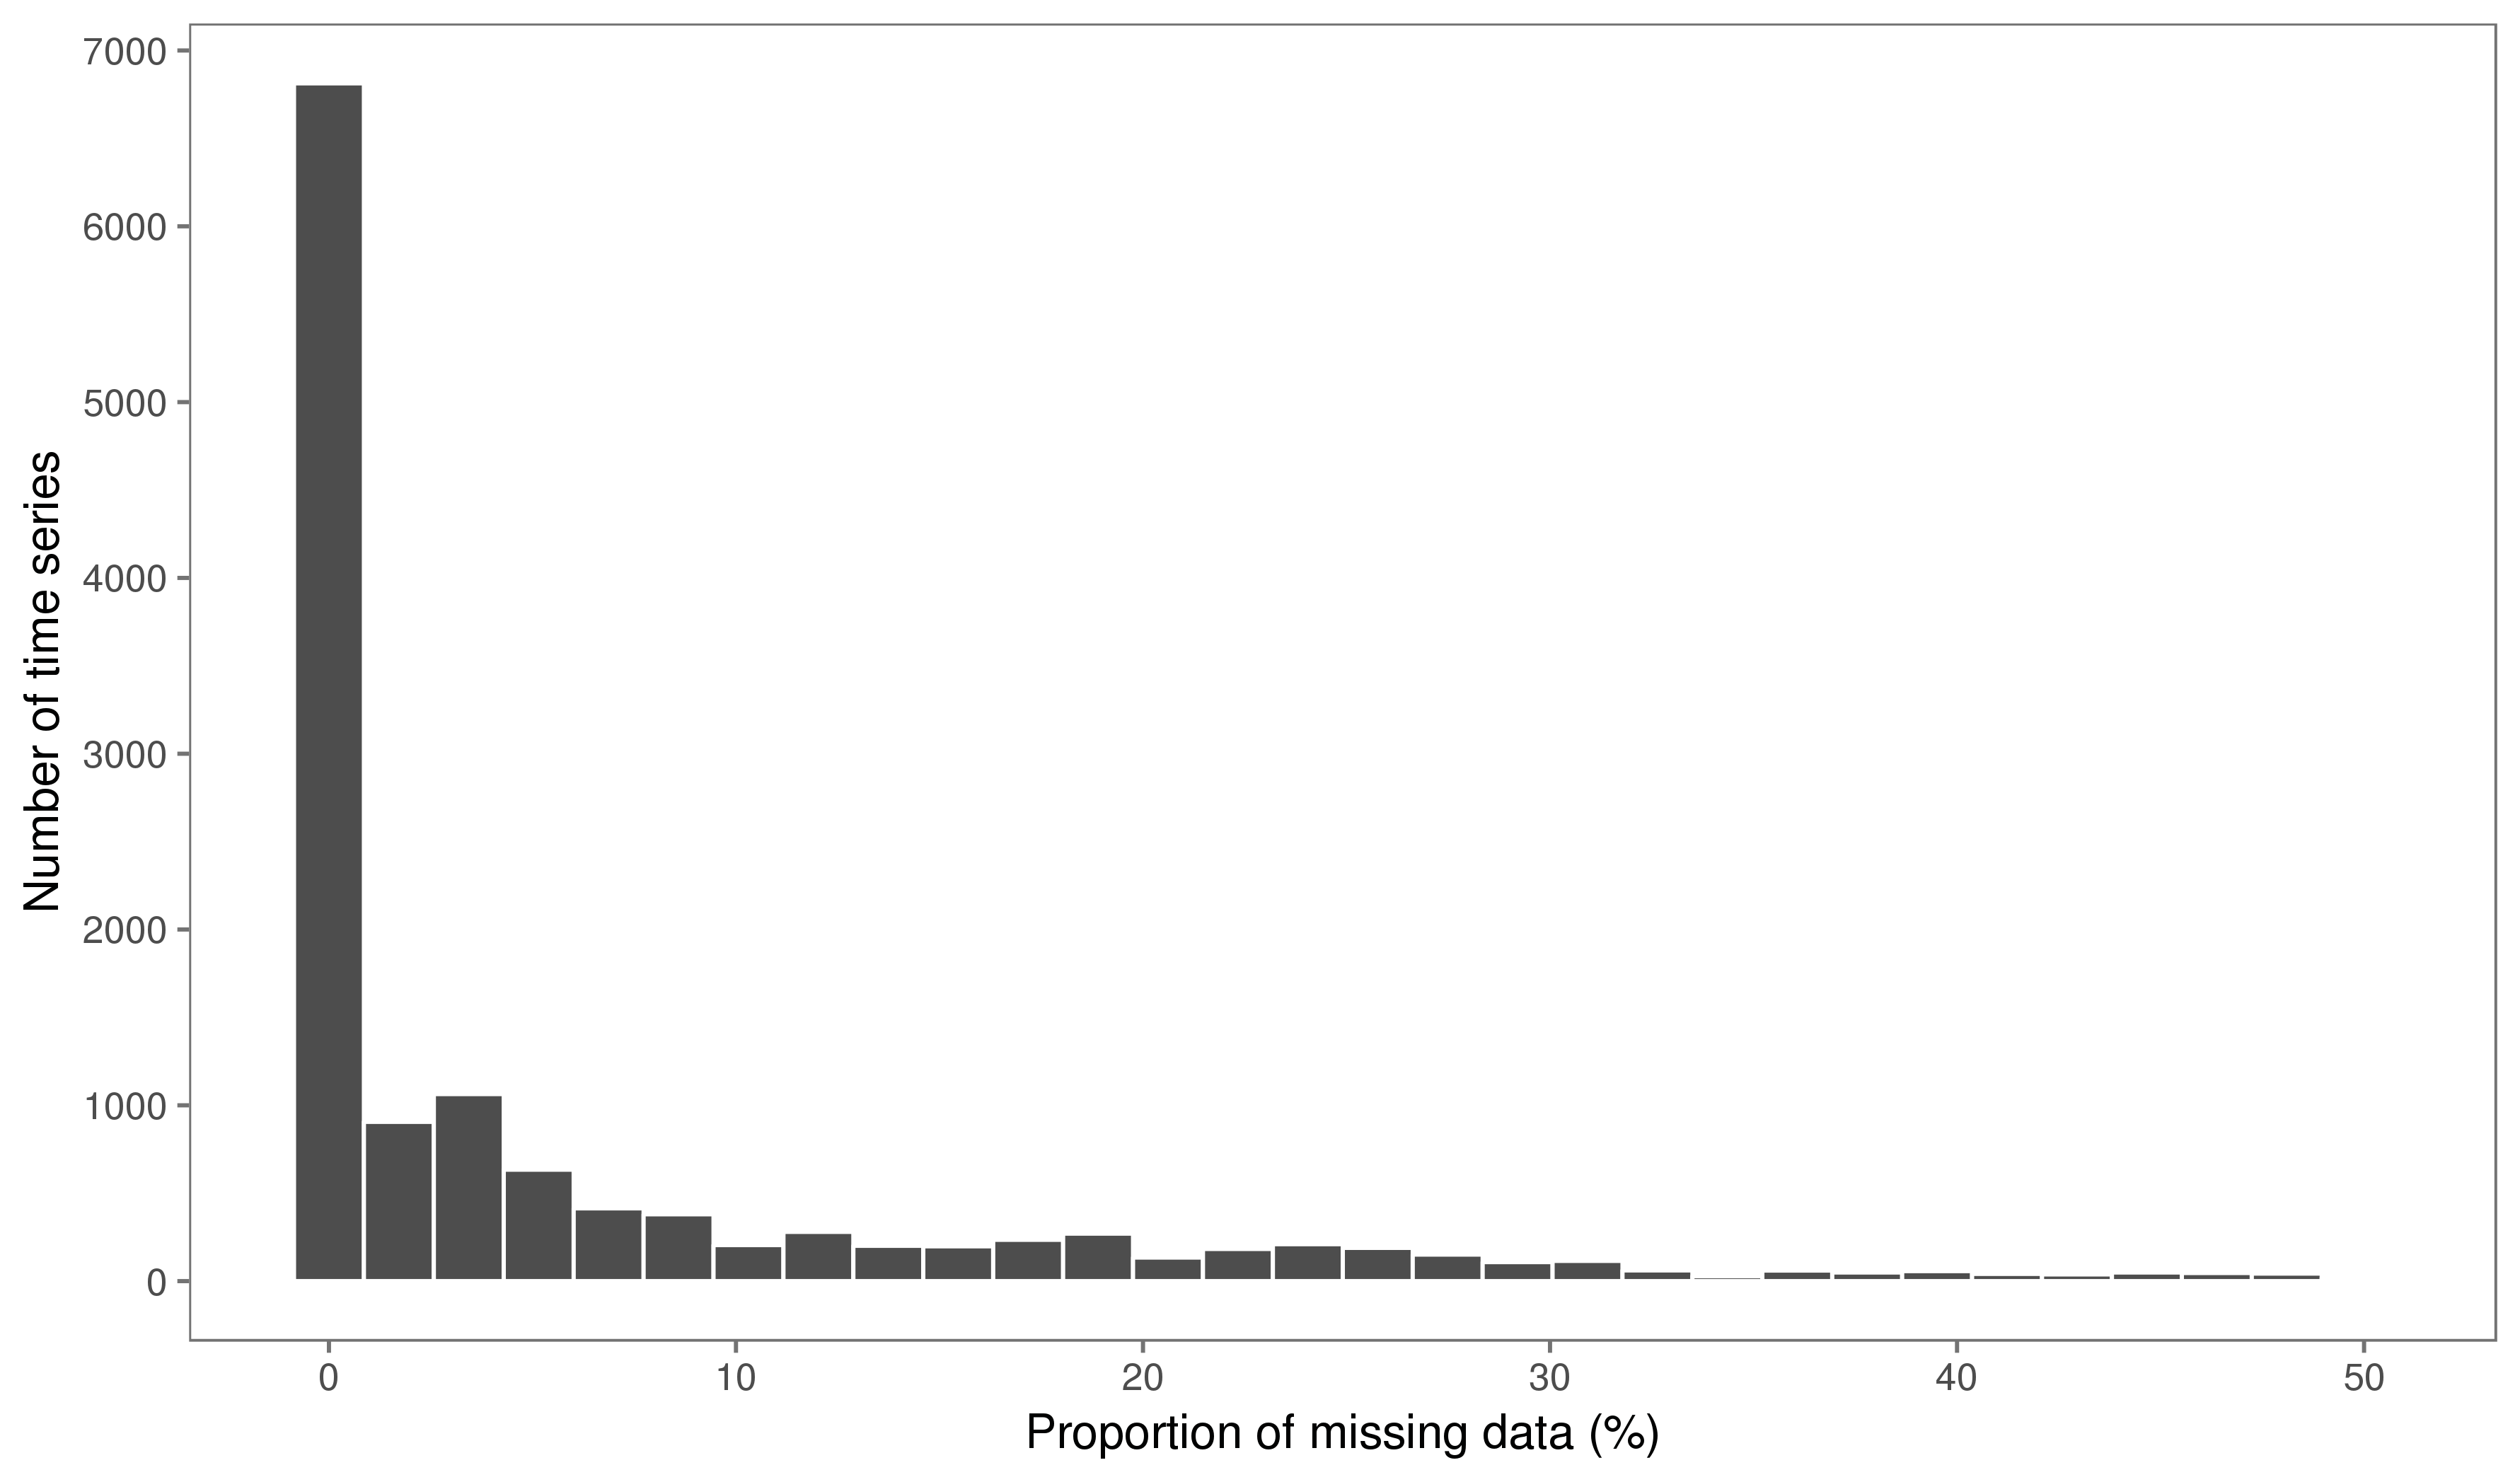
\includegraphics[width=1\textwidth]{chapter2/SI02}
\caption{ Distribution of proportion of missing data (not interpolated) across all time series used. }
\label{SI02_02}
\end{figure}

% SI - Figure 3 Pairwise permutation procedure
\begin{figure}[htb]
\centering
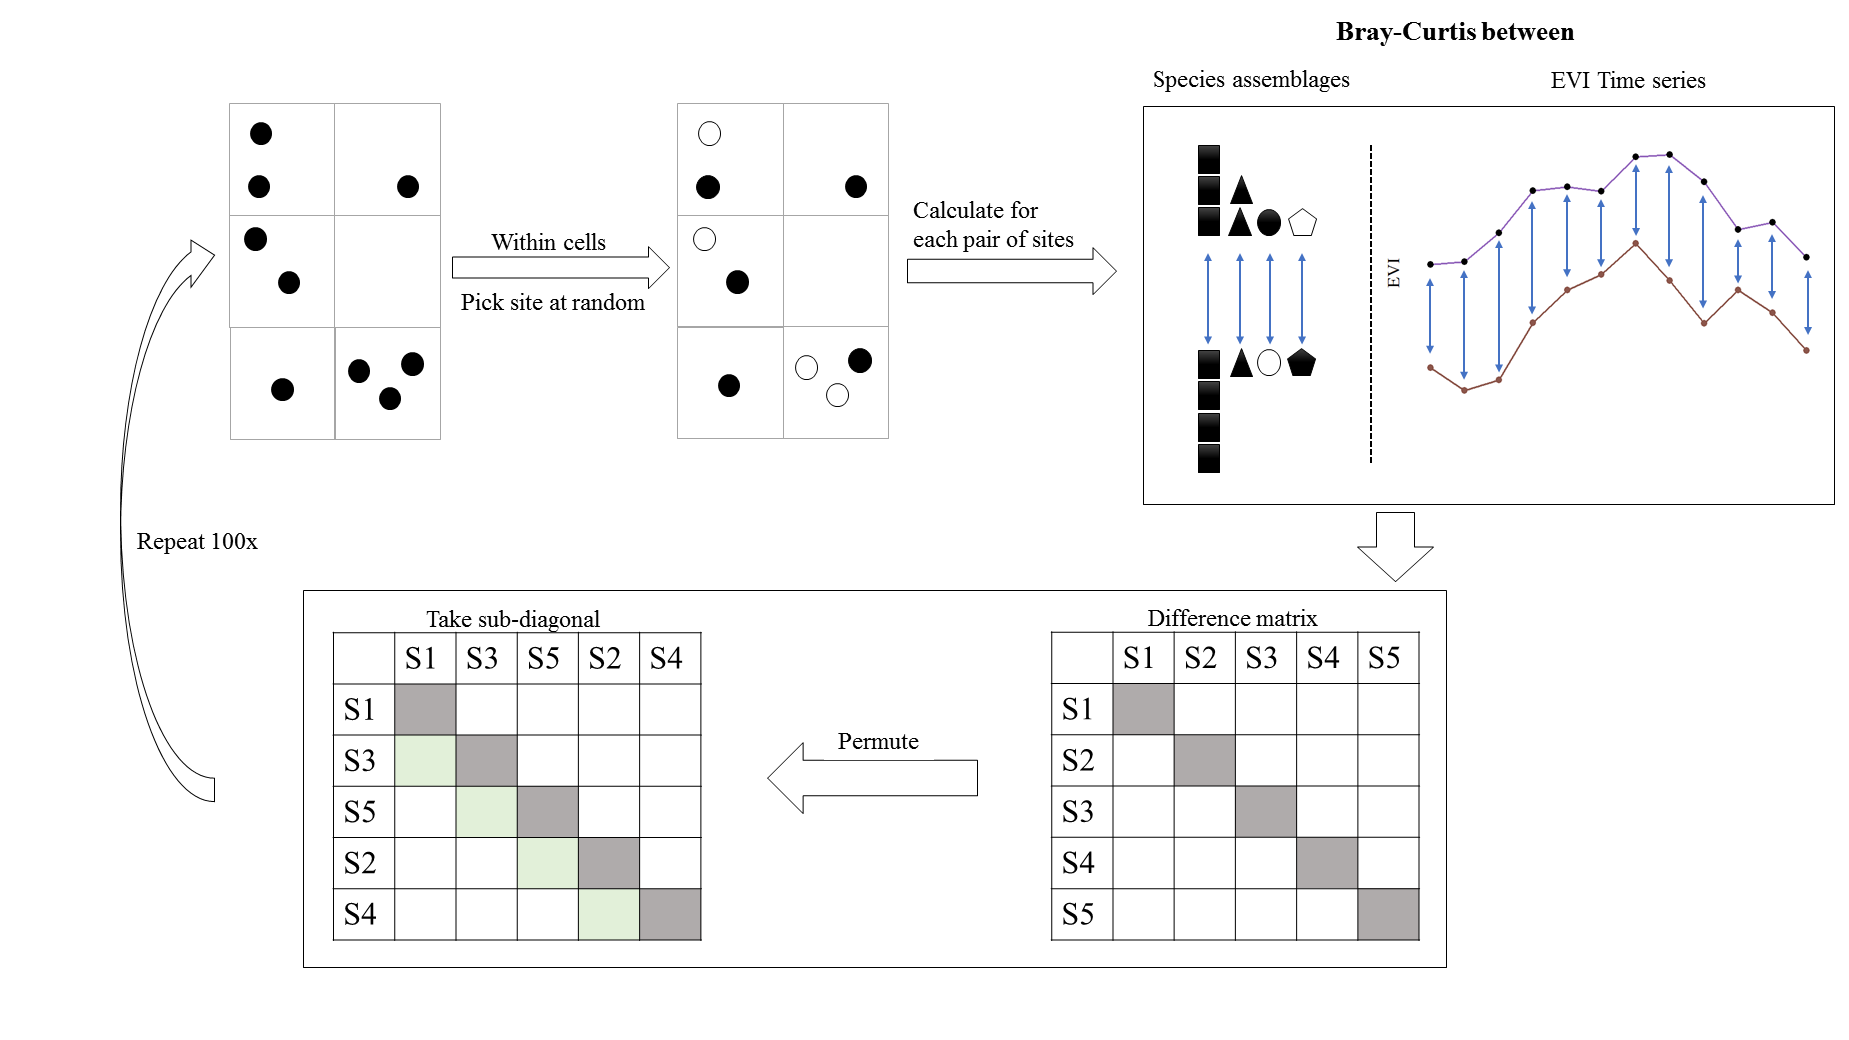
\includegraphics[width=1\textwidth]{chapter2/SI03}
\caption{ Diagram of how the permutations of mutually independent pairwise comparisons were generated. Black dots represent 9 theoretical sites of a study within MODIS grid cells of which one site (S1 – S5) per grid cell was randomly selected. We then calculated two dissimilarity matrices one matrix for the dissimilarity between species assemblages in that grid cell and all other grid cells within the study, and the other matrix for the dissimilarity between time series of the EVI of these grid cells.  For the time series, the Bray-Curtis index was calculated between the EVI values at each time step. For both species assemblages (symbols of varying number and shape) and EVI time series, the obtained dissimilarity matrix was permuted and the sub-diagonal taken for subsequent analysis. }
\label{SI02_03}
\end{figure}

% SI - Figure 4 Pairwise permutation procedure
\begin{figure}[htb]
\centering
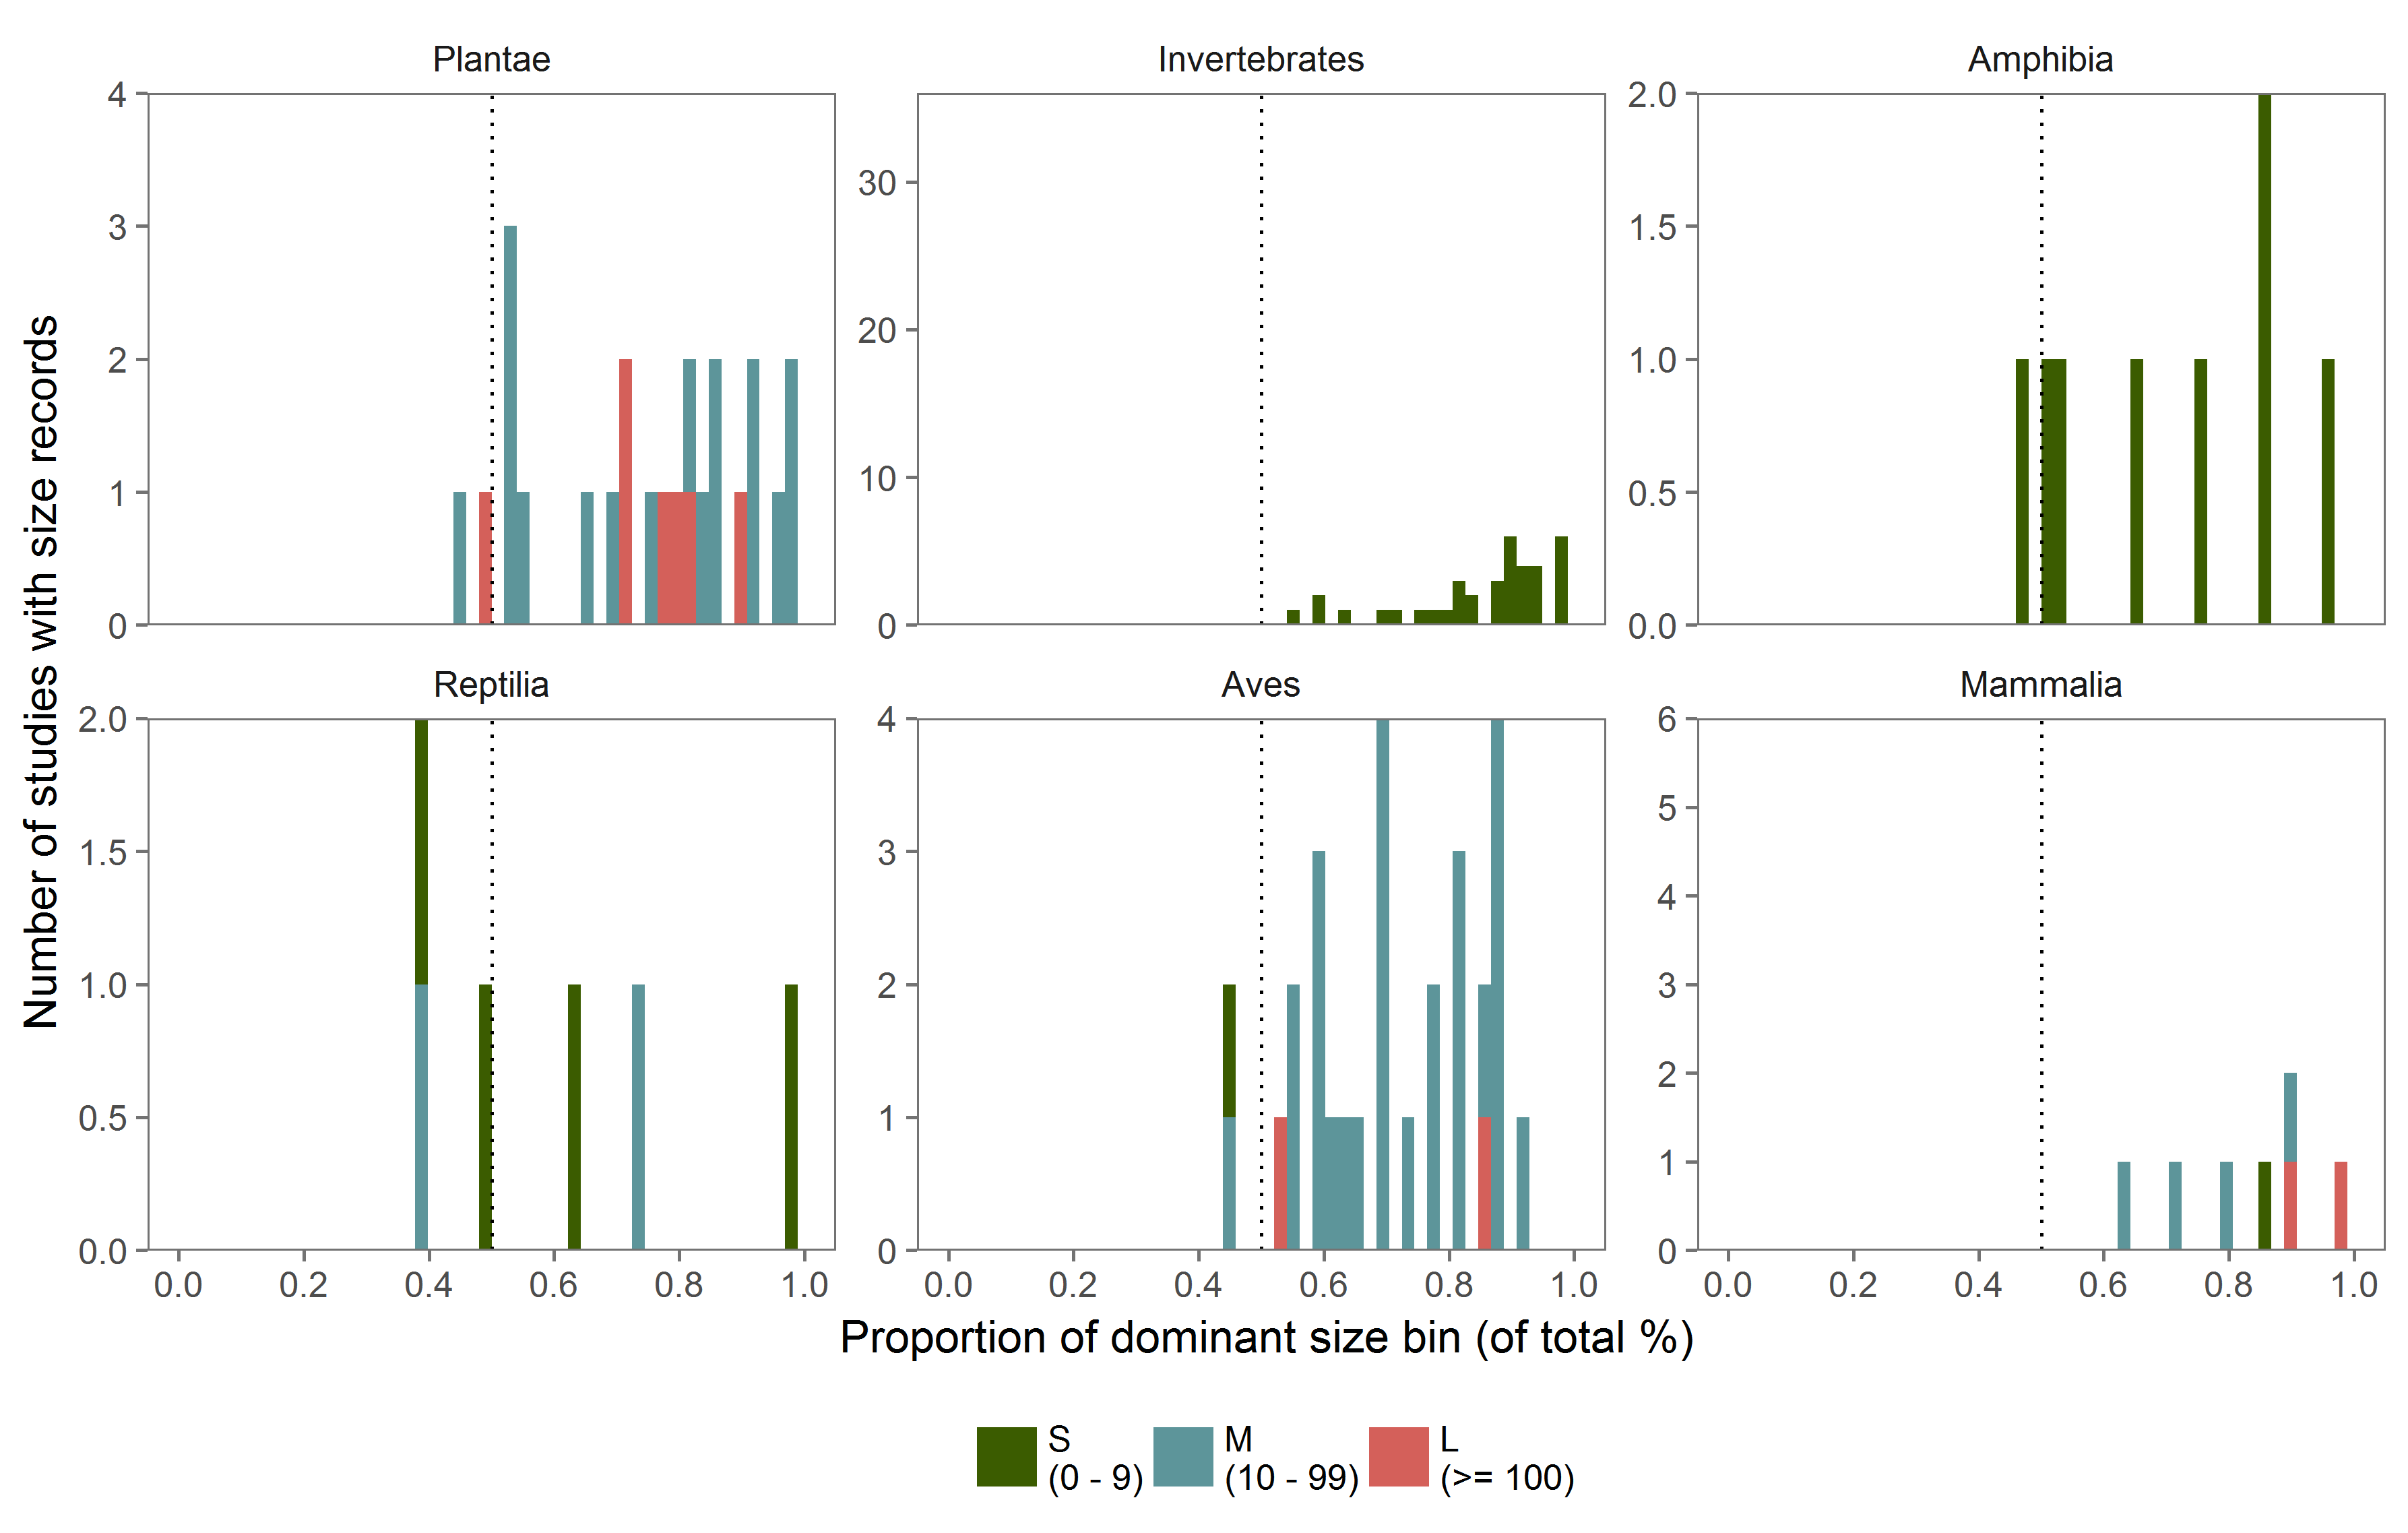
\includegraphics[width=1\textwidth]{chapter2/SI04}
\caption{ The proportion of species that contributed to a study being classified as either predominantly inhabited by small, medium or large species. The dotted line is a visual aid to assess simple majority (50\%) indicating whether a study classification is based on the majority of species within an assemblage. The y-axis shows the number of studies with similar proportions (note the difference in y-axis scale per taxonomic group). }
\label{SI02_04}
\end{figure}

% ------ %
% Regression table
\begin{sidewaystable}[h]
%\begin{table}[htb]
\centering
\caption{Averaged fixed effect, standard error (SE), marginal and conditional $R^2$ estimates as well as relative change in $R^2$ to current BC\textunderscript{EVI} of the overall average model (Figure \ref{F02_03}). N and N\textunderscript{sites} indicate the maximum number of studies and sites across permutations contributing to these estimates. }
\label{SIT02_01}
\begin{tabular}{llllllll}
\hline
Time Period & Slope & SE    & Marginal $R^{2}$ & Conditional $R^{2}$ & Relative difference $R^{2}$ & N   & N\textunderscript{sites} \\ \hline
yr\textunderscript{0}           & 0.289 & 0.064 & 0.012       & 0.464          & 0                      & 198 & 4053   \\
yr\textunderscript{1}           & 0.279 & 0.062 & 0.011       & 0.460          & -9.6                   & 198 & 4053   \\
yr\textunderscript{1-2}           & 0.299 & 0.065 & 0.012       & 0.462          & 0.4                    & 198 & 4053   \\
yr\textunderscript{1-3}           & 0.316 & 0.067 & 0.013       & 0.462          & 9.1                    & 198 & 4053   \\
yr\textunderscript{1-4}           & 0.323 & 0.069 & 0.013       & 0.463          & 11.2                   & 198 & 4053   \\
yr\textunderscript{1-5}           & 0.334 & 0.071 & 0.014       & 0.463          & 16.7                   & 198 & 4053   \\ \hline
\end{tabular}
\end{sidewaystable}
%\end{table}
% ------ %

% SI - Figure 5 Plot per taxonomic group
\begin{figure}[htb]
\centering
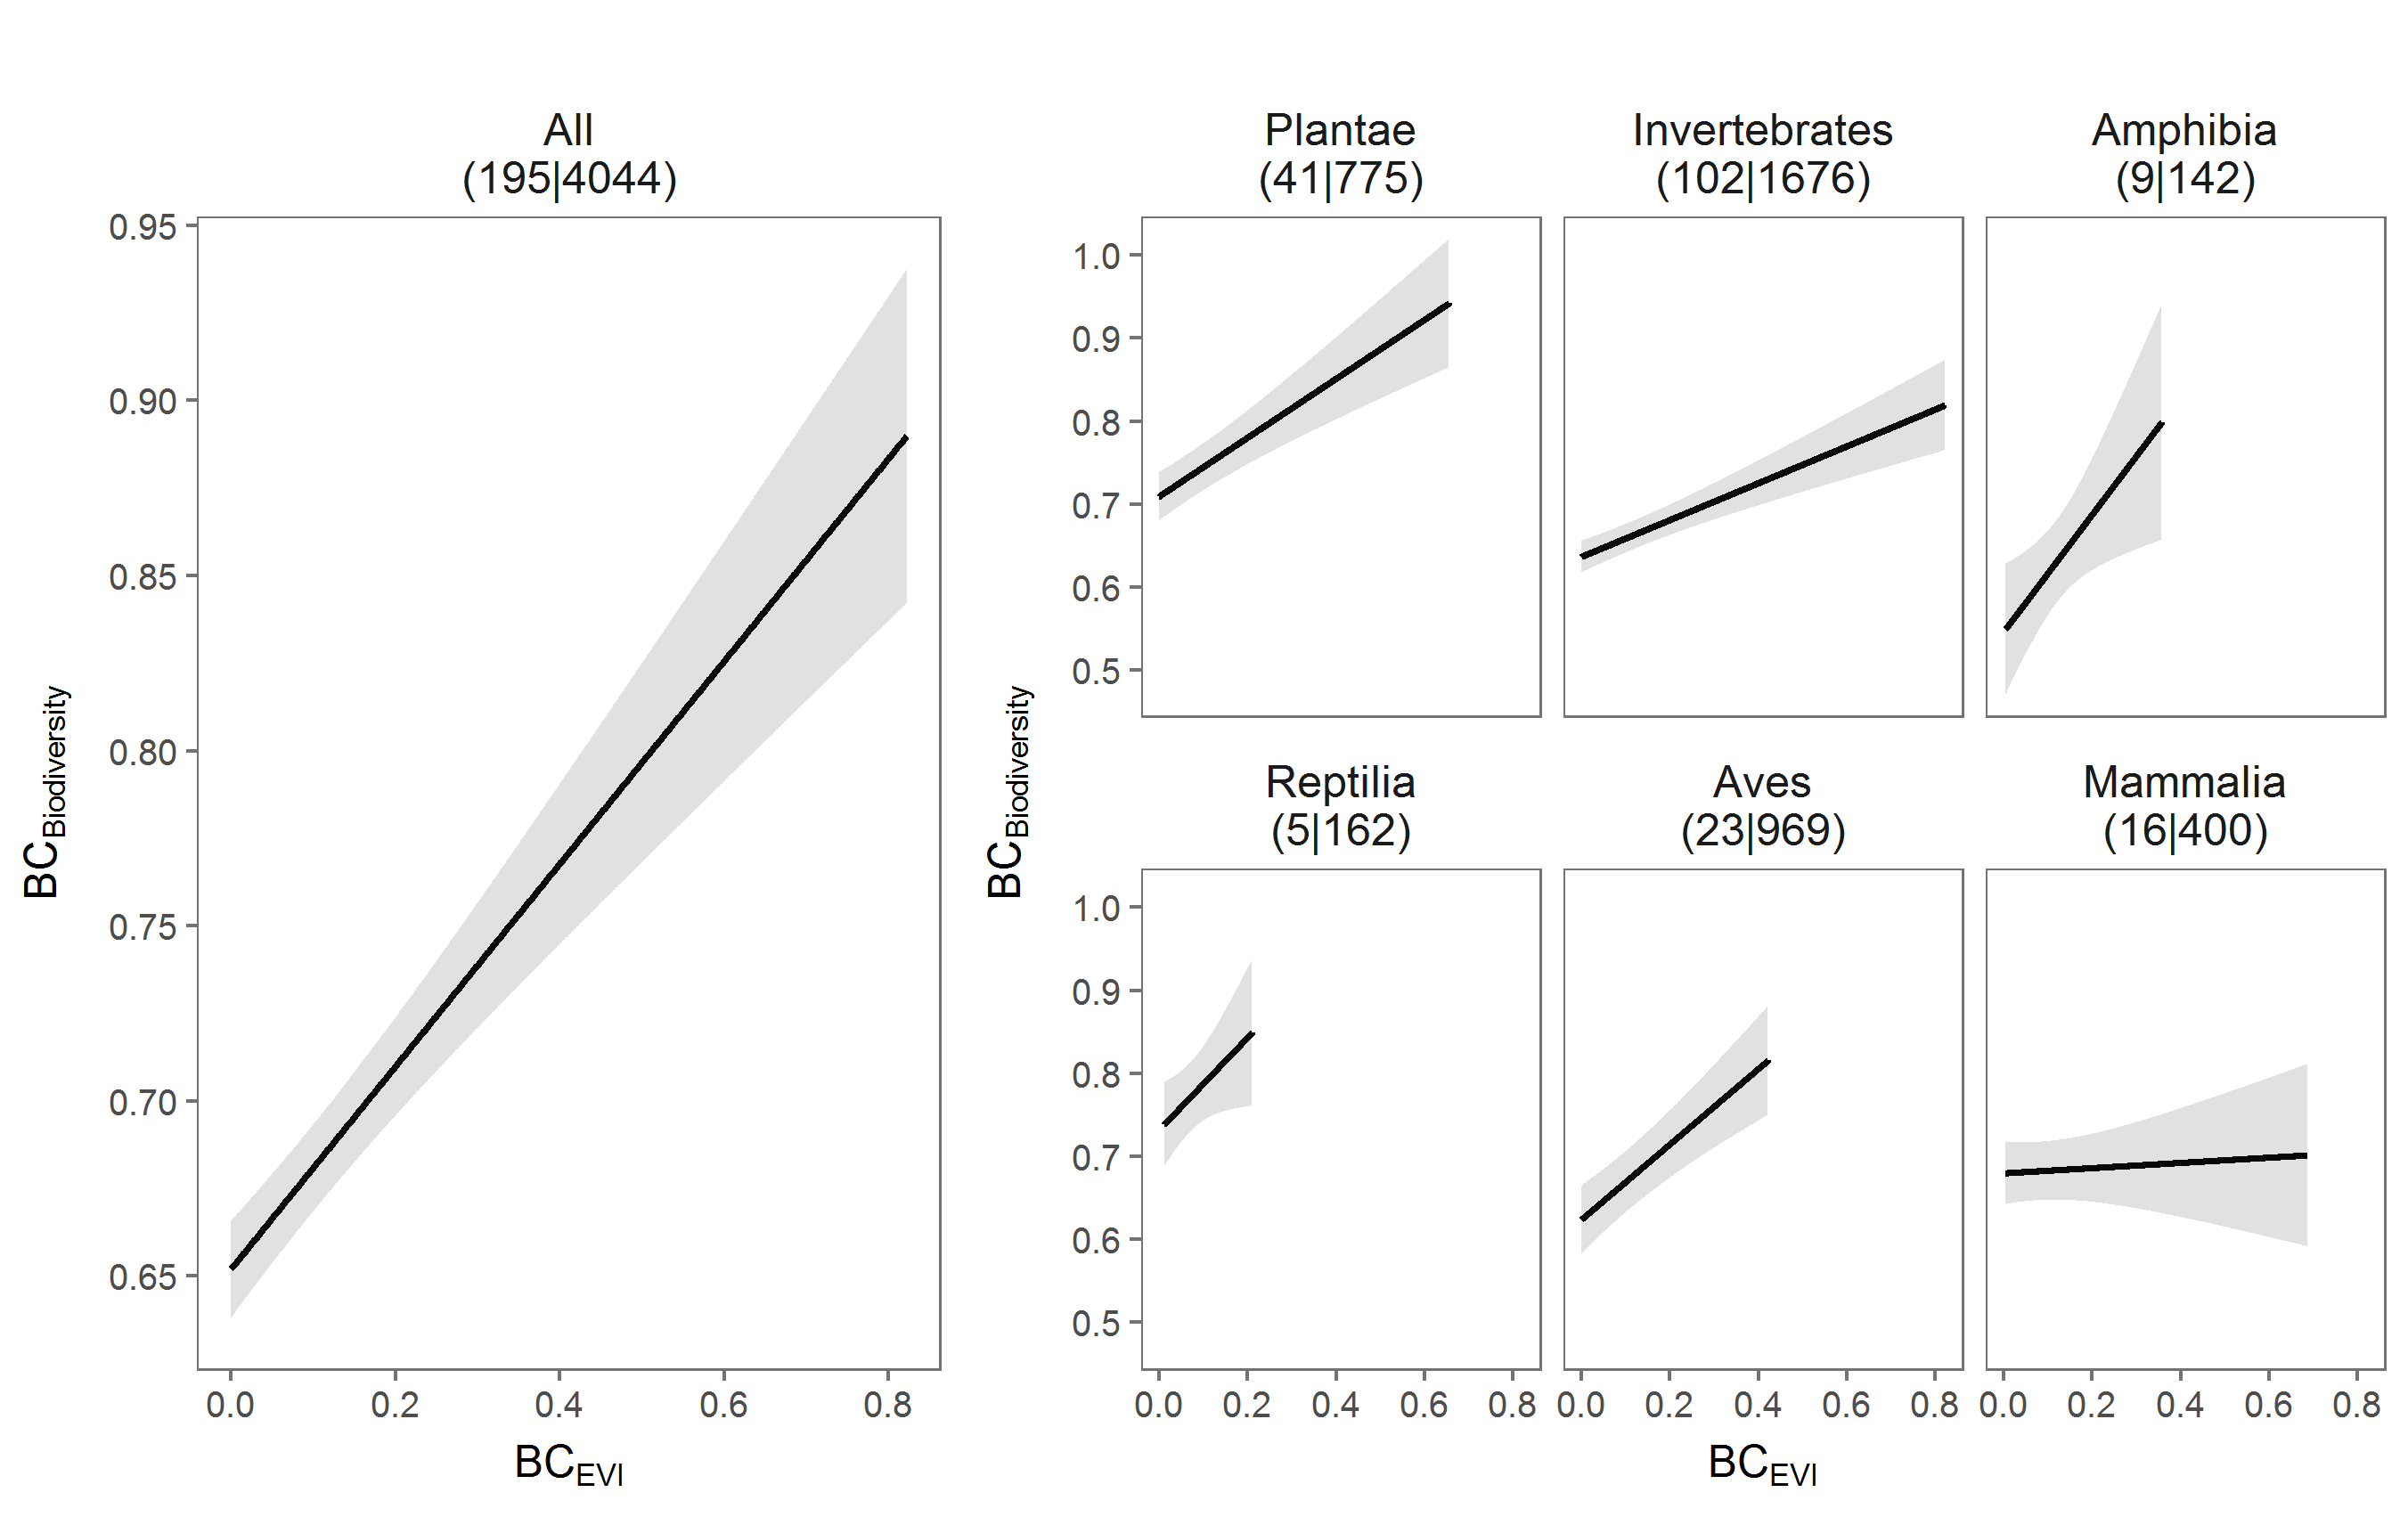
\includegraphics[width=1\textwidth]{chapter2/SI05}
\caption{ Effect of differences in current BC\textunderscript{EVI} in the first year before biodiversity sampling against their pairwise differences in species assemblages (BC\textunderscript{Biodiversity}). The number of studies and contributing sites (N|N\textunderscript{Sites}) is indicated for each taxonomic group. }
\label{SI02_05}
\end{figure}

% SI - Figure 6 Simulation
\begin{figure}[htb]
\centering
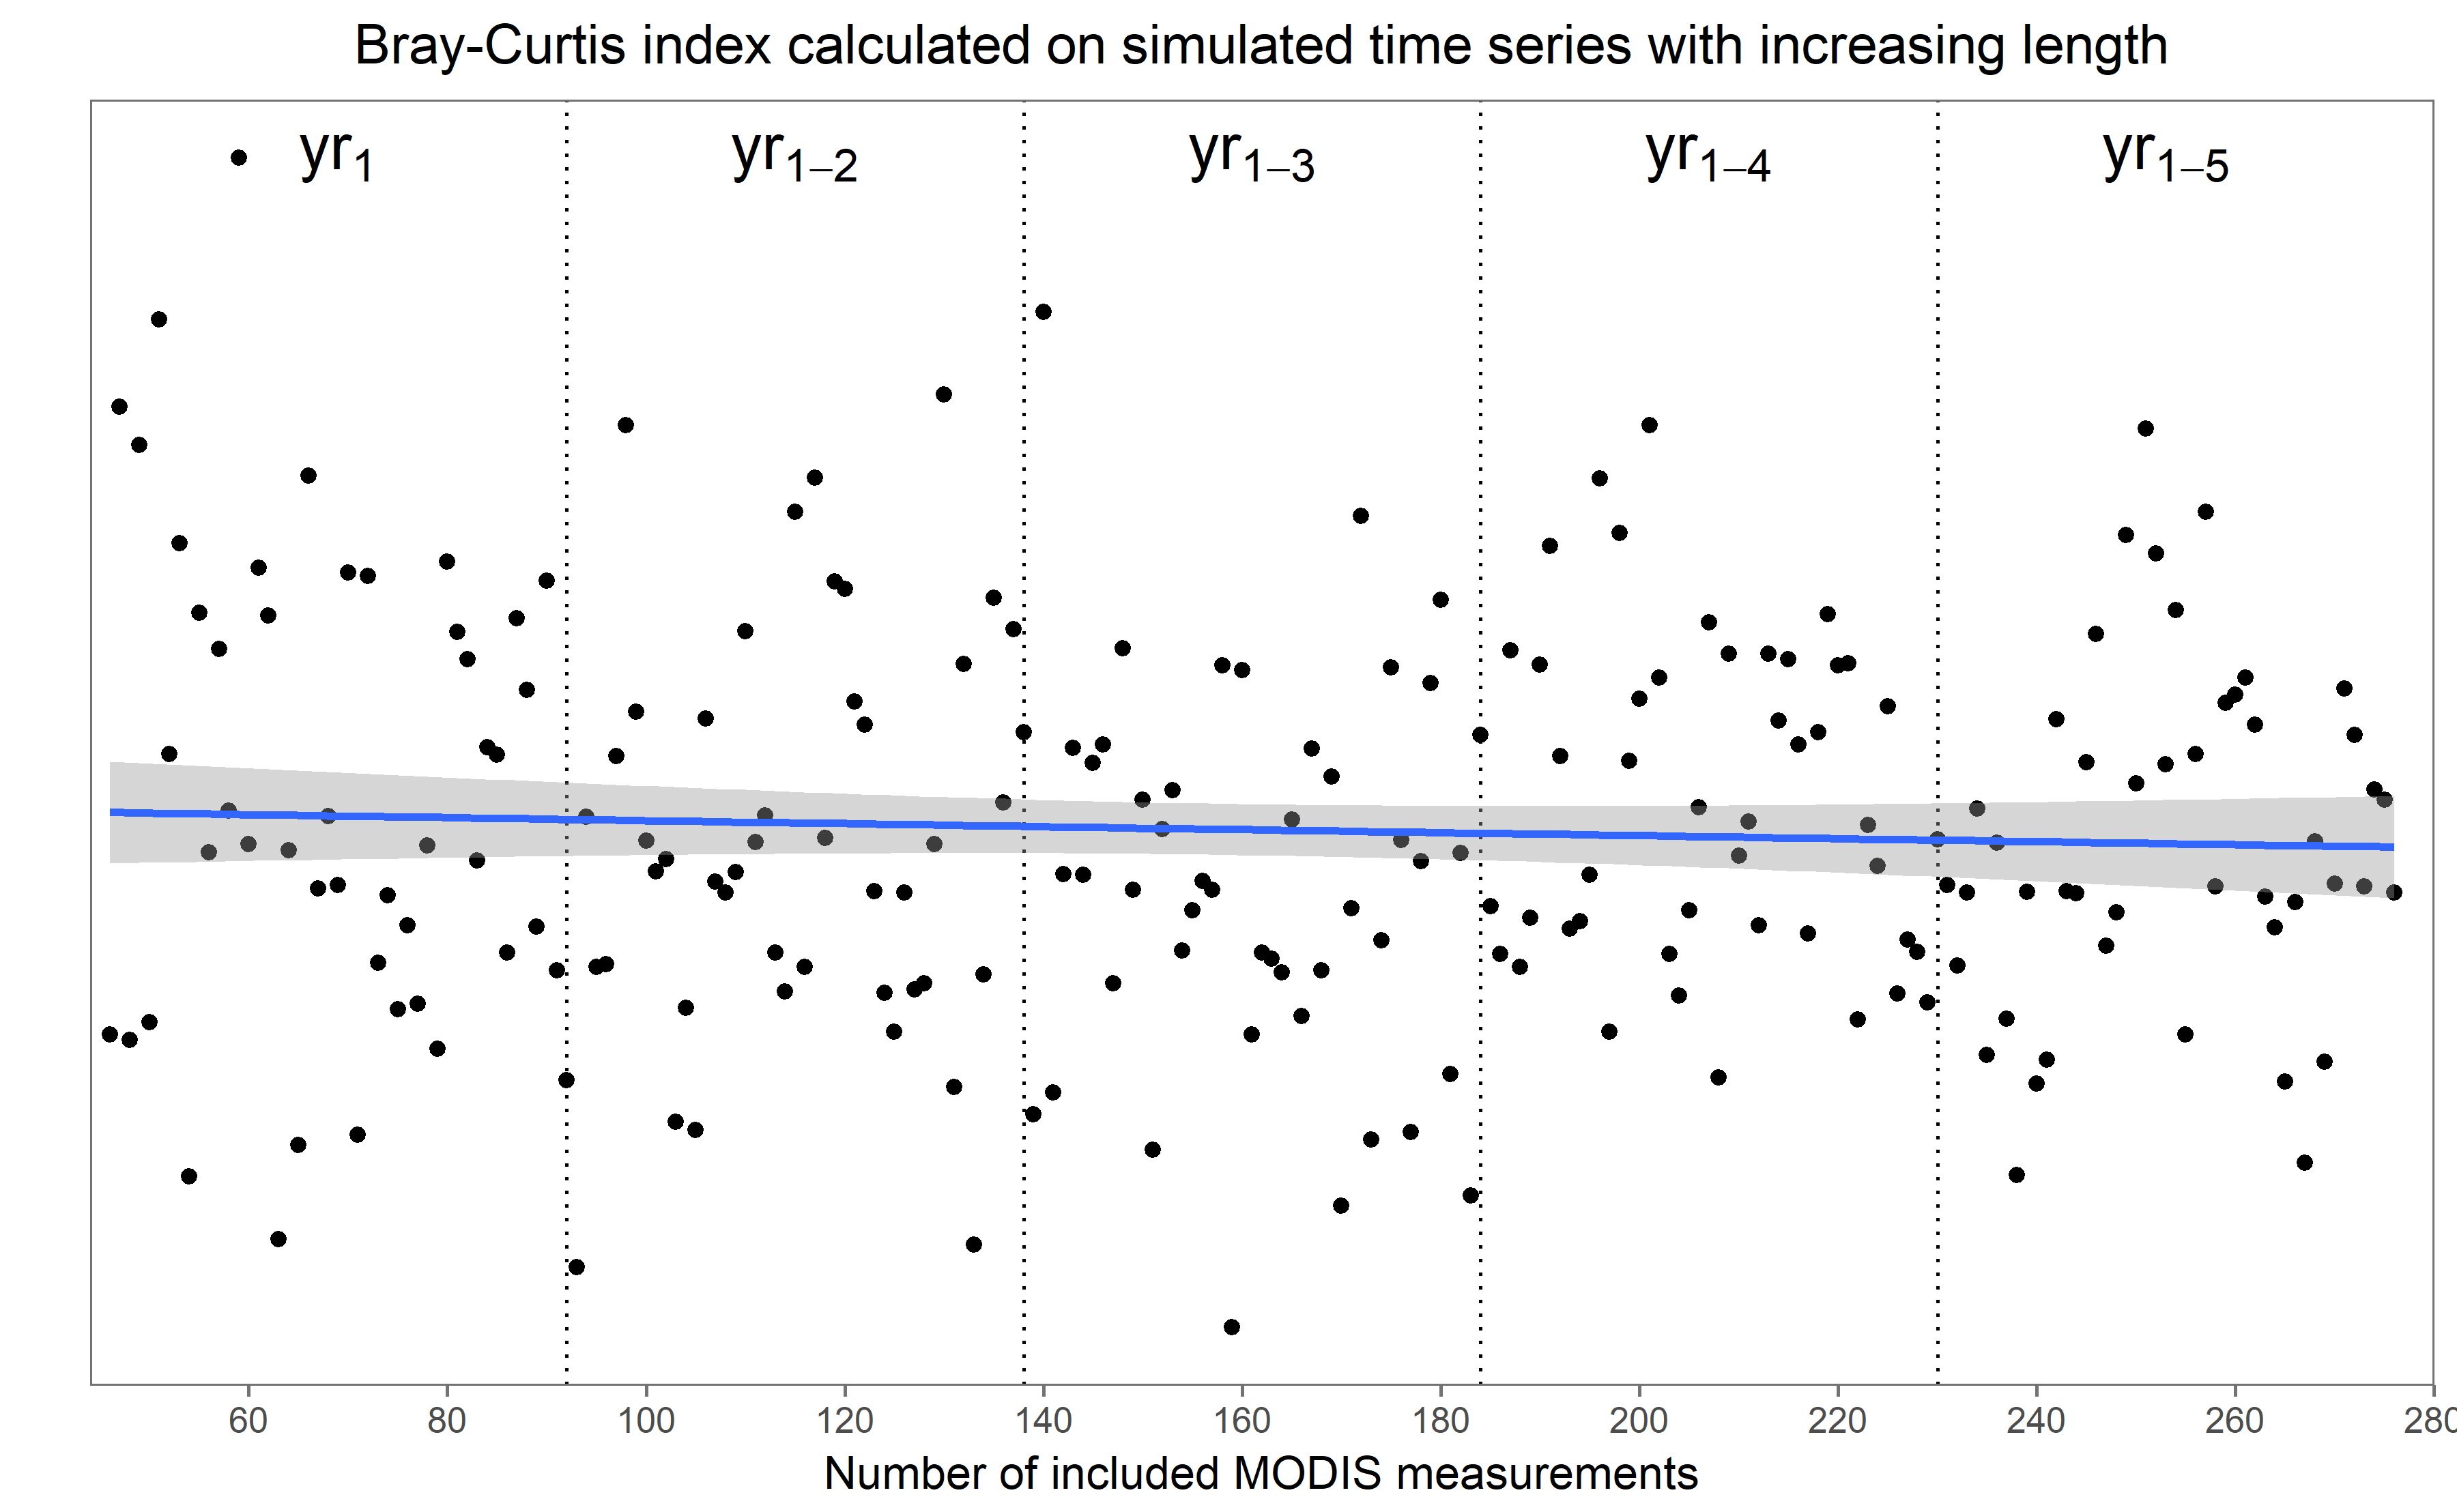
\includegraphics[width=1\textwidth]{chapter2/SI06}
\caption{ Simulation of how the Bray-Curtis index (BC\textunderscript{EVI}) between two time series changes with increasing time series length. Calculated on pairs of randomly generated time series for each past period. Vertical dotted lines indicate periods of full past years of theoretical possible MODIS measurements (46 each, increasing from 46 initially for current BC\textunderscript{EVI}). There is no overall bias that the Bray-Curtis index increases with time series length (blue line shows a linear regression fit; $\beta$ < 0.0001, df = 229, p = 0.44).}
\label{SI02_06}
\end{figure}

% SI - Figure 7 Spatial autocorrelation
\begin{figure}[htb]
\centering
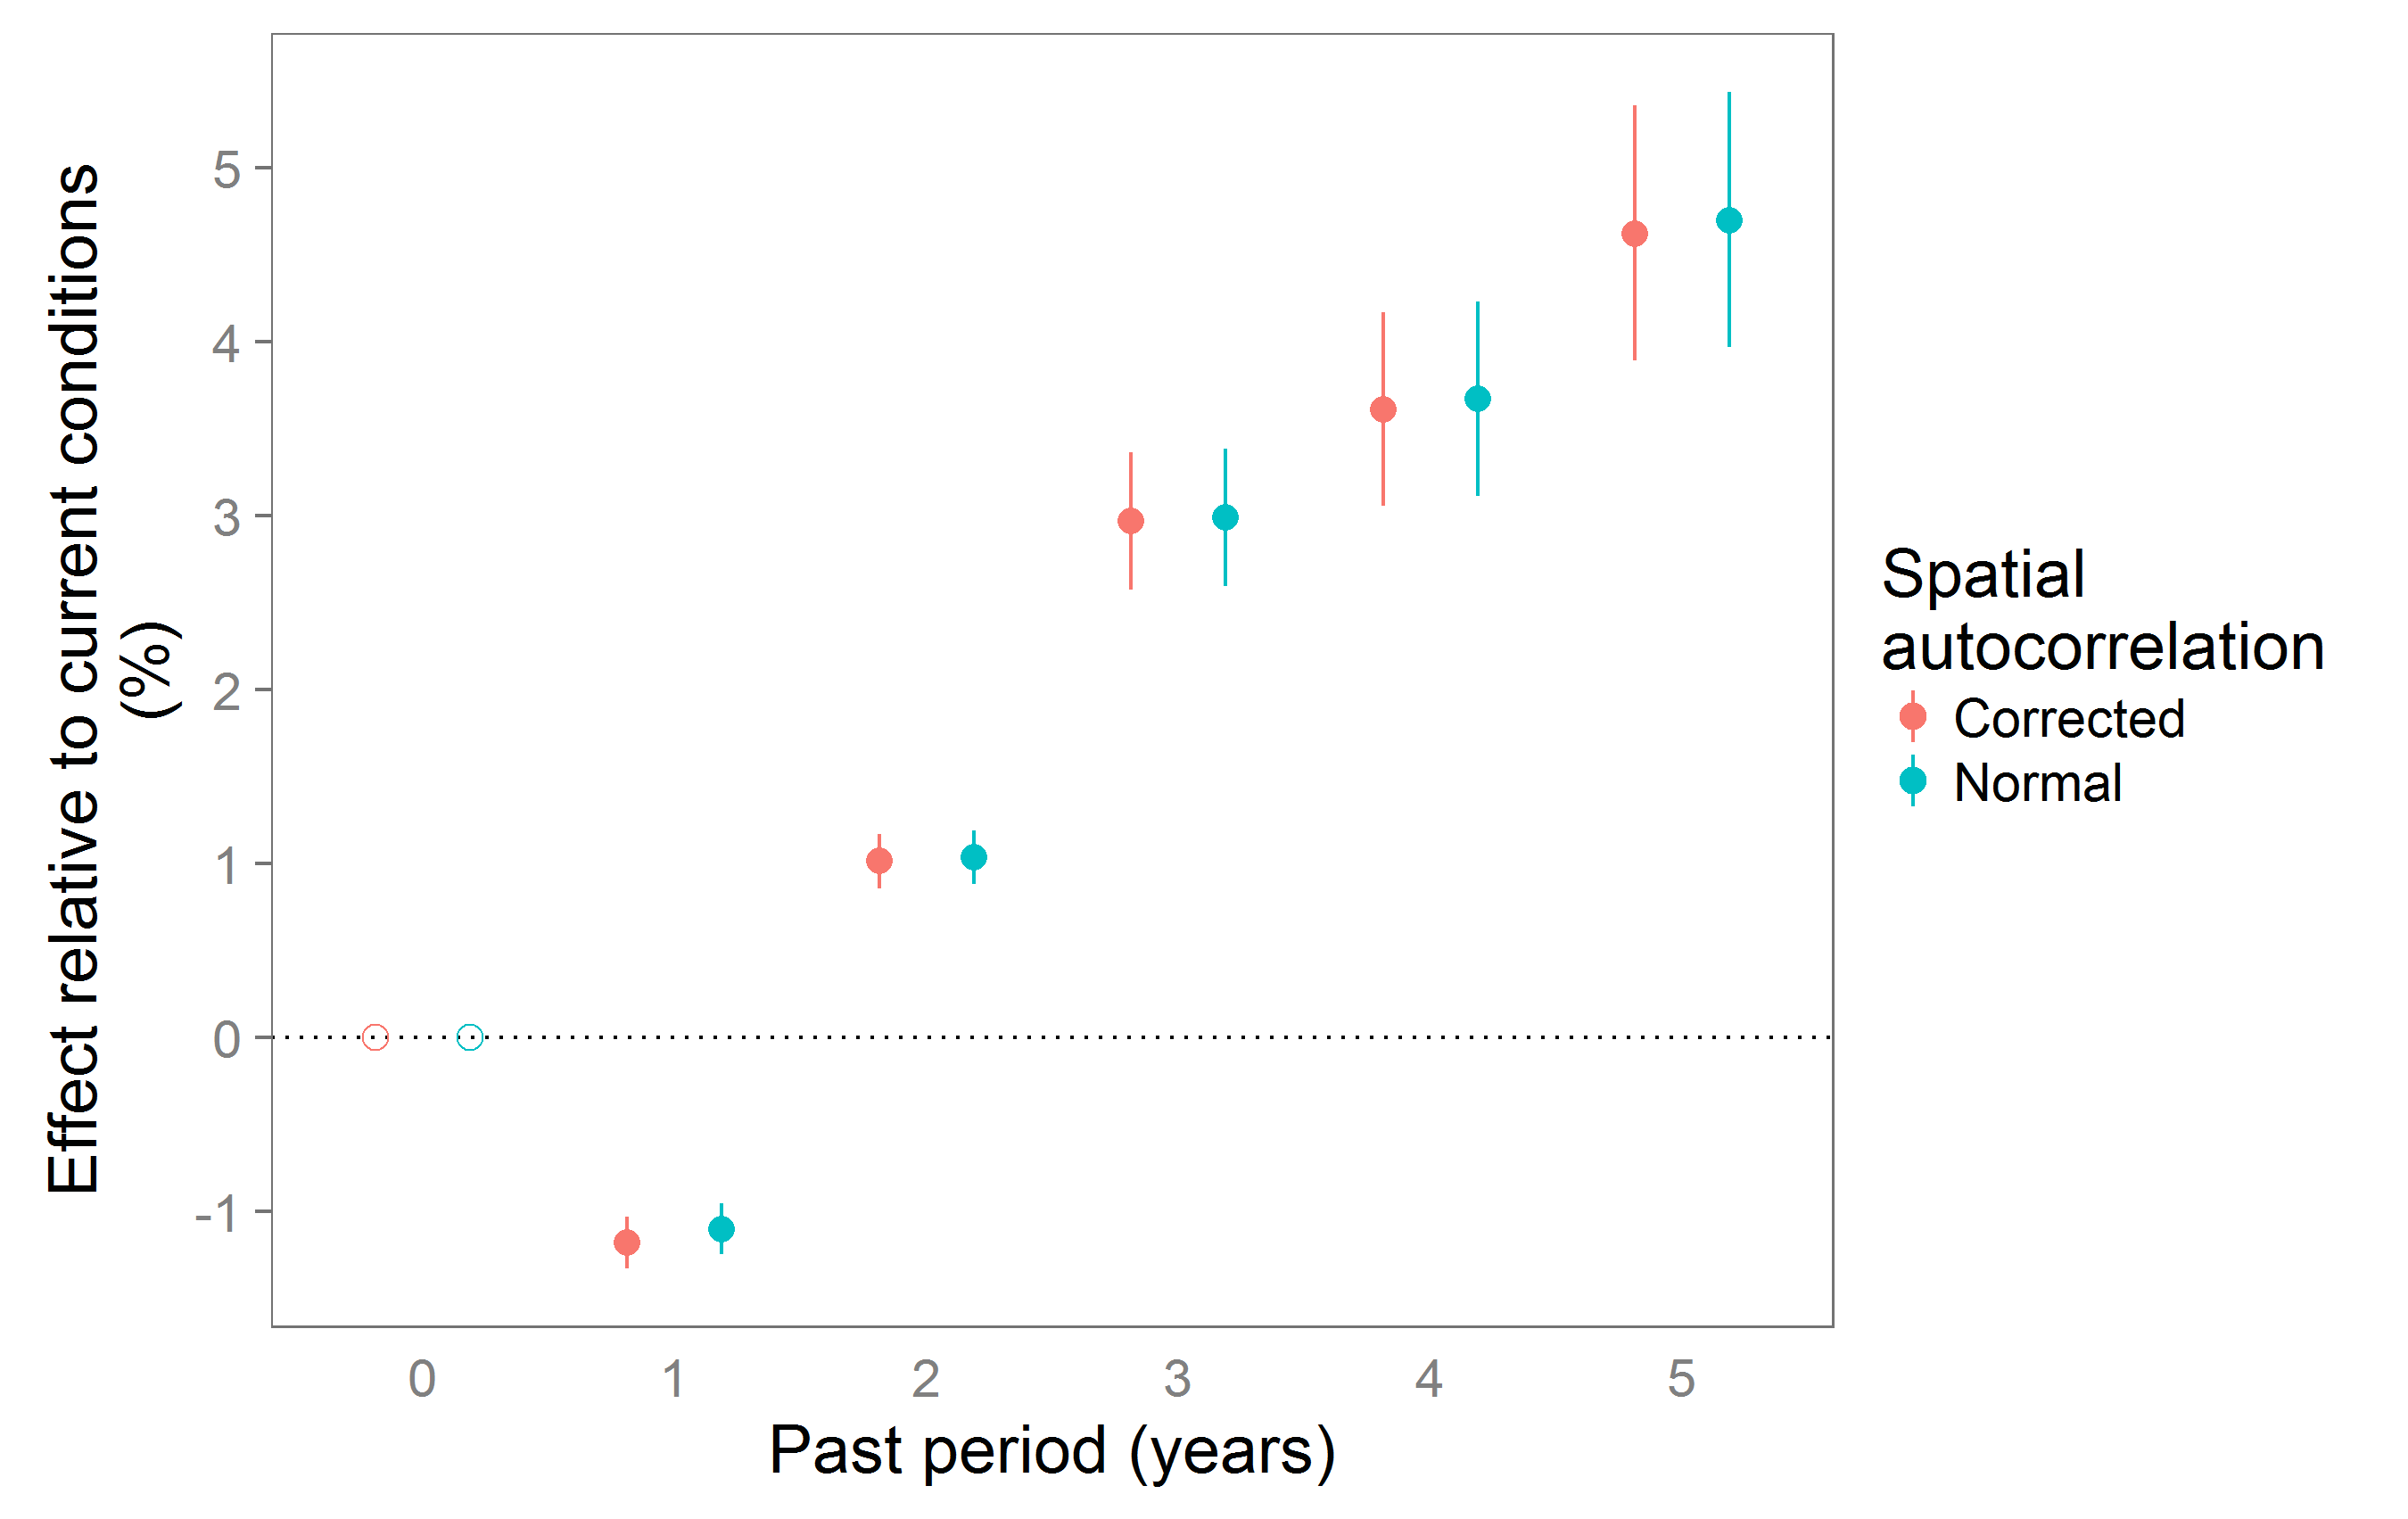
\includegraphics[width=1\textwidth]{chapter2/SI07}
\caption{ Difference in overall fit if studies with significant residual correlation with spatial distance (N=1) are removed. X-axis shows the current (0) and past periods (yr\textunderscript{1-5}), while the y-axis shows the difference in effect relative to the effect of current BC\textunderscript{EVI}.}
\label{SI02_07}
\end{figure}

% SI - Figure 8 Any biases
\begin{figure}[htb]
\centering
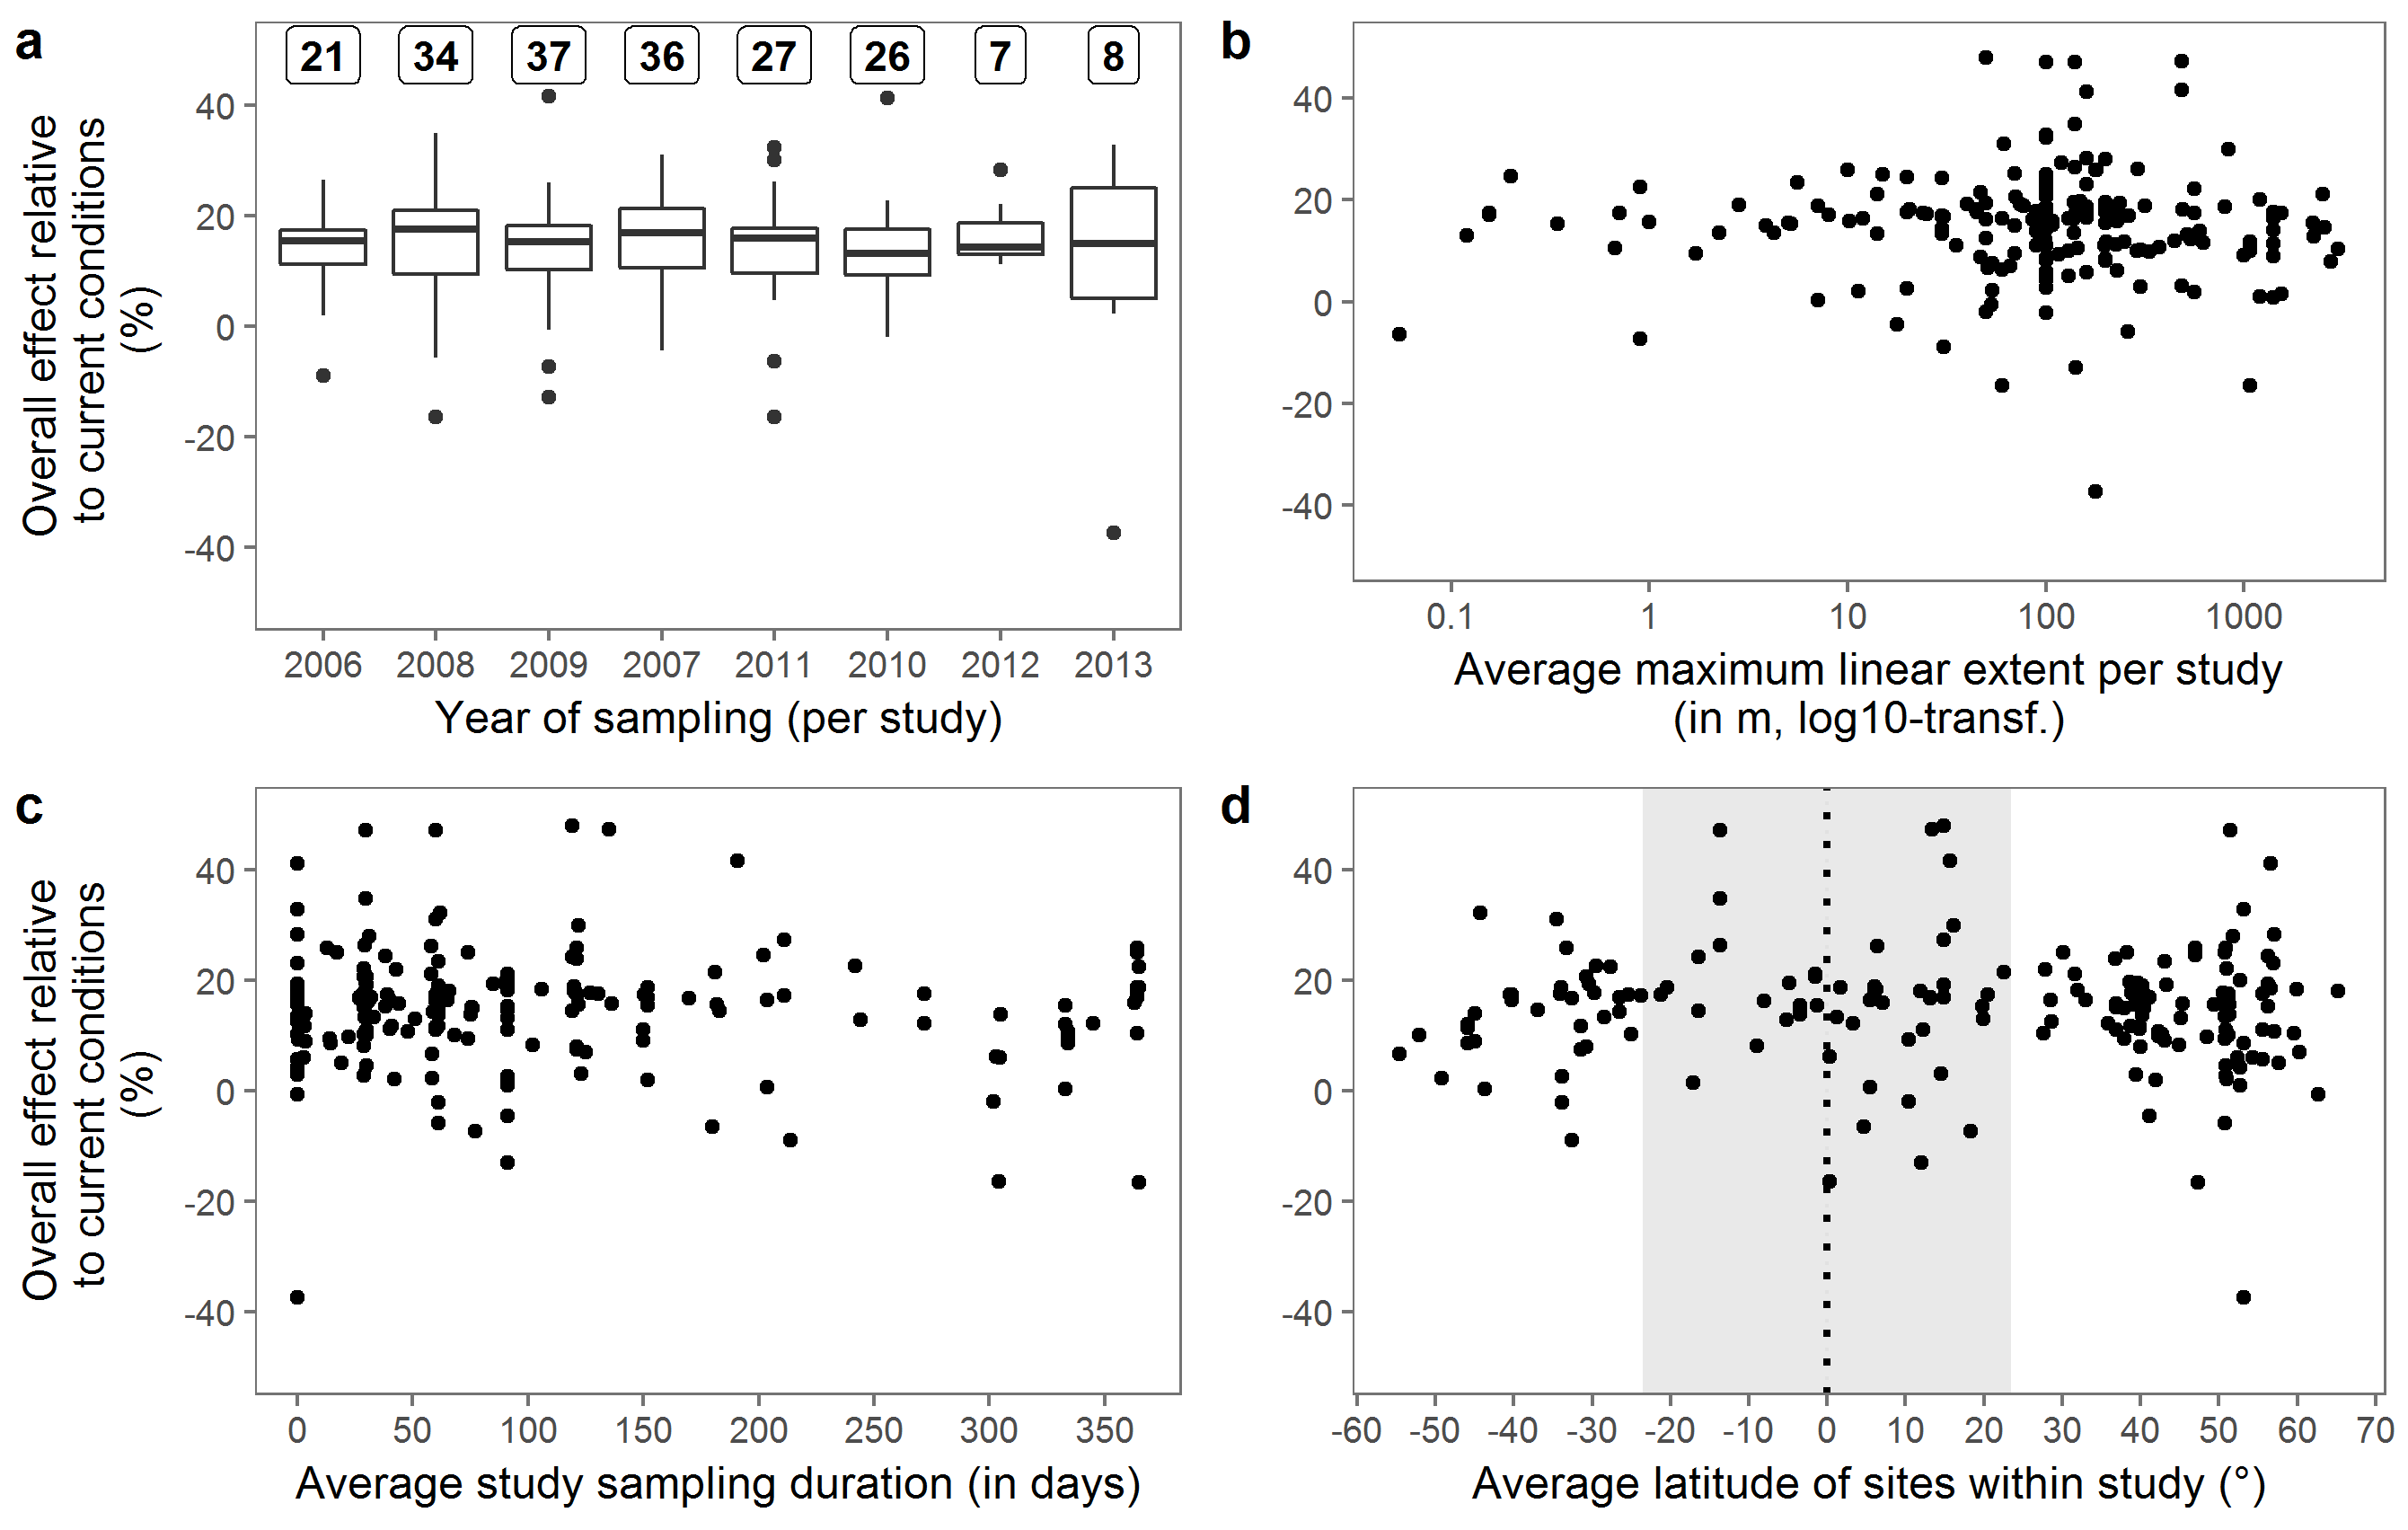
\includegraphics[width=1\textwidth]{chapter2/SI08}
\caption{ Investigation of potential broad-scale biases of the full model coefficients (5-year period). There is no bias in the permuted model effects with regards to (\textbf{a}) year of biodiversity sampling, (\textbf{b}) spatial scale of sampling, (\textbf{c}) average sampling duration, or (\textbf{d}) average latitude of study (grey shading indicates tropic belt).}
\label{SI02_08}
\end{figure}

% SI - Figure 9 Using another metric
\begin{figure}[htb]
\centering
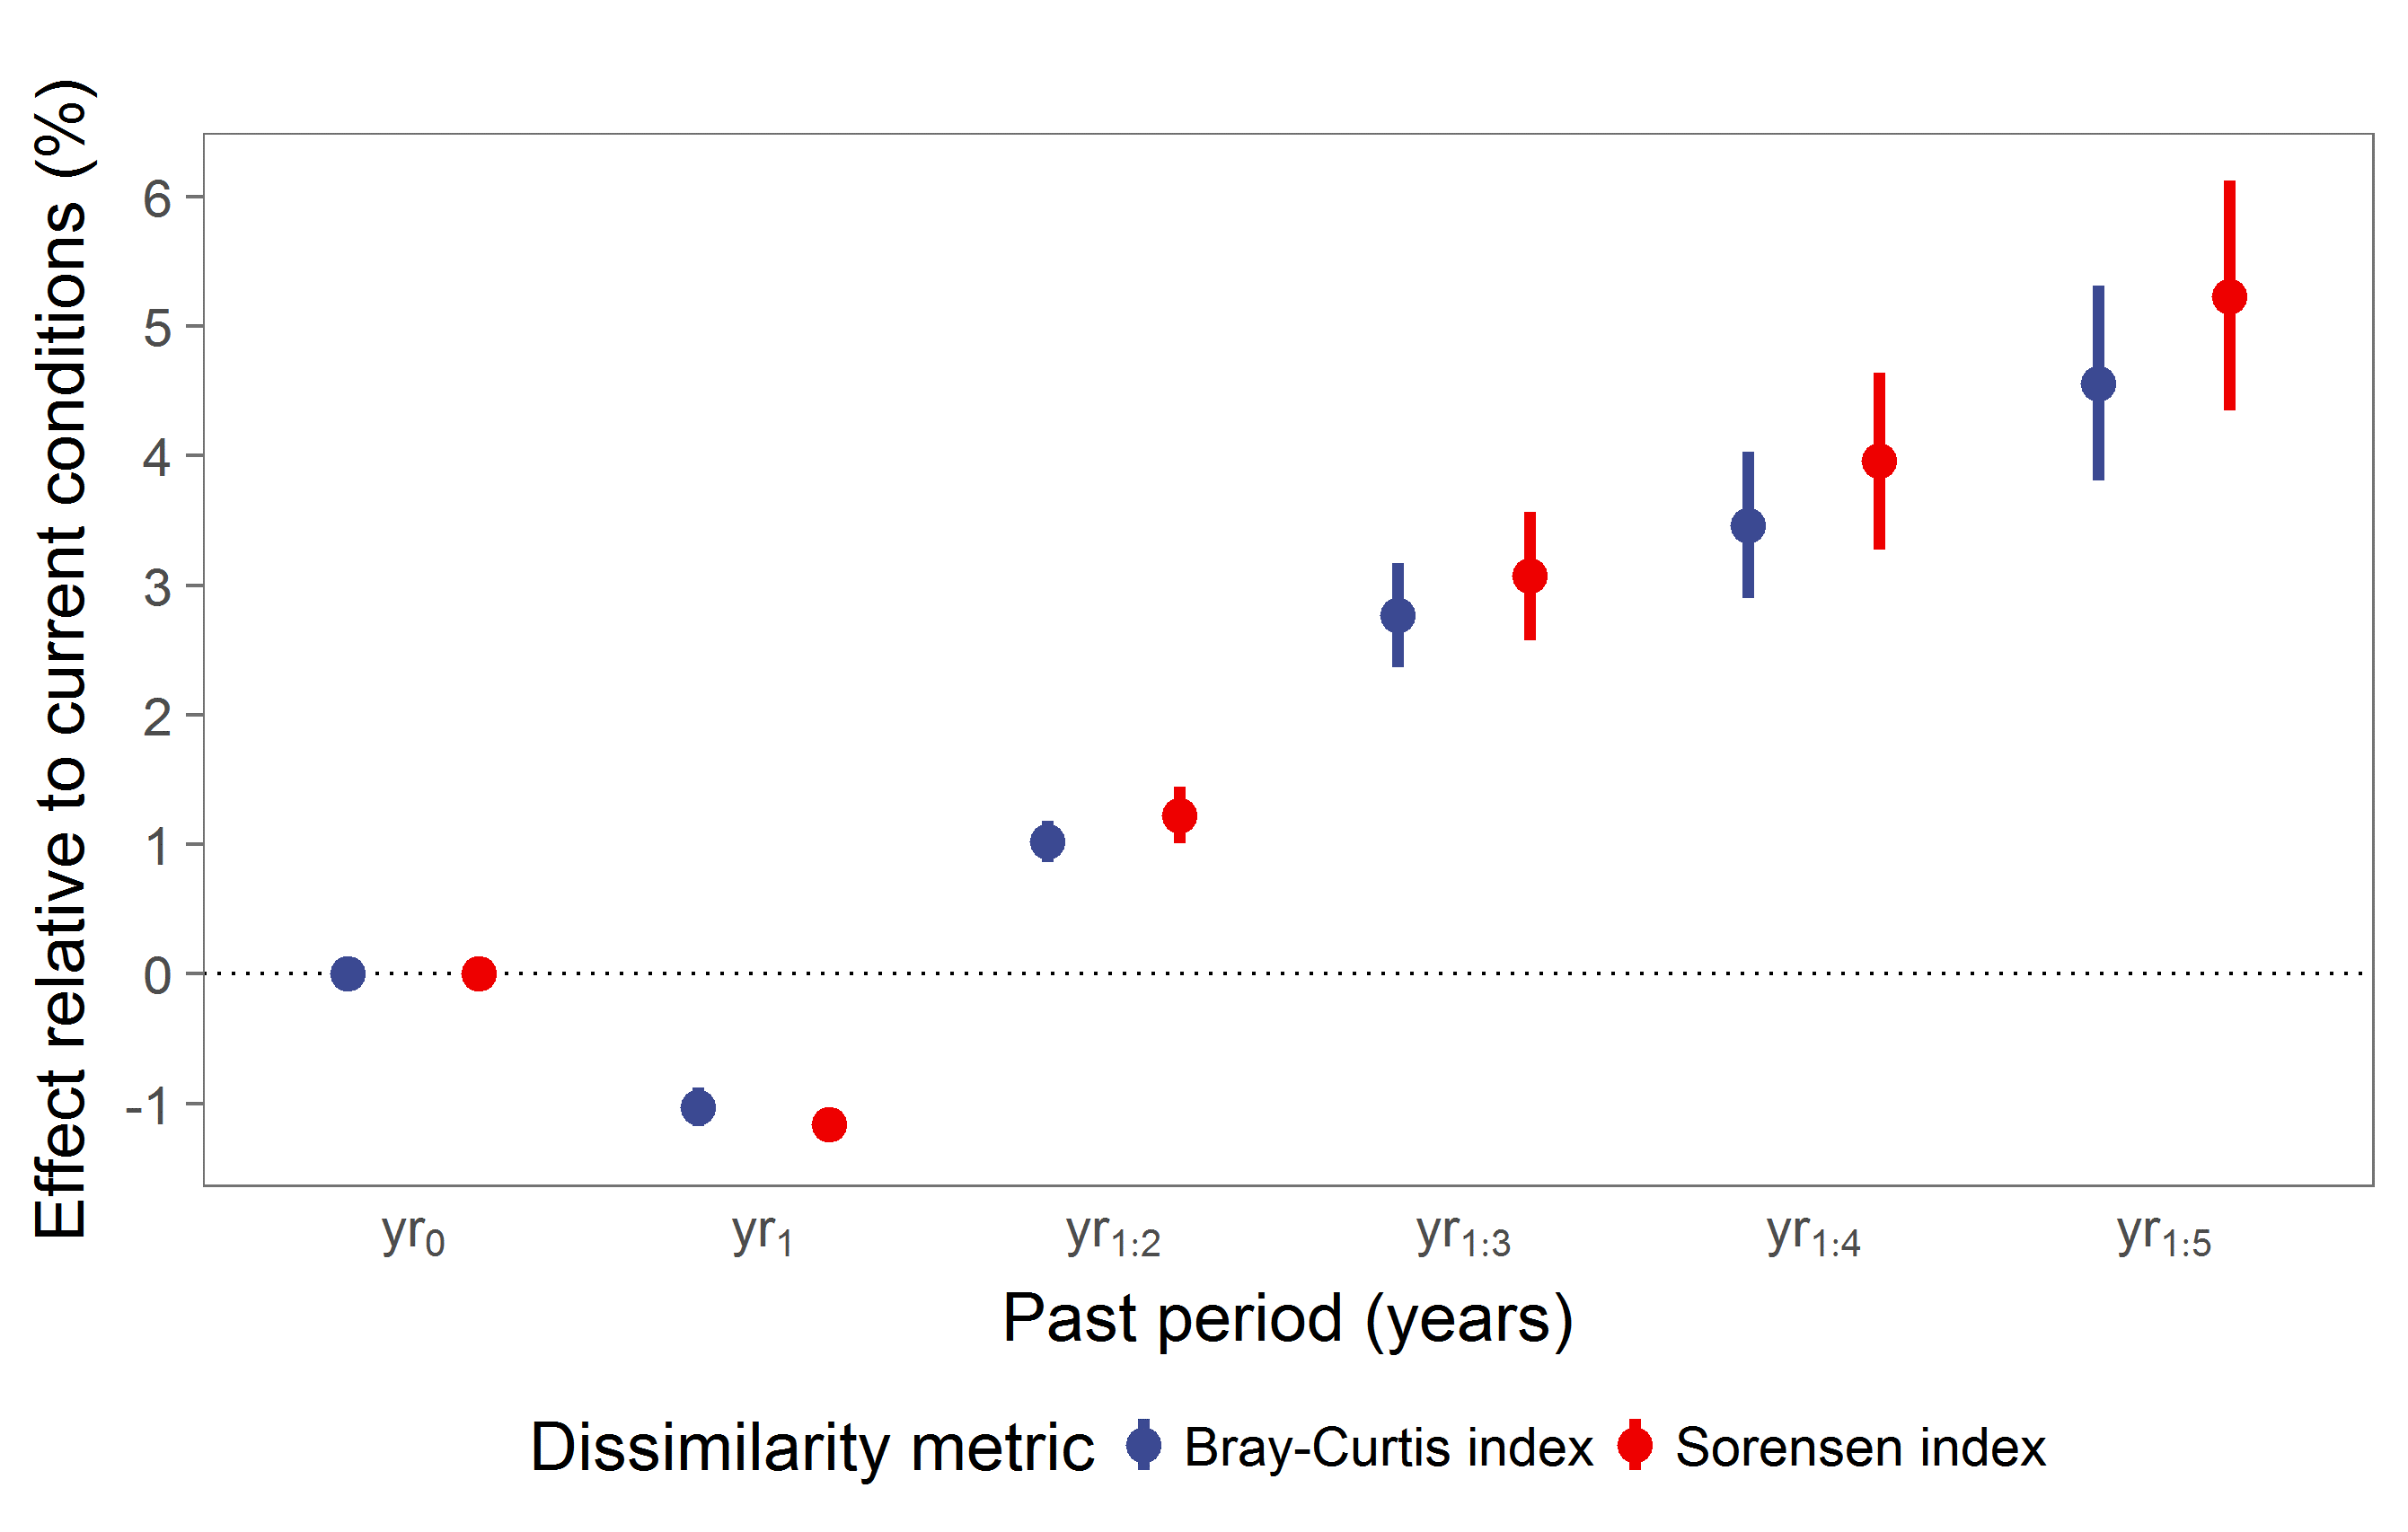
\includegraphics[width=1\textwidth]{chapter2/SI09}
\caption{ Overall influence of past periods of BC\textunderscript{EVI} on species assemblage composition as in Figure \ref{F02_03}, however shown for both Bray-Curtis index and as alternative the S\o rensen index. Axis labels as in Figure \ref{F02_03}.}
\label{SI02_09}
\end{figure}

  \section{Appendix - Chapter 3}
  % SI - Figure 1 Missing data
\begin{figure}[h]
\centering
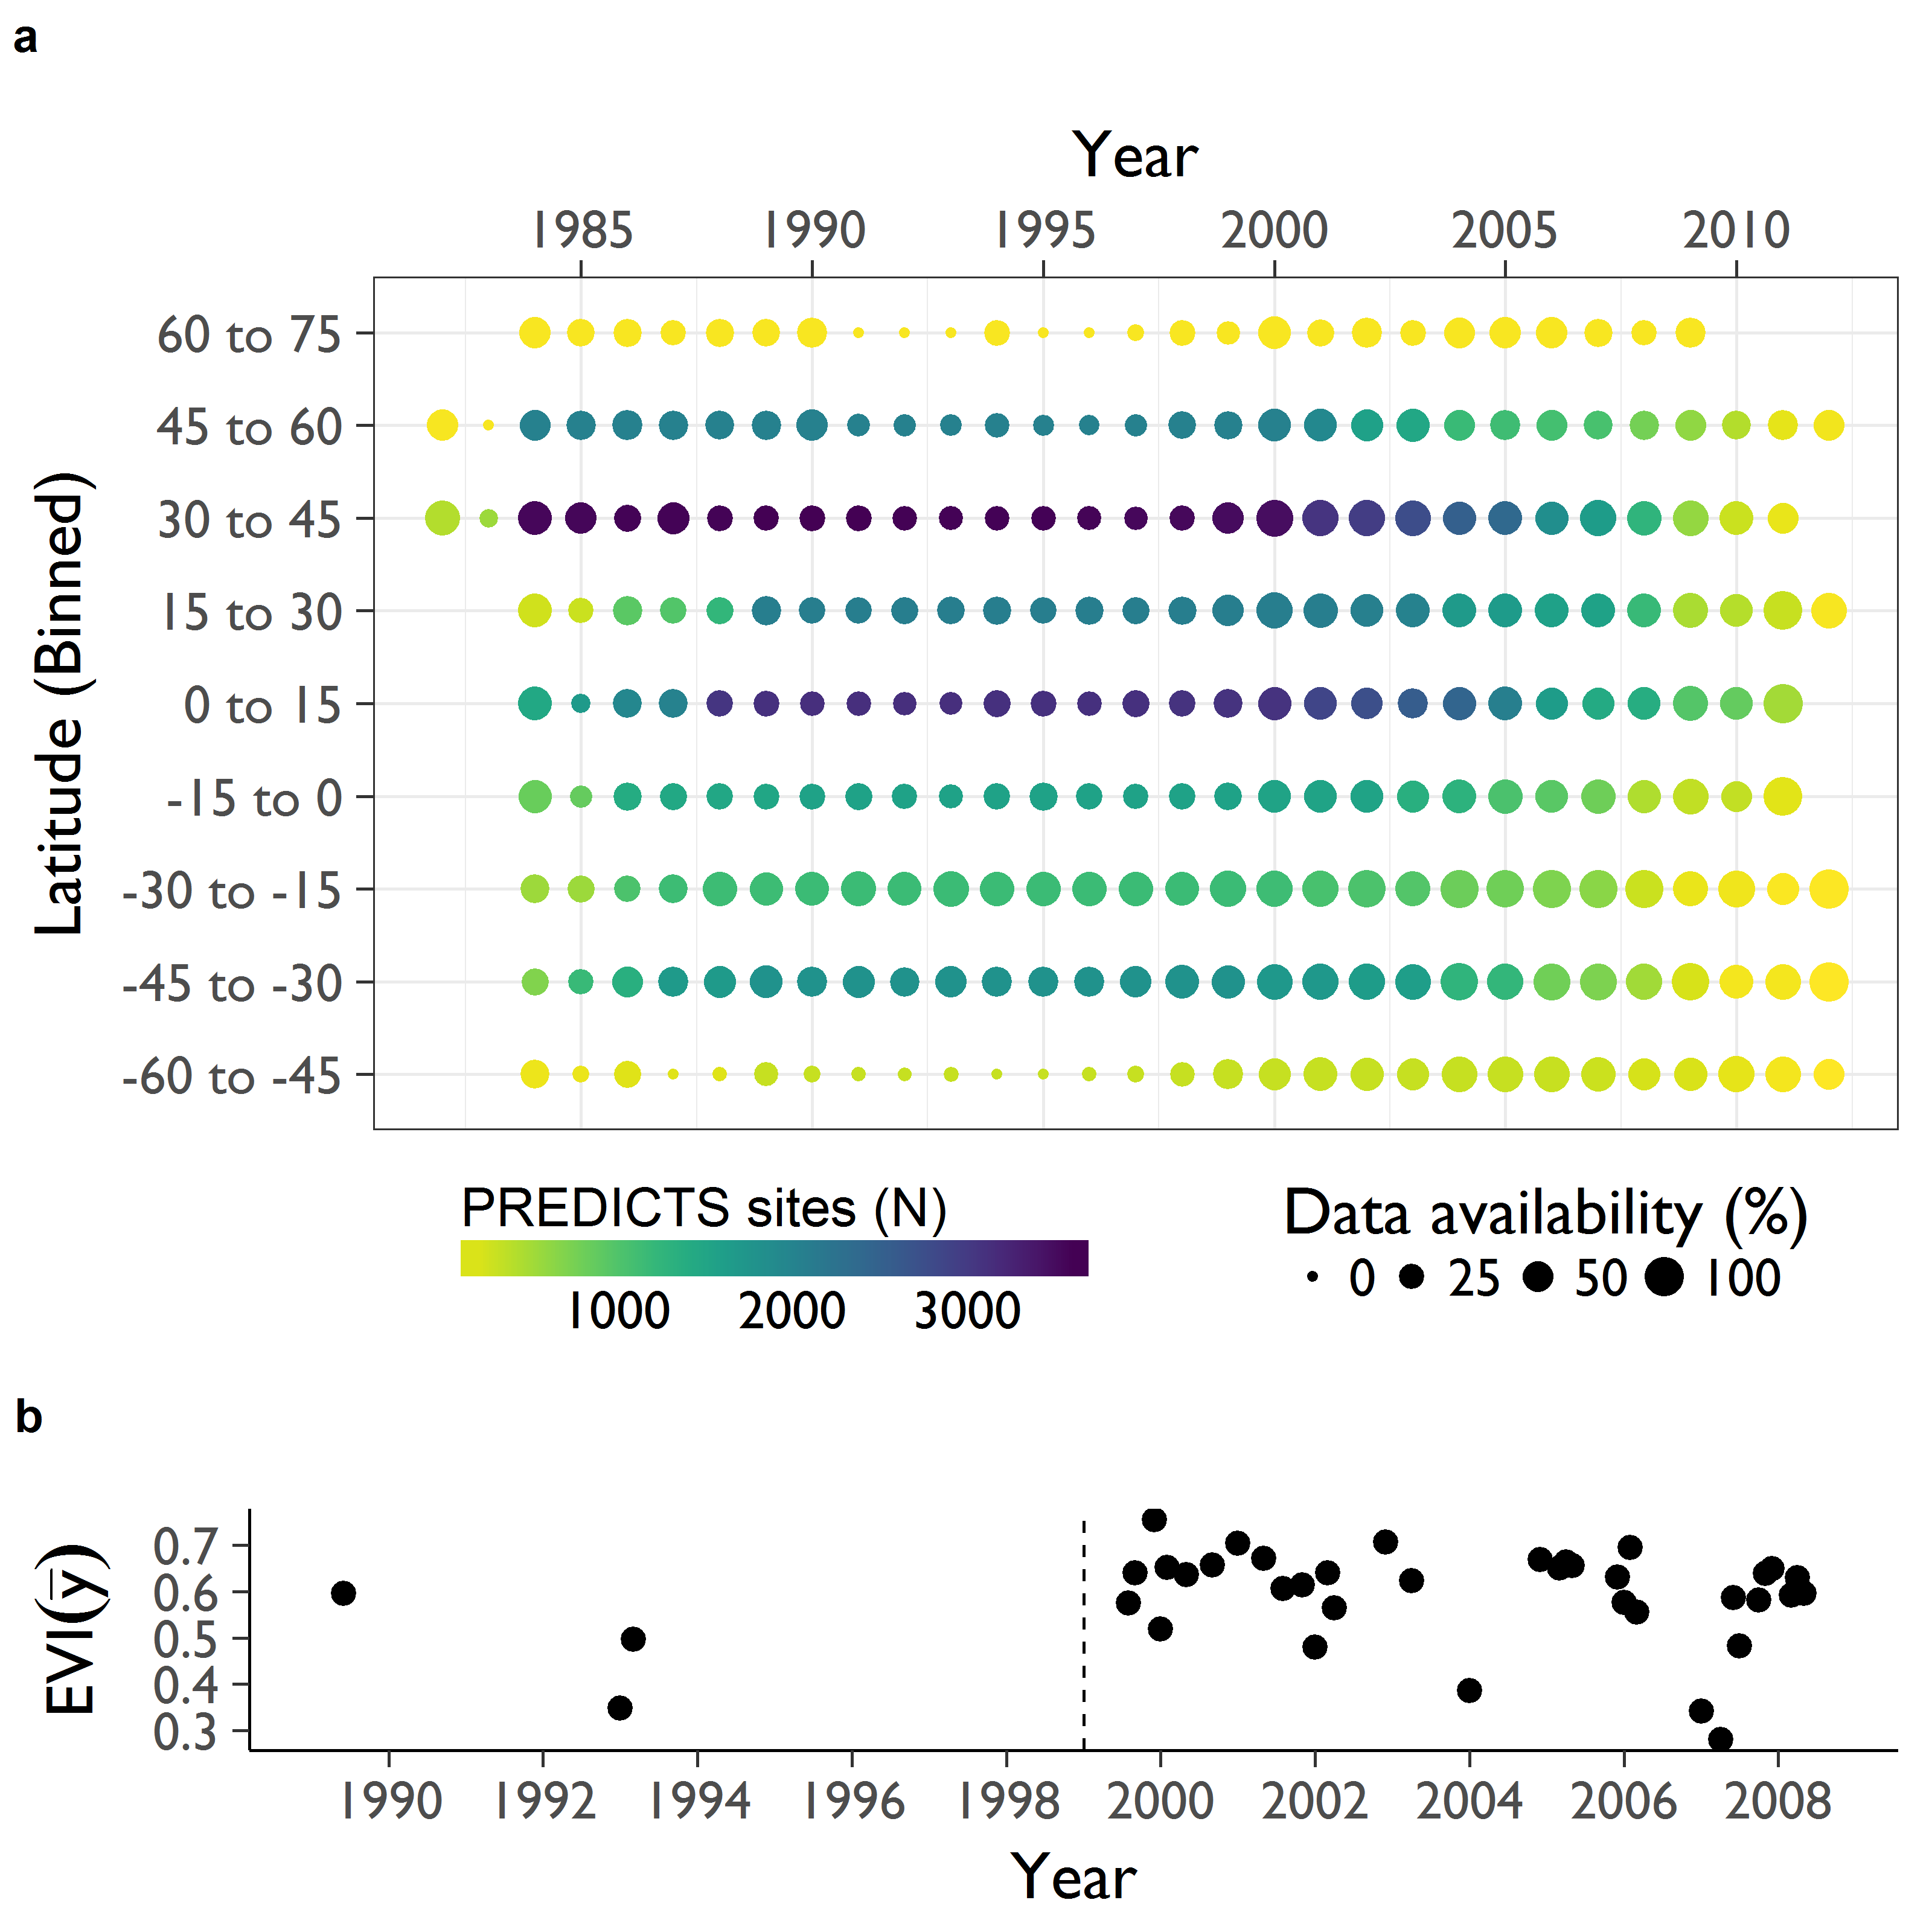
\includegraphics[width=1\textwidth]{chapter3/SI01}
\caption{ Average temporal distribution of Landsat data and an example times series of Landsat data. (\textbf{a}) Distribution of available Enhanced Vegetation Index (EVI) data in years covered by the Landsat missions. Points show the average monthly EVI data availability per year (0 to 12 months of data) across time series and PREDICTS sites grouped by 15\textdegree latitude bins. The size of points indicates the mean data availability (0 to 100\% with 100\% having 12 months of available data in a given year), while the colour shows the number of PREDICTS sites contributing to the mean (as PREDICTS sites were sampled in varying years). (\textbf{b}) Example time series for one PREDICTS site with a high proportion of missing data before 1999. In all analyses such time series were truncated to the period from 1999 onwards (indicated by the dashed line).}
\label{SI03_01}
\end{figure}

% SI - Figure 2 Binning
\begin{figure}[h]
\centering
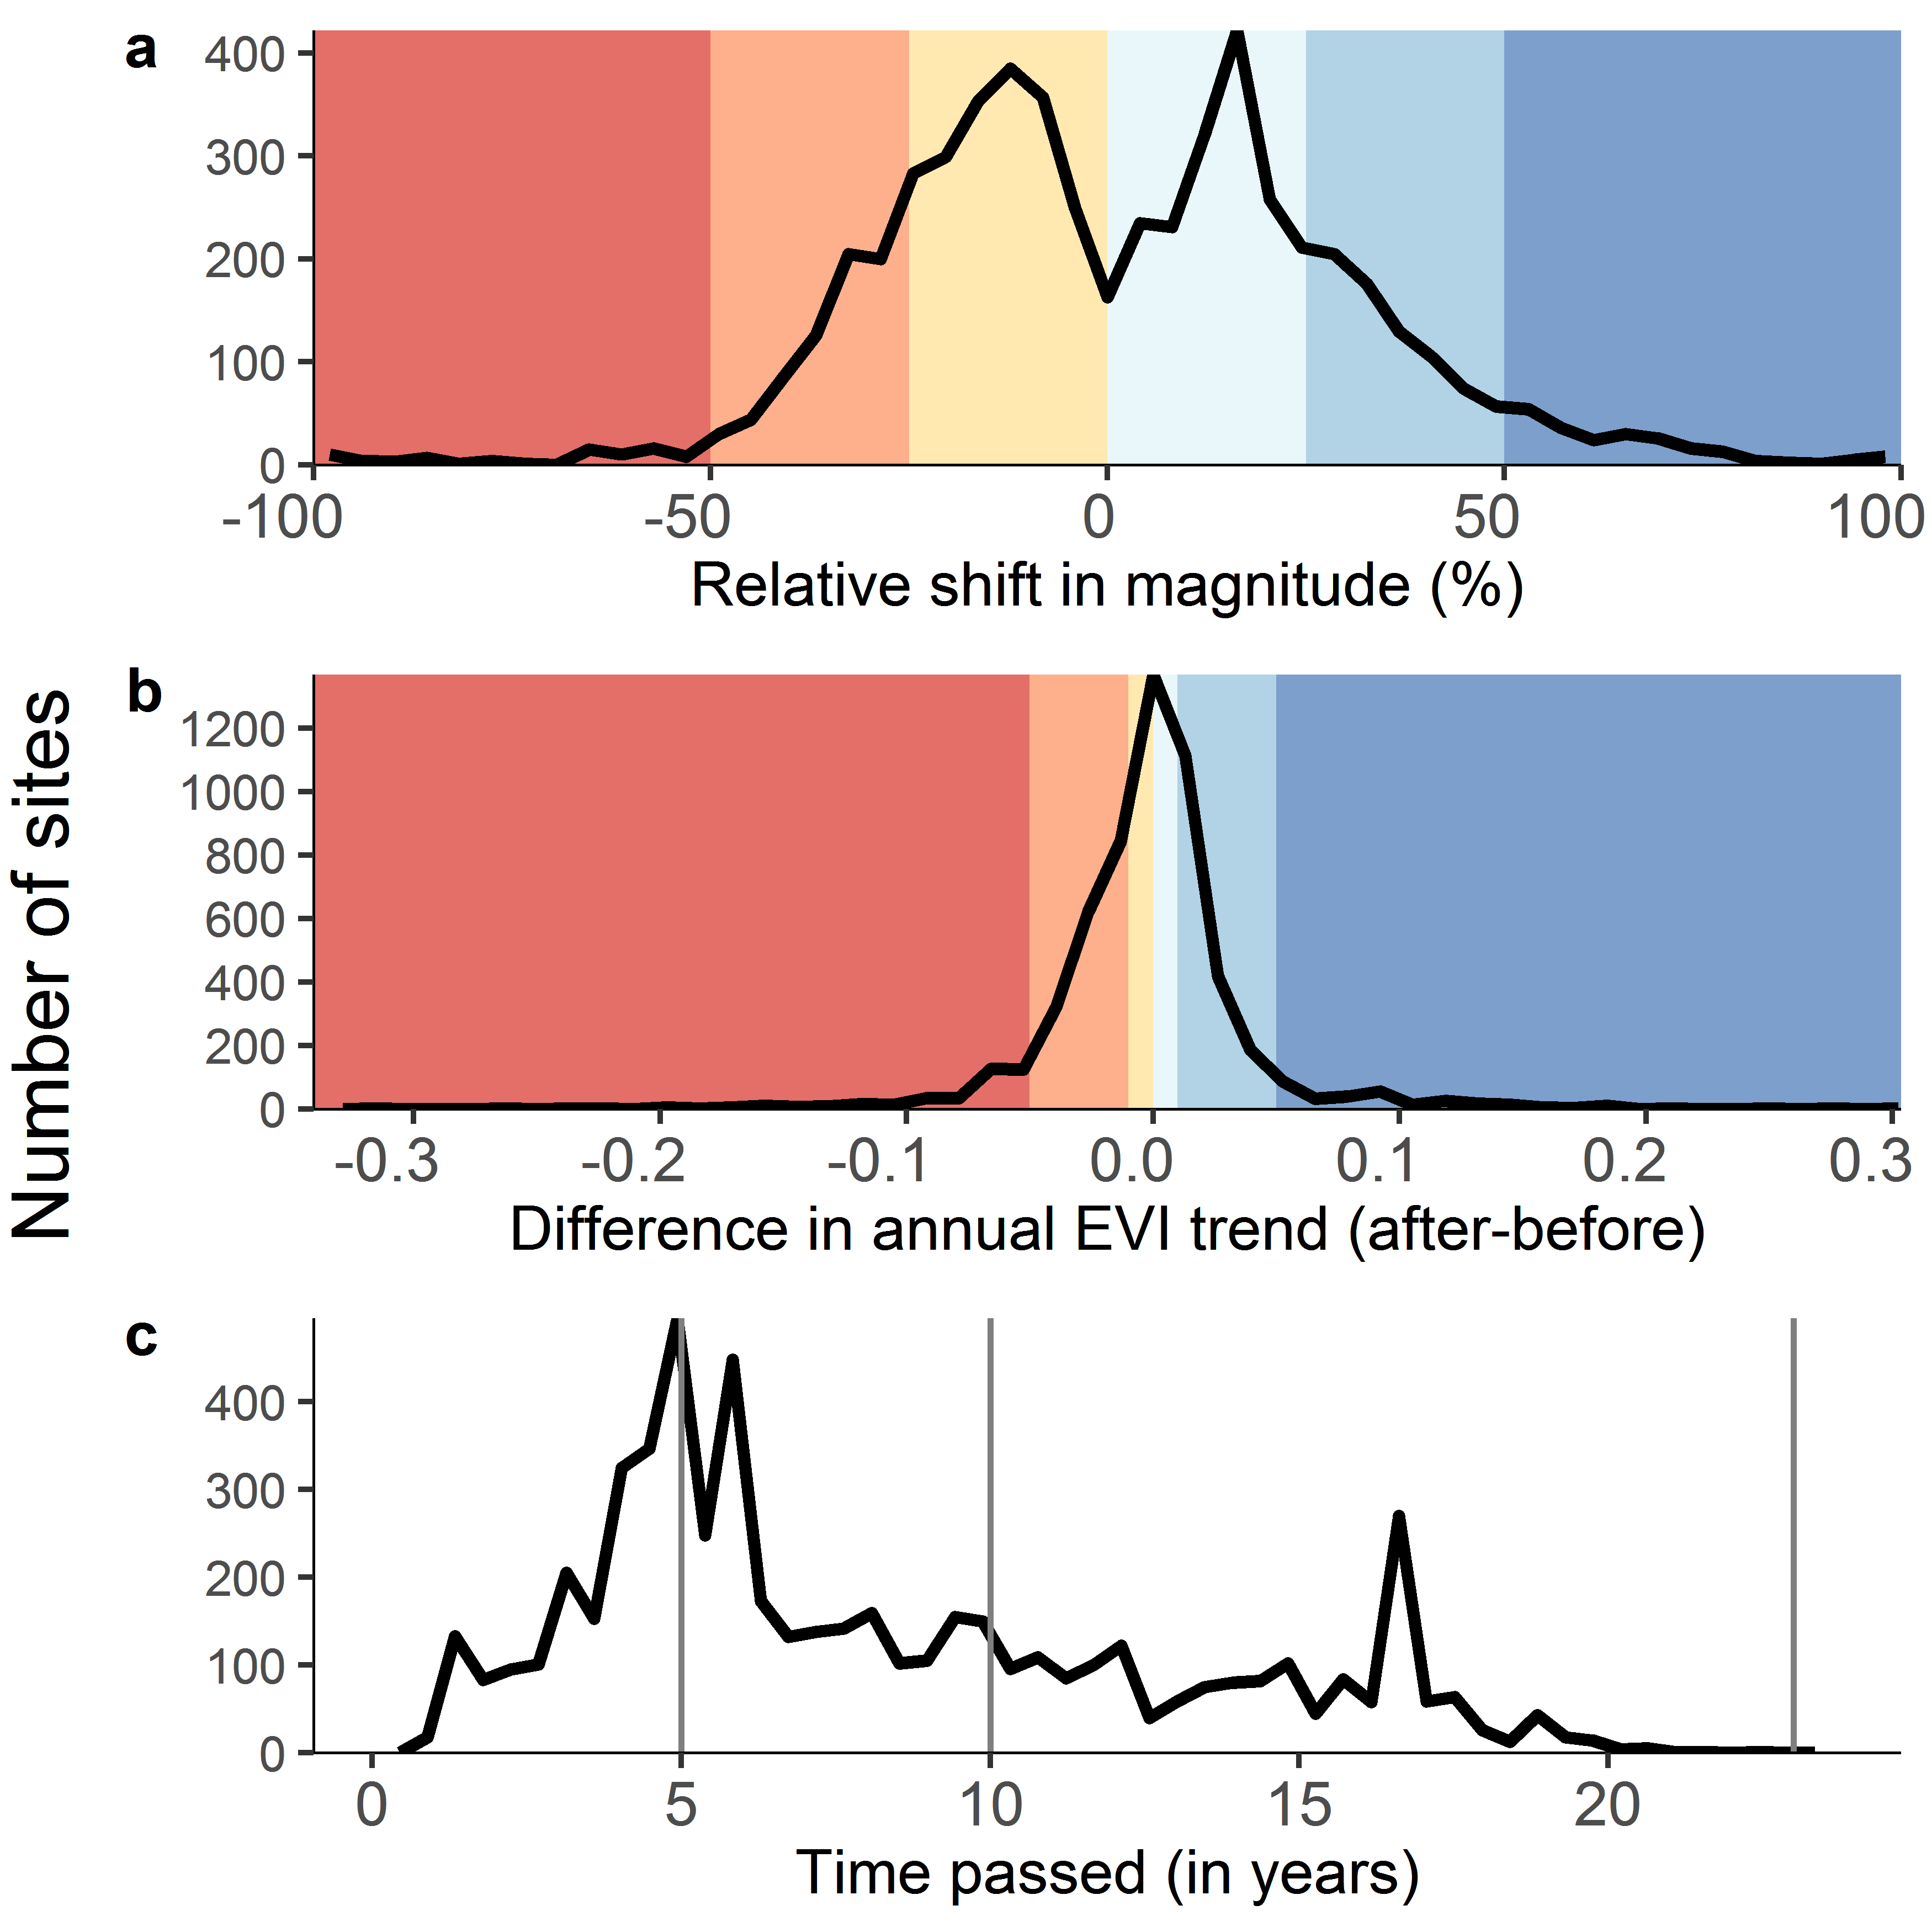
\includegraphics[width=1\textwidth]{chapter3/SI02}
\caption{ Number of sites with abrupt land change per attribute. Number of sites (black line) per attribute of abrupt land change with (\textbf{a}) the relative shift in magnitude, (\textbf{b}) the shift in trend as difference in annual EVI trend, and (\textbf{c}) the time passed between abrupt land change and biodiversity sampling. Background colours in (\textbf{a}) and (\textbf{b}) indicate the binning into six groups for shifts in magnitude (> 50\%, > 25\% to $\leq$ 50\%, and $\leq$ 25\% EVI loss [$---$ to $-$] or gain [$+++$ to $+$]), and in trend (0.01, 0.05, and > 0.05 annual negative [$---$ to $-$] to positive [$+++$ to $+$] EVI trend differences). Gray lines in (\textbf{c}) delineate bins of time passed ($\leq$ 5 years, > 5 and $\leq$ 10 years, and >10 years). Colours as in Figure \ref{F03_02}.}
\label{SI03_02}
\end{figure}

% SI Table 1------ %
% From here https://www.tablesgenerator.com/
\begin{table}[]
\centering
\caption{Number of PREDICTS sites and studies with an abrupt land change. Shown as either a change in magnitude (columns) and/or change in trend (trend). Symbols as in Figure \ref{F03_02}. }
\label{SIT03_01}
\begin{tabular}{@{}lllllllllll@{}}
                                          &                                           & \multicolumn{7}{c}{\textbf{Shift in magnitude}}                                                                                                                                                                    &                               &                             \\
                                          &                                           & \textbf{- - -}             & \textbf{- -}                & \textbf{-}                   & \textbf{0}                    & \textbf{+}                   & \textbf{+ +}                & \textbf{+ + +}              & \textbf{Total sites}          & \textbf{Studies}            \\ \cmidrule(l){3-11} 
                                          & \multicolumn{1}{l|}{- - -}                & 2                          & 8                           & 192                          & NA                            & 73                           & 26                          & 22                          & \cellcolor[HTML]{EFEFEF}323   & \cellcolor[HTML]{C0C0C0}57  \\
                                          & \multicolumn{1}{l|}{- -}                  & 7                          & 281                         & 642                          & NA                            & 497                          & 158                         & 53                          & \cellcolor[HTML]{EFEFEF}1638  & \cellcolor[HTML]{C0C0C0}175 \\
                                          & \multicolumn{1}{l|}{-}                    & 7                          & 88                          & 256                          & NA                            & 231                          & 154                         & 53                          & \cellcolor[HTML]{EFEFEF}789   & \cellcolor[HTML]{C0C0C0}184 \\
                                          & \multicolumn{1}{l|}{0}                    & NA                         & NA                          & NA                           & 10102                         & NA                           & NA                          & NA                          & \cellcolor[HTML]{EFEFEF}10102 & \cellcolor[HTML]{C0C0C0}358 \\
                                          & \multicolumn{1}{l|}{+}                    & 9                          & 102                         & 399                          & NA                            & 410                          & 205                         & 49                          & \cellcolor[HTML]{EFEFEF}1174  & \cellcolor[HTML]{C0C0C0}237 \\
                                          & \multicolumn{1}{l|}{\textbf{+ +}}         & 47                         & 172                         & 342                          & NA                            & 465                          & 254                         & 86                          & \cellcolor[HTML]{EFEFEF}1366  & \cellcolor[HTML]{C0C0C0}224 \\
\multirow{-7}{*}{\textbf{\rotatebox{90}{Shift in trend}}} & \multicolumn{1}{l|}{\textbf{+ + +}}       & 12                         & 137                         & 47                           & NA                            & 34                           & 12                          & 31                          & \cellcolor[HTML]{EFEFEF}273   & \cellcolor[HTML]{C0C0C0}56  \\
                                          & \multicolumn{1}{l|}{\textbf{Total sites}} & \cellcolor[HTML]{EFEFEF}84 & \cellcolor[HTML]{EFEFEF}788 & \cellcolor[HTML]{EFEFEF}1878 & \cellcolor[HTML]{EFEFEF}10102 & \cellcolor[HTML]{EFEFEF}1710 & \cellcolor[HTML]{EFEFEF}809 & \cellcolor[HTML]{EFEFEF}294 &                               &                             \\
                                          & \multicolumn{1}{c|}{\textbf{Studies}}     & \cellcolor[HTML]{C0C0C0}34 & \cellcolor[HTML]{C0C0C0}135 & \cellcolor[HTML]{C0C0C0}246  & \cellcolor[HTML]{C0C0C0}358   & \cellcolor[HTML]{C0C0C0}263  & \cellcolor[HTML]{C0C0C0}171 & \cellcolor[HTML]{C0C0C0}83  &                               &                            
\end{tabular}
\end{table}
% ------ %

% SI - Figure 3 Cross-correlations
\begin{figure}[h]
\centering
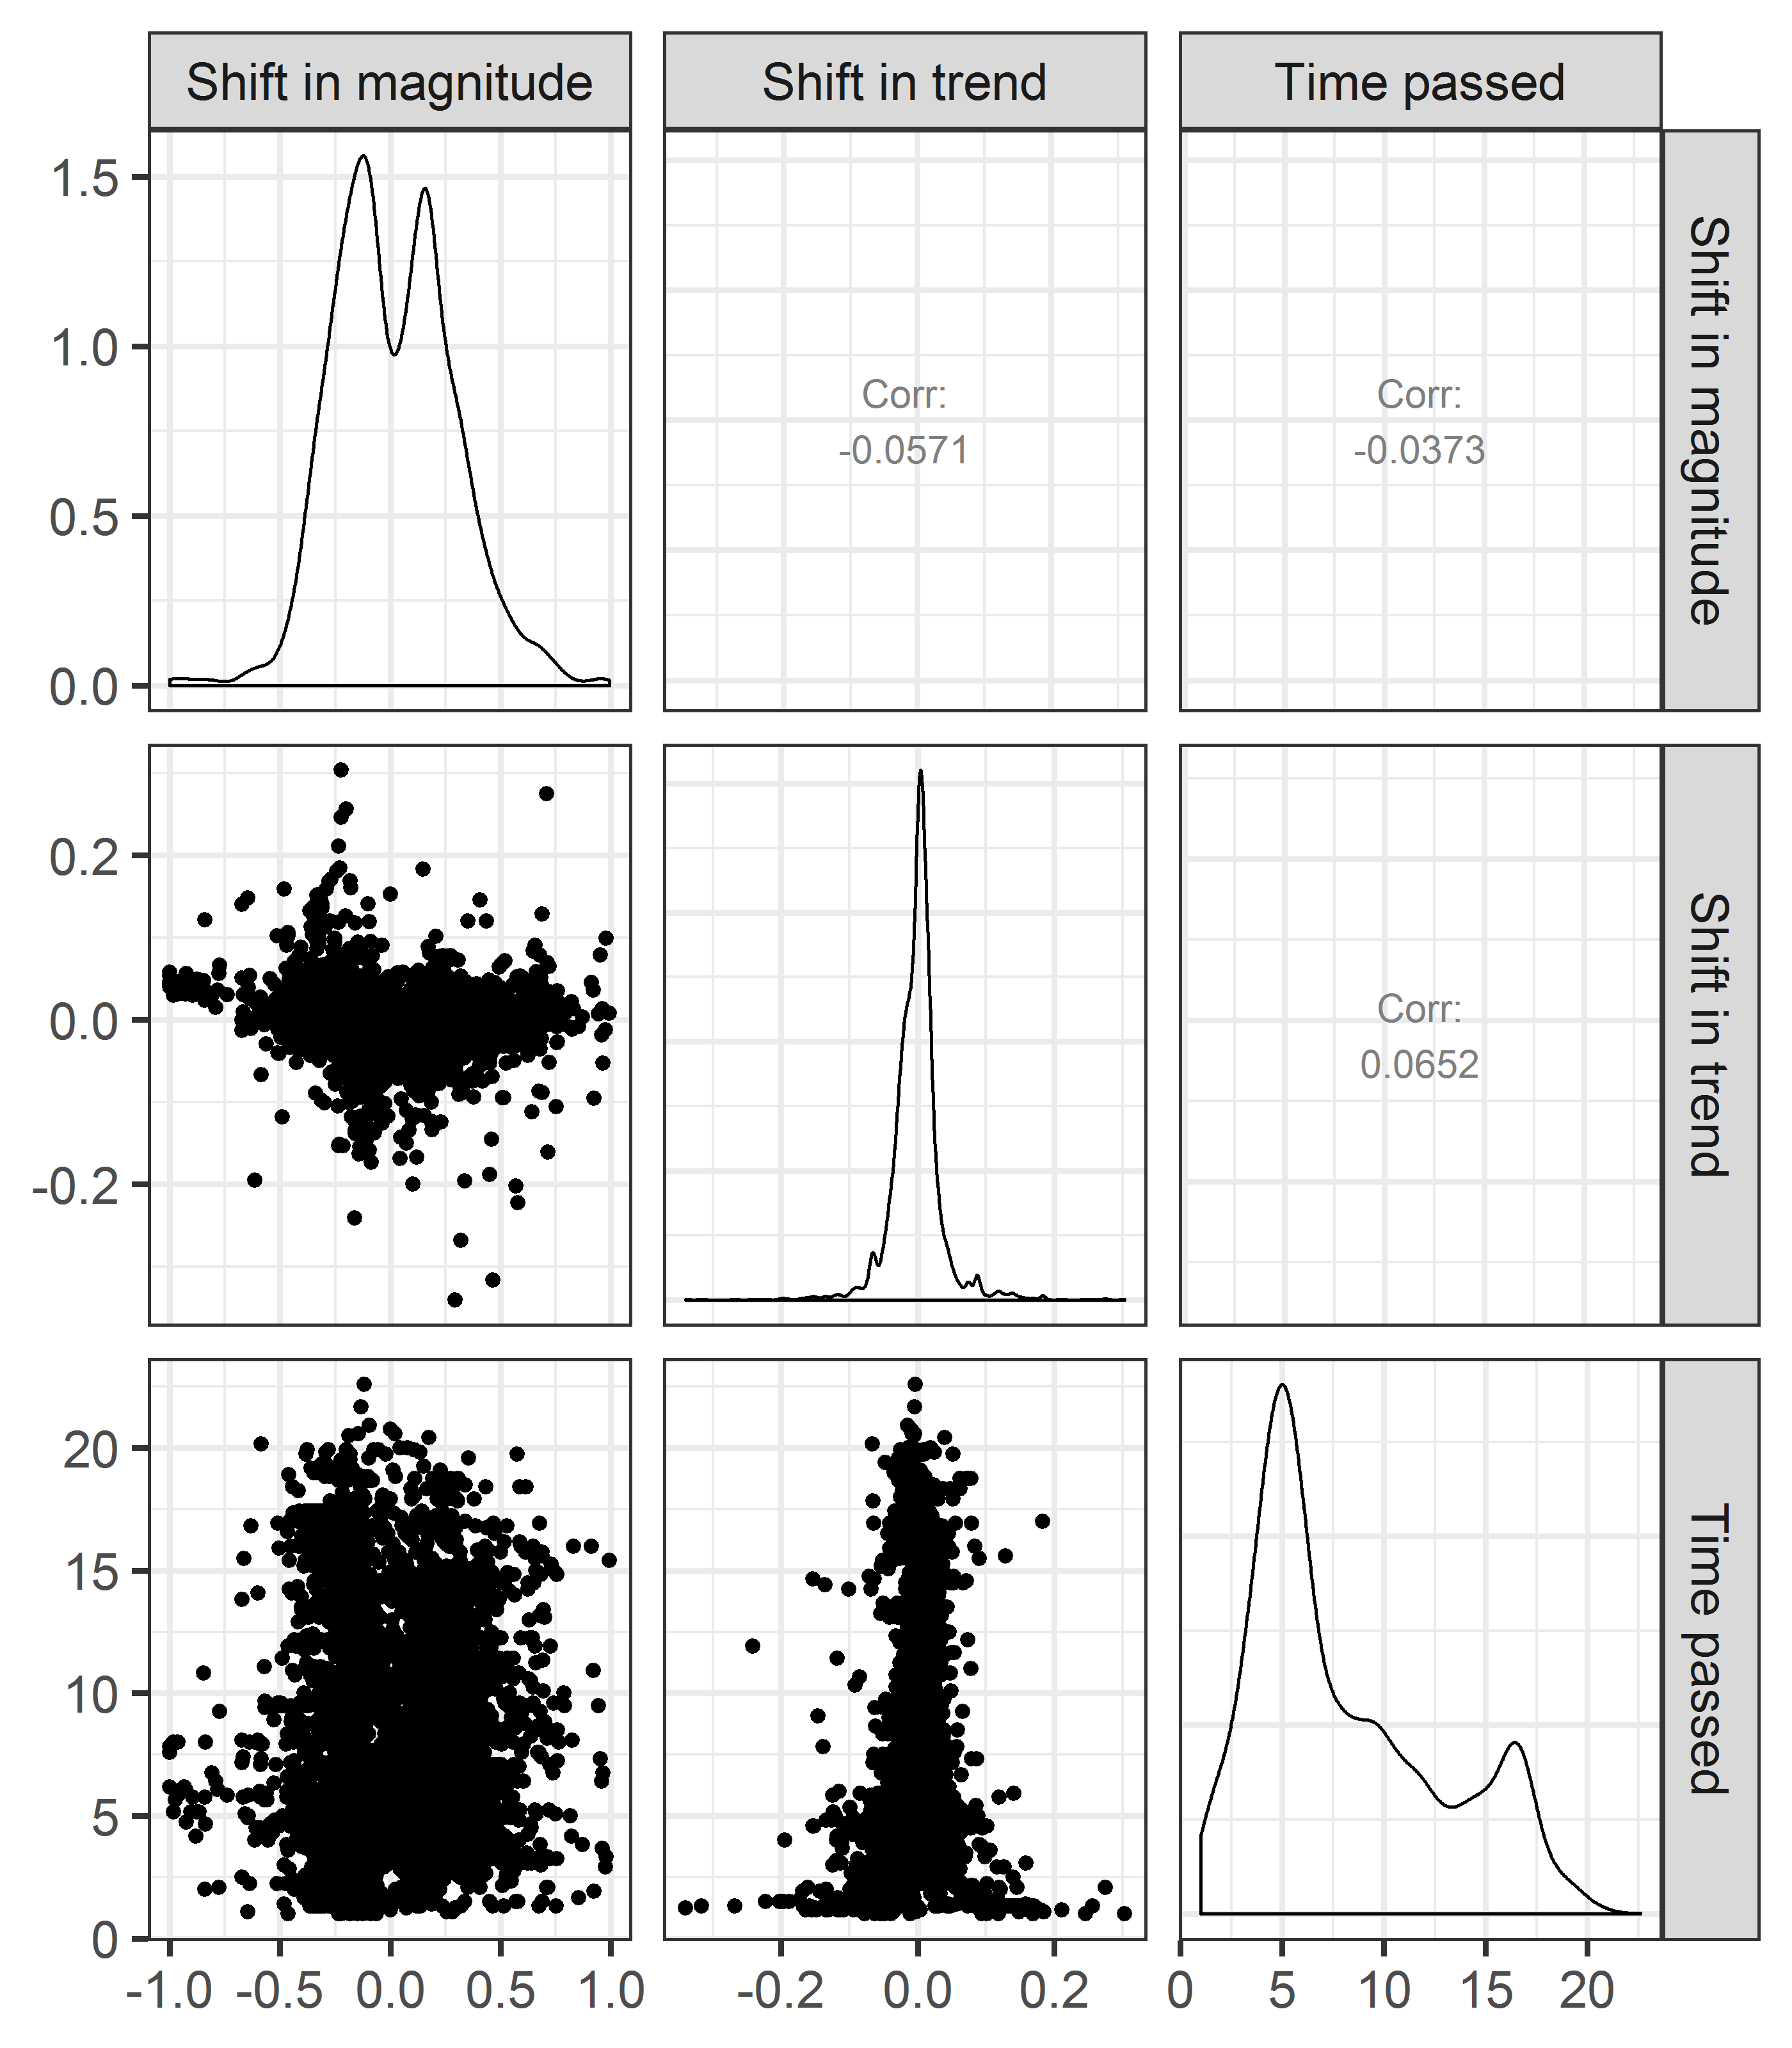
\includegraphics[width=1\textwidth]{chapter3/SI03}
\caption{ Correlations between attributes of abrupt land change. Showing shifts in magnitude, trend and time passed (see Methods). The lower facets show a point density plot, the upper facets the Pearson correlation coefficient between pairs of attributes and the diagonal a density plot.}
\label{SI03_03}
\end{figure}

\endgroup

%---------------------------------------------------
% END DOCUMENT
%---------------------------------------------------
\end{document}
